\documentclass[electronic, oldfontcommands]{kthesis}

%%%%%%%%%%%%%%%%%
%%%% PACKAGES %%%
%%%%%%%%%%%%%%%%%
\usepackage[utf8x]{inputenc}
\usepackage[swedish,english]{babel}
\usepackage{enumerate}  % for capital latin numbers in the list of papers
\usepackage[font=footnotesize]{caption}   % to align the table caption to the right/left
\usepackage{lscape}
%\usepackage{hyperref}  %for references
\usepackage{amsmath,mathrsfs}
\usepackage{amssymb}  % assumes amsmath package installed
\usepackage{epstopdf}
%\usepackage{subfig} % Error I got: Package subcaption Error: This package can't be used in cooperation(subcaption) with the subfig package. \subcaption@CheckCompatibility
\usepackage{cite}
\usepackage{graphicx}
\usepackage{bm}	%Command \bm{make bold}
\usepackage{algorithm}
\usepackage{algpseudocode}
%\usepackage{algpascal} % didn't work with algorithmic environment
\usepackage{multicol}
\usepackage[dvipsnames,table]{xcolor}
\usepackage{lipsum}
%\usepackage[dvipsnames]{xcolor}
% my packages

% Packages added by me
\usepackage{comment}
\usepackage{afterpage} % for changing page color before included papers

%

% Comments
\newcommand{\mk}[1]{{\color{purple} #1}}
\newcommand{\MK}[1]{\textbf{\color{purple} MK: #1}} 

% Text shorts
\newcommand{\etal}{et al.}
\newcommand{\ie}{i.e.}
\newcommand{\eg}{e.g.}
%\newcommand{\etal}{\textit{et al}.}
%\newcommand{\ie}{\textit{i}.\textit{e}.}
%\newcommand{\eg}{\textit{e}.\textit{g}.}

% Dataset names
\def\train{{\text{train}}}
\def\val{{\text{val}}}
\def\test{{\text{test}}}

% Evaluation metrics
\def\ACC{{\text{ACC}}}
\def\BWT{{\text{BWT}}}
\usepackage{subcaption}
%\usepackage{multirow}
\usepackage[shortlabels]{enumitem}
\usepackage{multirow}
\usepackage{wrapfig}

%%% From Taras
%\usepackage[resetlabels, labeled]{multibib}
\usepackage[resetlabels]{multibib}
\usepackage{hyperref}  %for references
\newcites{A}{References}
\newcites{B}{References}
\newcites{C}{References}
\newcites{D}{References}

% https://tex.stackexchange.com/questions/2441/how-to-add-a-forced-line-break-inside-a-table-cell
\usepackage{array}
\usepackage{makecell}

\renewcommand\theadalign{bc}
\renewcommand\theadfont{\bfseries}
\renewcommand\theadgape{\Gape[4pt]}
\renewcommand\cellgape{\Gape[4pt]}

\hypersetup{
	colorlinks = true,
	citecolor = {blue},
	linkcolor=red,
	%menubordercolor = {blue},
	%linkbordercolor = {blue},
}

\def\UrlBreaks{\do\/\do-} % for making proper linebreak in long URL
%\usepackage{breakurl}

\usepackage{tikz}
\usetikzlibrary{tikzmark,calc,decorations.pathreplacing}
\newcommand{\Depth}{2}
\newcommand{\Height}{2}
\newcommand{\Width}{2}

\usetikzlibrary{shapes, arrows}
\usetikzlibrary{calc}
\usetikzlibrary{backgrounds,fit}
\usetikzlibrary{matrix}
\usetikzlibrary{arrows.meta}

% for CNN
\usepackage{amsmath, amssymb, latexsym}
\usepackage[left=2cm,right=2cm,top=2cm,bottom=2cm]{geometry}

\usepackage{pgfplots}
\usetikzlibrary{matrix, positioning, patterns}
\usepgfplotslibrary{groupplots}
\pgfplotsset{compat=newest}

\newlength{\figheight}
\newlength{\figwidth}

\usetikzlibrary{bayesnet}


% Comments
\newcommand{\mk}[1]{{\color{purple} #1}}
\newcommand{\MK}[1]{\textbf{\color{purple} MK: #1}} 

% Text shorts
\newcommand{\etal}{et al.}
\newcommand{\ie}{i.e.}
\newcommand{\eg}{e.g.}
%\newcommand{\etal}{\textit{et al}.}
%\newcommand{\ie}{\textit{i}.\textit{e}.}
%\newcommand{\eg}{\textit{e}.\textit{g}.}

% Dataset names
%\def\train{{\text{train}}}
%\def\val{{\text{val}}}
%\def\test{{\text{test}}}

% Evaluation metrics
\def\ACC{{\text{ACC}}}
\def\BWT{{\text{BWT}}}
\newcommand{\DQN}{\text{DQN}}
\newcommand{\Random}{\text{Random}}
\newcommand{\ETS}{\text{ETS}}
\newcommand{\Heur}{\text{Heur}}
%%%%% NEW MATH DEFINITIONS %%%%%

\usepackage{amsmath,amsfonts,bm}

% Mark sections of captions for referring to divisions of figures
\newcommand{\figleft}{{\em (Left)}}
\newcommand{\figcenter}{{\em (Center)}}
\newcommand{\figright}{{\em (Right)}}
\newcommand{\figtop}{{\em (Top)}}
\newcommand{\figbottom}{{\em (Bottom)}}
\newcommand{\captiona}{{\em (a)}}
\newcommand{\captionb}{{\em (b)}}
\newcommand{\captionc}{{\em (c)}}
\newcommand{\captiond}{{\em (d)}}

% Highlight a newly defined term
\newcommand{\newterm}[1]{{\bf #1}}


% Figure reference, lower-case.
\def\figref#1{figure~\ref{#1}}
% Figure reference, capital. For start of sentence
\def\Figref#1{Figure~\ref{#1}}
\def\twofigref#1#2{figures \ref{#1} and \ref{#2}}
\def\quadfigref#1#2#3#4{figures \ref{#1}, \ref{#2}, \ref{#3} and \ref{#4}}
% Section reference, lower-case.
\def\secref#1{section~\ref{#1}}
% Section reference, capital.
\def\Secref#1{Section~\ref{#1}}
% Reference to two sections.
\def\twosecrefs#1#2{sections \ref{#1} and \ref{#2}}
% Reference to three sections.
\def\secrefs#1#2#3{sections \ref{#1}, \ref{#2} and \ref{#3}}
% Reference to an equation, lower-case.
\def\eqref#1{equation~\ref{#1}}
% Reference to an equation, upper case
\def\Eqref#1{Equation~\ref{#1}}
% A raw reference to an equation---avoid using if possible
\def\plaineqref#1{\ref{#1}}
% Reference to a chapter, lower-case.
\def\chapref#1{chapter~\ref{#1}}
% Reference to an equation, upper case.
\def\Chapref#1{Chapter~\ref{#1}}
% Reference to a range of chapters
\def\rangechapref#1#2{chapters\ref{#1}--\ref{#2}}
% Reference to an algorithm, lower-case.
\def\algref#1{algorithm~\ref{#1}}
% Reference to an algorithm, upper case.
\def\Algref#1{Algorithm~\ref{#1}}
\def\twoalgref#1#2{algorithms \ref{#1} and \ref{#2}}
\def\Twoalgref#1#2{Algorithms \ref{#1} and \ref{#2}}
% Reference to a part, lower case
\def\partref#1{part~\ref{#1}}
% Reference to a part, upper case
\def\Partref#1{Part~\ref{#1}}
\def\twopartref#1#2{parts \ref{#1} and \ref{#2}}

\def\ceil#1{\lceil #1 \rceil}
\def\floor#1{\lfloor #1 \rfloor}
\def\1{\bm{1}}
\newcommand{\train}{\mathcal{D}}
\newcommand{\valid}{\mathcal{D_{\mathrm{valid}}}}
\newcommand{\test}{\mathcal{D_{\mathrm{test}}}}

\def\eps{{\epsilon}}


% Random variables
\def\reta{{\textnormal{$\eta$}}}
\def\ra{{\textnormal{a}}}
\def\rb{{\textnormal{b}}}
\def\rc{{\textnormal{c}}}
\def\rd{{\textnormal{d}}}
\def\re{{\textnormal{e}}}
\def\rf{{\textnormal{f}}}
\def\rg{{\textnormal{g}}}
\def\rh{{\textnormal{h}}}
\def\ri{{\textnormal{i}}}
\def\rj{{\textnormal{j}}}
\def\rk{{\textnormal{k}}}
\def\rl{{\textnormal{l}}}
% rm is already a command, just don't name any random variables m
\def\rn{{\textnormal{n}}}
\def\ro{{\textnormal{o}}}
\def\rp{{\textnormal{p}}}
\def\rq{{\textnormal{q}}}
\def\rr{{\textnormal{r}}}
\def\rs{{\textnormal{s}}}
\def\rt{{\textnormal{t}}}
\def\ru{{\textnormal{u}}}
\def\rv{{\textnormal{v}}}
\def\rw{{\textnormal{w}}}
\def\rx{{\textnormal{x}}}
\def\ry{{\textnormal{y}}}
\def\rz{{\textnormal{z}}}

% Random vectors
\def\rvepsilon{{\mathbf{\epsilon}}}
\def\rvtheta{{\mathbf{\theta}}}
\def\rva{{\mathbf{a}}}
\def\rvb{{\mathbf{b}}}
\def\rvc{{\mathbf{c}}}
\def\rvd{{\mathbf{d}}}
\def\rve{{\mathbf{e}}}
\def\rvf{{\mathbf{f}}}
\def\rvg{{\mathbf{g}}}
\def\rvh{{\mathbf{h}}}
\def\rvu{{\mathbf{i}}}
\def\rvj{{\mathbf{j}}}
\def\rvk{{\mathbf{k}}}
\def\rvl{{\mathbf{l}}}
\def\rvm{{\mathbf{m}}}
\def\rvn{{\mathbf{n}}}
\def\rvo{{\mathbf{o}}}
\def\rvp{{\mathbf{p}}}
\def\rvq{{\mathbf{q}}}
\def\rvr{{\mathbf{r}}}
\def\rvs{{\mathbf{s}}}
\def\rvt{{\mathbf{t}}}
\def\rvu{{\mathbf{u}}}
\def\rvv{{\mathbf{v}}}
\def\rvw{{\mathbf{w}}}
\def\rvx{{\mathbf{x}}}
\def\rvy{{\mathbf{y}}}
\def\rvz{{\mathbf{z}}}

% Elements of random vectors
\def\erva{{\textnormal{a}}}
\def\ervb{{\textnormal{b}}}
\def\ervc{{\textnormal{c}}}
\def\ervd{{\textnormal{d}}}
\def\erve{{\textnormal{e}}}
\def\ervf{{\textnormal{f}}}
\def\ervg{{\textnormal{g}}}
\def\ervh{{\textnormal{h}}}
\def\ervi{{\textnormal{i}}}
\def\ervj{{\textnormal{j}}}
\def\ervk{{\textnormal{k}}}
\def\ervl{{\textnormal{l}}}
\def\ervm{{\textnormal{m}}}
\def\ervn{{\textnormal{n}}}
\def\ervo{{\textnormal{o}}}
\def\ervp{{\textnormal{p}}}
\def\ervq{{\textnormal{q}}}
\def\ervr{{\textnormal{r}}}
\def\ervs{{\textnormal{s}}}
\def\ervt{{\textnormal{t}}}
\def\ervu{{\textnormal{u}}}
\def\ervv{{\textnormal{v}}}
\def\ervw{{\textnormal{w}}}
\def\ervx{{\textnormal{x}}}
\def\ervy{{\textnormal{y}}}
\def\ervz{{\textnormal{z}}}

% Random matrices
\def\rmA{{\mathbf{A}}}
\def\rmB{{\mathbf{B}}}
\def\rmC{{\mathbf{C}}}
\def\rmD{{\mathbf{D}}}
\def\rmE{{\mathbf{E}}}
\def\rmF{{\mathbf{F}}}
\def\rmG{{\mathbf{G}}}
\def\rmH{{\mathbf{H}}}
\def\rmI{{\mathbf{I}}}
\def\rmJ{{\mathbf{J}}}
\def\rmK{{\mathbf{K}}}
\def\rmL{{\mathbf{L}}}
\def\rmM{{\mathbf{M}}}
\def\rmN{{\mathbf{N}}}
\def\rmO{{\mathbf{O}}}
\def\rmP{{\mathbf{P}}}
\def\rmQ{{\mathbf{Q}}}
\def\rmR{{\mathbf{R}}}
\def\rmS{{\mathbf{S}}}
\def\rmT{{\mathbf{T}}}
\def\rmU{{\mathbf{U}}}
\def\rmV{{\mathbf{V}}}
\def\rmW{{\mathbf{W}}}
\def\rmX{{\mathbf{X}}}
\def\rmY{{\mathbf{Y}}}
\def\rmZ{{\mathbf{Z}}}

% Elements of random matrices
\def\ermA{{\textnormal{A}}}
\def\ermB{{\textnormal{B}}}
\def\ermC{{\textnormal{C}}}
\def\ermD{{\textnormal{D}}}
\def\ermE{{\textnormal{E}}}
\def\ermF{{\textnormal{F}}}
\def\ermG{{\textnormal{G}}}
\def\ermH{{\textnormal{H}}}
\def\ermI{{\textnormal{I}}}
\def\ermJ{{\textnormal{J}}}
\def\ermK{{\textnormal{K}}}
\def\ermL{{\textnormal{L}}}
\def\ermM{{\textnormal{M}}}
\def\ermN{{\textnormal{N}}}
\def\ermO{{\textnormal{O}}}
\def\ermP{{\textnormal{P}}}
\def\ermQ{{\textnormal{Q}}}
\def\ermR{{\textnormal{R}}}
\def\ermS{{\textnormal{S}}}
\def\ermT{{\textnormal{T}}}
\def\ermU{{\textnormal{U}}}
\def\ermV{{\textnormal{V}}}
\def\ermW{{\textnormal{W}}}
\def\ermX{{\textnormal{X}}}
\def\ermY{{\textnormal{Y}}}
\def\ermZ{{\textnormal{Z}}}

% Vectors
\def\vzero{{\bm{0}}}
\def\vone{{\bm{1}}}
\def\vmu{{\bm{\mu}}}
\def\vsigma{{\bm{\sigma}}}
\def\vepsilon{{\bm{\epsilon}}}
\def\vtheta{{\bm{\theta}}}
\def\vphi{{\bm{\phi}}}
\def\vpi{{\bm{\pi}}}
\def\vlambda{{\bm{\lambda}}}
\def\vvarphi{{\bm{\varphi}}}
\def\vI{{\bm{I}}} % for representing image
\def\va{{\bm{a}}}
\def\vb{{\bm{b}}}
\def\vc{{\bm{c}}}
\def\vd{{\bm{d}}}
\def\ve{{\bm{e}}}
\def\vf{{\bm{f}}}
\def\vg{{\bm{g}}}
\def\vh{{\bm{h}}}
\def\vi{{\bm{i}}}
\def\vj{{\bm{j}}}
\def\vk{{\bm{k}}}
\def\vl{{\bm{l}}}
\def\vm{{\bm{m}}}
\def\vn{{\bm{n}}}
\def\vo{{\bm{o}}}
\def\vp{{\bm{p}}}
\def\vq{{\bm{q}}}
\def\vr{{\bm{r}}}
\def\vs{{\bm{s}}}
\def\vt{{\bm{t}}}
\def\vu{{\bm{u}}}
\def\vv{{\bm{v}}}
\def\vw{{\bm{w}}}
\def\vx{{\bm{x}}}
\def\vy{{\bm{y}}}
\def\vz{{\bm{z}}}

% Elements of vectors
\def\evalpha{{\alpha}}
\def\evbeta{{\beta}}
\def\evepsilon{{\epsilon}}
\def\evlambda{{\lambda}}
\def\evomega{{\omega}}
\def\evmu{{\mu}}
\def\evpsi{{\psi}}
\def\evsigma{{\sigma}}
\def\evtheta{{\theta}}
\def\eva{{a}}
\def\evb{{b}}
\def\evc{{c}}
\def\evd{{d}}
\def\eve{{e}}
\def\evf{{f}}
\def\evg{{g}}
\def\evh{{h}}
\def\evi{{i}}
\def\evj{{j}}
\def\evk{{k}}
\def\evl{{l}}
\def\evm{{m}}
\def\evn{{n}}
\def\evo{{o}}
\def\evp{{p}}
\def\evq{{q}}
\def\evr{{r}}
\def\evs{{s}}
\def\evt{{t}}
\def\evu{{u}}
\def\evv{{v}}
\def\evw{{w}}
\def\evx{{x}}
\def\evy{{y}}
\def\evz{{z}}

% Matrix
\def\mA{{\bm{A}}}
\def\mB{{\bm{B}}}
\def\mC{{\bm{C}}}
\def\mD{{\bm{D}}}
\def\mE{{\bm{E}}}
\def\mF{{\bm{F}}}
\def\mG{{\bm{G}}}
\def\mH{{\bm{H}}}
\def\mI{{\bm{I}}}
\def\mJ{{\bm{J}}}
\def\mK{{\bm{K}}}
\def\mL{{\bm{L}}}
\def\mM{{\bm{M}}}
\def\mN{{\bm{N}}}
\def\mO{{\bm{O}}}
\def\mP{{\bm{P}}}
\def\mQ{{\bm{Q}}}
\def\mR{{\bm{R}}}
\def\mS{{\bm{S}}}
\def\mT{{\bm{T}}}
\def\mU{{\bm{U}}}
\def\mV{{\bm{V}}}
\def\mW{{\bm{W}}}
\def\mX{{\bm{X}}}
\def\mY{{\bm{Y}}}
\def\mZ{{\bm{Z}}}
\def\mBeta{{\bm{\beta}}}
\def\mPhi{{\bm{\Phi}}}
\def\mLambda{{\bm{\Lambda}}}
\def\mSigma{{\bm{\Sigma}}}

% Tensor
\DeclareMathAlphabet{\mathsfit}{\encodingdefault}{\sfdefault}{m}{sl}
\SetMathAlphabet{\mathsfit}{bold}{\encodingdefault}{\sfdefault}{bx}{n}
\newcommand{\tens}[1]{\bm{\mathsfit{#1}}}
\def\tA{{\tens{A}}}
\def\tB{{\tens{B}}}
\def\tC{{\tens{C}}}
\def\tD{{\tens{D}}}
\def\tE{{\tens{E}}}
\def\tF{{\tens{F}}}
\def\tG{{\tens{G}}}
\def\tH{{\tens{H}}}
\def\tI{{\tens{I}}}
\def\tJ{{\tens{J}}}
\def\tK{{\tens{K}}}
\def\tL{{\tens{L}}}
\def\tM{{\tens{M}}}
\def\tN{{\tens{N}}}
\def\tO{{\tens{O}}}
\def\tP{{\tens{P}}}
\def\tQ{{\tens{Q}}}
\def\tR{{\tens{R}}}
\def\tS{{\tens{S}}}
\def\tT{{\tens{T}}}
\def\tU{{\tens{U}}}
\def\tV{{\tens{V}}}
\def\tW{{\tens{W}}}
\def\tX{{\tens{X}}}
\def\tY{{\tens{Y}}}
\def\tZ{{\tens{Z}}}


% Graph
\def\gA{{\mathcal{A}}}
\def\gB{{\mathcal{B}}}
\def\gC{{\mathcal{C}}}
\def\gD{{\mathcal{D}}}
\def\gE{{\mathcal{E}}}
\def\gF{{\mathcal{F}}}
\def\gG{{\mathcal{G}}}
\def\gH{{\mathcal{H}}}
\def\gI{{\mathcal{I}}}
\def\gJ{{\mathcal{J}}}
\def\gK{{\mathcal{K}}}
\def\gL{{\mathcal{L}}}
\def\gM{{\mathcal{M}}}
\def\gN{{\mathcal{N}}}
\def\gO{{\mathcal{O}}}
\def\gP{{\mathcal{P}}}
\def\gQ{{\mathcal{Q}}}
\def\gR{{\mathcal{R}}}
\def\gS{{\mathcal{S}}}
\def\gT{{\mathcal{T}}}
\def\gU{{\mathcal{U}}}
\def\gV{{\mathcal{V}}}
\def\gW{{\mathcal{W}}}
\def\gX{{\mathcal{X}}}
\def\gY{{\mathcal{Y}}}
\def\gZ{{\mathcal{Z}}}

% Sets
\def\sA{{\mathbb{A}}}
\def\sB{{\mathbb{B}}}
\def\sC{{\mathbb{C}}}
\def\sD{{\mathbb{D}}}
% Don't use a set called E, because this would be the same as our symbol
% for expectation.
\def\sF{{\mathbb{F}}}
\def\sG{{\mathbb{G}}}
\def\sH{{\mathbb{H}}}
\def\sI{{\mathbb{I}}}
\def\sJ{{\mathbb{J}}}
\def\sK{{\mathbb{K}}}
\def\sL{{\mathbb{L}}}
\def\sM{{\mathbb{M}}}
\def\sN{{\mathbb{N}}}
\def\sO{{\mathbb{O}}}
\def\sP{{\mathbb{P}}}
\def\sQ{{\mathbb{Q}}}
\def\sR{{\mathbb{R}}}
\def\sS{{\mathbb{S}}}
\def\sT{{\mathbb{T}}}
\def\sU{{\mathbb{U}}}
\def\sV{{\mathbb{V}}}
\def\sW{{\mathbb{W}}}
\def\sX{{\mathbb{X}}}
\def\sY{{\mathbb{Y}}}
\def\sZ{{\mathbb{Z}}}

% Entries of a matrix
\def\emLambda{{\Lambda}}
\def\emA{{A}}
\def\emB{{B}}
\def\emC{{C}}
\def\emD{{D}}
\def\emE{{E}}
\def\emF{{F}}
\def\emG{{G}}
\def\emH{{H}}
\def\emI{{I}}
\def\emJ{{J}}
\def\emK{{K}}
\def\emL{{L}}
\def\emM{{M}}
\def\emN{{N}}
\def\emO{{O}}
\def\emP{{P}}
\def\emQ{{Q}}
\def\emR{{R}}
\def\emS{{S}}
\def\emT{{T}}
\def\emU{{U}}
\def\emV{{V}}
\def\emW{{W}}
\def\emX{{X}}
\def\emY{{Y}}
\def\emZ{{Z}}
\def\emSigma{{\Sigma}}

% entries of a tensor
% Same font as tensor, without \bm wrapper
\newcommand{\etens}[1]{\mathsfit{#1}}
\def\etLambda{{\etens{\Lambda}}}
\def\etA{{\etens{A}}}
\def\etB{{\etens{B}}}
\def\etC{{\etens{C}}}
\def\etD{{\etens{D}}}
\def\etE{{\etens{E}}}
\def\etF{{\etens{F}}}
\def\etG{{\etens{G}}}
\def\etH{{\etens{H}}}
\def\etI{{\etens{I}}}
\def\etJ{{\etens{J}}}
\def\etK{{\etens{K}}}
\def\etL{{\etens{L}}}
\def\etM{{\etens{M}}}
\def\etN{{\etens{N}}}
\def\etO{{\etens{O}}}
\def\etP{{\etens{P}}}
\def\etQ{{\etens{Q}}}
\def\etR{{\etens{R}}}
\def\etS{{\etens{S}}}
\def\etT{{\etens{T}}}
\def\etU{{\etens{U}}}
\def\etV{{\etens{V}}}
\def\etW{{\etens{W}}}
\def\etX{{\etens{X}}}
\def\etY{{\etens{Y}}}
\def\etZ{{\etens{Z}}}

% The true underlying data generating distribution
\newcommand{\pdata}{p_{\rm{data}}}
% The empirical distribution defined by the training set
\newcommand{\ptrain}{\hat{p}_{\rm{data}}}
\newcommand{\Ptrain}{\hat{P}_{\rm{data}}}
% The model distribution
\newcommand{\pmodel}{p_{\rm{model}}}
\newcommand{\Pmodel}{P_{\rm{model}}}
\newcommand{\ptildemodel}{\tilde{p}_{\rm{model}}}
% Stochastic autoencoder distributions
\newcommand{\pencode}{p_{\rm{encoder}}}
\newcommand{\pdecode}{p_{\rm{decoder}}}
\newcommand{\precons}{p_{\rm{reconstruct}}}

\newcommand{\laplace}{\mathrm{Laplace}} % Laplace distribution

\newcommand{\E}{\mathbb{E}}
\newcommand{\Ls}{\mathcal{L}}
\newcommand{\R}{\mathbb{R}}
\newcommand{\emp}{\tilde{p}}
\newcommand{\lr}{\alpha}
\newcommand{\reg}{\lambda}
\newcommand{\rect}{\mathrm{rectifier}}
\newcommand{\softmax}{\mathrm{softmax}}
\newcommand{\sigmoid}{\sigma}
\newcommand{\softplus}{\zeta}
\newcommand{\KL}{D_{\mathrm{KL}}}
\newcommand{\Var}{\mathrm{Var}}
\newcommand{\standarderror}{\mathrm{SE}}
\newcommand{\Cov}{\mathrm{Cov}}
% Wolfram Mathworld says $L^2$ is for function spaces and $\ell^2$ is for vectors
% But then they seem to use $L^2$ for vectors throughout the site, and so does
% wikipedia.
\newcommand{\normlzero}{L^0}
\newcommand{\normlone}{L^1}
\newcommand{\normltwo}{L^2}
\newcommand{\normlp}{L^p}
\newcommand{\normmax}{L^\infty}

\newcommand{\parents}{Pa} % See usage in notation.tex. Chosen to match Daphne's book.

%\DeclareMathOperator*{\max}{max}
\DeclareMathOperator*{\argmax}{arg\,max}
\DeclareMathOperator*{\argmin}{arg\,min}

\DeclareMathOperator{\sign}{sign}
\DeclareMathOperator{\Tr}{Tr}
\let\ab\allowbreak



\makeatletter
%\@addtoreset{section}{part}
%\renewcommand\part{\thispagestyle{empty}}
%%% All this for removing page number on part environment
%%% See https://latex.org/forum/viewtopic.php?t=4293
\renewcommand\part{%
	\if@openright
	\cleardoublepage
	\else
	\clearpage
	\fi
	\thispagestyle{empty}%
	\if@twocolumn
	\onecolumn
	\@tempswatrue
	\else
	\@tempswafalse
	\fi
	\null\vfil
	\secdef\@part\@spart}
%%%
%\newcommand{\insubfile}[1]{\ifx\@onlypreamble\@notprerr\else#1\fi}

%%% Command that fixed correct chapter and section referencing when setting chapter counter to zero in Part 2
%%% Still had to reset counter in Part 2 with \setcounter{chapter}{0}, which they didn't do in https://tex.stackexchange.com/questions/54383/how-to-reset-chapter-and-section-counter-with-part
\@addtoreset{chapter}{part}
\makeatother

%%%%%%%%%%%%%%%%%%%%%%%%%%%%%%%%%%%%%%%
%%%%%%%%% Document starts here %%%%%%%%
%%%%%%%%%%%%%%%%%%%%%%%%%%%%%%%%%%%%%%%
\begin{document}
	
% for reducing the space between text and equation environments
\setlength{\abovedisplayskip}{3pt} 
\setlength{\belowdisplayskip}{3pt}
	
\newcommand*{\BuildingFromMainFile}{}
	
%%%%%%%%%%%%%%%%%%%%%%%%%%%%%%%%%%%%%%%%%%
%%%%%% First and second pages %%%%%%%%%%%%
%%%%%%%%%%%%%%%%%%%%%%%%%%%%%%%%%%%%%%%%%%
\title{Fine-Grained and Continual Visual Recognition for Assisting Visually Impaired People}
%\subtitle{\textbf{sub-title}}
\author{Marcus Klasson}
\date{date}
\thesistype{Doctoral Thesis}
\imprint{Stockholm, Sweden, 2022}
\examen{Teknologie doktorexamen i datalogi}
\disputationsdatum{tisdagen den 8 november 2022 klockan 9.00}
\disputationslokal{Sal F3, Lindstedtsvägen 26, Kungliga Tekniska H\"{o}gskolan, Stockholm}
\publisher{Universitetsservice US AB}
\address{KTH Royal Institute of Technology \\School of Electrical Engineering and Computer Science\\ Division of Robotics, Perception, and Learning \\ SE-10044 Stockholm, Sweden}
\isbn{ISBN 100-}
%\issn{ISSN XXX} % No longer used at KTH
\trita{TRITA-EECS-AVL-2020:4}
\kthlogo{KTHLogo}
	
% Create title page using info above
\maketitle

\frontmatter % Pages i, ii, iii, iv, v etc.
%%%%%%%%%%%%%%%%%%%%%%%%%%%%%%%%%%%
%%%%%%%%%%% ABSTRACT %%%%%%%%%%%%%%
%%%%%%%%%%%%%%%%%%%%%%%%%%%%%%%%%%%
\begin{abstract}

\noindent In recent years, computer vision-based assistive technologies have enabled visually impaired people to use automatic visual recognition on their mobile phones. 
These systems should be capable of recognizing objects on fine-grained levels to provide the user with accurate predictions. Additionally, the user should have the option to update the system continuously to recognize new objects of interest. 
However, there are several challenges that need to be tackled to enable such features with assistive vision systems in real and highly-varying environments. 
For instance, fine-grained image recognition usually requires large amounts of labeled data to be robust. %, and
Moreover, image classifiers struggle with retaining performance of previously learned abilities when they are adapted %adapting 
to new tasks. 
This thesis is divided into two parts where we address these challenges. 
First, we focus on the application of using assistive vision systems for grocery shopping, where items are naturally structured based on fine-grained details.  
We demonstrate how image classifiers can be trained with a combination of natural images and web-scraped information about the groceries to obtain more accurate classification performance compared to only using natural images for training. 
Thereafter, we bring forward a new approach for continual learning called replay scheduling, where we select which tasks to replay at different times to improve memory retention. 
Furthermore, we propose a novel framework for learning replay scheduling policies that can generalize to new continual learning scenarios for mitigating the catastrophic forgetting effect in image classifiers. 
This thesis provides insights on practical challenges that need to be addressed to enhance the usefulness of computer vision for assisting the visually impaired in real-world scenarios. 

\begin{comment}
\noindent In recent years, computer vision-based assistive technologies have enabled visually impaired people to use automatic visual recognition on their mobile phones. 
These systems should be capable of recognizing objects on fine-grained levels to provide the user with accurate predictions. Additionally, the user should have the option to update the system continuously to recognize new objects of interest.  %Moreover, a valuable feature would be if they could be updated to recognize new object classes. 
However, there are several challenges that need to be tackled to enable such features with assistive vision systems in real and highly-varying environments. 
For instance, fine-grained image recognition usually requires large amounts of labeled data to be robust, and image classifiers struggle with retaining performance of previously learned abilities when adapting to new tasks. 
This thesis is divided into two parts where we address these challenges. 
First, we focus on the application of using assistive vision devices for grocery shopping where items are naturally structured based on fine-grained details.  %grocery shopping with an assistive vision device where items are naturally structured based on fine-grained details. 
We demonstrate how image classifiers can be trained with a combination of natural images and web-scraped information about the groceries to obtain more accurate classification performance compared to only using natural images for training. %To reduce the need for exhaustive data collection in grocery stores, we show how image classifiers can be trained with a combination of real images and web-scraped information about the groceries to obtain more accurate classification performance.
Secondly, we bring forward a new approach for continual learning called replay scheduling where we select which tasks to replay at different times to improve memory retention. 
Furthermore, we propose a novel framework for learning replay scheduling policies that can generalize to new continual learning scenarios for mitigating the catastrophic forgetting effect in image classifiers. 
This %To summarize, this 
thesis provides insights on practical challenges that need to be addressed to enhance the usefulness of computer vision for assisting the visually impaired in real-world scenarios. 
\end{comment}



%To address these challenges, 

%Problems with fine-grained image recognition is that it requires large amounts of training data for being robust in real environments with high-variations. 

%The problem with updating the object recognizer continuously is that the recognizer typically suffers from catastrophic forgetting, such that it is hard to guarantee that the recognizer will accurately recognize previously learned objects after learning new ones. 

%This thesis has been divided into two parts targeting these challenges. For fine-grained recognition, we focus on the application of grocery shopping with an assistive vision device. To reduce the need for exhaustive data collection in grocery stores, we show how image classifiers can be trained with a combination of real images and web-scraped information about the groceries to obtain more accurate classification performance. 

%In continual learning, we bring forward a new approach called replay scheduling where we select which tasks to replay at different times. Moreover, we propose a framework for learning replay scheduling policies that can generalize to new continual learning scenarios for mitigating catastrophic forgetting. 


%This thesis provides approaches motivated from real-world applications as well as insights towards automatic visual recognition to assist the visually impaired. 

%To tackle the challenges with fine-grained image recognition, we propose combining learning from web information to reduce the need for collecting real-world images. We have collected a dataset of grocery items in addition to web-scraped information of the items and suggest a method based on multi-view representation learning that enhances the classification performance when combing learning fro real images and web information over learning from only real images. 

%To tackle the catastrohic forgetting, we propose a novel approach called repla yscheduling for mititgating catastrophic forgetting where we select which old tasks to rehearse on at differetn times. We show that repla yscheduling is important in continual learning settings as well as propose a method to enable more efficient scheduling policies that can generalzie to new scenarios without added training cost. 

%Why is this work imporatnt for assistive vision?


%These systems should be capable of recognizing objects that are important for the user on a fine-grained level. To this end, we have focused on the particular application of classifying food items which can be challenging for blind/low-vision people since visual information is often required for distinguishing between similar items. In Paper A, we present a challenging image dataset of groceries taken in grocery stores where each item is hierarchically labeled to capture the fine-grained structure of the various items. Furthermore, we demonstrate in Paper B how more easily accessible information about the items, such as web-scraped images and text descriptions, can be utilized for enhancing the classification performance of groceries compared to only using the real-world images for training. 

%A valuable feature of assistive vision systems is the capability of adapting to new object classes. The main challenge here is to avoid catastrophically forgetting previously learned knowledge when the classifier is updated with new classes. In Paper C, we propose a new continual learning setting for replay-based methods that aligns well with real-world needs where constraints are placed on processing time rather than the storage capacity of old samples. 
%Replay methods mitigate this problem efficiently by mixing previous data samples from a limited memory buffer with the training samples of the new classes during learning. In Paper C, we propose a new continual learning setting that is close to real-world needs where constraints are placed on processing time rather than the storage capacity of old samples. 
%We then study the timing of replaying certain tasks and show that learning replay schedules over which tasks to replay can be critical for the final classification performance in our proposed setting. Finally, in Paper D, we present a method based on reinforcement learning for learning a policy for selecting which tasks to replay at different times. The benefit of our learned replay scheduling policy is that it can be applied to any new continual learning scenario for mitigating catastrophic forgetting in a classifier without additional computational cost. 

%To conclude, I will discuss some potential future directions for the development of the next generation of computer vision-based assistive technologies. 
	
\begin{comment}
\noindent In recent years, computer vision-based assistive systems have enabled visually impaired people to use automatic object recognition on their mobile phones. 
These systems should be capable of recognizing objects that are important for the user on a fine-grained level. 
To this end, we have focused on the particular application of classifying food items which can be challenging for blind/low-vision people since visual information is often required for distinguishing between similar items. 
In Paper A, we present a challenging image dataset of groceries taken in grocery stores where each item is hierarchically labeled to capture the fine-grained structure of the various items. 
Furthermore, we demonstrate in Paper B how more easily accessible information about the items, such as web-scraped images and text descriptions, can be utilized for enhancing the classification performance of groceries compared to only using the real-world images for training. 

A valuable feature of assistive vision systems is the capability of adapting to new object classes. 
The main challenge here is to avoid catastrophically forgetting previously learned knowledge when the classifier is updated with new classes. 
In Paper C, we propose a new continual learning setting for replay-based methods that aligns well with real-world needs where constraints are placed on processing time rather than the storage capacity of old samples. 
%Replay methods mitigate this problem efficiently by mixing previous data samples from a limited memory buffer with the training samples of the new classes during learning. In Paper C, we propose a new continual learning setting that is close to real-world needs where constraints are placed on processing time rather than the storage capacity of old samples. 
We then study the timing of replaying certain tasks and show that learning replay schedules over which tasks to replay can be critical for the final classification performance in our proposed setting. 
Finally, in Paper D, we present a method based on reinforcement learning for learning a policy for selecting which tasks to replay at different times. The benefit of our learned replay scheduling policy is that it can be applied to any new continual learning scenario for mitigating catastrophic forgetting in a classifier without additional computational cost. 

To conclude, I will discuss some potential future directions for the development of the next generation of computer vision-based assistive technologies. 
\end{comment}



%which have been mostly ignored in the literature, can have a high influence on the final classification performance. We then propose a new continual learning setting where scheduling over which tasks to replay becomes important 


%, where replay methods common approach to mitigate this problem is by using replay methods which involve mixing a small set of previous data samples with the samples from the new classes to learn during training.

%In the second part of my work, I have focused on continually learning new object classes where the main challenge is to avoid forgetting previously learned knowledge when the classifier is updated with new classes. 

%A common approach to mitigate this problem is by using replay methods which involve mixing a small set of previous data samples with the samples from the new classes to learn during training. However, current replay methods have ignored the time of when to replay certain tasks, which would be essential for fast adaptation in settings where constraints are set on training time rather than storage capacity of old samples. In Paper C, we show that learning the time to learn which tasks to replay can be critical for the CL performance in this setting. 

%In Paper D, we present a method for learning a policy for selecting which tasks to replay at different times with reinforcement learning.      

%Finally, I will discuss future directions and potential research questions for the development of the next generation of computer vision-based assistive technologies. 


\bigskip \bigskip







%50\%:
%The recent advances in computer vision have made it possible to develop vision-based assistive devices to aid visually impaired people with object recognition in different environments. A particular application where assistive vision would be useful is to help the visually impaired with fine-grained classification of food items since visual information is often required to distinguish between similar items. 
%Enabling image classification models to work in this setting requires collecting large amounts of images of food items which is an expensive process in several ways. In the first part of my work, I have shown how more easily accessible information about food items, such as web-scraped images and text descriptions, can be used for enhancing the classification performance of groceries compared to training using natural images only. 

%A valuable feature of assistive vision devices is the capability of adapting to new object classes. The key challenge is to avoid overwriting previous knowledge when the model is updated with new classes, which is called catastrophic forgetting. In the second part of my work, I aim to mitigate this problem using replay methods, which involve mixing previous data samples with incoming samples from new classes during training. 

%Finally, I will discuss a future third part consisting of approaches for scaling replay methods to larger datasets and how to deploy our models in mobile devices.
		
\end{abstract}
	
\bigskip \bigskip \bigskip \bigskip \bigskip
	
%\setlength{\leftskip}{0.3 cm} \textbf {Keywords:} Visual Recognition, Fine-grained Classification, Continual Learning, Visually Impaired People, Assistive Technologies


%%%%%%%%%%%%%%%%%%%%%%%%%%%%%%%%%%%%%%%%
%%%%%%%% SWEDISH ABSTRACT %%%%%%%%%%%%%%
%%%%%%%%%%%%%%%%%%%%%%%%%%%%%%%%%%%%%%%%
\newpage
\selectlanguage{swedish}
\begin{abstract}
\noindent hej
\end{abstract}
\selectlanguage{english}


%%%%%%%%%%%%%%%%%%%%%%%%%%%%%%%%%%%%%%%
%%%%%%% List of papers %%%%%%%%%%%%%%%%
%%%%%%%%%%%%%%%%%%%%%%%%%%%%%%%%%%%%%%%
%*******************************************************************************
%*********************************** List of Papers ****************************
%*******************************************************************************

\chapter{List of Papers}
\label{chap:list_of_papers}

%\let\thefootnote\relax\footnote{Paper I and III are published under license in \textit{Journal of X}}
\begin{enumerate}[\textbf{A}]
	\item \textbf{\textit{A Hierarchical Grocery Store Image Dataset with Visual and Semantic Labels}} \\
	\textbf{Marcus Klasson}, Cheng Zhang, Hedvig Kjellström \\
	In \textit{IEEE Winter Conference on Applications of Computer Vision (2019)}
\end{enumerate}

\begin{enumerate}[\textbf{B}]
	\item \textbf{\textit{Using Variational Multi-View Learning for Classification of Grocery Items}} \\
	\textbf{Marcus Klasson}, Cheng Zhang, Hedvig Kjellström \\
	In \textit{Patterns, Volume 1(8) (2020)}
\end{enumerate}

\begin{enumerate}[\textbf{C}]
	\item \textbf{\textit{Learn the Time to Learn: Replay Scheduling for Continual Learning}} \\
	\textbf{Marcus Klasson}, Hedvig Kjellström, Cheng Zhang \\
	\textit{Unpublished manuscript}
\end{enumerate}

\begin{enumerate}[\textbf{D}]
	\item \textbf{\textit{Policy Learning for Replay Scheduling in Continual Learning}} \\
	\textbf{Marcus Klasson}, Hedvig Kjellström, Cheng Zhang \\
	\textit{Unpublished manuscript}
\end{enumerate}



\begin{comment}
%%%%%%%%%%%%%%%%%%%%%%%% Papers NOT included in THESIS
Other contributions by the author not included in the thesis.
\begin{enumerate}[I]
	\setcounter{enumi}{1}
	\item \textbf{\textit{Title of paper}} \\
	\textbf{First author}, Second author \\
	\textit{Journal (year)}
\end{enumerate}
\end{comment}


%%%%%%%%%%%%%%%%%%%%%%%%%%%%%%%%%%%%%%%
%%%%%%%% ACKNOWLEDGMENT %%%%%%%%%%%%%%%
%%%%%%%%%%%%%%%%%%%%%%%%%%%%%%%%%%%%%%%
%%*******************************************************************************
%*********************************** Acknowledgements **************************
%*******************************************************************************

\chapter{Acknowledgements}
\label{chap:acknowledgements}

\noindent hej

\begin{itemize}
	\item Supervisors Hedvig and Cheng
	\item Patric Jensfelt for enlightening me about focusing on how things we develop and do research on should be used in the real-world in practice. "What happens if a blind person walks into the store, takes a photo of something and NOTHING WORKS?!"
	\item Internal reviewer (Danica Kragic?)
	\item Henrik Götesson (SRF) for the discussion on assistive vision tech in the fall 2020 to give me insights on how they are used by visually impaired people. 
	\item Disney internship Cheng, Rafael Tena, and Stephan Mandt for giving me the opportunity. Roommates and Denys
	\item Courses I got to TA Mårten Björkman, John Folkesson, Josephine Sullivan. Christian Smith for the thoughtful questions on various presentations. Hossein Azizpour for changing my mindset on the possibilities of deep learning.   
	\item RPL cluster team. Joonatan Määntäri, Vladimir Li, Federico B, Matteo Gamba, Yonk Shi. My research wouldn't have been possible without you, thank you. 
	\item To my group, Sofia, Ruibo, Taras, Olga, Ci. Extra to Benjamin for all good questions and chats. and Vincent. 
	\item To all my roommates; Judith, Puren, Xi, Samuel, Sofia, Maheen, Ci, Georg, Alexis, Truls, Christian, and Daniel
	\item To Chris, Truls, Ciwan, Ignacio
	\item To Lv24 and shoutout to Tr14. 
	\item Samuel, I am happy that our friendship was more than just colleagues. I am thankful for sharing your thoughts on machine learning.  
	\item To my Da Vinci phds, Lea and Gabrielle. To Filip Elvander. To Stefan Adalbjörnsson, Söran Vang Andersen, Johan Swärd and Andreas Jakobsson for the encouraging and helpful environment you let me be part of during my Master's thesis in 2015-2016. Especially, Stefan, Sören, and Andreas for encouraging me to pursue research. 
	\item To my Lund friends, especially William
	\item To my Luleå friends, especially Jens and Nils
	\item To my family and Irene
\end{itemize}


%%%%%%%%%%%%%%%%%%%%%%%%%%%%%%%%
%%%%%%%% ACRONYMS %%%%%%%%%%%%%%
%%%%%%%%%%%%%%%%%%%%%%%%%%%%%%%%
%*******************************************************************************
%*********************************** Acronyms **********************************
%*******************************************************************************

\chapter{Acronyms}
\label{chap:acronyms}

List of commonly used acronyms: \\

\begin{tabular}{llll}
	%\textbf{AE}		&	Acronym examples \\
	\textbf{A2C}		& 	Advantage Actor-Critic \\
	\textbf{DQN}		& 	Deep Q-Network \\
	\textbf{CL}			& 	Continual Learning \\
	\textbf{CNN}		& 	Convolutional Neural Network \\
	\textbf{FGIR}		& 	Fine-Grained Image Recognition \\
	\textbf{LSTM}       &   Long Short-Term Memory \\
	\textbf{MCTS}       &   Monte Carlo Tree Search \\
	\textbf{MLP}        &   Multilayer Perceptron \\
	\textbf{PCA}		& 	Principal Component Analysis \\
	\textbf{RL}			& 	Reinforcement Learning \\
	\textbf{RNN}		& 	Recurrent Neural Network \\
	\textbf{SAC}		& 	Soft Actor-Critic \\
	\textbf{SGD}		& 	Stochastic Gradient Descent \\
	\textbf{VAE}		&	Variational Autoencoder \\
	\textbf{VCCA}		&	Variational Canonical Correlation Analysis \\
	\textbf{VI} 		&	Visually Impaired \\ %Vision Impairment \\
\end{tabular}

%% MK: Add List of Figures & Tables

%% MK: Add Summary of Notations

%\input{Content/Dedication}\clearpage
	
\mainmatter % Pages 1, 2, 3...
%%%%%%%%%%%%%%%%%%%%%%%%%%%%%%%%%%%%%%
%%%%%% TABLE OF CONTENTS %%%%%%%%%%%%%
%%%%%%%%%%%%%%%%%%%%%%%%%%%%%%%%%%%%%%
\begingroup
\hypersetup{hidelinks} % to remove hyperlink color on contents
\tableofcontents
\endgroup
%\tableofcontents

%%%%%%%%%%%%%%%%%%%%%%%%%%%%%%%%%%%%%%%%%%%%%%%%%%%%%%
%%%%%%%%%%%%% Main Matter %%%%%%%%%%%%%%%%%%%%%%%%%%%%
%%%%%%%%%%%%%%%%%%%%%%%%%%%%%%%%%%%%%%%%%%%%%%%%%%%%%%

\part{Overview}
%*******************************************************************************
%*********************************** First Chapter *****************************
%*******************************************************************************

\chapter{Introduction}
\label{chap:introduction}

Vision is probably the most important of all senses that humans possess. Our society is built on having this ability. For example, if we would like to cross a street, there are thick colored stripes on the road or signs above head height that indicate where the cross walk is located such that we can cross the street in an appropriate way. Another example is how we use text to communicate with each other, where words and sentences are composed by structured sequences of symbols that constitute a specific language. 
%Much media and entertainment, such as computers, television, and theatres, with performers acting various scenes requires our capability to see. 
Furthermore, it has been shown that learning from both images and text can improve comprehension over learning from text only~\cite{eitel2013picture, hibbing2003picture}. 
%it has been shown that being able to create visual images facilitate reading comprehension for middle school struggling readers~\cite{hibbing2003picture}. 
Possessing normal vision capabilities basically make everyday tasks easier when it comes to reaching destinations in the world, communicating with other people, and learning new concepts.  

In 2020, it was estimated to be 43.3 million people who are blind and 295 million people with moderate to severe visual impairment in the world~\cite{bourne2021trends}. To enhance the mobility of visually impaired (VI) people, there exist various kinds of assistive devices and tools, such as screen readers and Braille typewriter machines, for supporting them with receiving information and communicating through text. More recently, several computer vision-based assistive vision tools have emerged in the form of wearable devices and mobile applications for helping VIs with tasks where visual information is a must, for example, object recognition~\cite{ahmetovic2020recog, jafri2014computer, kacorri2017teachable} and wayfinding in natural environments~\cite{coughlan2009functional, kacorri2018environmental, loomis2020assisting} and . 

Despite the recent successes in computer vision~\cite{he2016deep, redmon2017yolo9000, xu2015show}, these methods can face several challenges when deployed in the real-world which makes their recognition performance suffer. For example, it can be difficult for the methods to distinguish between similar items on a fine-grained level, such as different brands of apples and pears, as well as performing robustly in environments with noisy backgrounds and poor lighting. 
Part of the reason for such challenges is that specifying a model of the visual world that has been injected with knowledge about the rich complexity that can exist in images is very difficult~\cite{szeliski2010computer}. Therefore, there is a necessity for developing computer vision methods that can recognize different appearances of objects, adapt to changes of known objects, and learn what new objects look like. At the same time, these tasks should be possible to execute in a time-efficient and robust manner. 

In this thesis, we address the challenges on robustness in fine-grained classification as well as how the method can learn to recognize new object classes. We will begin this introduction by briefly describing vision impairments in Section \ref{sec:vision_impairments}, followed by a summary of assistive vision technologires in Section \ref{sec:assistive_vision}. Then we describe the scope of the thesis in Section \ref{sec:scope_of_thesis} and summarize the contributions of the included papers in Section \ref{sec:contributions}. Finally, in Section \ref{sec:outline}, we give the outline to the rest of the contents in this thesis. 


%Vision is one of the most important senses that humans possess. It is an amazing process of how the eyes and brain translate light waves into interpreted images of our surroundings. Reflected light waves from objects are bent, or refracted, when passing through the cornea, then bent again passing through the lens and eventually hits the retina. The image is translated into impulses that travels to the brain, more specifically the occipital lobe, through the optic nerve such that the image can be interpreted. The shape of eyes affect how we things in the world are seen and kept in focus. For people with normal vision, the light waves hits the retina at the focal point where the light waves coincide. However, the eyes are longer for nearsighted eyes which moves the focal point closer to the lens such that the light waves are more spread out across the retina. For farsighted people, the eyes are shorter which moves the focal point behind the retina. Luckily, the position of the focal point can be corrected for both near- and farsighted eyes by placing a concave and convex lens respectively in front of the eyes, e.g., by using eyeglasses. However, there exist many severe cases of low vision where not even eyeglasses can help where other kinds of help is necessary for assisting the people in situations where vision is a necessity. 

%There exist many different types of aids and assistive tools for helping visually impaired people (VIP) in their daily lives. A very common aid is the white cane used for enhancing the mobility of VIPs by extending their touch to prepare the users for what is ahead of them. There also exists many electronic devices, e.g., screen readers and Braille typewriter machines, that have enabled VIPs to have near-equal opportunities for office work. More recently, several computer vision-based assistive vision tools have emerged in the form of wearable devices and mobile applications for helping with, e.g., reading printed documents and bar codes for item recognition. However, computer vision-based systems can face several challenges when deployed in the real world which makes their recognition performance suffer. Therefore, there is a necessity for developing computer vision methods that perform various kinds of recognition tasks in a robust and time-efficient manner. 

%Despite the immense successes in computer vision in recent years, why is computer vision difficult to perform in real-world settings? One part of the reason is that it is very challenging to specify a model of the visual world that has been injected with knowledge about the rich complexity that can exist in images~\cite{szeliski2010computer}. Interestingly, tasks that are seemingly simple for humans, such as the differences between apples and pears, can be difficult for computers. A popular approach for enabling computers to learn various concepts is machine learning where the computer learns a model of some phenomena from large sets of examples. The approach of learning from data and experiences has been shown across various tasks~\cite{akkaya2019solving, brown2020language, silver2016mastering} other than computer vision to be more efficient than relying on hard-coded knowledge for solving decision-making problems. However, collecting large sets of data is often time-consuming and labor-intensive which makes it challenging to deploy machine learning systems in the real-world where data is even more expensive to collect. Without overcoming the challenge of data collection, we need to develop data-efficient methods that can learn from few examples and generalize to new scenarios for enabling computer vision-based assistive vision devices to be useful for VIPs.   




\section{Vision Impairments}\label{sec:vision_impairments}

Vision impairment (VI) is defined as the decrease of one's ability to see from various distances~\cite{who2022international}. There are different types of VIs ranging from various degrees of blindness to having issues with seeing from far or near distances. The visual capabilities are in general assessed by measuring the \textit{visual acuity} (sharpness) of seeing, for example, a letter or symbol, from some fixed distance. The visual acuity measured differently based on whether near- or far-sighted VI is assessed. For far-sighted VI, the visual acuity is calculated by the ratio between the distance that the subject can see the item and the distance a normal-sighted person could recognize the item. When assessing near-sighted VI, one checks the font size of letters that the subject can see using a standardized point system for measuring the symbol size~\cite{who2019world}. %Worth noting is that to be considered having a VI, it is taken into account whether the the vision capabilities are possible to correct with eye-glasses or contact lenses [citeation here].   

In 2020, it was estimated that 338 million people possess moderate to severe VI globally, including 43 million people that are blind~\cite{bourne2021trends}. 
Furthermore, the World Health Organization (WHO) have estimated that at least 2.2 billion people live with a near or distance VI, where at least 1 billion cases could have been prevented or yet has to be addressed~\cite{who2019world}. The untreated cases are projected to grow to 1.7 billion people by 2050 mainly due to population growth in the world as well as increased aging among the populations~\cite{bourne2021trends}. 
The leading causes for vision loss are uncorrected refractive errors, untreated cataracts, age-related macular degenerationm, glaucoma, diabetic retinopathy, where 90\% of such cases are preventable and treatable~\cite{steinmetz2021causes}. The causes for vision loss also differs between countries and areas with different incomes.  

There exists several tools for assisting VI people with everyday tasks. The \textit{white cane} is probably the most common tool among VI people which is used for wayfinding to help the user anticipate what is present in their near surroundings. Also, guiding dogs are used for enhancing mobility by helping VI people to maintain a direct route, avoid obstacles, and prepares owner by stopping at curbs and stairways until they are told to proceed~\cite{manduchi2012computer}. There also exist several tools for recognition tasks. For example, currency markers are used for keeping track of different bills in wallets, color indicators can be used to tell the user of the color of clothes, and labeling apparatus are used for distinguishing between similar items. Means for communication also exists in the form of Braille keybords and screen readers that are used in both computers and mobile phones to provide nearly equal opportunities for VI people when it comes to office-related tasks. There has been a recent emergence of various devices that are aimed to assist VI people with object recognition tasks which we will discuss next.  




%There are many different degrees of vision impairments ranging from problems with seeing from near or farther distances to blindness. Vision impairments are generally assessed by measuring the visual acuity from a fixed distance~\cite{who2019world}. In 2020, the World Health Organization (WHO) estimated that at least 2.2 billion people live with a near or distance vision impairment, wherein at least 1 billion cases the impairments could have been prevented or yet has to be addressed~\cite{who2019world}. The untreated cases are projected to grow to 1.7 billion people by 2050 mainly due to population growth and aging~\cite{bourne2021trends}. The leading causes for vision loss are uncorrected refractive errors (161 million people with distance vision loss and 510 million people with near vision loss), untreated cataracts (100 million people), age-related macular degenerationm (8.1 million), glaucoma (7.8 million), diabetic retinopathy (4.4 million) where 90\% of vision losses are preventable and treatable~\cite{steinmetz2021causes}. Furthermore, the prevalence of distance vision impairment are estimated to be four times higher in low- and middle-income regions than in high-income regions~\cite{steinmetz2021causes}.  

%Several kinds of aids and tools have been developed for VIs to facilitate their capabilities of performing everyday tasks. The so-called \textit{white cane} is by far the most common mobility tool aid which is used for navigation and helping the VI to anticipate what is in front of them while walking. Dog guides are also used for enhancing mobility by helping the VI to maintain a direct route, avoid obstacles, and stops at curbs and stairways until they are told to proceed~\cite{manduchi2012computer}. Technical devices such as screen readers and Braille keyboards have enabled VIs to have nearly equal opportunities when it comes to office-related tasks. Furthermore, eye-service clinics offer counseling and home-skills training for helping VIs with modifying their home to ensure a safe and accessible home. 

%\MK{I should mention difference between low-vision and blindness somewhere here too.}


%In Sweden, there are over 100.000 people with 




%In 2020, there were almost 600 million people with mild to severe visual impairments around the world~\cite{bourne2021trends}. 

%Describe common causes for visual impairment. What aids are there for helping them out, which will lead to assistive vision devices in the next section. 

%In a recent study made in Sweden with VIs, the challenge that most VIs are concerned about in general is mobility~\cite{stahl2018levnadsundersokning}. 

%VIPs that had to change their careers due to inaccessible apps and systems at their workplace~\cite{gotesson2019challenges, gotesson2019utmaningar}. Conclusion was that VIPs should be involved in the development and design process of such products, and that this should be included when educating User Experience (UX) designers. 


\section{Assistive Vision Technologies}\label{sec:assistive_vision} %\section{Object Recognition for Assistive Vision}

Cameras are used by people with VIs, including blindness, to record events and memories similarly as normal-sighted people~\cite{jayant2011supporting}. This has opened up for opportunities where VI people can use their cameras for more than recording events, for example, object recognition, document text recognition, and color identification. Object recognition has been shown to be considered an everyday challenge, where VI people would like to ask questions about objects where visual information is necessary for identification~\cite{brady2013visual}. For example, it can be very difficult to distinguish between different containers and packages that have similar shapes but different content without being able to see. These findings have encouraged development of technical aids that use computer vision for assisting VI people. 

In the last decade, we have seen several variants of assistive vision technologies emerging on the market. There exist many applications for mobile phones where various visual tasks have been cramped in into the app, such as object and face recognition, barcode scanning, color and currency identification, and text recognition~\cite{microsoft2017seeing, clary2018lookout, cloudsight2013taptapsee, envision2018app}. Moreover, there exists wearable devices with similar capabilities as the mobile phone apps~\cite{orcam2019myeye, envision2020glasses} that also use computer vision for assistance. An alternative to the computer vision-based apps there are other mobile applications where VI users can have a video call with sighted volunteers that help them with any kind of task requiring visual capabilities~\cite{bemyeyes2017be, aira2017aira}. Despite that these assistive vision technologies has opened up for VI people being more independent, there remains several challenges to tackle regarding system requirements~\cite{chiu2020assessing, kacorri2017people, pellegrini2019latent} %(Add REFs on "computing on device, internet connection, update to new classes") 
and privacy concerns~\cite{ahmed2015privacy, gurari2019vizwiz, hoyle2014privacy}.
% (Add REFs on "can other people overhear what I'm asking about, and are other people OK with that I take photos in the public for helping myself?").  

Current assistive vision technologies face several challenges that needs to be tackled to enhance their utility for VI people. In the past decade, machine learning techniques have been applied successfully to various computer vision tasks such as object recognition~\cite{krizhevsky2012imagenet, he2016deep, dosovitskiy2020image}, generating scene descriptions~\cite{xu2015show, johnson2016densecap, anderson2018bottom}, and visual question answering~\cite{antol2015vqa, hudson2019gqa, hu2019language}. In addition to better computer hardware, the main reason for these successes is the immense data collection and annotation that is required for obtaining large-scale computer vision datasets. However, the annotation becomes even more costly if the object classes should be separated based on fine-grained details about the objects, which makes it challenging for assistive vision systems to provide users with further information about objects than the general object class. Another challenge is how to update the assistive vision devices with information about new objects to recognize and ensuring that the system is still able to recognize the previous known items correctly. Furthermore, assistive vision devices should have the ability to answer questions about the surroundings of the user, should perform in real-time and be robust when applied in different environments, as well as ensuring privacy for the user.




%In the Vizwiz survey, it was showed that VI people wanted to use object recognition for identifying the details of items which is hard to know without visual information rather than the general class of the items. However, popular benchmark datasets for computer vision tasks have focused general object classes, such as \textit{car}, and \textit{apple}, and seldom contain detailed information about the class, such as brands or flavors. Moreover, large scale datasets commonly consist of images downloaded from web searches which can lack images from user-centric view points as well as contain non-realistic backgrounds. The reason for the lack of datasets with realistic scenarios is basically because real-world data is usually expensive to collect and then label, which consequently makes it hard to train an accurate machine learning model. Another challenge is how to update assistive vision devices with new objects 

  
%\MK{Finegrained classification is hard because of data labeling. Common benchmarks are not suitable for the settings where it will be used, becuase they are usually based on web-images and lack the user-centric view that would be the case for VI users, and image quality will probably not be good enough. So we need datasets or ways of circumventing the need for real-world data when training the classifiers. Also current systems cannot update themselves with new objects, they have to rely on that the app gets updated, so it's not possible to update your own app to recognize your personal stuff, and this would help utility. Other problems that exist but we don't cover are that object recognizers are also known to be prone to bias and doesn't work that well in lower-income countries and households, privacy concerns, and also other useful features in the app like visual question answering and generating text descriptions. }



%Despite the recent successes in computer vision, such recognition models can be exposed to several challenges that show their limitations. 


%It has been shown that VIs want help with object recognition and identifying personal items~\cite{brady2013visual}. The recent advances in computer vision the past two decades have led to assistive vision technologies emerging on the market. There exist support from previous studies that blind people want to record experiences with photographs just like sighted people~\cite{jayant2011supporting}. This can further assist VIs with identifying objects and receive descriptions of their environment through computer vision. To this end, mobile applications (such as SeeingAI~\cite{microsoft2017seeing}, TapTapSee, and iDentifi)  exists for helping visually impaired with visual tasks, such as reading documents and hand-written texts, recognizing various objects, and face recognition, as well as wearable devices (such as Orcam MyEye) with similar capabilities but at a higher price. An alternative to these computer-vision based apps there are other mobile applications called Be My Eyes and Aira~\cite{aira2017aira} where VIPs can call sighted volunteers to help them describe their surroundings from the camera of the user. Furthermore, there exists other smart devices for helping VIs with enhancing their mobility, for example, smart canes (see \cite{manduchi2012computer} for highlights the current state of affairs, challenges, and potential outcomes of electronic devices for assistive vision). 

%Even if the computer vision-based assistive devices have potential in enhancing mobility for VIs, there are several challenges these devices have to tackle when used in the real-world. The major challenge is to provide good training data for teaching the model to recognize items in various environments. Image datasets used for pre-training image classification models, such as Imagenet~\cite{deng2009imagenet}, mainly constitutes of web images which can lack of training images from user-centric views. Web images might be enough for recognizing common objects, such as cups and bananas, and well-known commercial products, such as coca-cola cans. However, it might be very challenging for the device to recognize personal items if it is excluded from the training data, which have made researchers focus on developing personal object recognizers in assisitive vision apps~\cite{ahmetovic2020recog, lee2019revisiting}. Furthermore, VIs use and hold the camera of mobile phones differently than sighted users which can create a gap between the training and test data during deployment~\cite{kacorri2017people, vazquez2012helping}. These insghts have been employed when collecting the ORBIT dataset~\cite{massiceti2021orbit} where the focus was to collect an object recognition dataset for training teachable object recognizers from a disability-first procedure where blind/low-vision participants collected all images\cite{theodorou2021disability}. However, the performance of the device also relies a lot on the implemented recognition model, which we will discuss next.

%Computer vision models in assistive devices should be required to be data-efficient when learning about objects to recognize, be robust in new and noisy environments, and be capable of performing in real-time. Models deployed in the real-world often has to learn from scarce data and adapt fast to new environments, for example via \textit{transfer learning}~\cite{sharif2014cnn, zhuang2020comprehensive} or \textit{few-shot learning}~\cite{wang2020generalizing}. Another approach can be to use combinations of different data types and modalities, for example, text or audio, with ideas from \textit{multimodal machine learning}~\cite{baltruvsaitis2018multimodal} and \textit{multi-view learning}~\cite{xu2013survey} for learning more discriminative image representations that enhances the predictive performance of the model. Furthermore, the model should be capable of learning how to recognize new objects and concepts about the world which is a field coined \textit{continual learning} (CL)~\cite{delange2021continual, parisi2019continual}. The main challenge to tackle in CL is \textit{catastrophic forgetting}~\cite{mccloskey1989catastrophic} where already existing knowledge in the model gets overwritten with the information about the new task to learn. However, such approaches opens up for having computer vision models that can learn to act in new environments during its lifetime. Finally, the model has to be deployed on edge devices, such as mobile phones and applications, that should act in the real-world and perform fast in real-time. The main focus to achieve real-time inference on phones has been put on reducing computational cost by compressing pre-trained vision models~\cite{han2015deep}, designing lightweight network architectures~\cite{howard2017mobilenets, zhang2018shufflenet}, and hardware accelerations~\cite{huynh2017deepmon}. Recently, there have been several attempts to apply computer vision models on edge devices in the CL setting\cite{ li2019rilod, pellegrini2019latent}.



\section{Scope of Thesis}\label{sec:scope_of_thesis}

This thesis is focused on two applications for machine learning and computer vision-based assistive technologies, namely \textit{fine-grained classification}~\cite{wei2021fine} and \textit{continual learning}~\cite{delange2021continual, parisi2019continual}. Fine-grained classification involves identifying subcategories and details of general object classes, which can be important when distinguishing between visually similar items. An example is when one has to distinguish between two juice packages from the same brand where the main ingredients are apples and oranges in the packages. The general setting in fine-grained classification is that all data and classes to learn are given all at once to the classifier to learn, but can be extended to the continual learning setting where the classes to learn are divided into tasks that are learned at different points in time. Continual learning methods are used for updating the classifier's current knowledge with information about the new classes and making sure that the classifier remembers the previously learned classes. The common denominator of these fields is classification, but both have challenges of their own that has to be addressed before adding such features into assistive vision devices. Next, we describe the challenges that we have focused on in this thesis. 

%The advantage with continual learning is that retraining on the whole catalog with objects of interest can be avoided whenever the system must be capable of recognizing a new object. The general setting in fine-grained classification is that all data and classes to learn are given all at once to the classifier to learn, while data of new classes to learn are given to the classifier at different points in time in the continual learning setting. Fine-grained classification is focused on learning classifiers that recognize details of items to provide users with particular information about the items of interest, while continual learning is more about updating the classifier with new objects to recognize in a certain order. 

%This thesis is focused on two challenges for computer vision-based assistive technologies, namely \textit{fine-grained classification}~\cite{wei2021fine} and \textit{continual learning}~\cite{delange2021continual, parisi2019continual}. Fine-grained classification is important in situations where one has to distinguish between visually similar items. For example, a VI person might be interested in telling the different flavor between two packages with apple and orange juice. Continual learning is convenient for creating systems that can update its knowledge about new objects continuously after deployment. The advantage with continual learning is that retraining on the whole catalog with objects of interest can be avoided whenever the system must be capable of recognizing a new object. The general setting in fine-grained classification is that all data and classes to learn are given all at once to the classifier to learn, while data of new classes to learn are given to the classifier at different points in time in the continual learning setting. Fine-grained classification is focused on learning classifiers that recognize details of items to provide users with particular information about the items of interest, while continual learning is more about updating the classifier with new objects to recognize in a certain order. 

\subsection{Fine-grained Classification}


One main challenge for fine-grained classification is the data collection procedure and there are several reasons for this. Firstly, the annotation of the collected data becomes more time-consuming as the annotators must know specific details about the objects to label the data as accurately as possible. Secondly, as fine-grained classes might be rare, there might be few examples per class that the classifier can learn from to discriminate between the objects. An application where an assistive vision device would need to learn fine-grained classes from sparse datasets is grocery shopping for helping VI people~\cite{jafri2014computer, lanigan2006trinetra}. Grocery items usually require visual information to distinguish between them, for example, when one needs to know how the ingredients differ in two juice packages. This also goes for raw grocery items where it might be difficult for a VI customer to tell the difference between two different brands of green apples unless the customer knows how the apples smell or how the texture of their peel differs when touching them. Furthermore, situations in the grocery store environment can disturb the recognition performance of the assistive vision device, for example, when multiple and misplaced items appear in the camera view and also when there are poor lighting settings in some areas of the store. Collecting training data that covers all possible scenarios that can occur in the store would be a cumbersome procedure. Our goal is to reduce the need for training data in the grocery stores by collecting web-scraped information about the items and using this for easing the learning of the classifier. 

\subsection{Continual Learning}

The main challenge in continual learning is called \textit{catastrophic forgetting}~\cite{mccloskey1989catastrophic} which means that the classifier will overwrite previously learned knowledge with information about the new objects of interest during learning. Therefore, we must use additional training techniques that prevents this forgetting effect to maintain the recognition performance on all classes during the lifespan of the classifier. A simple yet efficient approach in continual learning for mitigating catastrophic forgetting is replay-based methods~\cite{chaudhry2019tiny, hayes2021replay}. The main assumption is that we are allowed to keep a low number of examples from every seen class in a small memory buffer. The idea is then to mix the old examples with the training data from new classes, such that we learn the new classes and aim to retain the performance on the old classes by replaying the memory examples for the classifier. 

Most previous works on replay-based continual learning ignores the time to replay certain tasks. However, the timing of rehearsal has been shown to be very important for humans to retain memory on various tasks~\cite{dempster1989spacing, ebbinghaus2013memory, hawley2008comparison, landauer1978optimum, smolen2016right}. Moreover, in contrast to the constraint on the small memory size, machine learning systems used in real-world applications may be limited by processing times rather than data storage capacity [Add REFs]. In such settings, there is a need for methods that select what data from the huge storage to replay as the problem of catastrophic forgetting still remains. Our goal is to demonstrate that scheduling over which tasks to replay can be crucial for continual learning performance in this setting. Hence, we will need to develop efficient methods that can automatically propose replay schedules that mitigate catastophic forgetting in classifiers to enable this strategy in real-world settings. 



%Most previous works on replay-based continual learning have focused on improving the quality of which examples that should be stored in the memory~\cite{chaudhry2019tiny, chrysakis2020online, hayes2019memory} and also on enhancing the storage capacity by storing compressed features of data rather than the raw data~\cite{hayes2020remind, iscen2020memory, pellegrini2019latent}. However, the time to replay different tasks have been ignored even if the timing of rehearsal has been shown to be very important for humans to retain memory on various tasks~\cite{dempster1989spacing, hawley2008comparison, landauer1978optimum, smolen2016right}. Furthermore, in contrast to the constraint on the small memory size, machine learning systems used in real-world applications may be limited by processing times rather than data storage capacity [Add REFs]. In such settings, the challenge to tackle becomes how to select what data from the huge storage to replay. We show that learning schedules over which tasks to replay at different times can be crucial for continual learning performance in this setting. 



%\MK{Perhaps divide the scope into two parts/subsections, 1) fg classification and 2) CL?}
%\cite{lanigan2006trinetra} short paper on various assistive devices for recognizing groceries, so this has been an important task for quite some time. 





% Thesis contributions
%
\section{Thesis Contributions}
\label{sec:contributions}

In this section, we summarize the contributions of each of the included papers as well as briefly describing the contributions of each author to the manuscripts. 

\subsection{Paper A: A Hierarchical Grocery Store Image Dataset with Visual and Semantic Labels}
\label{sec:paperA}

\textbf{Authors:} Marcus Klasson, Cheng Zhang, Hedvig Kjellström. 

\paragraph{Summary}
We collect a dataset with natural images of raw and refrigerated grocery items taken in grocery stores in Stockholm, Sweden, for evaluating image classification models on a challenging real-world scenario. The data collection was performed by taking photos of groceries with a mobile phone to simulate a scenario of grocery shopping using an assistive vision app. Furthermore, we downloaded iconic images and text descriptions of each grocery item by web-scraping a grocery store website to enhance the dataset with information describing the semantics of each individual item. the items are grouped based on their type, e.g., apple, juice, etc., to provide the dataset with a hierarchical labeling structure. 

We provide benchmark results evaluated using pre-trained and fine-tuned CNNs for image classification. Moreover, we take an initial step towards utilizing the rich product information in the dataset by training the classifiers with representations where both natural and iconic images have been combined through a multi-view VAE. 


\paragraph{Author Contributions}
CZ and HK presented the idea and the data collection procedure for the natural images and web-scraped information. MK performed the data collection including visiting the grocery stores for taking the natural images and the web-scraping of the grocery store website for iconic images and text descriptions. MK performed all the experiments. All authors contributed to discussing the results and contributed to writing the manuscript. 


\subsection{Paper B: Using Variational Multi-View Learning for Classification of Grocery Items}
\label{sec:paperB}

\textbf{Authors:} Marcus Klasson, Cheng Zhang, Hedvig Kjellström. 

\paragraph{Summary} 
We investigate whether training image classifiers can benefit from learning joint representations of grocery items using multi-view learning over the natural images and web-scraped information of the grocery items in the Grocery Store dataset (see Paper \ref{sec:paperA}). We employ a deep multi-view model based on VAEs called Variational Canonical Correlation Analysis (VCCA)~\cite{wang2016deep} for learning joint representations of the different data types, i.e., natural images, iconic images, and text descriptions. We performed a thorough ablation study over all data types to demonstrate how they contribute individually to enhancing the classification performance. Furthermore, we apply two classification approaches where we (i) train the classifier on the joint latent representations, and (ii) using a generative classifier by incorporating a class decoder to the VCCA model that can be used for classifying images. 

We performed a thorough ablation study over all data types to demonstrate how they contribute individually to enhancing the classification performance. To gain further insights into our results, we visualized the learned representations of the grocery items from VCCA and discussed how the iconic images and text descriptions help the model to better distinguish between the groceries. Our results show that the iconic images help to group the items based on their color and shape while text descriptions separate the items based on differences in ingredients and flavor. Finally, we concluded that utilizing the iconic images and text descriptions yielded better classification results than only using natural images. 


\paragraph{Author Contributions} 
CZ and HK presented the idea and all authors contributed to formalizing the methodology. 
MK performed all the experiments and created the visualizations. 
All authors took part in discussing the results.
All authors contributed to writing the manuscript. 


\subsection{Paper C: Learn the Time to Learn: Replay Scheduling for Continual Learning}
\label{sec:paperC}

\textbf{Authors:} Marcus Klasson, Hedvig Kjellström, Cheng Zhang. 

\paragraph{Summary}
In this paper, we show that learning the time to replay different tasks can be critical for continual learning (CL) performance in replay-based methods. As the main assumption in replay-based CL is that only a small set of historical data can be re-visited for mitigating catastrophic forgetting, most works have focused on improving the sample quality of the replay memory. However, in many real-world applications, historical data is accessible at all times, e.g., by storing it on the cloud. But although all historical data could be stored, retraining machine learning systems on a daily basis is prohibitive due to processing times and operational costs. Therefore, small replay memories are still needed in CL to mitigate catastrophic forgetting when learning new tasks. To this end, we propose to learn the time to learn for a CL system, in which we learn schedules over which tasks to replay at different times. Inspired by human learning, we demonstrate that scheduling over the time to replay is critical to the final CL performance with finite memory resources. We then illustrate our idea with scheduling over which tasks to replay by learning such policy with Monte Carlo tree search. We perform extensive evaluation showing that learning replay schedules can significantly improve the performance compared to baselines without learned scheduling. We also show that our method can be combined with any replay-based method and memory selection technique. Finally, our results indicate that the learned schedules are also consistent with human learning insights.



\paragraph{Author Contributions} 
CZ presented the idea and MK and CZ contributed to formalizing the methodology. 
MK performed all the experiments. 
All authors took part in discussing the results and contributed to writing the manuscript. 


\subsection{Paper D: Meta Policy Learning for Replay Scheduling in Continual Learning}
\label{sec:paperD}

\textbf{Authors:} Marcus Klasson, Hedvig Kjellström, Cheng Zhang. 

\paragraph{Summary} 



\paragraph{Author Contributions} CZ presented the idea. 


\section{Thesis Contributions}
\label{sec:contributions}

In this section, we provide summaries of the included papers as well as stating the contributions of each author to the manuscripts. 


\subsection{\underline{Paper A}: A Hierarchical Grocery Store Image Dataset with Visual and Semantic Labels}
\label{sec:paperA}

\begin{table}[t]
	\centering
	\caption{\small{ Examples of grocery item classes in the Grocery Store dataset. We display four different items (coarse-grained class in parenthesis), followed by two natural images taken with a mobile phone inside grocery stores. Next comes the web-scraped information of the items consisting of an iconic image and a text description. We have highlighted ingredients and flavors in the text description that are characteristic for the specific item. }}
	\vspace{-10pt}
	\setlength{\fboxsep}{0pt} 
	\setlength{\fboxrule}{0.33pt}
	

%\resizebox{0.98\textwidth}{!}{
	\begin{tabular}{c | c | c | c}
		\hline
		\thead{\footnotesize Class \\ \footnotesize Labels} & \thead{\footnotesize Natural \\ \footnotesize Images} & \thead{\footnotesize Iconic \\ \footnotesize Images} & \thead{\footnotesize Text \\ \footnotesize Descriptions} \\
		\hline 
		\makecell{ \scriptsize Granny Smith \\[-1pt] \scriptsize (Apple)}
		&  \makecell{ \begin{tikzpicture}
				\begin{scope}
					\node {\fbox{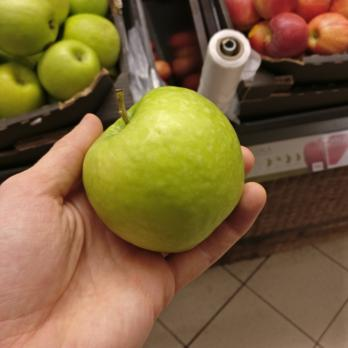
\includegraphics[width=30pt]{Chapter1/pics_paperA/Granny-Smith_021.jpg}}};
				\end{scope}
				\begin{scope}[xshift=34pt]
					\node {\fbox{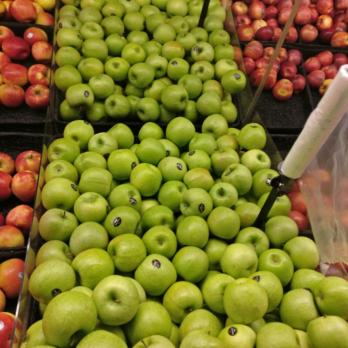
\includegraphics[width=30pt]{Chapter1/pics_paperA/Granny-Smith_012.jpg}}};
				\end{scope}
		\end{tikzpicture} }& 
		\makecell{\begin{tikzpicture}
				\begin{scope}
					\node {\fbox{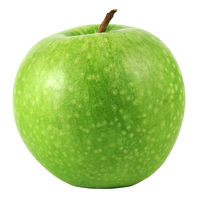
\includegraphics[width=30pt]{Chapter1/pics_paperA/Granny-Smith_Iconic.jpg}}};
				\end{scope}
		\end{tikzpicture} } & 
		\begin{scriptsize}
			\makecell{ \textit{“...\textbf{green} apple with \textbf{white, firm} pulp } \\[-1pt]  \textit{and a \textbf{clear acidity} in the flavor.”} } 
		\end{scriptsize}
		\\
		\hline 
		\makecell{ \scriptsize Tropicana \\[-1pt] \scriptsize Mandarin \\[-1pt] \scriptsize (Juice)}
		&  \makecell{ \begin{tikzpicture}
				\begin{scope}
					\node {\fbox{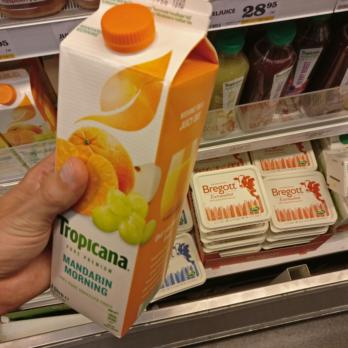
\includegraphics[width=30pt]{Chapter1/pics_paperA/Tropicana-Mandarin-Morning_003.jpg}}};
				\end{scope}
				\begin{scope}[xshift=34pt]
					\node {\fbox{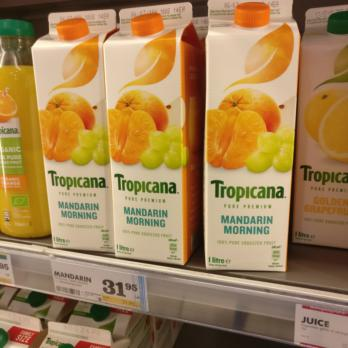
\includegraphics[width=30pt]{Chapter1/pics_paperA/Tropicana-Mandarin-Morning_016.jpg}}};
				\end{scope}
		\end{tikzpicture} }& 
		\makecell{\begin{tikzpicture}
				\begin{scope}
					\node {\fbox{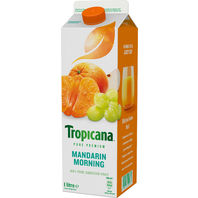
\includegraphics[width=30pt]{Chapter1/pics_paperA/Tropicana-Mandarin-Morning_Iconic.jpg}}};
				\end{scope}
		\end{tikzpicture} } & 
		\begin{scriptsize}
			\makecell{ \textit{“…is a \textbf{ready to drink} juice} \\[-1pt]
				\textit{\textbf{without pulp} pressed on \textbf{orange},} \\[-1pt]
				\textit{ \textbf{mandarin} and \textbf{grapes}. Not from} \\[-1pt]
				\textit{concentrate. Mildly \textbf{pasteurized}.” } }
		\end{scriptsize}
		\\
		\hline
	\end{tabular}
	%}
	\label{tab:paperA}
	\vspace{-3mm}
\end{table}




\begin{enumerate}
	\item[] \textbf{Marcus Klasson}, Cheng Zhang, Hedvig Kjellström. In \textit{IEEE Winter Conference on Applications of Computer Vision (WACV) 2019}.
\end{enumerate}

\paragraph{Summary}
We collect a dataset with natural images of raw and refrigerated grocery items taken in grocery stores in Stockholm, Sweden, for evaluating image classification models on a challenging real-world scenario. The data collection was performed by taking photos of groceries with a mobile phone to simulate a scenario of grocery shopping using an assistive vision app. Furthermore, we downloaded iconic images and text descriptions of each grocery item by web-scraping a grocery store website to enhance the dataset with information describing the semantics of each individual item. The items are grouped based on their type, e.g., apple, juice, etc., to provide the dataset with a hierarchical labeling structure. We show two examples of grocery item classes and their corresponding web-scraped information in Table \ref{tab:paperA}. 

We provide benchmark results evaluated using pre-trained and fine-tuned CNNs for image classification. Moreover, we take an initial step towards utilizing the rich product information in the dataset by training the classifiers with representations where both natural and iconic images have been combined through a multi-view VAE. 


\paragraph{Author Contributions}
CZ and HK presented the idea and the data collection procedure for the natural images and web-scraped information. MK performed the data collection including visiting the grocery stores for taking the natural images and the web-scraping of the grocery store website for iconic images and text descriptions. MK performed all the experiments. All authors contributed to discussing the results and contributed to writing the manuscript. 


\subsection{\underline{Paper B}: Using Variational Multi-View Learning for Classification of Grocery Items}
\label{sec:paperB}

\begin{comment}
	

\begin{figure}[t]
	\centering
	\begin{subfigure}[b]{0.3\textwidth}
		\centering
		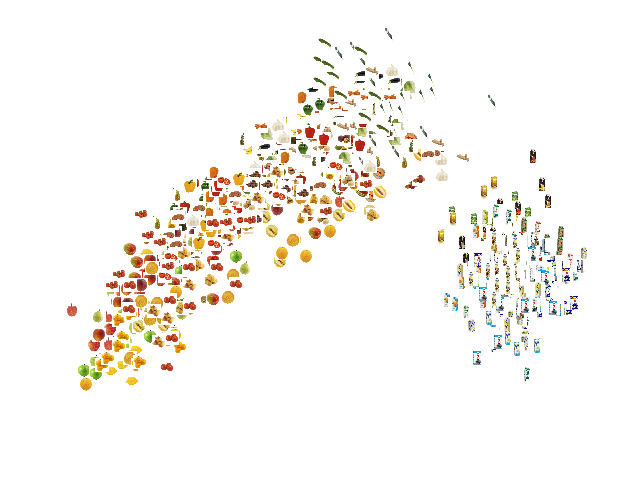
\includegraphics[width=\textwidth]{Chapter1/pics_paperB/pca_latents_vae_seed2}
		\vspace{-7mm}
		\caption{VAE$_{\vx}$}
		\label{fig:pca_latents_vae}
	\end{subfigure} 
	\hspace{-5mm}
	%\hfill
	\begin{subfigure}[b]{0.3\textwidth}
		\centering
		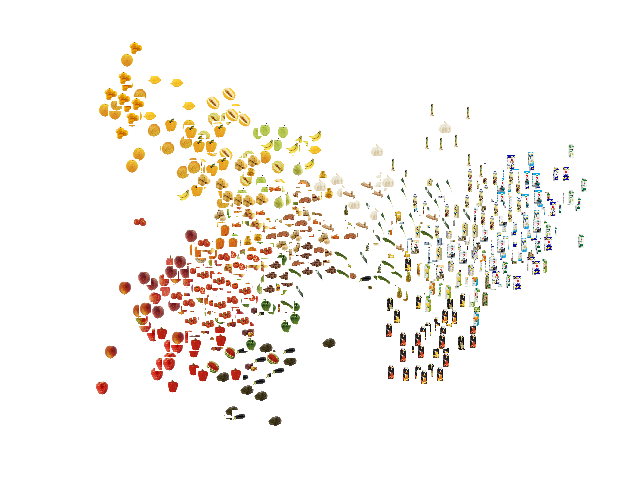
\includegraphics[width=\textwidth]{Chapter1/pics_paperB/pca_latents_vcca_xiwy_seed2}
		\vspace{-7mm}
		\caption{VCCA$_{\vx \vi \vw \vy}$ }
		\label{fig:pca_latents_vcca_xiwy}
	\end{subfigure}
	\vspace{-2mm}
	\captionsetup{width=.56\textwidth}
	\caption{Visualizations of the latent representations projected in 2D space with PCA from models VAE$_{\vx}$ and VCCA$_{\vx \vi \vw \vy}$. We plot the corresponding iconic image for each latent representation for visualization purposes. We observe that VCCA$_{\vx \vi \vw \vy}$ structures the items based on visual similarities by incorporating the web-scraped information into the latent representations, while VAE$_{\vx}$ only manages to separate the items into two clusters of raw and packaged items. }
	\label{fig:paperB_pca_latents}
\end{figure}
\end{comment}

%Visualizations of the latent representations from the test set, where we plot the iconic image of the corresponding object classes. We also plot the PCA projection of the natural image features from the off-the-shelf DenseNet169 in Figure \ref{fig:pca_densenet}. All models have been initialized with the same random seed before training. Abbreviations: VAE, Variational Autoencoder; VCCA, Variational Canonical Correlation Analysis.

%Visualizations of the latent representations $\mu_{z}$ of the red and green apples in the Grocery Store dataset. The red points correspond to the red apple classes, while the green points correspond to the green apple. The blue points correspond to the other grocery items. Abbreviations: VCCA, Variational Canonical Correlation Analysis.

\begin{enumerate}
	\item[] \textbf{Marcus Klasson}, Cheng Zhang, Hedvig Kjellström. In \textit{Patterns, Volume 1(8) (2020)}.
\end{enumerate}

\paragraph{Summary} 
We investigate whether training image classifiers can benefit from learning joint representations of grocery items using multi-view learning over the natural images and web-scraped information of the grocery items in the Grocery Store dataset (see Paper \ref{sec:paperA}). We employ a deep multi-view model based on VAEs called Variational Canonical Correlation Analysis (VCCA)~\cite{wang2016deep} for learning joint representations of the different data types, i.e., natural images, iconic images, and text descriptions. We performed a thorough ablation study over all data types to demonstrate how they contribute individually to enhancing the classification performance. Furthermore, we apply two classification approaches where we (i) train the classifier on the joint latent representations, and (ii) using a generative classifier by incorporating a class decoder to the VCCA model that can be used for classifying images. 

\begin{wrapfigure}[14]{r}[-4mm]{0.5\textwidth}
	\centering
	\vspace{-5mm}
	\begin{subfigure}[b]{0.26\textwidth}
		\centering
		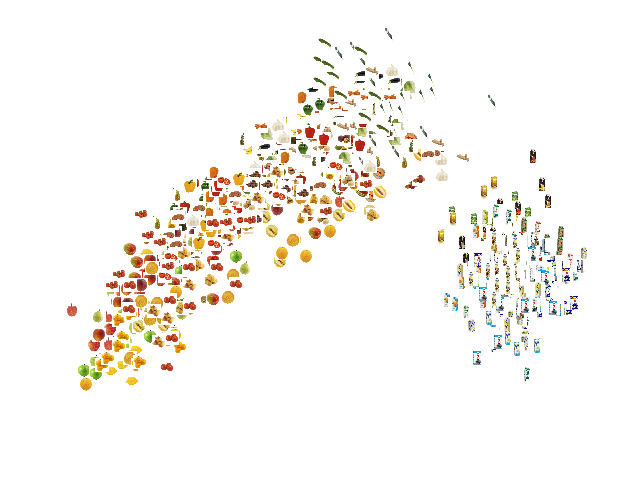
\includegraphics[width=\textwidth]{Chapter1/pics_paperB/pca_latents_vae_seed2}
		\vspace{-7mm}
		\caption{VAE$_{\vx}$}
		\label{fig:pca_latents_vae}
	\end{subfigure} 
	\hspace{-5mm}
	%\hfill
	\begin{subfigure}[b]{0.26\textwidth}
		\centering
		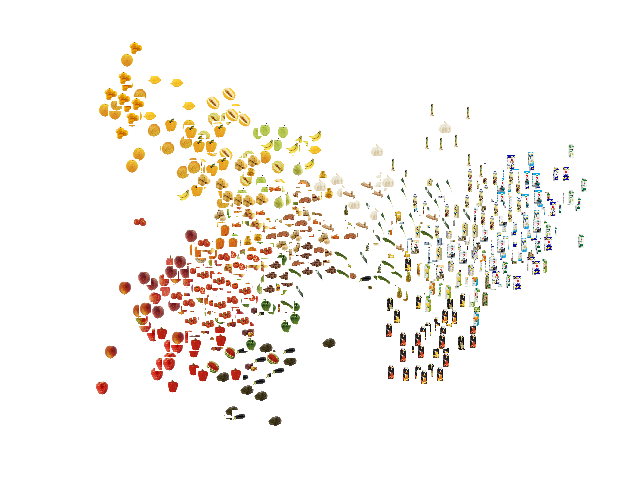
\includegraphics[width=\textwidth]{Chapter1/pics_paperB/pca_latents_vcca_xiwy_seed2}
		\vspace{-7mm}
		\caption{VCCA$_{\vx \vi \vw \vy}$ }
		\label{fig:pca_latents_vcca_xiwy}
	\end{subfigure}
	\vspace{-6mm}
	\captionsetup{width=.46\textwidth}
	\caption{Visualizations of the latent representations projected in 2D space with PCA from models VAE$_{\vx}$ and VCCA$_{\vx \vi \vw \vy}$, where we plot the corresponding iconic image for each latent representation. 
	%for visualization purposes. 
	We observe that VCCA$_{\vx \vi \vw \vy}$ structures the items based on visual similarities by incorporating the web-scraped information into the learning. 
	%We observe that VCCA$_{\vx \vi \vw \vy}$ structures the items based on visual similarities by incorporating the web-scraped information into the latent representations, while VAE$_{\vx}$ only manages to separate the items into two clusters of raw and packaged items. 
	}
	%\vspace{-3mm}
	\label{fig:paperB_pca_latents}
\end{wrapfigure} 
We performed a thorough ablation study over all data types to demonstrate how they contribute individually to enhancing the classification performance. To gain further insights into our results, we visualized the learned representations of the grocery items from VCCA and discussed how the iconic images and text descriptions help the model to better distinguish between the groceries. Our results show that the iconic images help to group the items based on their color and shape while text descriptions separate the items based on differences in ingredients and flavor. Figure \ref{fig:paperB_pca_latents} shows visualizations of the latent representations projected in 2-dimensional space using Principal Component Analysis (PCA), where we illustrate how the latents change when adding the iconic image and text description into the VCCA model. Finally, we concluded that utilizing the iconic images and text descriptions yielded better classification results than only using natural images. 


\paragraph{Author Contributions} 
CZ and HK presented the idea and all authors contributed to formalizing the methodology. 
MK performed all the experiments and created the visualizations. 
All authors took part in discussing the results.
All authors contributed to writing the manuscript. 


\subsection{\underline{Paper C}: Learn the Time to Learn: Replay Scheduling for Continual Learning}
\label{sec:paperC}

\begin{figure}[h]
	\centering 
	\includegraphics[width=0.33\textwidth]{example-image-c}
	\caption{ \MK{Paper C could illustrate the new CL setup with a figure that shows a network and a scheduler that needs to fetch a small replay memory from a huge pool of historical data.}}
	\label{fig:paperC}
\end{figure}

\begin{enumerate}
	\item[] \textbf{Marcus Klasson}, Hedvig Kjellström, Cheng Zhang. Submitted to \textit{International Conference on Machine Learning (ICML) 2022}.
\end{enumerate}

\paragraph{Summary}
In this paper, we show that learning the time to replay different tasks can be critical for continual learning (CL) performance in replay-based methods. As the main assumption in replay-based CL is that only a small set of historical data can be re-visited for mitigating catastrophic forgetting, most works have focused on improving the sample quality of the replay memory. However, in many real-world applications, historical data is accessible at all times, e.g., by storing it on the cloud. But although all historical data could be stored, retraining machine learning systems on a daily basis is prohibitive due to processing times and operational costs. Therefore, small replay memories are still needed in CL to mitigate catastrophic forgetting when learning new tasks. To this end, we propose to learn the time to learn for a CL system, in which we learn schedules over which tasks to replay at different times. Inspired by human learning, we demonstrate that scheduling over the time to replay is critical to the final CL performance with finite memory resources. We then illustrate our idea with scheduling over which tasks to replay by learning such policy with Monte Carlo tree search. We perform extensive evaluation showing that learning replay schedules can significantly improve the performance compared to baselines without learned scheduling. We also show that our method can be combined with any replay-based method and memory selection technique. Finally, our results indicate that the learned schedules are also consistent with human learning insights.



\paragraph{Author Contributions} 
CZ presented the idea and MK and CZ contributed to formalizing the methodology. 
MK performed all the experiments. 
All authors took part in discussing the results and contributed to writing the manuscript. 


\subsection{\underline{Paper D}: Meta Policy Learning for Replay Scheduling in Continual Learning}
\label{sec:paperD}

\begin{figure}[h]
	\centering 
	\includegraphics[width=0.33\textwidth]{example-image-golden}
	\caption{ \MK{Paper D could show illustration of the RL agent scheduler that gets performance measures as input and outputs an action proportion of how to select the replay memory. RL agent could also have a replay buffer where data is collected from several environments. Maybe it can also show the test case, so that it would be two separated "at training/test phase". }}
	\label{fig:paperD}
\end{figure}

\begin{enumerate}
	\item[] \textbf{Marcus Klasson}, Hedvig Kjellström, Cheng Zhang. Under preparation for conference submission.
\end{enumerate}



\paragraph{Summary} 
In this paper, we propose a reinforcement learning-based method for learning policies for replay scheduling that can be applied in new continual learning scenarios. We demonstrated in Paper C that learning the time to replay different tasks is important in continual learning. However, a replay scheduling policy that can be applied in any continual learning scenario is currently absent, which makes replay scheduling infeasible in real-world scenarios. To this end, we propose using reinforcement learning to enable learning general policies that can generalize across different data domains. 
The learned policy can then propose replay schedule that efficiently mitigate catastrophic forgetting to improve the continual learning performance without any additional computational cost in the new domain. We compare the learned policies to several replay scheduling baselines and show that the learned policies can improve the continual learning performance given task orders and datasets unseen during training. 


\paragraph{Author Contributions} 
CZ presented the idea and MK and CZ contributed to formalizing the methodology. 
MK performed all the experiments. 
All authors took part in discussing the results and contributed to writing the manuscript. 



% Thesis outline
\section{Thesis Outline}\label{sec:outline}
The rest of the thesis is organized as follows. We provide some background and preliminaries on the machine learning methodology used in this thesis in Chapter \ref{chap:background}. Chapter \ref{chap:finegrained_classification} is focused on our contributions in fine-grained classification where we first describe the related work in this field followed by explaining the frameworks used in our work. Similarly, in Chapter 4, we focus on our contributions in continual learning by first describing the related work to place our contributions in context and then describing the framework we used for enabling replay scheduling in continual learning. Finally, in Chapter 5, we provide our conclusions of the presented works and present some research directions that we believe would be interesting to look deeper into in the future. 

\MK{todo: fix references to chapters!}
%*******************************************************************************
%*********************************** Second Chapter ****************************
%*******************************************************************************

\chapter{Background}
\label{chap:background}

The goal with this chapter is to provide the reader with preliminaries that are useful for comprehending the included papers. We assume that the reader has some knowledge in calculus, linear algebra, and probability theory, but we intend to keep it on a basic level. First, we give the notation that will be used throughout the thesis. Then, we will introduce a selection of related works to place the thesis into context. 

\section{Notation and Terminology}\label{sec:notation}

We will begin by providing some algebraic notation that will be used for representing various types of data in the thesis. Scalars (both integer and real) are denoted by italic letters such as $a$. Vectors are denoted by lowercase bold italic letters such as $\vx$, where all vectors are assumed to be column vectors. A superscript $T$ denotes the transpose of a vector or matrix, such that $\vx^{T}$ becomes a row vector. Matrices are denoted as uppercase bold italic letters such as $\mW$. The notation $(w_1, \dots, w_m)$ denotes a row vector with $m$ elements, where the corresponding column vector is denoted as $(w_1, \dots, w_m)^{T}$. 

A dataset is denoted by the set $\gD = \{\vx^{(1)}, \dots, \vx^{(N)} \}$, where $\vx^{(i)}$ is the $i$-th example among the $N$ data points. Each data point is assumed to belong in a space of vectors denoted by $\gX$, such that $\vx \in \gX$. The data generating distribution is denoted by $p_{data}(\gX)$ which is usually unknown. To provide an example, we let the vector $\vx = (x_1, \dots, x_m)$ represent a flattened image of $m$ pixels. In this case, all possible images that can exist belong to the space $\gX$ and the data generating distribution $p_{data}(\gX)$ gives the probability of how likely each image is to occur in the world. In supervised learning, there is also a target, either denoted as $y^{(i)}$ or $\vy^{(i)}$, associated with $\vx^{(i)}$. The target belongs to the target space $\gY$, where the space is discrete $\gY = \{1, \dots, C\}$ for classification tasks over $C$ number of classes, or continuous $\gY = (-\infty, \infty)$ over an interval of real values for regression tasks. 

%Perhaps can skip spaces and use $\vy \in \{1, \dots, C\}$ to represent the labels and $\vx \in \mathbb{R}$, since I don't really use $\gX$ anywhere but in the RL part for state and action spaces but perhaps it's good to introduce the space notation then...

Throughout this thesis, we take a machine learning approach to solve tasks by tuning an adaptive model using a dataset called the \textit{training set}. In our case, we will represent the model with a function $f_{\vtheta}(\vx)$ that allows us to predict outcomes of events/data $\vx$ from the task of interest. The parameters $\vtheta$ expresses the function and we use machine learning algorithms for tuning parameters with the given dataset during the training phase. Once the model is trained, we often enter the \textit{test phase} where we want to evaluate the model by predicting outcomes on an unseen dataset called the \textit{test set}. The ability to predict outcomes of new data that is different from the examples seen during training is called \textit{generalization}, which is a central goal for most applications in machine learning and pattern recognition. 


\section{Problem Settings in Machine Learning}

Machine learning problems can be divided into three main fields, namely, \textit{supervised learning}, \textit{unsupervised learning}, and \textit{reinforcement learning} (RL). Since this thesis includes work from each of these problem settings, we will briefly introduce these topics to provide the reader with context on the tasks that we are trying to solve. 

\MK{TO-DO: Add references to papers and sections!}
\paragraph{Supervised Learning.} In this setting, we are given a dataset $\{(\vx^{(i)}, \vy^{(i)})\}_{i=1}^{N}$ where each data example $\vx^{(i)}$ is accompanied with a target $\vy^{(i)}$. The goal is to estimate a function $f_{\vtheta}(\vx)$ that assigns the correct target to each example in the training set as accurately as possible. In classification problems, each target belongs to one of $K$ discrete categories, such that $\vy = \{1, \dots, K\}$, and we want to predict which of the categories that new data belongs to. Classification tasks will be involved in all included papers of this thesis wherein Paper \ref{chap:paperA} and B we focus on assigning the correct product category to images of grocery items. Another problem type in supervised learning is regression where the targets are continuous and real-valued. An example of a regression task is to predict the outdoors temperature tomorrow given the observed temperature today. 

\paragraph{Unsupervised Learning.} Here, we are given a dataset $\{\vx^{(i)}\}_{i=1}^{N}$ without access to any corresponding targets. The goal in this unsupervised setting may then be to find hidden structures in the given dataset. For example, we might be interested in discovering groups of similar examples with \textit{clustering} techniques, or we may want to use \textit{density estimation} where we approximate the true data distribution $p_{data}$ with a parametric distribution $p_{\vtheta}$ using the collected dataset, or we may want to project high-dimensional data into two or three dimensions for \textit{visualization} purposes. We will get back to these goals when we introduce representation learning in Section X. 

\paragraph{Reinforcement Learning.} For these problems, we have a \textit{learning agent} that wants reach a goal in an environment by performing a given set of actions. After performing an action, the agent observes the state of the environment and receives a reward from the environment saying how good or bad the taken action was to reach the goal. The objective for the agent is to maximize the reward signal within the time the agent reaches the goal. The agent then has to learn a policy for deciding which actions to perform in certain situations in the environment. The policy $\pi_{\vtheta}(\va | \vs)$ is a mapping from perceived states $\vs$ in the environment to actions $\va$ that should maximize the reward signal. An example of a task that can be framed as a RL problem is the so called Mountain Car problem, where the agent is a car that is trying to drive up to the top of a hill. The state represents the position and velocity of the car and the agent must take actions that will move the car forward or backwards. The objective is to reach the goal with as little time as possible, and the agent is encouraged to do so by the environment by sending the agent a negative reward for every time step that passes without reaching the top of the hill. We will return to the RL framework later when we describe the prerequisites for Paper D. \vspace{1mm}

There exist many different methods for solving problems within these three fields. In this thesis, we employ deep learning methods which has been successfully applied in each field by representing the models with deep neural networks~\cite{he2016deep, bengio2013representation, mnih2015human}.

%that is trying to maximize a reward signal $r$ by performing a given set of actions in an environment to reach a specific goal. The agent observes the state of the environment 


%In this paradigm, we are concerned with decision-making where the goal is to take actions that maximize some reward. The decision-making is modeled by a policy which bases the action selection on observations that are collected by interacting with the task environment through the selected actions. One main challenge is how to handle the trade-off between exploration of different actions in new situations and exploitation by selecting actions where the agent already has experienced good reward signals. Furthermore, the reward signal can be received either in dense or sparse forms, where sparse rewards are typically more challenging to learn from and are less sample-efficient. 


\section{Deep Learning}

In this section, we give a brief overview of deep learning~\cite{goodfellow2016deep} which is the main building block for the models we use in this thesis. Deep learning contains a family of machine learning models based on neural networks that are parametric function approximators used for representing some function of interest. Much of the successes of deep learning methods have been in supervised learning settings, especially in applications where there are large amounts of labelled data and sufficiently large model in terms of number of parameters in the network. In the following sections, we will introduce the deep learning frameworks and models that we have used in this thesis.   

%For many applications, neural networks have been shown to  that are used for representing functions  are parametric function approximators. 

\subsection{Deep Neural Networks}

Neural networks is a class of machine learning models which popularity have grown immensely due to their ability to learn from large and high-dimensional datasets. Moreover, neural networks have been successfully applied in various number of fields in computer vision~\cite{he2016deep, krizhevsky2012imagenet}, natural language processing~\cite{devlin2018bert}, and reinforcement learning~\cite{mnih2015human, silver2016mastering}. These models are constructed by stacking layers of parameters that extract intermediate representations of the input data. The last layer outputs the target answer from the queried input and is specific for the task. For example, in image classification, the last layer outputs class scores representing which class the image is most likely to belong to. 

Next, we will describe three popular types of neural networks, namely, multilayer perceptrons (MLPs), convolutional neural networks (CNNs), and recurrent neural networks (RNNs). \MK{TO-DO: It would be nice to have some simple illustrations of how the networks process the data, I can take inspiration from how other people have done it.}

\paragraph{Multilayer Perceptrons.} The simplest form of feedforward neural networks is the MLP. Let the vector $\vx = (x_1, \dots, x_d)^{T}$ be some form of data where $x_i$ is the $i$-th feature for $i = 1, \dots, d$. Every layer in the MLP constitutes of weights $\mW$ that are used for transforming the input such that the output reveals some hidden structure useful for solving the task of interest. The transformation is performed with a matrix multiplication, i.e., $\vh = \mW \vx$, to receive the intermediate representation $\vh$. An essential part for enabling neural networks to learn non-linear functions is to add an activation function right after the matrix multiplication of each layer. Otherwise, the neural network would only be capable of learning linear functions since the matrix multiplication is a linear mapping. A common activation function is the $a(\vx) = \max(0, \vx)$, or the so called Rectified Linear Unit (ReLU) activation, which outputs $\vx$ when $\vx > 0$ or otherwise zero. By stacking two layers together in a neural network with a ReLU activation, we then obtain the representation $\vh = \mW_2\max(0,  \mW_1\vx)$. Note here that this representation could be predicted class scores, such that $\vh = \hat{\vy}$, if we would use two-layer MLP for a classication task. 

\paragraph{Convolutional Neural Networks.} For data where the spatial order of each feature can be salient for prediction tasks such as image classification, we need a network that can capture relationships between features. CNNs are special kinds of neural networks that can process data with grid-like structures. Convolutional layers constitutes of a set of filters with adaptable weight parameters. To produce the output, we slide each filter across the input across the width and height of the input and compute dot products between the filter weights and the input at any position. Each filter will then produce a 2-dimensional feature map that gives the responses of that filter at every spatial position. The 2-dimensional feature maps from all filters are then stacked depth-wise to obtain the output volume. The obtained feature maps are often downsampled along their spatial dimensions using a pooling operation after the activation function. The parameter sharing in convolutional layers where each weight in a filter is applied to every position of the input comes from the idea that if some visual features are important in one part of the image, it should intuitively be useful at some other location as well. Furthermore, this design choice also makes the model require fewer parameters and a lower number of operations to compute the outputs.

%Intuitively, the network will learn filters that activate when they see some type of visual feature such as edges in early layers, and eventually object parts in later layers that are discriminative . 

%Convolutional layers provide three important properties that can help the model, namely, sparse interactions, parameter sharing, and equivariant representations~\cite{goodfellow2016deep}. In MLPs, the matrix multiplication makes every output unit interact with every input unit. In contrast, CNNs typically establishes sparse interactions between the output and input by making the filter smaller than the input. This means that the model needs fewer parameters and fewer number of operations to compute the output. Furthermore, each weight is applied to every position of the input (except perhaps boundary pixels depending design choices of the layer) compared to in MLPs where a weight is multiplied with one element and never revisited.   

%An intuitive example is to detect edges in an image with pixels around local region rather than using pixels 

%Each filter operates on local regions of the input by computing the dot product between the weights and the local input region. The output is a feature map obtained by computing the dot product between the weights and the input by sliding the filter weights across the whole input.  same weights are slid across the whole input to obtain a feature map weights in a filter , where the dot product of the  

%, we The MLP operates on each input feature individually. Hence, the order of the features is ignored. However, in images, we know that pixels can have strong relationships between each other where, for instance, two neighboring pixels often have similar color and may belong to the same object that we wish to recognize. 


\paragraph{Recurrent Neural Networks.} RNNs are a family of neural network models specialized for processing sequences of data. Similar to CNNs, these models use parameter sharing by applying the same weights across several time steps. The parameter sharing is important in RNNs as it enables the model to handle different sequence lengths as well as being capable of recognizing relevant information that can appear at different locations in the sequence. Many RNNs follow the same procedure through the equation $\vh^{(t)} = f_{\vtheta}(\vh^{(t-1)}, \vx^{(t)})$, where the RNN produces the current state $\vh^{(t)}$ by incorporating the input data $\vx^{(t)}$ at time $t$ into the previous hidden state $\vh^{(t-1)}$. Hence, the hidden state $\vh^{(t)}$ will now contain information about the whole past sequence up to time $t$. In most applications, there will be an extra output layer that reads the information from state $\vh^{(t)}$ to make predictions. An example application for RNNs is predicting the next word in a sentence given previous words, where the RNN should store the necessary information about previous words to predict the rest of the sentence. A common choice of RNN model is the Long Short-Term Memory~\cite{hochreiter1997long} (LSTM) which mitigates problems with vanishing gradients during the training phase. \vspace{1mm}

For training deep networks, \textit{loss} functions are used for measuring how well the network performs to solve the task of interest. In classification tasks, the cross-entropy loss is commonly used where the predicted class scores $\hat{\vy}$ are compared against the true target class $\vy$,
\begin{align}
	\gL_{CE}(\hat{\vy}, \vy) = -\sum_{k=1}^{K} \vy[k] \log \hat{\vy}[k],
\end{align}
where the true target vector $\vy$ uses a one-hot representation where the true class $i$ is denoted in the vector by setting the $i$-th element in $\vy$ to one, as in $\vy[i] = 1$, and zero elsewhere. 

Probably the most common optimization algorithm for deep learning is stochastic gradient descent (SGD). The model parameters are updated by first computing the gradient of the loss function with respect to the weights of the network, as in $\nabla_{\vtheta} \gL(f_{\vtheta}(\vx), \vy)$, for a single input-output pair with backpropagation~\cite{rumelhart1986learning}. We can then update the parameters with the equation 
\begin{align}\label{eq:weight_update_sgd}
	\vtheta = \vtheta - \eta \nabla_{\vtheta} \gL(f_{\vtheta}(\vx), \vy),
\end{align} 
where $\eta$ is the learning rate which is an important parameter for SGD determining how much the weights should be updated with the computed gradient. 



\subsection{Deep Autoencoders}

A common architecture type for deep learning in unsupervised learning are autoencoders for learning hidden representations of unlabeled data. Autoencoders are commonly used for dimensionality reduction of high-dimensional data, where the lower-dimensional representation can be used for classification tasks, or to visualize hidden structures in the data that are hard to reveal from the original input data. The objective of the model is to reconstruct the original input data. The network architecture is built using two networks called \textit{encoder} and \textit{decoder} with a bottleneck layer between the networks for extracting the hidden representation $\vh$. The encoder and decoder architectures can be of any neural network type, such as MLPs, CNNs, or RNNs, that fits the given dataset. The encoder is used for obtaining the hidden representation of the input data, while the decoder tries to reconstruct the original input from the obtained representation. Therefore, the idea is that the learned representation should contain the relevant information for reconstructing the data. 

Mathematically, we denote the decoder as $f_{\vtheta}$ and the encoder as $g_{\vphi}$. The encoder extracts the hidden representation $\vh = g_{\vphi}(\vx)$ from the input $\vx$, then the decoder produces a reconstruction $\hat{\vx} = f_{\vtheta}(\vh)$ from $\vh$. We train the encoder and decoder simultaneously by minimizing a reconstruction loss $\gL(f_{\vtheta}(g_{\vphi}(\vx)), \vx)$, for instance mean-squared error loss, using SGD similarly as for the feedforward networks described above. There exist various kinds of methods for improving the quality of the learned representations in autoencoders. For example, we can adjust target task by adding noise to the inputs and let the decoder reconstruct the original input from noise variants~\cite{vincent2008extracting}, or we can induce different constraints in the bottleneck layer to, for example, obtain a sparse lower-dimensional representation of the data. Next, we will introduce the variational autoencoder which originates from latent variable models. 

\subsubsection{Variational Autoencoders}

The variational autoencoder~\cite{kingma2013auto} (VAE) is a variant of autoencoders where learning is viewed from the perspective of probabilistic modeling. These models come from the family of deep generative models, where the goal is to approximate some underlying data distribution $p_{data}$ with a parametric distribution $p_{\vtheta}$ learned from a dataset $\gD \sim p_{data}$. A common approach for estimating $p_{\vtheta}$ is to use a latent variable model that infers hidden structures in the data to facilitate learning the distribution. VAEs is a deep latent variable model that uses neural networks for learning $p_{\vtheta}$ making the training scalable to large high-dimensional datasets. 

The main idea with introducing latent variables is that they should encode some semantically meaningful information about the observed data. Latent variable models are usually expressed by the joint distribution 
\begin{align}
	p_{\vtheta}(\vx, \vz) = p_{\vtheta}(\vx | \vz) p(\vz),
\end{align}
where $\vz$ denotes the latent variables and $\vx$ the observed variables that represents the observed data points. The distribution $p_{\vtheta}(\vx | \vz)$ is the likelihood of the data and $p(\vz)$ is the prior distribution for the latents. This model describes the generative process of the data $\vx$ by following the steps 1) sample the latent vector $\vz \sim p(\vz)$ from the prior, and 2) generate data point $\vx \sim p(\vx | \vz)$ from the sampled latent $\vz$. We are now interested in learning the model $p_{\vtheta}(\vx, \vz)$ that best fits a given dataset $\gD$, as well as inferring the posterior distribution $p_{\vtheta}(\vz | \vx)$ over the latent variables $\vz$ given the data $\vx$.

The overall goal with latent variable models is to maximize the marginal log-likelihood $\log p_{\vtheta}(\vx)$ given a dataset $\gD \sim p_{data}$. However, computing $p_{\vtheta}(\vx)$ by with marginalizing out the $\vz$ from the model $p_{\vtheta}(\vx) = \int p_{\vtheta}(\vx, \vz) \, d\vz$ is in general intractable due to the many settings of $\vz$ we would need to evaluate. Consequently, the posterior distribution also becomes intractable since $p_{\vtheta}(\vz | \vx) = p_{\vtheta}(\vx, \vz) / p_{\vtheta}(\vx)$ from Bayes' rule. Variational inference~\cite{zhang2018advances, blei2017variational} is a technique for enabling learning of latent variable models. The idea of variational inference is to provide means for calculating the marginal log-likelihood $\log p_{\vtheta}(\vx)$ by selecting a parameterized distribution $q_{\vphi}$ for approximating the true posterior distribution. In VAEs, the approximate posterior $q_{\vphi}(\vz | \vx)$ is represented as a neural network with parameters $\vphi$ that outputs the latents $\vz$ given data points $\vx$. With this approach, we can now form a lower bound on the marginal log-likelihood given by 
\begin{align}
	\log p_{\vtheta}(\vx) \geq \E_{z \sim q_{\vphi}(\vz | \vx)}[\log p_{\vtheta}(\vx | \vz)] - \KL[q_{\vphi}(\vz |  \vx) \, || \, p(\vz)] . 
\end{align}
The right-hand side is called the evidence lower bound (ELBO) and comprises of two quantities that we can evaluate to train the model. The expectation over the log-likelihood $\log p_{\vtheta}(\vx | \vz)$ can be estimated with Monte Carlo sampling. The KL divergence between $q_{\vphi}(\vz |  \vx)$ and $p(\vz)$ can be computed analytically depending on how we choose these distributions. The standard choice for the prior is to use a zero-mean unit-variance Gaussian distribution $p(\vz) = \gN(\vz; \bm{0}, \mathbf{I})$ where $\mathbf{I}$ is the identity matrix. The approximate posterior is also selected to be a Gaussian distribution $q_{\vphi}(\vz | \vx) = \gN(\vz; \vmu_{\vphi}(\vx), \text{diag}(\vsigma_{\vphi}(\vx)))$, where the encoder network parameterized by $\vphi$ outputs the the means $\vmu_{\vphi}(\vx)$ and standard deviations $\vsigma_{\vphi}(\vx)$ for the latent dimensions. The latent vector is sampled using the "reparametrization trick"~\cite{rezende2014stochastic, kingma2013auto} by computing $\vz = \vmu_{\vphi}(\vx) + \vepsilon \odot \vsigma_{\vphi}(\vx)$, where $\vepsilon \sim \gN(\bm{0}, \mathbf{I})$ and $\odot$ denotes element-wise multiplication, which enables backpropagating gradients through the sampling operation. The likelihood $p_{\vtheta}(\vx | \vz)$ is the decoder network that tries to reconstruct the original input to the encoder. The likelihood distribution depends on the type of data $\vx$ we wish to generate. If $\vx$ is a continuous variable, then we can let the decoder output Gaussian parameters for the likelihood similar as for the encoder. 

VAEs have been used in various applications for modeling images, text, and audio data, as well as when combining data from different modalities. Next, we will briefly introduce how autoencoders can be used when learning representations from multiple data types from different modalities. 



\subsubsection{Multimodal Learning using Autoencoders}

Learning representations from different types of data is a highly active research field in deep learning~\cite{baltruvsaitis2018multimodal}. Combining visual data with other modalities such as natural language and audio signals for learning more rich representations of data has been studied frequently the last decade~\cite{owens2018audio, ngiam2011multimodal, silberer2014learning, lee2020making} [Add REFs]. A common framework in such applications is to use autoencoders for incorporating information from the different data types into a single joint representation. Learning from multiple sources then opens up for capturing correspondences between the data types and obtaining better representations that can be used for downstream tasks such as classification. 

Let $\vx$ and $\vy$ originate from two different data sources but share some high-level information. For example, $\vx$ could be an image of a living room and $\vy$ is text describing the appearance of the room, where objects are located etc. Constructing a joint representation is then done by projecting both $\vx$ and $\vy$ with separate encoder networks into the same latent space. The joint multimodal representation is then passed through two separate decoder networks used for predicting the original input data individually. The advantage of multimodal autoencoders is that they can be trained end-to-end for both learning representations as well as making predictions of the used modalities. However, a major challenge is how to handle scenarios where modalities might be missing. One option is to only encode the data modality that we know will be available at both training and test phases and then establish a joint representation by decoding two both modalities~\cite{ngiam2011multimodal}.

Multimodal autoencoders have frequently been extended to deep generative models, mainly VAEs~\cite{wang2016deep, wu2018multimodal, shi2019variational, vedantam2017generative, suzuki2016joint}. These models are capable of generating new data through sampling from the latent space in addition to learning joint representations. Furthermore, they can handle missing modalities for the encoders which enables cross-modal data generation between the modalities. In Paper B [Add REF], we employ Variational Canonical Correlation Analysis (VCCA) for learning joint representations of natural images and web-scraped information of grocery items to facilitate learning image classifiers. 


\subsection{Deep Reinforcement Learning}
\MK{TO-DO: Related works for Paper D. After writing Chapter 4 on CL}

In this section, we give a brief overview to Reinforcement Learning~\cite{sutton2018reinforcement} (RL) and introduce some approaches for how to incorporate deep neural networks in RL. 

%% talk about notation, then go into DQN, actor-critic methods and PPO briefly

%  our goal will be to tune an adaptive model  


%The tasks of interest involves estimating some probability distribution from data. In classification tasks, we are given pairs $(\vx, \vy)$ of data with an associated target label and are asked to assign one of $k$ categories to input $\vx$. Hence, our goal is to estimate the conditional probability distribution $p(\vy | \vx)$ over the target label $\vy$ given the input data $\vx$. Commonly, the distribution $p_{\vtheta}(\vy | \vx)$ is parameterized by $\vtheta$. One can also write $p_{\vtheta}(\vy | \vx)$ as a function $f_{\vtheta}(\vx): \sR \rightarrow \{1, \dots, k\}$, such that $f_{\vtheta}(\vx) = p_{\vtheta}(\vy | \vx)$, where $f$ is a function that predicts target labels $\vy$ from inputs $\vx$ by performing a mapping between the input and target spaces. Our goal is to update the parameters $\vtheta$ such that they a loss function $\gL(\vtheta)$ is minimized. A typical loss for classification tasks is the cross-entropy loss which can be minimized by taking the gradient of $\gL$ w.r.t. the parameters $\vtheta$. 


%\MK{TO-DO: How to describe computing the loss and updating the parameters? Maybe the stanford CNN course has some nice explanations?}




%The goal with this thesis is to provide machine learning methods for recognizing objects from images. Machine learning is a field within Artificial Intelligence where computer programs learns from experiences how to make predictions in new situations. There are three essential parts to enable the computer to make predictions with machine learning. Firstly, we need data representing the scenarios where we have objects that we wish to predict what they are. Secondly, we need a model that learns how to make the decisions based on the provided data. Thirdly, we need a learning algorithm for fitting the model to the data we have such that good and sensible decisions can be made on future data. Machine learning has proven to be successful on various types of data, including, images and video, text, and audio, and there exists many different kinds of models and algorithms for learning decision-making from data. 

%One of the main goals with machine learning is to have models that generalize to unseen data and events. However, there are several challenges that has to be tackled to achieve this goal. The first challenge is to obtain datasets that represent the events that the model should make predictions for. Machine learning models often require vast amounts of examples to learn from, and also, the examples should be annotated with some information describing each example in order to ease the learning. But even if we have large datasets, we must have models that have the capacity of preserving the knowledge gained from the dataset. Furthermore, we must have algorithms that can train the model from the huge amount of data in computationally efficient both time- and processing-wise. Especially for visual data, it has become much cheaper to obtain vast amounts of images and videos from the internet. Occasionally, these can be annotated through search words or, alternatively, from crowdsourcing. Moreover, computational power has also become cheaper through smaller and more efficient micro-processors, semi-conductors, and cloud computing. Deep learning~\cite{goodfellow2016deep} is a class of machine learning models based on neural networks that are capable of learning from large and high-dimensional datasets due to their capacity. They are trained using an optimization algorithm called Stochastic Gradient Descent (SGD)~\cite{bottou2010large} which works well for large-scale data and can be applied on graphical processing units (GPUs) with recent machine learning programming libraries, such as TensorFlow, PyTorch, and Jax. However, deep learning still faces lots of challenges in generalization, especially when they are applied in environments that were not present in the training data, and it is still an open research problem on how to make them generalize better. 

%There are several approaches for enabling better generalization for deep learning models. A good start is to collect datasets that are similar and represent the events in the environment where the model will be deployed. Related to this, one can also collect different data types from various modalities, such as visual signals in the form of images and video as well as natural language which can be written or spoken, if these are available in the data collection process and are sensible for the task to be solved. Multimodal machine learning opens up the possibility of learning correspondences between the different data types to gain better understanding of the phenomenon of interest~\cite{baltruvsaitis2018multimodal, xu2013survey}, which can help the model to be more accurate and robust. However, in order to enhance the utility of machine learning models, they should be capable of continuously updating their knowledge as many environments where object recognition is useful are ever-changing~\cite{delange2021continual, parisi2019continual}. We should build models that can add new objects of interest to recognize as well as delete concepts that are obsolete or non-relevant. It would also be useful if we could update models with personalized objects to recognize to narrow down the scope of items to recognize for object recognizers to make the tasks easier.  

%In this chapter, we cover related works on datasets on object recognition both with image and text data in Section \ref{sec:datasets_for_object_recognition}. Next, we provide a description of machine learning, especially deep learning, models that were used in the included papers in Section \ref{sec:machine_learning} and \ref{sec:deep_learning}. In Section \ref{sec:continual_learning}, we discuss the setting of continual learning for updating the knowledge of machine learning models that is aiming to make the models capable of handling ever-changing environments as a step towards to enabling life-long learning. 

%\section{Machine Learning Basics}

%\section{Deep Learning}

%\subsection{Autoencoders}

%\section{Reinforcement Learning}

%\subsection{Monte Carlo Tree Search}

%Data -> Modeling -> Evaluation/Generalization

% Datasets for object recognition
%\section{Datasets for Object Recognition} % Visual Recognition?
\label{sec:datasets_for_object_recognition}

The increasing accessibility of large-scale image datasets have enhanced the possibility for applying machine learning in various applications for visual recognition. One of the most well-known datasets in computer vision the is Imagenet database~\cite{deng2009imagenet} introduced in 2009 which is still used for benchmarking models on large-scale image classification. Imagenet was collected through image search results from the Internet and then further assessed by crowdsourcers from Amazon Mechanical Turk to achieve higher quality of the collected images as well as labeling them. There has been several efforts to create more large-scale vision datasets, e.g., Pascal VOC~\cite{everingham2015pascal}, Microsoft COCO~\cite{lin2014microsoft}, Visual genome~\cite{krishna2017visual}, which in addition to object classes include object attributes, bounding boxes for detecting objects, and pixel-wise segmentation masks. Additionally, there exists datasets where images have been combined with text descriptions of things that are present and where they are located in relation to each other for image captioning and visual question answering tasks, e.g., Flickr30k~\cite{young2014image}, VQA~\cite{antol2015vqa}, GQA~\cite{hudson2019gqa}, and Microsoft COCO Captions~\cite{chen2015microsoft}. These publicly accessible datasets are one of the major reasons for enabling machine learning and computer vision research at a large scale which opens up for developing products that can be deployed on everyday products, such as mobile phones. 


In order to deploy machine learning models in real-world scenarios, we first need training data that are close to the occurring events specific for the application where the model will be used. 
But even if we can train a model on huge amounts of images, it is extremely challenging to provide examples that cover all possible scenario that can happen or every different shape and color an object can have. Furthermore, other circumstances such as lighting conditions, occlusions, and other objects in the surroundings of objects of interest which can be hard to control can also make the recognition performance less accurate. This is critical when training models where the user is strongly relying on the recognition performance, such as in assistive vision systems for blind or low-vision people. As many of the popular image datasets for computer vision contains images from the Internet, there can be a large gap between the training images and the images that will be seen after deployment as Internet images often have good conditions and the objects are fully visible and centered. However, when the model would be used in the real-world, the objects could be occluded or not fully visible in the image and be disturbed by objects in the background. Therefore, it can be critical for the performance and robustness of the model to train it on images that are tailored for the scenarios where it will be applied. 

There have been several attempts to build datasets with images collected by visually impaired to obtain more realistic datasets with potential scenarios. VizWiz~\cite{gurari2018vizwiz} is one of the first large-scale image datasets with mobile phone images taken by blind people where the user have asked a question about each image that are answered by crowdworkers. This dataset is very challenging as questions asked by the collectors can be unanswerable since the objects can be occluded or even out of frame. The ORBIT dataset~\cite{massiceti2021orbit} is a more recent dataset that have built a dataset of videos from blind or low-vision people of their personal items, e.g., keys, wallets, remote controls, to enable few-shot learning of personalizable object recognizers. This dataset is the first to contain video recordings which potentially can be more user friendly as this allows the user to rotate the items that could yield more accurate performance. 




% Machine Learning introduction
%\section{Machine Learning} 
\label{sec:machine_learning}

In this section, we give a brief introduction to basics in machine learning and some mathematical notation that will be used in this chapter. The overall goal is to learn some phenomena from a set of $N$ data points $X = \{\vx_1, \dots, \vx_N\}$ where $\vx_i \in \R^{D}$ has $D$ dimensions for $1 \leq i \leq N$. The learning part is referred to as the training phase where we the goal is to fit the machine learning model to the data points, or observations, $X$. The objective of the training phase is determined by what the target task is tasks that we wish to solve using the model. Next, we give a brief description of three paradigms in machine learning with different end goals depending on what we wish to explore.

\paragraph{Supervised Learning.} Many types of data have a corresponding target $\vy$ that explains the content of each data point. Cases where the target comes from a discrete number of classes and the goal is to determine which class that the data point corresponds to are called classification problem. An classic example of a classification problem is distinguishing whether there is a cat or dog in images. If the target $\vy$ is a continuous valued variable and the goal is to predict this value, then we have a regression problem, where an example can be predicting the outdoor temperature tomorrow given the current temperature. The goal for both of these problems is to learn a function $f(\vx)$ that can classify or predict the given target data as accurately as possible. 

\paragraph{Unsupervised Learning.} For some problems, we may only have the data points for our disposal where we are interested in finding some patterns in the given data. The goal in unsupervised learning problems can be to discover similar groups with clustering techniques, or estimating the distribution of the data known as density estimation. The practitioner typically needs to define some assumptions about the data, e.g., how the similarity between two data points should be measured, before we can execute the algorithm for discovering the patterns. 

\paragraph{Reinforcement Learning.} In this paradigm, we are concerned with decision-making where the goal is to take actions that maximize some reward. The decision-making is modeled by a policy which bases the action selection on observations that are collected by interacting with the task environment through the selected actions. One main challenge is how to handle the trade-off between exploration of different actions in new situations and exploitation by selecting actions where the agent already has experienced good reward signals. Furthermore, the reward signal can be received either in dense or sparse forms, where sparse rewards are typically more challenging to learn from and are less sample-efficient. 


%%%% THINKING ABOUT MOVIND DATASETS TO HERE AND STARTING WITH ML BACKGROUND

% Deep Learning introduction
%\section{Deep Learning} 
\label{sec:deep_learning}

Neural networks is a class of machine learning models which popularity have grown immensely due to their ability to learn from large and high-dimensional datasets. Moreover, neural networks have been successfully applied in various number of fields in computer vision~\cite{he2016deep, krizhevsky2012imagenet}, natural language processing~\cite{devlin2018bert}, and reinforcement learning~\cite{mnih2015human, silver2016mastering}. These models are constructed by stacking layers of parameters that extract representations of the input data until reaching the final layer that outputs the target answer from the queried input. For example, the operation for passing the input data $\vx$ through the first layer can be denoted as the matrix multiplication $\vh = \mW_1\vx$ where $\mW_1$ are the weights of the first layer. An essential part for enabling neural networks to learn more interesting non-linear functions is to add an activation function right after the matrix multiplication of each layer, otherwise the neural network would only be capable of learning linear functions. A common activation function is the $a(\vx) = \max(0, \vx)$, or the so called Rectified Linear Unit (ReLU) activation, which outputs $\vx$ when $\vx > 0$ or otherwise zero. Stacking two layers together in a neural network with such activation between then becomes $\vh = \mW_2\max(0,  \mW_1\vx)$. In classification problems, the output layer outputs the score for which class the input $\vx$ could belong to. The weight parameters $\mW_1, \mW_2$ are learned with SGD, and their gradients are derived using the chain rule and computed using backpropagation (see \cite{goodfellow2016deep} for an introduction to backpropagation).  

\MK{Feel like I would like to include some brief info on CNNs and RNNs, but just a paragraph long for each. Maybe also describe the Autoencoders a bit. }

\subsection{Variational Autoencoders}
\label{sec:variational_autoencoders}

Generative models are used for approximating a data distribution $p_{data}$ from a given set of samples $\gD$. In most cases, we parameterize the distribution with $\vtheta$ and learn the parameters from the given data by minimizing some distance metric between the estimated distribution $p_{\vtheta}$ and $p_{data}$. In deep generative models, the distribution $p_{\theta}$ is parameterized by a neural network where the parameters $\vtheta$ represent the weights and biases in the network. These models can be broadly divided into three classes of models, namely Variational Autoencoders (VAEs)~\cite{kingma2013auto}, Generative Adversarial Networks (GANs)~\cite{goodfellow2014generative}, and Normalizing Flows~\cite{rezende2015variational}. Their commonality is that they are based on latent variable models where it is assumed that the observed data is generated from some hidden process from a simpler distribution than $p_{data}$. However, which class of models to select depends on the application and the goals with the task. In this thesis, we focus on VAEs because of their capability of learning lower-dimensional representations.

A key ingredient in learning generative models is to introduce a latent variable $\vz$ where we assume that $\vz$ is related to the observed variable $\vx$ through the data generation process. We can still estimate the parameterized distribution when introducing the latent variables since
\begin{align}\label{eq:marginal_density}
	p_{\vtheta}(\vx) = \int p_{\vtheta}(\vx, \vz) \,d\vz = \int p_{\vtheta}(\vx | \vz) p(\vz) \,d\vz,
\end{align}
where we incorporate $\vz$ to obtain the joint distribution $p_{\vtheta}(\vx, \vz)$ and use the chain rule for probabilities to obtain the likelihood $p_{\vtheta}(\vx | \vz)$ and the prior distribution $p(\vz)$. The prior $p(\vz)$ is where we can define our assumption of how the underlying hidden reasons are distributed by selecting a simple and well-known distribution for this space, e.g., a Gaussian distribution. The goal with latent variable models is often to compute the posterior $p_{\vtheta}(\vz | \vx)$ over the latent variables given the data $\vx$ which can be done using Bayes' rule 
\begin{align}
	p_{\vtheta}(\vz | \vx) = \frac{p_{\vtheta}(\vx | \vz) p(\vz)}{p_{\vtheta}(\vx)}. 
\end{align}
Unfortunately, the evidence $p_{\vtheta}(\vx)$ is very hard to compute as it requires calculating the integral $\int p_{\vtheta}(\vx, \vz) \,d\vz$ over all dimensions of the latent variable space. To overcome this issue, we will propose a distribution $q_{\vz}$ that should approximate the true posterior $p_{\vtheta}(\vz | \vx)$. Variational Inference (VI)~\cite{blei2017variational, zhang2018advances} is a method for approximating probability densities through optimization which is used in VAEs for approximating the posterior. Next, we give a description of how the posterior is approximated.
%The approximation can either be done using Markov Chain Monte Carlo (MCMC)~\cite{andrieu2003introduction} or Variational Inference (VI)~\cite{blei2017variational, zhang2018advances}. In MCMC, the idea is to use an easy-to-sample proposal distribution to draw samples that are used approximating the target distribution, while VI is a method for approximating probabilty densities through optimization. 

The learning objective in VAEs is based on the derivation of the marginal density, or evidence, in Equation \ref{eq:marginal_density}. As the evidence is intractable to compute exactly, we will instead maximize a lower bound on the evidence that is called the Evidence Lower BOund (ELBO). The ELBO is derived in log-space such that we can apply Jensen's inequality to obtain the lower bound when we have introduced the approximate posterior $q_{\vphi}(\vz | \vx)$ parameterized by $\vphi$. We begin be deriving a general expression for the ELBO: 
\begin{align}\label{eq:elbo}
	\begin{split}
		\log p_{\vtheta}(\vx) & = \log \int p_{\vtheta}(\vx, \vz) \,d\vz \\ 
		& = \log \int \frac{q_{\vphi}(\vz | \vx) p_{\vtheta}(\vx , \vz)}{q_{\vphi}(\vz | \vx)} \,d\vz \\
		& = \log \E_{q_{\vphi}(\vz | \vx)}\left[ \frac{p_{\vtheta}(\vx , \vz)}{q_{\vphi}(\vz | \vx)}\right] \\
		& \geq \E_{q_{\vphi}(\vz | \vx)}\left[ \log \frac{p_{\vtheta}(\vx , \vz)}{q_{\vphi}(\vz | \vx)}\right] ,
	\end{split}
\end{align}
where we applied Jensen's inequality between the third and fourth line to obtain the ELBO. This expression can be derived further to obtain the common VAE objective
\begin{align}\label{eq:vae}
	\begin{split}
		\log p_{\vtheta}(\vx) & \geq \E_{q_{\vphi}(\vz | \vx)}\left[ \log \frac{p_{\vtheta}(\vx , \vz)}{q_{\vphi}(\vz | \vx)}\right] \\
		& = \E_{q_{\vphi}(\vz | \vx)}\left[ \log p_{\vtheta}(\vx | \vz) \right] - \KL[q_{\vphi}(\vz | \vx) \,||\, p(\vz)], 
	\end{split}
\end{align}
where the second term is the Kullback-Leibler (KL) divergence between the approximate posterior and the prior. The KL divergence can be computed exactly when selecting both $q_{\vphi}(\vz | \vx)$ and $p(\vz)$ to be Gaussian densities, while the expectation of the log-likelihood can be estimated with Monte Carlo approximation. Furthermore, the reparameterization trick~\cite{kingma2013auto, rezende2014stochastic} is used to enable computing the gradients through the sampling step when estimating the log-likelihood that can be used for backpropagation. 


\subsection{Multi-View Learning}

Humans make use of many different sensory signals to recognize objects in the world. Visual signals are rich in the sense they convey the identity of objects. But even without vision capabilities, we can use touch, smell, and sound to ease the recognition problem of a near item, or even text for describing the features of objects. Combining each of these signals should help us obtain better recognition performance as we are adding information. This is a popular approach in machine learning to improve the recognition performance by utilizing various \textit{modalities} and \textit{views}. The difference between a modality and a view is that modalities refers to the way in which something happens or is experienced~\cite{baltruvsaitis2018multimodal}, e.g., natural language that can be written or spoken and visual signals in the form of images and videos, while views can be broadly defined as any sensor stream of a scene or event~\cite{salzmann2010factorized}. Example of views can be images taken from different camera view points or different environments, as long as the camera sensors are different. Another example are written or spoken languages where each language is considered its own view. In the rest of this section, even if they are very similar, we will discuss multi-view learning rather than multimodal learning as we utilize images from two different views in Paper \ref{sec:paperB} when training classifiers. 
\MK{Add figure with examples of what a view is, I can take inspiration from Fig 1 in C. Xu Survey on MVL. }

Multi-view learning 







% Continual Learning introduction
%\section{Continual Learning in Neural Networks}
\label{sec:continual_learning}

A common assumption in machine learning is that the data comes from stationary distributions such that the properties of the data are the same over time. However, this assumption may complicate deployments in real-world applications where variations in the data is common and the data seen during deployment can be very different from the data used for training. Such models has to be capable of learning from experiences online and update its knowledge about new concepts that are encountered during the lifespan. Furthermore, as the model is operating in an online manner, the model has to adapt fast when learning new knowledge to minimize the time that the system has to be down during training. These requirements has lead to research in Continual Learning (CL)~\cite{delange2021continual, parisi2019continual} where the goal is to push neural networks closer to how humans and animals are learning various tasks during their lifespan.

Next, we introduce some notation of the problem setting in CL for image classification. We let a neural network $f_{\vtheta}$, parameterized by $\vtheta$, learn $T$ tasks sequentially given their corresponding task datasets $\gD_1, \dots, \gD_T$ arriving in order. The $t$-th dataset $\gD_t = \{(\vx_{t}^{(i)}, y_{t}^{(i)})\}_{i=1}^{N_{t}}$ consists of $N_t$ samples where $\vx_{t}^{(i)}$ and $y_{t}^{(i)}$ are the $i$-th data point and class label respectively. The training objective at task $t$ is given by 
\begin{align}
	\underset{\vtheta}{\text{min}} \sum_{i=1}^{N_t} \ell(f_{\vtheta}(\vx_t^{(i)}), y_{t}^{(i)}),
\end{align}
where $\ell(\cdot)$ is the loss function, e.g., cross-entropy loss in image classification problems. Since $\gD_t$ is only accessible at time step $t$, the network $f_{\vtheta}$ is at risk of \textit{catastrophically forgetting} the previous $t-1$ tasks when learning the current task. 
%Replay-based continual learning methods mitigate the forgetting of old tasks by storing old examples in an external replay memory, that is mixed with the current task dataset during training. Next, we describe our method for constructing this replay memory.  

There are several desired properties of CL systems mentioned in~\cite{schwarz2018progress} to enhance their utility. Firstly, they should be capable of retaining already existing knowledge to mitigate the catastrophic forgetting effect that neural networks are susceptible to when trained in CL settings. Secondly, we hope that the model can benefit from the previously learned tasks to ease the learning of new tasks, which is referred to as \textit{forward transfer}. Moreover, we wish that learning new tasks can have positive influence on the performance of old tasks which is called \textit{backward transfer}. It also needs to be \textit{scalable} to a large number of tasks that could be encountered during its life time. Finally, it should ideally be capable of learning without the need for task labels as there might be unclear task boundaries when the model is deployed. 

Research in CL can be divided into three main areas, namely regularization-based, architecture-based, and replay-based approaches. Regularization-based methods aim to mitigate catastrophic forgetting by protecting parameters influencing the predictive performance from wide changes and use the rest of the parameters for learning the new tasks~\cite{adel2019continual, chaudhry2018riemannian, kirkpatrick2017overcoming, li2017learning, nguyen2017variational, rannen2017encoder, schwarz2018progress, zenke2017continual}. Architecture-based methods isolate task-specific parameters by either increasing network capacity~\cite{rusu2016progressive, yoon2019scalable, yoon2017lifelong} or freezing parts of the network~\cite{mallya2018packnet, serra2018overcoming} to maintain good performance on previous tasks. 
Replay-based methods mix samples from old tasks with the current dataset to mitigate catastrophic forgetting, where the replay samples are either stored in an external memory~\cite{chaudhry2019tiny, hayes2020remind, isele2018selective, lopez2017gradient} or generated using a generative model~\cite{shin2017continual, van2018generative}. More recently, there has been work on compressing raw images to feature representations to increase the number of memory examples for replay~\cite{hayes2020remind, iscen2020memory, pellegrini2019latent} as well as applying ideas from contrastive learning to improve retaining past knowledge~\cite{cha2021co2l, mai2021supervised}. 
Regularization-based approaches and dynamic architectures have been combined with replay-based approaches to methods to overcome their limitations~\cite{chaudhry2018riemannian, chaudhry2018efficient, douillard2020podnet, ebrahimi2020adversarial, joseph2020meta, mirzadeh2020linear, nguyen2017variational, pan2020continual, pellegrini2019latent, rolnick2018experience, von2019continual}. In general, these methods share the goal of mitigating catastrophic forgetting in various ways and then they can have additional goals related to the other desired properties on forward- and backward transfer, task scalability, and avoiding the need for task labels. 







%*******************************************************************************
%*********************************** Third Chapter *****************************
%*******************************************************************************

\chapter{Fine-grained Classification}
\label{chap:finegrained_classification}

%% Write about Paper A and B in a coherent way

This chapter presents an approach for enhancing fine-grained classification performance of grocery items by using web-scraped information. We focus on classification of grocery items due to applicability in assistive vision and its potential to enhance the independence of visually impaired (VI) people [ADD groceries/shopping/object recognition for VI REFs]. Initially, we were interested in learning classifiers with natural images taken in the grocery stores combined with web-scraped information about the grocery items, such as iconic images and text descriptions from supermarket websites. Using iconic images have been used in grocery image classification earlier [ADD grocery paper REFs], however, utilizing text descriptions was as far we know absent for this application even if it has been successfully applied in other image classification problems [ADD REFs, Bujwid and Sullivan, AwA dataset, or other Attribute datasets]. Thus, we collected our own dataset of grocery items images using a mobile phone camera as well as web-scraped images and text descriptions to study whether this multi-view approaches would benefit training the classifiers (Section 2). We then select a multi-view learning framework based on the Variational Autoender (VAE) for investigating how the different data views affect the fine-grained classification performance (Section 3). 

%\section{Introduction}
\section{Related Work}
\section{Dataset Collection}
\section{Representation Learning}
\section{Experiments}
\section{Discussion}


\noindent 
%In this chapter, we provide a summaries of the included paper for this thesis. Paper \ref{sec:paperA} and \ref{sec:paperB} are connected through the Grocery Store dataset where we present the work and then perform an ablation study over which modalities in the dataset that are useful for training classifiers. In Paper \ref{sec:paperC} and \ref{sec:paperD}, we focus on continual learning (CL) and present a new setting that aims to fill the gap between CL research and real-world problems as well as a method for doing so. 

%\begingroup
%\renewcommand\thesection{\Alph{section}} % for changing section numbering to alphabetic
%
\section{A Hierarchical Grocery Store Image Dataset with Visual and Semantic Labels}
\label{sec:paperA}

\textbf{Authors:} Marcus Klasson, Cheng Zhang, Hedvig Kjellström. 

\paragraph{Summary.} 
We collect a dataset with natural images of raw and refrigerated grocery items taken in grocery stores in Stockholm, Sweden, for evaluating image classification models on a challenging real-world scenario. The data collection was performed by taking photos of groceries with a mobile phone to simulate a scenario of grocery shopping using an assistive vision app. Furthermore, we downloaded iconic images and text descriptions of each grocery item by web-scraping a grocery store website to enhance the dataset with information describing the semantics of each individual item. the items are grouped based on their type, e.g., apple, juice, etc., to provide the dataset with a hierarchical labeling structure. 

We provide benchmark results evaluated using pre-trained and fine-tuned CNNs for image classification. Moreover, we take an initial step towards utilizing the rich product information in the dataset by training the classifiers with representations where both natural and iconic images have been combined through a multi-view VAE. 



\paragraph{Author Contributions.} CZ and HK presented the idea and the data collection procedure for the natural images and web-scraped information. MK performed the data collection including visiting the grocery stores for taking the natural images and the web-scraping of the grocery store website for iconic images and text descriptions. MK performed all the experiments. All authors contributed to discussing the results and contributed to writing the manuscript. 


%
\section{Using Variational Multi-view Learning for Classification of Grocery Items}
\label{sec:paperB}

\textbf{Authors:} Marcus Klasson, Cheng Zhang, Hedvig Kjellström. 
%
\section{Learn the Time to Learn: Replay Scheduling for Continual Learning}
\label{sec:paperC}
%
\section{Meta Policy Learning for Replay Scheduling in Continual Learning}
\label{sec:paperD}

\textbf{Authors:} Marcus Klasson, Hedvig Kjellström, Cheng Zhang. 

\paragraph{Summary.} 



\paragraph{Author Contributions.} CZ presented the idea. 


%\endgroup

%*******************************************************************************
%*********************************** Fourth Chapter ****************************
%*******************************************************************************


\chapter{Continual Learning}\label{chap4}

In this chapter, we give an overview of Paper \ref{paperC} and \ref{paperD} where we focus on continual learning (CL)~\cite{delange2021continual,parisi2019continual}. A CL system receives samples of classes to learn continuously over time while maintaining its overall performance on every seen class. Such capability is critical for assistive vision systems as the system may need to adapt to unseen items in new environments. Furthermore, CL on mobile devices would enable personalizing the devices to specific items that the VI user wants to locate and recognize. 
The main challenge with the CL setup is catastrophic forgetting~\cite{mccloskey1989catastrophic} where previously learned abilities are overwritten by recent acquired knowledge (see Figure \ref{fig:catastrophic_forgetting_example}). However, retraining on all previously seen data may be prohibited due to lack of computational budget or accessibility to the seen datasets. Replay-based CL methods efficiently mitigate catastrophic forgetting by revisiting old samples stored in a small memory buffer~\cite{chaudhry2019tiny,lopez2017gradient,hayes2020remind}. 

Most replay-based methods in CL use simple strategies for retrieving replay samples and ignore the time to learn which is important for memory retention in human learning~\cite{dempster1989spacing,landauer1978optimum,hawley2008comparison}. 
Furthermore, most works rely on tiny memory buffers although historical data is almost always available in many real-world machine learning applications~\cite{mitchell1999machinelearning,bailis2017macrobase,hazelwood2018applied}. Nevertheless, the requirement of small replay memories remains as due to limitations on computational budget and data transmission times. 
To this end, we propose in Paper \ref{paperC} a new CL setting where historical data is
available while the processing time is limited. For this new setting, we propose \textit{replay scheduling} where we select which tasks to replay at different times, and demonstrate the advantages of considering time to replay in CL. 
In Paper \ref{paperD}, we present a framework based on reinforcement learning (RL)~\cite{sutton2018reinforcement} for learning replay scheduling policies that can be transferred to new CL scenarios for mitigating catastrophic forgetting without added computational cost. 
Our proposed replay scheduling approach opens up for new research directions that can bring current CL research closer to real-world needs. 


%This chapter introduces the idea of replay scheduling for mitigating catastrophic forgetting in continual learning (CL). The problem setting of CL is on learning tasks of recognizing a new set of classes with a dataset given at the current time step. In the standard setting, one main assumption is that the data from past tasks can never be fully revisited by the model. However, in the real-world, many organizations record data from incoming streams for storage rather than deleting it~\cite{bailis2017macrobase, mitchell1999machinelearning} [Add at least 1 more REF]. In contrast to the assumption on data storage in standard CL, we suggest a new setting where we assume that all seen data is accessible at any time for the model to revisit. The challenge then becomes how to select which tasks that needs to be remembered via replay as the data is still incoming from a stream. We propose to learn the time when replaying a certain task is necessary when the model is updating its knowledge with new incoming tasks. In Paper \ref{paperC}, we propose the new CL setting where historical data is accessible and introduce the idea of replay scheduling and how it can be used in CL. In Paper \ref{paperD}, we propose a framework based on reinforcement learning~\cite{sutton2018reinforcement} (RL) for learning replay scheduling policies that can be applied in new CL scenarios. 

%A simple, yet effcient, approach to mitigate catastrophically forgetting past tasks is to add some 
%Replay scheduling involves selecting which tasks to fetch examples from and add to a replay memory at different times. The replay memory is then mixed with a batch of examples from the current task to learn to help the network to remember the previously learned tasks selected by the scheduler. 

%\MK{TO-DO: Motivate replay scheduling from mobile phone perspective, perhaps from perspective that phones can store lots of data but how to select which classes to replay. Maybe it should also be from the computational perspective, that we want such scheduling policy to work in many scenarios without additional compute cost for the policy learning. }

\begin{figure}[t]
	\centering
	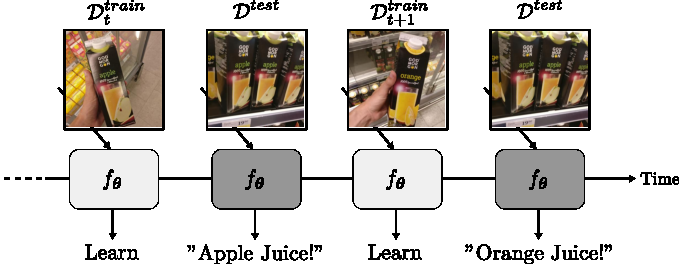
\includegraphics[width=0.8\textwidth]{Chapter4/imgs/cf_new.pdf}
	\caption{Illustration of catastrophic forgetting in a continual learning scenario. The network $f_{\vtheta}$ receives a task dataset of an Apple Juice class in $\gD_{t}^{train}$ to learn, and correctly predicts the Apple Juice class in the unseen test image in $\gD^{test}$. The next task dataset involves learning an Orange Juice class from $\gD_{t+1}^{train}$ which $f_{\vtheta}$ adapts to without retaining knowledge about the Apple Juice class, such that $f_{\vtheta}$ makes the wrong prediction during evaluation on $\gD^{test}$ again. }
	\vspace{-2mm}
	\label{fig:catastrophic_forgetting_example}
\end{figure}


\section{Related Work}\label{chap4:sec:related_work}

In this section, we give an overview of different approaches in CL, especially replay-based methods which our proposed replay scheduling approach in Paper \ref{paperC} and \ref{paperD} is based on. 

\vspace{-3mm}
\paragraph{Continual Learning.} The existing CL approaches for mitigating catastrophic forgetting in neural networks can broadly be divided into three main areas, namely, regularization-based, architecture-based, and replay-based methods. 
Regularization-based methods mainly focus on 
preventing the parameters important for previous tasks from wide changes and fit the remaining parameters to new tasks~\cite{kirkpatrick2017overcoming, zenke2017continual, nguyen2017variational}. 
Knowledge distillation methods~\cite{hinton2015distilling} also belong to these methods where stored classification logits are used for regularizing the output units for previous tasks in the network~\cite{li2017learning, schwarz2018progress}.
More recently, projection-based approaches have been proposed for constraining the parameter updates to subspaces which avoid interference with previous tasks~\cite{saha2021gradient, kao2021natural}. 
Architecture-based methods focus on adding task-specific network modules for every seen task~\cite{rusu2016progressive, yoon2017lifelong, yoon2019scalable, ebrahimi2020adversarial}, or isolating parameters for predicting specific task in fixed-size networks~\cite{mallya2018packnet, serra2018overcoming, schwarz2021powerpropagation}. 
Replay-based methods revisits samples from old tasks when learning new tasks. The old samples are either stored in an external memory~\cite{chaudhry2019tiny, hayes2020remind, rolnick2018experience,jin2020gradient,verwimp2021rehearsal}, or synthesized with a generative model~\cite{shi2019variational, van2018generative, van2020brain, wu2018memory}. 
Both regularization- and architecture-based methods can be combined with replay for improving the models capability of remembering tasks~\cite{buzzega2020dark,douillard2020podnet,ebrahimi2020adversarial,joseph2020meta,mirzadeh2020linear,nguyen2017variational,pan2020continual,von2019continual}. 
Our replay scheduling idea is originated from replay-based methods which we will cover more in detail next. 

%\paragraph{Continual Learning.} There exist many different approaches in CL for mitigating catastrophic forgetting in neural networks. In general, these approaches can be divided into three main cores, namely, \textit{regularization-based}, \textit{architecture-based}, and \textit{replay-based} methods. Regularization-based methods are mainly focused on applying regularization techniques on parameters important for recognizing old tasks and fit the remaining parameters to new tasks~\cite{kirkpatrick2017overcoming, zenke2017continual, nguyen2017variational}. Knowledge distillation methods~\cite{hinton2015distilling} also belong to these approaches where classification logits are used for regularizing the output units for previous tasks in the network~\cite{li2017learning, schwarz2018progress}. More recently, there are some works that uses projection-based approaches for constraining the parameter updates to subspaces which avoid interference with previous tasks~\cite{saha2021gradient, kao2021natural}. Architecture-based approaches focuses on adding task-specific network modules for every seen task~\cite{rusu2016progressive, yoon2017lifelong, yoon2019scalable, ebrahimi2020adversarial}, or isolating parameters for predicting specific task in fixed-size networks~\cite{mallya2018packnet, serra2018overcoming, schwarz2021powerpropagation}. Replay-based methods re-trains on samples of old tasks when learning new tasks. The old samples are either stored in an external memory~\cite{chaudhry2019tiny, hayes2020remind, rolnick2018experience}, or synthesized with a generative model~\cite{shi2019variational, van2018generative, van2020brain, wu2018memory}. Both regularization- and architecture-based methods can be combined with replay for improving the models capability of remembering tasks [Add REFs]. Our replay scheduling idea is originated from replay-based methods which we will cover more in detail next. 

\vspace{-3mm}
\paragraph{Replay-based Continual Learning.} 
Much research effort in replay-based CL has focused on selecting higher quality samples to store in memory~\cite{aljundi2019gradient, borsos2020coresets, chaudhry2019tiny, chrysakis2020online, hayes2019memory, isele2018selective, lopez2017gradient, nguyen2017variational, rebuffi2017icarl, yoon2021online}. In \cite{chaudhry2019tiny}, several selection strategies are reviewed in scenarios with tiny memory capacity, such as reservoir sampling~\cite{vitter1985random}, first-in first-out buffer~\cite{lopez2017gradient}, k-Means, and Mean-of-Features~\cite{rebuffi2017icarl}. However, elaborate selection strategies have been shown to give little benefit over random selection for image classification problems~\cite{chaudhry2018riemannian, hayes2020remind}. 
More recent work has been focused on enhancing the memory capacity by storing compressed features rather than raw data~\cite{hayes2020remind, iscen2020memory, pellegrini2019latent}, evolving the memory samples using data augmentation to avoid overfitting~\cite{jin2020gradient,bang2021rainbow}, and using contrastive learning to improve memory retention~\cite{cha2021co2l,mai2021supervised}. 
Selecting the time to replay old tasks has mostly been ignored in the literature, with an exception in~\cite{aljundi2019online} which replays memory samples that would most interfere with a foreseen parameter update. Our replay scheduling approach differs from the above mentioned works since we focus on learning to select which tasks to replay. Nevertheless, our scheduling can be combined with any selection strategy and replay-based method.


%\paragraph{Replay-based Continual Learning.} In this thesis, we focus on replay-based methods with external memories for storing historical data. The most common selection strategy for filling the memory is random sampling from the used datasets. There exist several works focusing on selecting high quality samples for storing in the memory [Add REFs]. However, in image classification problems, random sampling has been shown to often perform on par with more elaborate selection strategies~\cite{chaudhry2018riemannian, hayes2020remind}. In contrast to using various memory selection methods, there has been proposals of retrieval policies over which samples to select for replay from the memory, for instance, selecting the samples that will mostly interfere with the parameter update with batches of new data~\cite{aljundi2019online}. Our replay scheduling approach differs from this method as we focus on selecting which tasks to select for replay rather than the individual samples to retrieve from the memory. More recent works have focused on evolving the memory samples through data augmentation to avoid overfitting to the memory [Add REFs], and also by using contrastive learning to improve discriminating between tasks. Another direction has been to increasing the storage capacity to store more samples by compressing raw data into features that are more memory-cheap [Add REFs]. The above mentioned methods assume that the memory is small and allocates equal storage amount for all tasks. Our new problem setting for memory-based CL is different from this assumption as we argue that data storage is cheap in many real-world applications. Hence, we compose a replay memory with data from historical tasks before learning new tasks because the amount of compute is limited. However, replay scheduling can be combined with of the mentioned methods as it only differs with the standard memory-based CL setting in that the replay memory has to be selected at every new task. 

%\vspace{-3mm}
%\paragraph{Generalization in Reinforcement Learning.} Generalization in RL is an active research field where much focus has been put on developing proper benchmark datasets for evaluating generalization capabilities of RL agents~\cite{cobbe2019quantifying, cobbe2020leveraging, nichol2018gotta, yu2020meta}.  Regularization techniques from supervised learning have been used to investigate whether these can enhance generalization in RL~\cite{cobbe2019quantifying, farebrother2018generalization, igl2019generalization}, and also how variations in the environments help to obtain agents that generalize better~\cite{packer2018assessing, zhang2018dissection}. Algorithms for enabling fast adaptation to new environments, such as new tasks~\cite{finn2017model, kessler2021same} and new action spaces~\cite{chandak2019learning, jain2020generalization}, has also been studied. The survey by Kirk \etal~\cite{kirk2021survey} focuses on zero-shot policy transfer where the policy must generalize to unseen dynamics in the test environments as additional queries could be disallowed in real-world scenarios~\cite{yang2019single, ball2021augmented}. In Paper \ref{paperD}, we consider using RL for learning policies for scheduling which tasks to replay in CL settings to mitigate catastrophic forgetting in the classifier. The policy is trained using experiences from multiple CL environments and then tested in new CL environments with unseen dynamics such as new task orders and datasets. 
%We evaluate our learned policies on the zero-shot policy transfer setting where the goal is to mitigate catastrophic forgetting in new CL scenarios. The rewards are accessible through accuracies calculated on validation datasets, however, fine-tuning the policy during CL training is prohibited.  



% General CL papers, add new papers that you have seen. Then Replay/memory-based CL approaches, add new and contrastive approaches. Perhaps something on meta-policy learning approaches, would be useful to tell how we use reinforcement learning here

%TO-DO \MK{A short and cozy table fo this, similar to survey by Delange etal 2021}
%\paragraph{Similarities and Differences between Continual Learning and other fields.} \MK{A short and cozy table fo this, similar to survey by Delange etal 2021}


\section{Replay Scheduling in Continual Learning}\label{chap4:sec:replay_scheduling_in_cl}

In this section, we present our proposed replay scheduling approach studied in Paper \ref{paperC} and \ref{paperD} for mitigating catastrophic forgetting in CL. 
More specifically, we focus on the contributions in Paper \ref{paperC}, where we introduce a slightly new CL setting that considers real-world needs where all historical data can be available since data storage is cheap. Additionally, we demonstrate the advantages of replay scheduling in such setting where we select which tasks to replay, where we use Monte Carlo tree search (MCTS)~\cite{coulom2006efficient} to search for efficient replay schedules by allowing multiple episodes in single CL environments. 


%In this section, we introduce a slightly new CL setting considering the real-world needs where all historical data can be available since data storage is cheap. However, the amount of compute is limited when the model is updated on new data due to operational costs. Hence, it is impossible for the model to leverage from all the available historical data to mitigate catastrophic forgetting. The goal then becomes to learn how we can select subsets of historical data for replay to efficiently reduce forgetting of the old tasks. We will refer to these subsets of historical data as the \textit{replay memory} throughout this chapter. The size of the replay memory affects the processing time when learning new tasks as well as the allowed time for the training phase. When composing the replay memory, we focus on determining the number of samples to draw from the seen tasks in the historical data rather than selecting single stored instances. Next, we introduce the problem setting in more detail as well as the notation of the new CL setting. 


\subsection{New Problem Setting for Continual Learning}

In this section, we describe the proposed CL setting presented in Paper \ref{paperC}. We assume that historical data is accessible at any time for mitigating catastrophic forgetting in the model. However, re-training the model on all available historical data is prohibited due to limitations on compute and data transmission times. Therefore, the goal is to determine which historical tasks to replay and sample a small replay memory from the selected tasks to mitigate catastrophic forgetting as efficiently as possible. 

The notation of this problem setting resembles the traditional CL setting for image classification. We let a neural network $f_{\vphi}$, parameterized by $\vphi$, learn $T$ tasks from the datasets $\gD_1, \dots, \gD_T$ arriving sequentially one at a time. The $t$-th dataset $\gD_t = \{(\vx_{t}^{(i)}, y_{t}^{(i)})\}_{i=1}^{N_{t}}$ consists of $N_t$ samples where $\vx_{t}^{(i)}$ and $y_{t}^{(i)}$ are the $i$-th data point and class label respectively. Additionally, the dataset is split into training, validation, and test sets such that $\gD_{1:T} = \{(\gD_{t}^{train}, \gD_{t}^{val}, \gD_{t}^{test})\}_{t=1}^{T}$. The training objective at task $t$ is given by 
%\vspace{-2mm}
\begin{align}
	\underset{\vphi}{\text{min}} \sum_{i=1}^{N_t} \gL(f_{\vphi}(\vx_t^{(i)}), y_{t}^{(i)}),
\end{align}
where $\gL(\cdot)$ is the loss function, which in our case is the cross-entropy loss. The challenge is for the network $f_{\vphi}$ to retain its classification performance on the previous $t-1$ tasks. 

We assume that historical data from old tasks are accessible at any time step. However, we can only fill a small replay memory $\gM$ with $M$ historical samples for mitigating catastrophic forgetting of old tasks due to processing time constraints. The challenge then becomes how to select the $M$ samples from the historical data to include in the replay memory that efficiently retain the previous knowledge. 
We focus on selecting the samples on task-level by deciding on the task proportions $(p_1, \dots, p_{t-1})$ on samples to fetch from each task, where $\sum_{i=1}^{t-1} p_i = 1$ and $p_{i} \geq 0$. The number of samples from task $i$ to place in $\gM$ is given by $p_i \cdot M$. To simplify the selection of which tasks to replay, we construct a finite set of possible task proportions that can be used for constructing $\gM$. 

This problem setting shares several assumptions with traditional CL, such as:
\begin{itemize}[noitemsep,topsep=1pt]
	\item The model receives the datasets at different time steps from a continuous stream.
	\item Re-training on all historical data is prohibited.
	\item The model should perform well overall across all seen tasks and, hence, mitigate catastrophic forgetting.
	\item Replay memory size $M$ is small.
\end{itemize}
The only difference with this setting and traditional CL is that all historical has been stored rather than deleted, and we can access this data to fill the replay memory $\gM$ to mitigate catastrophic forgetting. We argue that this setting aligns well with real-world needs as data storage is cheap and easy to maintain but retraining large machine learning models is computationally expensive. Therefore, we use small replay memory sizes to limit the processing times of replay when the model is learning new tasks. 


%\paragraph{Comparison to Traditional CL.} The new setting has several similarities to the traditional CL setting. Both settings share the fundamental setting that the data arrive in streams and re-training on all historical data is prohibited. Also, the goal that the model should perform well both historical tasks and tasks associated with new data remains the same. In replay-based CL, we also share the same constraints that the memory size is limited. However, we argue that this limitation is mainly associated with compute rather than of storage. Our assumption aligns with the real-world where data storage is cheap and easy to maintain, but retraining large machine learning models is computationally expensive. The only difference is that we allow filling the limited replay memory from historical data or some other external memory. Here, we argue that historical data is stored rather than deleted in many real-world settings~\cite{bailis2017macrobase}. Thus, we should keep the limited memory assumption for training but allow access to historical data to fill the replay memory to make CL align with real-world needs.
%\MK{TO-DO: this paragraph can be written in a more humble way, more like "this is something worth to investigate"}



%\subsection{Replay Scheduling for Mitigating Catastrophic Forgetting}
\subsection{Monte Carlo Tree Search for Replay Scheduling}

In this section, we describe how we used MCTS in Paper \ref{paperC} to show the advantages of replay scheduling in the new CL setting. We focus on an ideal CL environment where executing multiple episodes is allowed to enable searching for replay schedules. For demonstration purposes, we use MCTS for finding replay schedules that efficiently mitigate catastrophic forgetting by selecting compositions of replay memories at different time steps. 

\begin{wrapfigure}{r}{0.43\textwidth}
\hspace{-4mm}
\begin{minipage}{0.43\textwidth}
\vspace{-7mm}
\begin{algorithm}[H]
	\footnotesize
	\caption{Discretization of action space with task proportions}
	\label{alg:action_space_discretization}
	\begin{algorithmic}[1]
		\Require Number of tasks $T$
		\State $\gT = ()$ %\Comment{Initialize sequence for storing actions}
		\For{$i = 1, \dots, T-1$}
		\State $\gP_i = \{\}$ %\Comment{Set for storing task proportions at $i$}
		\State $\gB = \texttt{combinations}([1:i], i)$ %\Comment{Get bin vectors of size $i$ with bins $1, ..., i$}
		\State $\gB^{*} = \texttt{unique}(\texttt{sort}(\gB))$ %\Comment{Only keep unique bin vectors}
		\For{$\vb_i \in \gB^{*}$}
		\State $\vp_i = \texttt{bincount}(\vb_i) / i$ %\Comment{Calculate task proportion}
		\State $\gP_i = \gP_i \cup \{ \vp_i \}$ %\Comment{Add task proportion to set}
		\EndFor
		\State $\gT[i] = \gP_i$ %\Comment{Add set of task proportions to action sequence}
		\EndFor
		\State \Return $\gT$ %\Comment{Return action sequence as discrete action space}
	\end{algorithmic}
\end{algorithm}
\end{minipage}
\end{wrapfigure}
We define a replay schedule as a sequence $S = (\vp_1, \dots, \vp_{T-1})$, where $\vp_i = (p_1, \dots, p_{T-1})$ for $1 \leq i \leq T-1$ is the sequence of task proportions for determining how many samples per task to fill the replay memory with at time step $i$. 
To make the selection of task proportions tractable, we construct a discrete action space with a finite number of choices for how to construct the replay memory at different time steps. Algorithm \ref{alg:action_space_discretization} shows the procedure for creating this action space. At task $i$, we have $i-1$ historical tasks that we can choose from. We then generate all possible bin vectors $\vb_i = [b_1, \dots, b_{i}] \in \gB_i$ of size $i$ where each element are a task index $1, ..., i$. The elements in each bin vector are sorted by task index, and we only keep the unique bin vectors after sorting. For example, at $i=2$, the unique choices of vectors are $[1,1], [1,2], [2,2]$, where $[1,1]$ indicates that all samples in the replay memory should be from task 1, $[1,2]$ indicates that half memory is from task 1 and the other half are from task etc. 
The task proportions are then computed by counting the number of occurrences of each task index in $\vb_i$ and dividing by $i$, such that $\vp_i = \texttt{bincount}(\vb_i) / (i)$. From this specification, we have built a tree $\gT$ with different task proportions that can be selected at different time steps. A replay schedule $S$ is constructed by traversing through $\gT$ and appending a single task proportion from every task level to $S$.  


The tree-shaped action space of task proportions grows fast with the number of tasks, which complicates studying replay scheduling in datasets with longer task-horizons. 
Therefore, we proposed using MCTS since it has been successful in applications with large action spaces~\cite{browne2012survey, chaudhry2018feature, silver2016mastering}. In our case, MCTS concentrates the search for replay schedules in directions with promising CL performance in the environment. 
Each memory composition in the action space corresponds to a node that can be visited by MCTS. For instance, at task $t$, the node $v_t$ is related to a task proportions $\vp_{t}$ that can be used for retrieving a replay memory from the historical data. 
We store the related task proportion $\vp_t$ from every visited node $v_t$ in the replay schedule $S$. The final replay schedule is then used for constructing the replay memories at each task during the CL training. 
Figure \ref{fig:mcts_outline} shows an illustration of the procedure for executing MCTS to search for replay schedules, where each step involves the following:

\begin{figure}[t]
	\centering
	
\tikzstyle{block} = [rectangle, draw, %text width=4em, 
text centered, rounded corners, 
minimum width=6em,
minimum height=2em, node distance=3cm]
\tikzstyle{textblock} = [rectangle, text width=8em, 
text centered, font=\footnotesize\sffamily]
%minimum width=6em,
%minimum height=2em]
\tikzstyle{line} = [draw, -latex, very thick]
\tikzstyle{treenode} = [circle, draw, inner sep=2pt]
\tikzstyle{triangle} = [regular polygon,regular polygon sides=3, draw, inner sep=2pt]

\colorlet{myorange}{green!10!orange!90!}
\definecolor{midnightblue}{rgb}{0.1, 0.1, 0.44}
\definecolor{royalblue}{rgb}{0.25, 0.41, 0.88}

\begin{tikzpicture}[font=\small\sffamily]
	% Place nodes
	\node [block] (selection) {Selection}; 
	\node [block, right of=selection] (expansion) {Expansion};
	\node [block, right of=expansion] (simulation) {Simulation};
	\node [block, right of=simulation] (backprop) {Backpropagation};
	\node [rectangle, text centered, above of=expansion, xshift=4em, yshift=-0.8em] (repeat) {Repeat X times};
	\node [textblock, below of=selection, yshift=-6em] (test) {Execute tree policy until a leaf node at task $t$ is reached};
	\node [textblock, below of=expansion, yshift=-6em] (test) {Create new node in tree at task $t+1$};
	\node [textblock, below of=backprop, yshift=-6.5em] (test) {The result from replay schedule is backpropagated through the tree};
	% Draw edges
	\path [line] (selection) -- (expansion);
	\path [line] (expansion) -- (simulation);
	\path [line] (simulation) -- (backprop);
	\path [line] (repeat.west) -- ($(repeat.west) - (13.3em,0)$) |- (selection.west);
	\path [line, -] (backprop.east) -- ($(backprop.east) + (0.5em,0)$) |- (repeat.east);
	
	% Place trees
	% Selection tree
	\node [treenode, below of=selection, very thick, royalblue, yshift=1em] {} [sibling distance=1.5em, level distance=1.5em] {} 
	child[very thick, royalblue, ->] { node [treenode] {}
		child[thin, black, -] { node [treenode] {} }
		child[very thick, royalblue] { node [treenode] {}
		}
	}
	child { node [treenode] {}}
	child { node [treenode] {}
		child { node [treenode] {}}
		child { node [treenode] {}}
	};
	% Expansion tree
	\node [treenode, below of=expansion, yshift=1em] {} [sibling distance=1.5em, level distance=1.5em] {} 
	child[] { node [treenode] {}
		child[] { node [treenode] {}}
		child[] { node [treenode, very thick, royalblue] {}
			child[very thick, royalblue, ->] { node [treenode] {}} }}
	child { node [treenode] {}}
	child { node [treenode] {}
		child { node [treenode] {}}
		child { node [treenode] {}}};
	% Simulation tree
	\node [treenode, below of=simulation, yshift=1em] {} [sibling distance=1.5em, level distance=1.5em] {} 
	child[] { node [treenode] {}
		child[] { node [treenode] {}}
		child[] { node [treenode] {}
			child[] { node [treenode, very thick, royalblue] {}
				child[very thick, dashed, royalblue, ->] { node [triangle, yshift=-3em, solid] {} edge from parent node [right, black, text width=5em, font=\footnotesize\sffamily, xshift=0.4em] {Simulation until task $T$ is reached}}
			} 
		}
	}
	child { node [treenode] {}}
	child { node [treenode] {}
		child { node [treenode] {}}
		child { node [treenode] {}}};
	% Backprop tree    
	\node [treenode, below of=backprop, very thick, myorange, yshift=1em] {} [sibling distance=1.5em, level distance=1.5em] {} 
	child[very thick, myorange, <-]  { node [treenode] {}
		child[thin, black, -] { node [treenode] {}}
		child[very thick, myorange, <-]  { node [treenode] {}
			child[very thick, myorange, <-] { node [treenode] {}} }}
	child { node [treenode] {}}
	child { node [treenode] {}
		child { node [treenode] {}}
		child { node [treenode] {}}
	};
	
\end{tikzpicture}
	\caption{Outline of MCTS when searching for replay schedules. }
	\label{fig:mcts_outline}
	\vspace{-2mm}
\end{figure}

\begin{itemize}[topsep=1pt, itemsep=1pt, label={}, leftmargin=*]
	\item {\bf Selection.} During a rollout, the tree policy either selects an unvisited child randomly from the current node $v_t$, or selects the next node by evaluating the Upper Confidence Tree (UCT)~\cite{kocsis2006bandit} if all children has been visited earlier.
	The child $v_{t+1}$ with the highest UCT score is selected using the function from \cite{chaudhry2018feature}:
	\begin{align}\label{eq:uct}
		UCT(v_t, v_{t+1}) = \text{max}(q(v_{t+1})) + C \sqrt{\frac{2 \log(n(v_{t}))}{n(v_{t+1})}},
	\end{align}
	where $q(\cdot)$ is the reward function, $C$ the exploration constant, and $n(\cdot)$ the number of node visits. The tree policy is executed until a leaf node $v_t$ is reached.
	
	\item {\bf Expansion.} If the leaf node $v_t$ has unvisited children, the search tree is expanded with one of the unvisited child nodes $v_{t+1}$ selected with uniform sampling. 
	
	\item {\bf Simulation and Reward.} After the expansion step, the succeeding nodes are selected randomly until reaching a terminal node $v_T$. The task proportions $\vp_{1:T-1}$ from the visited nodes in the rollout constitutes the replay schedule $S$. After training the network using $S$ for replay, we calculate the reward for the rollout given by $r = \frac{1}{T} \sum_{i=1}^T A_{T, i}^{(val)}$, where $A_{T, i}^{(val)}$ is the validation accuracy of task $i$ at task $T$.  
	
	\item {\bf Backpropagation.} The reward $r$ is backpropagated from the expanded node $v_{t+1}$ to the root node, where the reward function $q(\cdot)$ and number of visits $n(\cdot)$ are updated at each node in the path. 
\end{itemize}
As mentioned earlier, we use MCTS to search for replay schedules to illustrate the importance of learning the time to learn. To this end, we study replay scheduling in an ideal CL environment where multiple episodes is allowed to find replay schedules. However, in the standard CL setting, multiple episodes are prohibited which currently prevents replay scheduling to be applied in real-world CL scenarios. In the next section, we present a policy learning framework based on RL to learn replay scheduling policies that generalize. 


%\section{Meta Policy Learning for Replay Scheduling}\label{sec:meta_policy_learning_for_replay_scheduling}
\section{Policy Learning for Replay Scheduling}\label{chap4:sec:policy_learning_for_replay_scheduling}

In this section, we introduce the RL-based framework for learning replay scheduling policies that was proposed in Paper \ref{paperD}. In real-world CL settings, learning the policy with multiple episodes is infeasible, which is why we need a general policy for replay scheduling.
Our intuition is that there may exist general patterns regarding the replay scheduling, e.g., tasks that are harder or have been forgotten should be replayed more often. Moreover, the policy may non-trivially take task properties into consideration. Therefore, we aim to learn policies that select which tasks to replay from states representing the current task performance in the CL environments. The policy can then be applied for mitigating catastrophic forgetting in new CL scenarios. 

We model the CL environments as Markov Decision Processes~\cite{bellman1957markovian} (MDPs) where each MDP is represented as a tuple $E_i = (\gS_i, \gA, P_i, R_i, \mu_i, \gamma)$ consisting of the state space $\gS_i$, action space $\gA$, state transition probability $P_i(s' | s, a)$, reward function $R_i(s, a)$, initial state distribution $\mu_i(s_1)$, and discount factor $\gamma$.
We assume that we have access to a fixed set of training environments $\gE^{(train)} = \{E_1, \dots, E_K\}$ sampled from a distribution of CL environments, i.e., $E_i \sim p(E)$ for $i=1, ..., K$. 
Each environment $E_i$ contains of a network $f_{\vphi}$ and $T$ datasets $\gD_{1:T}$ where the $t$-th dataset is learned by $f_{\vphi}$ at time step $t$. Note that we will use task and time step interchangeably. 
To generate diverse CL environments, we obtain environments with different initializations of the network $f_{\vphi}$ and shuffled task orders in the dataset when we sample environments from $p(E)$. 

We define the state $s_t$ of the environment as the validation accuracies $A_{t, 1:t}^{(val)}$ on each seen task $1, ..., t$ from $f_{\vphi}$ at task $t$, i.e., $s_t = [A_{t, 1}, ..., A_{t, t}, 0, ..., 0]$, where we use zero-padding on future tasks. The action space $\gA$ is constructed as described in Algorithm \ref{alg:action_space_discretization} (Section \ref{chap4:sec:replay_scheduling_in_cl}), such that the $a_t \in \gA$ corresponds to a task proportion $\vp_t$ used for sampling the replay memory $\gM_t$. We use a dense reward based on the average validation accuracies at task $t$, i.e., $r_{t} = \frac{1}{t}\sum_{i=1}^{t} A_{t, i}^{(val)}$. The state transition distribution $P_i(s' | s, a)$ represents the dynamics of the environment, which depend on the initialization of $f_{\vphi}$ and also the task order in the dataset. More specifically, the dynamics represent how the validation accuracies varies after $f_{\vphi}$ replays according to the action $a_t$ when learning the current task. 

The procedure for training the policy goes as follows: 
The state $s_t$ is obtained by evaluating the network $f_{\vphi}$ on the validation sets $\gD_{1:t}^{(val)}$ after learning the $t$-th task from $\gD_t^{(train)}$. Action $a_t$ is selected under the policy $\pi_{\vtheta}(a | s_t)$ parameterized by $\vtheta$. The action is converted into task proportion $\vp_t$ that is used for sampling the replay memory $\gM_t$ from the historical datasets. 
We then train classifier $f_{\vphi}$ with $\gD_{t+1}^{(train)}$ and $\gM_t$, and obtain the reward $r_{t+1}$ and the next state $s_{t+1}$ by evaluating $f_{\vphi}$ on the validation sets $\gD_{1:t+1}^{(val)}$. The collected transitions $(s_t, a_t, r_{t+1}, s_{t+1})$ are used for updating the policy.  A new episode starts after $f_{\vphi}$ has learned the final task $T$. 

We evaluate the learned policy by applying it to mitigate catastrophic forgetting in new CL environments at test time. To foster generalization across environments, we train the policy on multiple environments with different dynamics, such as task orders and datasets, to learn from a diverse set of training data. The goal for the agent is to maximize the sum of rewards in each training environment. 
At test time, the policy is applied on new CL classifiers and datasets in the test environments without added computational cost nor experience collection. In Section \ref{chap4:sec:experiments}, we test the policies generalization capability to new CL environments where the task orders and datasets are unseen during training.


%In this section, we present an RL-based framework to learn policies for selecting which tasks to replay in CL scenarios. We are interested in learning such policy that can be transferred to new CL scenarios, such as new task orders and new datasets, without any additional computational cost for updating on the new domain. We take a meta-learning approach where the policy learns from episodes of experience collected from training a classifier in CL settings. The experience from the environment is represented as the classification performance on each seen task in the dataset. The policy receives the task performances for basing its action on which task that needs to be replayed at the next time step. Our goal is to obtain a policy that can generalize to be used for replay scheduling in new CL scenarios to mitigate catastrophic forgetting. Next, we describe in more detail how the framework for learning this policy works.

%By learning from gathering experience, the policy learns better for the future on how to select the tasks to replay. However, as 

%\MK{Is this how it should be motivated?}
%Imagine the scenario that we can collect experiences from many users applying their phone to CL scenarios for learning different objects to recognize sequentially. Assume that we can store the collected data (limitation here is privacy!), the models will suffer from catastrophic forgetting as they are trained in CL scenario. But we can then use the collected data to train a replay scheduling policy. The learned policy can then be transferred to new users using their phone in CL settings and the policy is used for mitigating catastrophic forgetting in their environment without additional computational cost. 

%Limitations here are of course that we potentially need lots of data for learning a policy that generalizes. Additionally, we need lots of training time and hyperparameter tuning as we are dealing with RL. Also, we need to store the data somewhere which is cheap, but it must be secure due to privacy concerns. An alternative there could be to store features instead of raw data, which is not completely flawless (I think that it's possible to revert features back to the real data to some extent) but at least it is a safer alternative. Another option for the data needed can be to gather experience from simulated environments and benchmark datasets. As the policy only takes in states with task performances, we can make use mixes of benchmark datasets and data from real contributing users. 

\begin{comment}
	
\subsection{Problem Setting}

We consider the setting where an agent selects replay schedules to mitigate catastrophic forgetting in a classifier trained in the CL setting. The environment that the agent interacts with contains a network $f_{\vphi}$ and a dataset $\gD_{1:T}$ of $T$ tasks that $f_{\vphi}$ should learn in sequential order. The dataset is split into training, validation, and test sets as $\gD_{1:T} = \{\gD_{1:T}^{\train}, \gD_{1:T}^{\val}, \gD_{1:T}^{\test}\}$ respectively. The training sets $\gD_{1:T}^{\train}$ are for the network to learn all $T$ tasks sequentially, while the $\gD_{1:T}^{\val}$ are for evaluating how well the network performs on each task during training. The task performances on the validation sets can be used for dense rewards to the RL agent. The test sets are for final evaluation and are unseen during training as standard practice to avoid overfitting.  

We consider having a distribution $p(E)$ of Markov Decision Process~\cite{bellman1957markovian} (MDP) where the MDP is represented as a tuple $E_i = (\gS_i, \gA, P_i, R_i, \mu_i, \gamma)$ consisting of the state space $\gS_i$, action space $\gA$, state transition probability $P_i(s' | s, a)$, reward function $R_i(s, a)$, initial state distribution $\mu_i(s_0)$, and discount factor $\gamma$. For training, we assume that we have access to a fixed set of training environments $\gE_{\train} = \{E_1, \dots, E_K\}$, where $E_i \sim p(E)$ for $i=1, ..., K$. Each environment $E_i$ contains of a network $f_{\vphi}$ and $T$ datasets $\gD_{1:T}$ where the $t$-th dataset is learned at time step $t$. We let the dynamics of the environments depend on the network initialization and the task order of the datasets. The states $s$ are given by the validation performance on each task from $f_{\vphi}$ which can be accuracies. Hence, the state space $\gS_i$ depends on the parameter initialization for $\vphi$. Regarding the datasets, we allow the task orders in the datasets $\gD_{1:T}$ to be shuffled for each sampled environment $E_i \sim p(E)$. Therefore, the state space is also affected by the task order as this can yield different CL performances. We assume that the action space is the same for every environment as the agent will interact with each training environment in $\gE_{\train}$. 

The goal for the agent is to maximize the accumulated returns in each training environment. The reward is given by the CL performance. We assume that we have a dense reward that we can compute from the validation sets at each time step $t$. We are therefore after a policy that works well on all environments. The intention for learning such policy is that it should generalize across environments of new CL settings, such as new task orders and datasets. As we are not allowed to go back in time in CL, we are not allowed to query the testing environments during the transfer. Hence we must apply the policy in a zero-shot setting where tuning the policy on the testing environment is prohibited.


\subsection{Deep Q-Networks for Learning Replay Scheduling Policy}

We employ DQNs for learning the policy for replay scheduling. The architecture takes states as input and outputs action values for the valid actions at the current time step $t$. We define the states $s$ as a vector with the validation performance of every seen task, where we use the validation accuracy to represent the task performance. We use zero-padding on the vector elements in the states that represent the performance for future tasks. The states can also be represented by other performance metrics, for example, the accuracy difference between time steps or forgetting measures such as backward transfer~\cite{lopez2017gradient} (BWT). For the actions, we use the discrete action space built using Algorithm \ref{alg:action_space_discretization} such that the action space $\gA_t$ is time-dependent and grows per seen task. To handle the growing action space, we assume that we know the total number of actions such that the DQN can use a fixed output layer. Therefore, we use action masking on the predicted action values to prevent the DQN from selecting invalid actions. 

\begin{algorithm}[t]
	\caption{Learning replay scheduling policy with DQN}
	\label{alg:learning_replay_scheduling_policy_with_dqn}
	\begin{algorithmic}[1]
		\Require $\gE_{\train}$: Training environments
		\Require $\vtheta$: DQN parameters
		\State $\gB = \{\}$ \Comment{Initialize replay buffer}
		\For{$i = 1, \dots, n_{\text{episodes}}$}
		\State $s_1^{i} \sim \mu_i \, \forall E_i \in \gE_{\train}$ \Comment{Get initial states}
		\For{$t=1, \dots, T-1$}
		\For{$E_i \in \gE_{\train}$}
		\State $a_t^{i} = \argmax_{a' \in \gA_t} Q_{\vtheta}(s_t^{i}, a')$ \Comment{Get actions from states}
		\State $r_t^{i}, s_{t+1}^{i} = \texttt{CLStep}(t, a_t^{i}, E_i)$
		\State $\gB = \gB \cup \{(s_{t}^{i}, a_{t}^{i}, r_{t}^{i}, s_{t+1}^{i})\}$ \Comment{Store transition in buffer}
		\State $(s_j, a_j, r_j, s_{j+1}) \stackrel{B}{\sim} \gB$ \Comment{Get mini-batch of $B$ samples from buffer}					
		%\State $\{(s_t^{(j)}, a_t^{(j)}, r_t^{(j)}, s_{t+1}^{(j)})\}_{j=1}^{B} \stackrel{B}{\sim} \gB$
		\State $\vtheta \leftarrow \vtheta - \eta \nabla_{\vtheta} (r_t + \max_{a'} Q_{\vtheta^{-}}(s_{j+1}, a') - Q_{\vtheta}(s_j, a_j))$ \Comment{Update DQN}
		\EndFor
		\EndFor 
		\EndFor
		\State \Return $\vtheta$ \Comment{Return DQN}
		
		\Statex
		
		\Function{\texttt{CLStep}}{$t$, $a_{t}$, $E$}
		\State $\gM_t \leftarrow \texttt{SampleMemory}(a_t)$ \Comment{Sample historical data from action}
		\State $f_{\vphi}^{E} \leftarrow \texttt{Train}(f_{\vphi}^{E}, \gD_{t+1}^{\train}, \gM_t)$ \Comment{Train network on current task with replay}
		\State $r_t \leftarrow \frac{1}{t+1} \sum_{i=1}^{t+1} A_{i}^{\val}$ \Comment{Compute reward from validation datasets}
		\State $s_{t+1} \leftarrow \texttt{GetState}(f_{\vphi}^{E}, \gD_{1:t+1}^{\val})$ \Comment{Get next state from validation performance}
		\State \Return $r_t$, $s_{t+1}$ \Comment{Return reward and next state}
		\EndFunction
	\end{algorithmic}
\end{algorithm}

We outline the procedure for training the DQN on multiple CL environments in Algorithm \ref{alg:learning_replay_scheduling_policy_with_dqn}. The main idea to obtain a policy that generalize is to train it on several environments with different dynamics for learning from more diverse training data~\cite{zhang2018dissection}. We let the DQN store transitions $(s_{t}^{i}, a_{t}^{i}, r_{t}^{i}, s_{t+1}^{i})$ from all environments in the same experience replay buffer $\gB$ to use for training the network. The first step is to receive the intial state $s_1$ for all environments by training the network $f_{\vphi}$ on the first dataset $\gD_1^{\train}$ in each environment, such that $s_{1}^{i} = [A_{1,1}^{\val}, 0, ..., 0]$. The DQN then selects the action $a_t$ for the current environment from the input state or selects a random action with probability $\epsilon$. The agent retrieves the reward and next state by training the environment-specific network $f_{\vphi}^{i}$ on the current task $t$ in \texttt{CLStep}. Before training starts, the action $a_{t}^{i}$ is used for sampling the replay memory $\gM_t$ using the task proportions $(\vp_1, \dots, \vp_{T-1})$ translated from $a_{t}^{i}$. The replay memory is then used for mitigating catastrophic forgetting when training on the current task. After training, the agent obtains the reward from the reward function 
\begin{align}
	R(s, a) = \frac{1}{t} \sum_{i=1}^{t} A_{t, i}^{\val},
\end{align}
where $A_{t, i}^{\val}$ is the validation accuracy on task $i$ after $f_{\vphi}$ has learned task $t$. The next state is also obtained by utilizing the validation accuracies up to task $t$, such as $s_{t+1}^{i} = [A_{t, 1}^{\val}, ..., A_{t, t}^{\val}, 0, ..., 0] \in [0, 1]^{T-1}$. The DQN is then updated by sampling a mini-batch of $B$ samples from the shared buffer $\gB$ and taking a gradient step to minimize the loss
\begin{align}
	\gL_{\text{DQN}}(\vtheta) = r_j + \max_{a'} Q_{\vtheta^{-}}(s_{j+1}, a') - Q_{\vtheta}(s_j, a_j), 
\end{align}  
where $\vtheta^{-}$ is target network which is copy of the parameters $\vtheta$ from some previous time step. By using the shared replay buffer, the DQN is trained on diverse set of environments that can generalize well to new environments with unseen dynamics from an unseen task order or a new dataset. Next, we will describe the experiments we perform to evaluate the generalization capability of the policy to new CL scenarios. 
\end{comment}


\section{Experiments}\label{chap4:sec:experiments}

In this section, we give an overview of the experimental results from Paper \ref{paperC} and \ref{paperD}. In Paper \ref{paperC}, we evaluate the benefits of replay scheduling in single CL environments using MCTS for finding replay schedules. We perform extensive evaluation to show that the replay schedules from MCTS can outperform the baselines across several CL benchmarks and different backbones. 
In Paper \ref{paperD}, we evaluate our RL-based framework using DQN~\cite{mnih2013playing} and A2C~\cite{mnih2016asynchronous} for learning policies that generalize to new CL scenarios.
We show that the learned policies can efficiently mitigate catastrophic forgetting in CL environments with new task orders and datasets that are unseen during training. 
%Full details on experimental settings and additional results are in Appendix \ref{app:experimental_settings} and \ref{app:additional_experimental_results}. Code is available as supplementary material.  

%In this section, we give an overview of the experimental results in Paper \ref{paperC} and \ref{paperD}. In Paper \ref{paperC}, we perform experiments to show that the importance of replay scheduling in our proposed problem setting for CL described in Section \ref{sec:replay_scheduling_in_cl}. We demonstrate that learning when to replay different tasks by using MCTS as an exemplar method for finding good replay schedules that are efficient in mitigating catastrophic forgetting in the classifier. In Paper \ref{paperD}, we demonstrate on benchmark datasets for CL how our RL-based framework can be used for learning replay scheduling policies. We show that our proposed method can learn policies that generalize to CL scenarios with new task orders and datasets unseen during training.  

\subsection{Results on Replay Scheduling with Monte Carlo Tree Search}

Here, we provide a selection of the experimental results from Paper \ref{paperC}. Our approach has been named Replay Scheduling MCTS (RS-MCTS). 
We evaluate the CL performance of RS-MCTS for varying memory sizes to illustrate the importance of replay scheduling. Moreover, we show that replay scheduling can benefit any replay-based method by combining scheduling with three recent CL methods, namely, HAL~\cite{chaudhry2021using}, MER~\cite{riemer2018learning}, and DER~\cite{buzzega2020dark}. Finally, we demonstrate the efficiency benefits of replay scheduling in settings when the memory size is smaller than the number of classes. We give an overview of the experimental settings, see Paper \ref{paperC} for the full experimental results and hyperparameter settings. 

\vspace{-3mm}
\paragraph{Datasets and Architectures.} We perform experiments on common CL benchmark datasets such as Split MNIST~\cite{zenke2017continual}, Split Fashion-MNIST~\cite{xiao2017fashion}, Split notMNIST~\cite{bulatov2011notMNIST}, Permuted MNIST~\cite{goodfellow2013empirical}, and Split CIFAR-100~\cite{krizhevsky2009learning, lopez2017gradient, rebuffi2017icarl} and Split miniImagenet~\cite{vinyals2016matching}. We use a 2-layer MLP with 256 hidden units and ReLU activations for Split MNIST, Split FashionMNIST, Split notMNIST, and Permuted MNIST.  For Split CIFAR-10 and CIFAR-100, we use the CNN architecture used in \cite{adel2019continual, schwarz2018progress, vinyals2016matching}, and a reduced ResNet-18 from \cite{lopez2017gradient} for Split mini-Imagenet. We use a multi-head output layer for each dataset, except Permuted MNIST where the network uses single-head output layer, such that we assume that task labels are available at test time~\cite{van2019three}. 

\vspace{-3mm}
\paragraph{Baselines.} We compare our method against the following scheduling baselines:
\begin{itemize}[itemsep=0em,topsep=1pt]
	\item {\bf Random Schedule}: Randomly select which tasks to replay.
	\item {\bf Equal Task Schedule (ETS)}: Replay all seen tasks equally.
	\item {\bf Heuristic Schedule}: Replay tasks which validation performance is below a tuned threshold found through hyperparameter searches.
\end{itemize} 

\vspace{-3mm}
\paragraph{Evaluation.} We use the following evaluation metric for measuring the CL performance
\begin{align}\label{eq:acc}
	\ACC = \frac{1}{T} \sum_{j=1}^{T} A_{T, j}^{test},
\end{align}
where $A_{T, j}^{test}$ is the accuracy of task $j$ after learning the final task $T$.  
%In Paper \ref{paperD}, we use a ranking method for comparing the ACC performance of each scheduling method within the testing environments, since the performance between environments can differ significantly when the task order changes. We then average all obtained ranking lists over the number of testing environments to obtain the ranking metric. 

\vspace{-3mm}
\begin{wrapfigure}{r}{0.50\textwidth}
	%\centering
	\vspace{-3mm}
	\hspace{-11mm}
	%\begin{minipage}{0.50\textwidth}
	\setlength{\figwidth}{0.36\textwidth}
	\setlength{\figheight}{.16\textheight}
	\resizebox{0.58\textwidth}{!}{
		


\pgfplotsset{every axis title/.append style={at={(0.5,0.80)}}} 
\pgfplotsset{every tick label/.append style={font=\tiny}}
\pgfplotsset{every major tick/.append style={major tick length=2pt}}
\pgfplotsset{every minor tick/.append style={minor tick length=1pt}}
\pgfplotsset{every axis x label/.append style={at={(0.5,-0.22)}}}
\pgfplotsset{every axis y label/.append style={at={(-0.17,0.5)}}}
´

\begin{tikzpicture}
\tikzstyle{every node}=[font=\scriptsize]
\definecolor{color0}{rgb}{0.12156862745098,0.466666666666667,0.705882352941177}
\definecolor{color1}{rgb}{1,0.498039215686275,0.0549019607843137}
\definecolor{color2}{rgb}{0.172549019607843,0.627450980392157,0.172549019607843}
\definecolor{color3}{rgb}{0.83921568627451,0.152941176470588,0.156862745098039}

\begin{groupplot}[group style={group size= 2 by 2, horizontal sep=0.7cm, vertical sep=0.8cm}]

\nextgroupplot[title=Split MNIST,
height=\figheight,
legend cell align={left},
legend columns=4,
legend style={
  nodes={scale=0.80},
  fill opacity=0.8,
  draw opacity=1,
  text opacity=1,
  at={(0.00,1.30)}, %{(3.70,-0.30)},   %{(3.72,0.13)},
  anchor=south west,
  draw=white!80!black
},
minor xtick={},
minor ytick={},
tick align=outside,
tick pos=left,
width=\figwidth,
x grid style={white!69.0196078431373!black},
xmajorgrids,
%xlabel={Memory size \(\displaystyle M\)},
xmin=0.7, xmax=7.3,
xtick style={color=black},
xtick={1,2,3,4,5,6,7},
xticklabels={8,24,80,120,200,400,800},
y grid style={white!69.0196078431373!black},
ymajorgrids,
ylabel={ACC (\%)},
ymin=0.939, ymax=0.997729043511215,
ytick style={color=black},
ytick={0.92,0.93,0.94,0.95,0.96,0.97,0.98,0.99,1},
yticklabels={92,93,94,95,96,97,98,99,100}
]
\path [fill=color0, fill opacity=0.2, line width=1pt]
(axis cs:1,0.92504620552063)
--(axis cs:1,0.981783270835876)
--(axis cs:2,0.981537520885468)
--(axis cs:3,0.988991677761078)
--(axis cs:4,0.986135482788086)
--(axis cs:5,0.991755723953247)
--(axis cs:6,0.989374697208405)
--(axis cs:7,0.994002878665924)
--(axis cs:7,0.976767957210541)
--(axis cs:7,0.976767957210541)
--(axis cs:6,0.979170620441437)
--(axis cs:5,0.964531421661377)
--(axis cs:4,0.978874921798706)
--(axis cs:3,0.979120314121246)
--(axis cs:2,0.937642157077789)
--(axis cs:1,0.92504620552063)
--cycle;

\path [fill=color1, fill opacity=0.2, line width=1pt]
(axis cs:1,0.946015386753438)
--(axis cs:1,0.970621573246562)
--(axis cs:2,0.984533286206628)
--(axis cs:3,0.988692537329328)
--(axis cs:4,0.990023216819651)
--(axis cs:5,0.990669279851693)
--(axis cs:6,0.992800317892538)
--(axis cs:7,0.994021984494329)
--(axis cs:7,0.992872175505671)
--(axis cs:7,0.992872175505671)
--(axis cs:6,0.990845362107462)
--(axis cs:5,0.986030240148307)
--(axis cs:4,0.986402863180349)
--(axis cs:3,0.980789062670673)
--(axis cs:2,0.972900553793372)
--(axis cs:1,0.946015386753438)
--cycle;

\path [fill=color2, fill opacity=0.2, line width=1pt]
(axis cs:1,0.953295697386423)
--(axis cs:1,0.969893182613577)
--(axis cs:2,0.989900327489411)
--(axis cs:3,0.987615676138068)
--(axis cs:4,0.987468694435405)
--(axis cs:5,0.987904186526891)
--(axis cs:6,0.990390603540462)
--(axis cs:7,0.991611458769248)
--(axis cs:7,0.983504221230752)
--(axis cs:7,0.983504221230752)
--(axis cs:6,0.978347876459538)
--(axis cs:5,0.975166293473109)
--(axis cs:4,0.979932985564595)
--(axis cs:3,0.979642883861932)
--(axis cs:2,0.966454952510589)
--(axis cs:1,0.953295697386423)
--cycle;

\path [fill=color3, fill opacity=0.2, line width=1pt]
(axis cs:1,0.976848125457764)
--(axis cs:1,0.986456036567688)
--(axis cs:2,0.988981068134308)
--(axis cs:3,0.992213249206543)
--(axis cs:4,0.991635799407959)
--(axis cs:5,0.991742670536041)
--(axis cs:6,0.992980241775513)
--(axis cs:7,0.994612276554108)
--(axis cs:7,0.993073880672455)
--(axis cs:7,0.993073880672455)
--(axis cs:6,0.992027640342712)
--(axis cs:5,0.990043103694916)
--(axis cs:4,0.989341855049133)
--(axis cs:3,0.989036798477173)
--(axis cs:2,0.982677280902863)
--(axis cs:1,0.976848125457764)
--cycle;

\addplot [line width=1.0pt, color0, mark=*, mark size=1, mark options={solid}]
table {%
1 0.953414738178253
2 0.959589838981628
3 0.984055995941162
4 0.982505202293396
5 0.978143572807312
6 0.984272658824921
7 0.985385417938232
};
\addlegendentry{Random}
\addplot [line width=1.0pt, color1, mark=*, mark size=1, mark options={solid}]
table {%
1 0.95831848
2 0.97871692
3 0.9847408
4 0.98821304
5 0.98834976
6 0.99182284
7 0.99344708
};\addlegendentry{ETS}
\addplot [line width=1.0pt, color2, mark=*, mark size=1, mark options={solid}]
table {%
1 0.96159444
2 0.97817764
3 0.98362928
4 0.98370084
5 0.98153524
6 0.98436924
7 0.98755784
};
\addlegendentry{Heuristic}
\addplot [line width=1.0pt, color3, mark=*, mark size=1, mark options={solid}]
table {%
1 0.981652081012726
2 0.985829174518585
3 0.990625023841858
4 0.990488827228546
5 0.990892887115479
6 0.992503941059113
7 0.993843078613281
};\addlegendentry{Ours}




%
\nextgroupplot[title=Split FashionMNIST,
height=\figheight,
legend cell align={left},
legend style={
  nodes={scale=0.7},
  fill opacity=0.8,
  draw opacity=1,
  text opacity=1,
  at={(0.48,0.03)},
  anchor=south west,
  draw=white!80!black
},
minor xtick={},
minor ytick={0.89, 0.91, 0.93, 0.95, 0.97, 0.99},
tick align=outside,
tick pos=left,
width=\figwidth,
x grid style={white!69.0196078431373!black},
xmajorgrids,
%xlabel={Memory size \(\displaystyle M\)},
xmin=0.7, xmax=7.3,
xtick style={color=black},
xtick={1,2,3,4,5,6,7},
xticklabels={8,24,80,120,200,400,800},
y grid style={white!69.0196078431373!black},
ymajorgrids,
yminorgrids,
%ylabel={ACC},
ymin=0.899,%0.891766529814355,
ymax=0.996494715797058,
ytick style={color=black},
ytick={0.88,0.9,0.92,0.94,0.96,0.98,1},
yticklabels={88, 90, 92, 94, 96, 98, 100}
]
\path [fill=color0, fill opacity=0.2, line width=1pt]
(axis cs:1,0.96419358253479)
--(axis cs:1,0.976246356964111)
--(axis cs:2,0.984048008918762)
--(axis cs:3,0.98274040222168)
--(axis cs:4,0.982234418392181)
--(axis cs:5,0.985867142677307)
--(axis cs:6,0.985980749130249)
--(axis cs:7,0.988571465015411)
--(axis cs:7,0.980668723583221)
--(axis cs:7,0.980668723583221)
--(axis cs:6,0.972739219665527)
--(axis cs:5,0.975212812423706)
--(axis cs:4,0.954325616359711)
--(axis cs:3,0.976219773292542)
--(axis cs:2,0.962551951408386)
--(axis cs:1,0.96419358253479)
--cycle;

\path [fill=color1, fill opacity=0.2, line width=1pt]
(axis cs:1,0.965724160568608)
--(axis cs:1,0.979275839431391)
--(axis cs:2,0.983843648420532)
--(axis cs:3,0.987767732323772)
--(axis cs:4,0.988072744085454)
--(axis cs:5,0.988506841180757)
--(axis cs:6,0.989178836422143)
--(axis cs:7,0.990307375485654)
--(axis cs:7,0.989052624514346)
--(axis cs:7,0.989052624514346)
--(axis cs:6,0.987461163577857)
--(axis cs:5,0.983413158819243)
--(axis cs:4,0.982567255914546)
--(axis cs:3,0.970792267676228)
--(axis cs:2,0.972876351579468)
--(axis cs:1,0.965724160568608)
--cycle;

\path [fill=color2, fill opacity=0.2, line width=1pt]
(axis cs:1,0.955000050761585)
--(axis cs:1,0.970759949238415)
--(axis cs:2,0.98603178628668)
--(axis cs:3,0.981832320290786)
--(axis cs:4,0.983967730086771)
--(axis cs:5,0.978253058795492)
--(axis cs:6,0.991734343706935)
--(axis cs:7,0.969833098095523)
--(axis cs:7,0.896526901904478)
--(axis cs:7,0.896526901904478)
--(axis cs:6,0.916425656293065)
--(axis cs:5,0.938266941204508)
--(axis cs:4,0.921192269913229)
--(axis cs:3,0.942567679709214)
--(axis cs:2,0.92920821371332)
--(axis cs:1,0.955000050761585)
--cycle;

\path [fill=color3, fill opacity=0.2, line width=1pt]
(axis cs:1,0.982129275798798)
--(axis cs:1,0.984390676021576)
--(axis cs:2,0.987218379974365)
--(axis cs:3,0.988464534282684)
--(axis cs:4,0.989360094070435)
--(axis cs:5,0.989464402198792)
--(axis cs:6,0.989146828651428)
--(axis cs:7,0.990860760211945)
--(axis cs:7,0.988419115543365)
--(axis cs:7,0.988419115543365)
--(axis cs:6,0.98689329624176)
--(axis cs:5,0.987175583839417)
--(axis cs:4,0.985639929771423)
--(axis cs:3,0.983615458011627)
--(axis cs:2,0.982341647148132)
--(axis cs:1,0.982129275798798)
--cycle;
\addplot [line width=1.0pt, color0, mark=*, mark size=1, mark options={solid}]
table {%
1 0.970219969749451
2 0.973299980163574
3 0.979480087757111
4 0.968280017375946
5 0.980539977550507
6 0.979359984397888
7 0.984620094299316
};
%\addlegendentry{Random}
\addplot [line width=1.0pt, color1, mark=*, mark size=1, mark options={solid}]
table {%
1 0.9725
2 0.97836
3 0.97928
4 0.98532
5 0.98596
6 0.98832
7 0.98968
};
%\addlegendentry{ETS}
\addplot [line width=1.0pt, color2, mark=*, mark size=1, mark options={solid}]
table {%
1 0.96288
2 0.95762
3 0.9622
4 0.95258
5 0.95826
6 0.95408
7 0.93318
};
%\addlegendentry{Heuristic}
\addplot [line width=1.0pt, color3, mark=*, mark size=1, mark options={solid}]
table {%
1 0.983259975910187
2 0.984780013561249
3 0.986039996147156
4 0.987500011920929
5 0.988319993019104
6 0.988020062446594
7 0.989639937877655
};
%\addlegendentry{Ours}



%\nextgroupplot[title=Split notMNIST,
height=\figheight,
legend cell align={left},
legend style={
  nodes={scale=0.7},
  fill opacity=0.8,
  draw opacity=1,
  text opacity=1,
  at={(0.48,0.03)},
  anchor=south west,
  draw=white!80!black
},
minor xtick={},
minor ytick={0.91, 0.93, 0.95, 0.97},
tick align=outside,
tick pos=left,
width=\figwidth,
x grid style={white!69.0196078431373!black},
xmajorgrids,
%xlabel={Memory size \(\displaystyle M\)},
xmin=0.7, xmax=7.3,
xtick style={color=black},
xtick={1,2,3,4,5,6,7},
xticklabels={8,24,80,120,200,400,800},
y grid style={white!69.0196078431373!black},
ymajorgrids,
yminorgrids,
%ylabel={ACC},
ymin=0.899, ymax=0.968037298370892,
ytick style={color=black},
ytick={0.9,0.92,0.94,0.96,0.98},
yticklabels={90, 92, 94, 96, 98}
]
\path [fill=color0, fill opacity=0.2, line width=1pt]
(axis cs:1,0.898027122020721)
--(axis cs:1,0.932646334171295)
--(axis cs:2,0.949522912502289)
--(axis cs:3,0.941804111003876)
--(axis cs:4,0.945932507514954)
--(axis cs:5,0.944690823554993)
--(axis cs:6,0.958006739616394)
--(axis cs:7,0.963123440742493)
--(axis cs:7,0.937735080718994)
--(axis cs:7,0.937735080718994)
--(axis cs:6,0.941412806510925)
--(axis cs:5,0.925552010536194)
--(axis cs:4,0.917471051216125)
--(axis cs:3,0.924349844455719)
--(axis cs:2,0.907234847545624)
--(axis cs:1,0.898027122020721)
--cycle;

\path [fill=color1, fill opacity=0.2, line width=1pt]
(axis cs:1,0.905642837956127)
--(axis cs:1,0.936302282043873)
--(axis cs:2,0.945930444061739)
--(axis cs:3,0.952986088925952)
--(axis cs:4,0.959824157530047)
--(axis cs:5,0.952829054017519)
--(axis cs:6,0.959656752670672)
--(axis cs:7,0.962564882794123)
--(axis cs:7,0.947773837205876)
--(axis cs:7,0.947773837205876)
--(axis cs:6,0.948538687329328)
--(axis cs:5,0.942894385982481)
--(axis cs:4,0.946525122469953)
--(axis cs:3,0.939538551074048)
--(axis cs:2,0.917796675938261)
--(axis cs:1,0.905642837956127)
--cycle;

\path [fill=color2, fill opacity=0.2, line width=1pt]
(axis cs:1,0.92575112968193)
--(axis cs:1,0.94785415031807)
--(axis cs:2,0.955205714329457)
--(axis cs:3,0.958007719572493)
--(axis cs:4,0.952085855254064)
--(axis cs:5,0.955086757682649)
--(axis cs:6,0.947191690371997)
--(axis cs:7,0.964993528242304)
--(axis cs:7,0.936188951757696)
--(axis cs:7,0.936188951757696)
--(axis cs:6,0.909628229628003)
--(axis cs:5,0.922580682317351)
--(axis cs:4,0.916396464745937)
--(axis cs:3,0.906849720427507)
--(axis cs:2,0.904118125670543)
--(axis cs:1,0.92575112968193)
--cycle;

\path [fill=color3, fill opacity=0.2, line width=1pt]
(axis cs:1,0.939071178436279)
--(axis cs:1,0.951526403427124)
--(axis cs:2,0.958871364593506)
--(axis cs:3,0.954144775867462)
--(axis cs:4,0.952358484268188)
--(axis cs:5,0.95714259147644)
--(axis cs:6,0.956836819648743)
--(axis cs:7,0.9615877866745)
--(axis cs:7,0.9475919008255)
--(axis cs:7,0.9475919008255)
--(axis cs:6,0.94806444644928)
--(axis cs:5,0.94659161567688)
--(axis cs:4,0.93076229095459)
--(axis cs:3,0.942625343799591)
--(axis cs:2,0.945715665817261)
--(axis cs:1,0.939071178436279)
--cycle;

\addplot [line width=1.0pt, color0, mark=*, mark size=1, mark options={solid}]
table {%
1 0.915336728096008
2 0.928378880023956
3 0.933076977729797
4 0.93170177936554
5 0.935121417045593
6 0.94970977306366
7 0.950429260730743
};
%\addlegendentry{Random}

\addplot [line width=1.0pt, color1, mark=*, mark size=1, mark options={solid}]
table {%
1 0.92097256
2 0.93186356
3 0.94626232
4 0.95317464
5 0.94786172
6 0.95409772
7 0.95516936
};
%\addlegendentry{ETS}
\addplot [line width=1.0pt, color2, mark=*, mark size=1, mark options={solid}]
table {%
1 0.93680264
2 0.92966192
3 0.93242872
4 0.93424116
5 0.93883372
6 0.92840996
7 0.95059124
};
%\addlegendentry{Heuristic}
\addplot [line width=1.0pt, color3, mark=*, mark size=1, mark options={solid}]
table {%
1 0.945298790931702
2 0.952293515205383
3 0.948385059833527
4 0.941560387611389
5 0.95186710357666
6 0.952450633049011
7 0.95458984375
};
%\addlegendentry{RS-MCTS}



\nextgroupplot[title=Permuted MNIST,
height=\figheight,
legend cell align={left},
legend style={
  nodes={scale=0.7},
  fill opacity=0.8,
  draw opacity=1,
  text opacity=1,
  at={(0.48,0.03)},
  anchor=south west,
  draw=white!80!black
},
minor xtick={},
minor ytick={},
tick align=outside,
tick pos=left,
width=\figwidth,
x grid style={white!69.0196078431373!black},
xmajorgrids,
%xlabel={Memory size \(\displaystyle M\)},
xmin=0.8, xmax=5.2,
xtick style={color=black},
xtick={1,2,3,4,5},
xticklabels={90,270,450,900,2250},
y grid style={white!69.0196078431373!black},
ymajorgrids,
ylabel={},%{ACC (\%)},
ymin=0.637838739156723, ymax=0.93909129061632,
ytick style={color=black},
ytick={0.60,0.65,0.7,0.75,0.8,0.85,0.9,0.95},
yticklabels={60,65,70,75,80,85,90,95}
]
\path [fill=color0, fill opacity=0.2, line width=1pt]
(axis cs:1,0.651649475097656)
--(axis cs:1,0.679890394210815)
--(axis cs:2,0.806510269641876)
--(axis cs:3,0.825519323348999)
--(axis cs:4,0.878083646297455)
--(axis cs:5,0.909908771514893)
--(axis cs:5,0.906343221664429)
--(axis cs:5,0.906343221664429)
--(axis cs:4,0.867364227771759)
--(axis cs:3,0.817520618438721)
--(axis cs:2,0.77967768907547)
--(axis cs:1,0.651649475097656)
--cycle;

\path [fill=color1, fill opacity=0.2, line width=1pt]
(axis cs:1,0.703322259916344)
--(axis cs:1,0.726421740083656)
--(axis cs:2,0.813376771868685)
--(axis cs:3,0.855015954553463)
--(axis cs:4,0.884852627163868)
--(axis cs:5,0.912982539743805)
--(axis cs:5,0.908409460256195)
--(axis cs:5,0.908409460256195)
--(axis cs:4,0.875559372836131)
--(axis cs:3,0.832572045446536)
--(axis cs:2,0.800187228131315)
--(axis cs:1,0.703322259916344)
--cycle;

\path [fill=color2, fill opacity=0.2, line width=1pt]
(axis cs:1,0.738538401173349)
--(axis cs:1,0.771401598826651)
--(axis cs:2,0.798919804972782)
--(axis cs:3,0.839665791039941)
--(axis cs:4,0.835268339924516)
--(axis cs:5,0.850651036649128)
--(axis cs:5,0.774932963350872)
--(axis cs:5,0.774932963350872)
--(axis cs:4,0.770147660075484)
--(axis cs:3,0.793590208960059)
--(axis cs:2,0.767396195027218)
--(axis cs:1,0.738538401173349)
--cycle;

\path [fill=color3, fill opacity=0.2, line width=1pt]
(axis cs:1,0.709841430187225)
--(axis cs:1,0.723326504230499)
--(axis cs:2,0.824357867240906)
--(axis cs:3,0.859517455101013)
--(axis cs:4,0.893725514411926)
--(axis cs:5,0.927864193916321)
--(axis cs:5,0.921083688735962)
--(axis cs:5,0.921083688735962)
--(axis cs:4,0.88515043258667)
--(axis cs:3,0.851162552833557)
--(axis cs:2,0.817286252975464)
--(axis cs:1,0.709841430187225)
--cycle;

\addplot [line width=1.0pt, color0, mark=*, mark size=1, mark options={solid}]
table {%
1 0.665769934654236
2 0.793093979358673
3 0.82151997089386
4 0.872723937034607
5 0.908125996589661
};
%\addlegendentry{Random}

\addplot [line width=1.0pt, color1, mark=*, mark size=1, mark options={solid}]
table {%
1 0.714872
2 0.806782
3 0.843794
4 0.880206
5 0.910696
};
%\addlegendentry{ETS}
\addplot [line width=1.0pt, color2, mark=*, mark size=1, mark options={solid}]
table {%
1 0.75497
2 0.783158
3 0.816628
4 0.802708
5 0.812792
};
%\addlegendentry{Heuristic}
\addplot [line width=1.0pt, color3, mark=*, mark size=1, mark options={solid}]
table {%
1 0.716583967208862
2 0.820822060108185
3 0.855340003967285
4 0.889437973499298
5 0.924473941326141
};
%\addlegendentry{Ours}



\nextgroupplot[title=Split CIFAR-100,
height=\figheight,
legend cell align={left},
legend style={
  nodes={scale=0.7},
  fill opacity=0.8,
  draw opacity=1,
  text opacity=1,
  at={(0.48,0.03)},
  anchor=south west,
  draw=white!80!black
},
minor xtick={},
minor ytick={},
tick align=outside,
tick pos=left,
width=\figwidth,
x grid style={white!69.0196078431373!black},
xmajorgrids,
xlabel={Memory size \(\displaystyle M\)},
xmin=0.8, xmax=5.2,
xtick style={color=black},
xtick={1,2,3,4,5},
xticklabels={95,285,475,950,1900},
y grid style={white!69.0196078431373!black},
ymajorgrids,
ylabel={ACC (\%)},
ymin=0.495, ymax=0.810957793848251,
ytick style={color=black},
ytick={0.5, 0.55, 0.6,0.65,0.7,0.75,0.8,0.85},
yticklabels={50, 55, 60, 65, 70, 75, 80, 85}
]
\path [fill=color0, fill opacity=0.2, line width=1pt]
(axis cs:1,0.567187964916229)
--(axis cs:1,0.595052063465118)
--(axis cs:2,0.683687448501587)
--(axis cs:3,0.721232891082764)
--(axis cs:4,0.759949862957001)
--(axis cs:5,0.789501786231995)
--(axis cs:5,0.782858371734619)
--(axis cs:5,0.782858371734619)
--(axis cs:4,0.748370110988617)
--(axis cs:3,0.711007118225098)
--(axis cs:2,0.667912483215332)
--(axis cs:1,0.567187964916229)
--cycle;

\path [fill=color1, fill opacity=0.2, line width=1pt]
(axis cs:1,0.54420843806795)
--(axis cs:1,0.55951156193205)
--(axis cs:2,0.660018780412226)
--(axis cs:3,0.701282341220295)
--(axis cs:4,0.74849294674193)
--(axis cs:5,0.780335209714517)
--(axis cs:5,0.772824790285483)
--(axis cs:5,0.772824790285483)
--(axis cs:4,0.73630705325807)
--(axis cs:3,0.686757658779705)
--(axis cs:2,0.640341219587774)
--(axis cs:1,0.54420843806795)
--cycle;

\path [fill=color2, fill opacity=0.2, line width=1pt]
(axis cs:1,0.499704018706963)
--(axis cs:1,0.577535981293037)
--(axis cs:2,0.631322030526373)
--(axis cs:3,0.68081333911034)
--(axis cs:4,0.714779020310597)
--(axis cs:5,0.698210881385584)
--(axis cs:5,0.575789118614416)
--(axis cs:5,0.575789118614416)
--(axis cs:4,0.604540979689403)
--(axis cs:3,0.61926666088966)
--(axis cs:2,0.573797969473627)
--(axis cs:1,0.499704018706963)
--cycle;

\path [fill=color3, fill opacity=0.2, line width=1pt]
(axis cs:1,0.594093382358551)
--(axis cs:1,0.615146577358246)
--(axis cs:2,0.694118440151215)
--(axis cs:3,0.734759986400604)
--(axis cs:4,0.772708475589752)
--(axis cs:5,0.798255443572998)
--(axis cs:5,0.786504507064819)
--(axis cs:5,0.786504507064819)
--(axis cs:4,0.760211646556854)
--(axis cs:3,0.723879992961884)
--(axis cs:2,0.682881414890289)
--(axis cs:1,0.594093382358551)
--cycle;

\addplot [line width=1.0pt, color0, mark=*, mark size=1, mark options={solid}]
table {%
1 0.581120014190674
2 0.675799965858459
3 0.716120004653931
4 0.754159986972809
5 0.786180078983307
};
%\addlegendentry{Random}

\addplot [line width=1.0pt, color1, mark=*, mark size=1, mark options={solid}]
table {%
1 0.55186
2 0.65018
3 0.69402
4 0.7424
5 0.77658
};

\addplot [line width=1.0pt, color2, mark=*, mark size=1, mark options={solid}]
table {%
1 0.53862
2 0.60256
3 0.65004
4 0.65966
5 0.637
};

\addplot [line width=1.0pt, color3, mark=*, mark size=1, mark options={solid}]
table {%
1 0.604619979858398
2 0.688499927520752
3 0.729319989681244
4 0.766460061073303
5 0.792379975318909
};





\nextgroupplot[title=Split miniImagenet,
height=\figheight,
legend cell align={left},
legend style={
  nodes={scale=0.7},
  fill opacity=0.8,
  draw opacity=1,
  text opacity=1,
  at={(0.48,0.03)},
  anchor=south west,
  draw=white!80!black
},
minor xtick={},
minor ytick={0.525, 0.575, 0.625, 0.675},
tick align=outside,
tick pos=left,
width=\figwidth,
x grid style={white!69.0196078431373!black},
xmajorgrids,
xlabel={Memory size \(\displaystyle M\)},
xmin=0.8, xmax=5.2,
xtick style={color=black},
xtick={1,2,3,4,5},
xticklabels={95,285,475,950,1900},
y grid style={white!69.0196078431373!black},
ymajorgrids, yminorgrids,
%ylabel={ACC},
ymin=0.485468408535527, ymax=0.656408178377217,
ytick style={color=black},
ytick={0.5,0.55,0.6,0.65,0.70},
yticklabels={50,55,60,65,70}
]
\path [fill=color0, fill opacity=0.2, line width=1pt]
(axis cs:1,0.510739743709564)
--(axis cs:1,0.526020228862762)
--(axis cs:2,0.560024738311768)
--(axis cs:3,0.586868524551392)
--(axis cs:4,0.607182204723358)
--(axis cs:5,0.620157301425934)
--(axis cs:5,0.612762629985809)
--(axis cs:5,0.612762629985809)
--(axis cs:4,0.584657728672028)
--(axis cs:3,0.566691517829895)
--(axis cs:2,0.545615077018738)
--(axis cs:1,0.510739743709564)
--cycle;

\path [fill=color1, fill opacity=0.2, line width=1pt]
(axis cs:1,0.493238398073785)
--(axis cs:1,0.533441601926215)
--(axis cs:2,0.57011855059778)
--(axis cs:3,0.605819593487538)
--(axis cs:4,0.614540951326373)
--(axis cs:5,0.630535426185857)
--(axis cs:5,0.616984573814143)
--(axis cs:5,0.616984573814143)
--(axis cs:4,0.595619048673627)
--(axis cs:3,0.586140406512462)
--(axis cs:2,0.55356144940222)
--(axis cs:1,0.493238398073785)
--cycle;

\path [fill=color2, fill opacity=0.2, line width=1pt]
(axis cs:1,0.492947858361007)
--(axis cs:1,0.520172141638993)
--(axis cs:2,0.555463345135852)
--(axis cs:3,0.547130468985637)
--(axis cs:4,0.556312161267811)
--(axis cs:5,0.595653887589556)
--(axis cs:5,0.532706112410444)
--(axis cs:5,0.532706112410444)
--(axis cs:4,0.463447838732189)
--(axis cs:3,0.455229531014363)
--(axis cs:2,0.511216654864149)
--(axis cs:1,0.492947858361007)
--cycle;

\path [fill=color3, fill opacity=0.2, line width=1pt]
(axis cs:1,0.533491373062134)
--(axis cs:1,0.538228631019592)
--(axis cs:2,0.57997077703476)
--(axis cs:3,0.604763567447662)
--(axis cs:4,0.625060558319092)
--(axis cs:5,0.648638188838959)
--(axis cs:5,0.627881824970245)
--(axis cs:5,0.627881824970245)
--(axis cs:4,0.611339330673218)
--(axis cs:3,0.595156371593475)
--(axis cs:2,0.578189194202423)
--(axis cs:1,0.533491373062134)
--cycle;

\addplot [line width=1.0pt, color0, mark=*, mark size=1, mark options={solid}]
table {%
1 0.518379986286163
2 0.552819907665253
3 0.576780021190643
4 0.595919966697693
5 0.616459965705872
};
%\addlegendentry{Random}

\addplot [line width=1.0pt, color1, mark=*, mark size=1, mark options={solid}]
table {%
1 0.51334
2 0.56184
3 0.59598
4 0.60508
5 0.62376
};
%\addlegendentry{ETS}
\addplot [line width=1.0pt, color2, mark=*, mark size=1, mark options={solid}]
table {%
1 0.50656
2 0.53334
3 0.50118
4 0.50988
5 0.56418
};
%\addlegendentry{Heuristic}
\addplot [line width=1.0pt, color3, mark=*, mark size=1, mark options={solid}]
table {%
1 0.535860002040863
2 0.579079985618591
3 0.599959969520569
4 0.618199944496155
5 0.638260006904602
};
%\addlegendentry{RS-MCTS}





\end{groupplot}

\end{tikzpicture}
	}
	\vspace{-7mm}
	\captionsetup{width=.9\linewidth}
	\caption{Performance comparisons with ACC over different replay memory sizes $M$ for RS-MCTS (Ours) and the baselines. All results have been averaged over 5 seeds. %The results show that replay scheduling can outperform replaying with random and ETS schedules, %equal task proportions,
		%especially for small $M$, on both small and large datasets across different backbone choices. %Furthermore, our method requires less careful tuning than the Heuristic baseline as $M$ increases.
	}
	%\end{minipage}
	\vspace{-3mm}
	\label{fig:acc_over_memory_size}
\end{wrapfigure}
\paragraph{Varying Memory Size.} We show that the replay schedules found by MCTS improves the CL performance across different memory sizes. In Figure \ref{fig:acc_over_memory_size}, we observe that RS-MCTS obtains better task accuracies than ETS, especially for small memory sizes. Both RS-MCTS and ETS perform better than Heuristic as $M$ increases showing that Heuristic requires careful tuning of the validation accuracy threshold. These results show that replay scheduling can outperform the baselines, especially for small $M$, on both small and large datasets across different backbone choices.


\begin{table}[t]
\footnotesize
\centering
\caption{
    Performance comparison with ACC between scheduling methods RS-MCTS (Ours), Random, ETS, and Heuristic combined with replay-based methods HAL, MER, and DER. We use 'S' and 'P' as short for 'Split' and 'Permuted' for the datasets. 
    Replay memory sizes are $M=10$ and $M=100$ for the 5-task and 10/20-task datasets respectively. We report the mean and standard deviation averaged over 5 seeds. Results on Heuristic where some seed did not converge is denoted by $^{*}$. Applying RS-MCTS to each method can enhance the performance compared to using the baseline schedules. 
}
\vspace{-3mm}
%\setlength{\tabcolsep}{5pt}
\scalebox{0.67}{
\begin{tabular}{l l c c c c c c}
    \toprule
     & & \multicolumn{3}{c}{{\bf 5-task Datasets}} & \multicolumn{3}{c}{{\bf 10- and 20-task Datasets}} \\
    \cmidrule(lr){3-5} \cmidrule(lr){6-8}
    {\bf Method} & {\bf Schedule}  & S-MNIST & S-FashionMNIST & S-notMNIST & P-MNIST & S-CIFAR-100 & S-miniImagenet \\
    \midrule
    \multirow{4}{*}{HAL} & Random & 97.24 {\scriptsize ($\pm$ 0.70)}  & 86.74 {\scriptsize ($\pm$ 6.05)} & 93.61 {\scriptsize($\pm$ 1.31)}  & 88.49 {\scriptsize ($\pm$ 0.99)}  & 36.09 {\scriptsize ($\pm$ 1.77)} & 38.51 {\scriptsize ($\pm$ 2.22)} \\
     & ETS  & 94.02 {\scriptsize ($\pm$ 4.25)} &  95.81 {\scriptsize ($\pm$ 3.53)} & 91.01 {\scriptsize ($\pm$ 1.39)} & 88.46 {\scriptsize ($\pm$ 0.86)}  & 34.90 {\scriptsize ($\pm$ 2.02)} & 38.13 {\scriptsize ($\pm$ 1.18)} \\
    & Heuristic & 97.69 {\scriptsize ($\pm$ 0.19)} & $^{*}$74.16 {\scriptsize ($\pm$ 11.19)} & 93.64 {\scriptsize ($\pm$ 0.93)} & $^{*}$66.63 {\scriptsize ($\pm$ 28.50)} & 35.07 {\scriptsize($\pm$ 1.29)} & 39.51 {\scriptsize($\pm$ 1.49)} \\
     & Ours &  {\bf 97.93} {\scriptsize ($\pm$ 0.56)} &  {\bf 98.27} {\scriptsize ($\pm$ 0.17)} & {\bf 94.64} {\scriptsize ($\pm$ 0.39)} & {\bf 89.14} {\scriptsize ($\pm$ 0.74)}  & {\bf 40.22} {\scriptsize ($\pm$ 1.57)} & {\bf 41.39} {\scriptsize ($\pm$ 1.15)} \\
    \midrule 
    \multirow{4}{*}{MER} & Random & 93.07 {\scriptsize ($\pm$ 0.81)} & 85.53 {\scriptsize ($\pm$ 3.30)} & 91.13 {\scriptsize ($\pm$ 0.86)} & 75.90 {\scriptsize ($\pm$ 1.34)} & 42.96 {\scriptsize ($\pm$ 1.70)} & 31.48 {\scriptsize ($\pm$ 1.65)}  \\ 
     & ETS  & 92.89 {\scriptsize ($\pm$ 3.53)} & 96.47 {\scriptsize ($\pm$ 0.85)} & {\bf 93.80} {\scriptsize ($\pm$ 0.82)} & 73.01 {\scriptsize ($\pm$ 0.96)} & 43.38 {\scriptsize ($\pm$ 1.81)} & 33.58 {\scriptsize ($\pm$ 1.53)} \\
    & Heuristic & 94.30 {\scriptsize ($\pm$ 2.79)} & 96.91 {\scriptsize ($\pm$ 0.62)} & 90.90 {\scriptsize ($\pm$ 1.30)} & {\bf 83.86} {\scriptsize ($\pm$ 3.19)} & 40.90 {\scriptsize ($\pm$ 1.70)}  & {\bf 34.22} {\scriptsize ($\pm$ 1.93)} \\
    & Ours &  {\bf 98.20} {\scriptsize ($\pm$ 0.16)} & {\bf 98.48} {\scriptsize ($\pm$ 0.26)} &  93.61 {\scriptsize ($\pm$ 0.71)} & 79.72 {\scriptsize ($\pm$ 0.71)} & {\bf 44.29} {\scriptsize ($\pm$ 0.69)} & 32.74 {\scriptsize ($\pm$ 1.29)} \\  
    \midrule 
    \multirow{4}{*}{DER} & Random & 98.23 {\scriptsize ($\pm$ 0.53)} & 96.56 {\scriptsize ($\pm$ 1.79)}  & 92.89 {\scriptsize ($\pm$ 0.86)} & 87.51 {\scriptsize ($\pm$ 1.10)} & 56.83 {\scriptsize ($\pm$ 0.76)} & 42.19  {\scriptsize ($\pm$ 0.67)} \\ 
     & ETS  & 98.17 {\scriptsize ($\pm$ 0.35)} & 97.69 {\scriptsize ($\pm$ 0.58)} & 94.74 {\scriptsize ($\pm$ 1.05)} & 85.71 {\scriptsize ($\pm$ 0.75)} & 52.58 {\scriptsize ($\pm$ 1.49)} & 35.50  {\scriptsize ($\pm$ 2.84)} \\
    & Heuristic & 94.57 {\scriptsize ($\pm$ 1.71)} & $^{*}$72.49 {\scriptsize ($\pm$ 19.32)} & $^{*}$77.88 {\scriptsize ($\pm$ 12.58)} & 81.56 {\scriptsize ($\pm$ 2.28)} & 55.75 {\scriptsize ($\pm$ 1.08)} & {\bf 43.62} {\scriptsize ($\pm$ 0.88)} \\
     & Ours & {\bf 99.02} {\scriptsize ($\pm$ 0.10)} & {\bf 98.33} {\scriptsize ($\pm$ 0.51)} & {\bf 95.02} {\scriptsize ($\pm$ 0.33)} & {\bf 90.11} {\scriptsize ($\pm$ 0.18)} & {\bf 58.99} {\scriptsize ($\pm$ 0.98)} & 43.46  {\scriptsize ($\pm$ 0.95)}  \\  
    %\midrule 
    %\multirow{4}{*}{DER++} & Random & 97.90 {\scriptsize ($\pm$ 0.52)} & 97.10 {\scriptsize ($\pm$ 1.03)}  & 93.29 {\scriptsize ($\pm$ 1.43)} & 87.89 {\scriptsize ($\pm$ 1.10)} & 58.49  {\scriptsize ($\pm$ 1.44)} & 48.40  {\scriptsize ($\pm$ 0.69)} \\ 
    % & ETS & 97.98 {\scriptsize ($\pm$ 0.52)} & 98.12 {\scriptsize ($\pm$ 0.40)} & 94.53 {\scriptsize ($\pm$ 1.02)} & 85.25 {\scriptsize ($\pm$ 0.88)} & 52.54  {\scriptsize ($\pm$ 1.06)} & 41.36  {\scriptsize ($\pm$ 2.90)} \\
    %& Heuristic & 92.35 {\scriptsize ($\pm$ 2.42)} & $^{*}$67.31 {\scriptsize ($\pm$ 21.20)} & 93.88 {\scriptsize ($\pm$ 1.33)} & 79.17 {\scriptsize ($\pm$ 2.44)} & 56.70 {\scriptsize ($\pm$ 1.27)} & 45.73 {\scriptsize ($\pm$ 0.84)} \\
    % & Ours & {\bf 98.84} {\scriptsize ($\pm$ 0.21)} & {\bf 98.38} {\scriptsize ($\pm$ 0.43)} & {\bf 94.73} {\scriptsize ($\pm$ 0.20)} & {\bf 89.84} {\scriptsize ($\pm$ 0.22)} & {\bf 59.23}  {\scriptsize ($\pm$ 0.83)} & {\bf 49.45}  {\scriptsize ($\pm$ 0.68)} \\
    \bottomrule
\end{tabular}
}
\vspace{-3mm}
\label{tab:results_applying_scheduling_to_recent_replay_methods}
\end{table}


\vspace{-3mm}
\paragraph{Applying Scheduling to Recent Replay Methods.} We show that replay scheduling can be combined with any memory-based CL method to enhance the performance. %We combine replay scheduling with three recent memory-based CL methods called Hindsight Anchor Learning (HAL)~\cite{chaudhry2021using}, Meta-Experience Replay (MER)~\cite{riemer2018learning}, Dark Experience Replay (DER)~\cite{buzzega2020dark}. 
Table \ref{tab:results_applying_scheduling_to_recent_methods} shows the performance comparison between our RS-MCTS against using Random, ETS, and Heuristic schedules for each method. Especially for HAL and DER, the schedule found by RS-MCTS mostly outperforms the other schedules across the different datasets. For MER, the Heuristic baseline performs better than RS-MCTS and Permuted-MNIST and Split miniImagenet which could potentially be adjusted with more hyperparameter searches. Furthermore, the Heuristic baseline occasionally did not converge for some seeds which could indicate that this scheduling method is more sensitive to the settings than the other scheduling methods. These results confirm that replay scheduling is important for the final performance given the same memory constraints and it can benefit any existing CL framework. 




\vspace{-3mm}
\paragraph{Efficiency of Replay Scheduling.} We illustrate the efficiency of replay scheduling with comparisons to several common replay-based CL baselines in a memory setting where we can only store 1 sample/class.
Our goal is to investigate if scheduling over which tasks to replay can be more efficient in situations where the memory size is even smaller than the number of classes. 
To this end, we set the replay memory size for our method
to $M=2$ for the 5-task datasets. We then compare against the most memory efficient CL baselines, namely A-GEM~\cite{chaudhry2018efficient}, ER-Ring~\cite{chaudhry2019tiny} which have shown promising results with 1 sample/class for replay, as well as with uniform memory selection as reference. 
Additionally, we compare to using random replay schedules (Random) with the same memory setting as for RS-MCTS.
We visualize the memory usage for our method and the baselines when training on a 5-task dataset in Figure \ref{fig:tiny_memory_usage_5task_datasets}. %In Paper \ref{paperC}, we provide results for similar experiments with the larger datasets Permuted MNIST, Split CIFAR-100, and Split miniImagenet. 
Table \ref{tab:efficiency_of_replay_scheduling_5task_datasets} shows the ACC for each method across the 5-task datasets. Despite using significantly fewer samples for replay, RS-MCTS performs better or on par with the best baselines on each dataset. These results show that replay scheduling can be even more efficient than the common memory efficient replay-based methods, which indicate that learning the time to learn is an important research direction in CL.

\begin{figure} % necessary to add figure environment for setting up right captions
\begin{minipage}{\textwidth}
	\begin{minipage}[b]{0.38\textwidth}
		\centering
		\setlength{\figwidth}{0.96\textwidth}
		\setlength{\figheight}{.15\textheight}
		

\pgfplotsset{compat=1.11,
    /pgfplots/ybar legend/.style={
    /pgfplots/legend image code/.code={%
       \draw[##1,/tikz/.cd,yshift=-0.25em]
        (0cm,0cm) rectangle (3pt,0.8em);},
   },
}

\begin{tikzpicture}
\tikzstyle{every node}=[font=\footnotesize]
\definecolor{color0}{rgb}{0.12156862745098,0.466666666666667,0.705882352941177}
\definecolor{color1}{rgb}{1,0.498039215686275,0.0549019607843137}
\definecolor{color2}{rgb}{0.172549019607843,0.627450980392157,0.172549019607843}
\definecolor{color3}{rgb}{0.83921568627451,0.152941176470588,0.156862745098039}
\definecolor{color4}{rgb}{0.580392156862745,0.403921568627451,0.741176470588235}

\begin{axis}[title={},
ybar,
bar width = 4pt,
height=\figheight,
legend cell align={left},
legend columns=1,
legend style={
  fill opacity=0.8,
  draw opacity=1,
  text opacity=1,
  at={(1.03,0.20)},
  anchor=south west,
  draw=white!80!black
},
%legend columns=2,
%legend style={
%  fill opacity=0.8,
%  draw opacity=1,
%  text opacity=1,
%  at={(0.03,1.05)},
%  anchor=south west,
%  draw=white!80!black
%},
minor xtick={},
minor ytick={},
tick align=outside,
tick pos=left,
width=\figwidth,
x grid style={white!69.0196078431373!black},
xlabel={Task},
x label style={at={(axis description cs:0.5,-0.36)},anchor=north},
xmin=1.5, xmax=5.5,
xtick style={color=black},
xtick={2,3,4,5},
xticklabels={2,3,4,5},
y grid style={white!69.0196078431373!black},
ymajorgrids,
ylabel={\#Samples},
ymin=0.0, ymax=8.7,
ytick style={color=black},
ytick={0,2, 4, 6, 8, 10},
yticklabels={0, 2, 4, 6, 8, 10}
]

\addplot [draw=black, fill=color0] coordinates {
(2,2)
(3,2)
(4,2)
(5,2)
};\addlegendentry{Ours}

\addplot [draw=black, fill=color1] coordinates {
(2,2)
(3,4)
(4,6)
(5,8)
};\addlegendentry{Baselines}

\end{axis}

\end{tikzpicture}
		\vspace{-3mm}
		\caption{Number of replayed samples per task for the 5-task datasets for RS-MCTS (Ours) and the baselines in the tiny memory setting.}
		\label{fig:tiny_memory_usage_5task_datasets}
	\end{minipage}
	\hfill
	\begin{minipage}[b]{0.6\textwidth}
		\centering
		\footnotesize
		\vspace{-3mm}
		\scalebox{0.87}{
		\begin{tabular}{l c c c}
			\toprule
			& \multicolumn{3}{c}{{\bf 5-task Datasets}} \\ 
			\cmidrule(lr){2-4} 
			{\bf Method} & S-MNIST & S-FashionMNIST & S-notMNIST \\
			\midrule 
			Random & 92.56 ($\pm$ 2.90) & 92.70 ($\pm$ 3.78) & 89.53 ($\pm$ 3.96)  \\
			A-GEM  & 94.97 ($\pm$ 1.50) & 94.81 ($\pm$ 0.86) & 92.27 ($\pm$ 1.16)   \\
			ER-Ring & 94.94 ($\pm$ 1.56) & 95.83 ($\pm$ 2.15) & 91.10 ($\pm$ 1.89)   \\
			Uniform &  95.77 ($\pm$ 1.12) & 97.12 ($\pm$ 1.57) & 92.14 ($\pm$ 1.45)   \\
			\midrule 
			Ours & 96.07 ($\pm$ 1.60) &  97.17 ($\pm$ 0.78) & 93.41 ($\pm$ 1.11)  \\
			\bottomrule
		\end{tabular} }
		\vspace{-3mm}
		\captionsetup{type=table, width=.94\linewidth}
		\caption{Performance comparison with ACC averaged over 5 seeds in the 1 ex/class memory setting. RS-MCTS (Ours) has replay memory size $M=2$, while the baselines replay all available memory samples. }
		\label{tab:efficiency_of_replay_scheduling_5task_datasets}
	\end{minipage}
\end{minipage}
\vspace{-2mm}
\end{figure}



\subsection{Policy Generalization to New Continual Learning Scenarios}

In this section, we present the experimental results from Paper \ref{paperD} showing that the policies learned with our RL-based framework using DQN and A2C are capable of generalizing across CL environments with new task orders and datasets unseen during training. We run experiments on 5-task datasets Split MNIST~\cite{zenke2017continual}, Split FashionMNIST~\cite{xiao2017fashion}, Split notMNIST~\cite{bulatov2011notMNIST}, and Split CIFAR-10~\cite{krizhevsky2009learning} where there are 2 classes/task. We resort to CL benchmark datasets with $T=5$ tasks to have feasible size of the discrete action space. The replay memory size is set to $M=10$ in all experiments. See Paper \ref{paperD} for full details on the experimental setup. 

\vspace{-3mm}
\paragraph{DQN and A2C Architectures.}
The input layer has size $T-1$ where each unit is inputting the task performances since the states are represented by the validation accuracies $s_t = [A_{t, 1}^{(val)}, ..., A_{t, t}^{(val)}, 0, ..., 0]$. The current task can therefore be determined by the number of non-zero state inputs. The output layer has 35 units representing the possible actions at $T=5$ in the discrete action space. We use action masking on the output units to prevent the network from selection invalid actions for constructing the replay memory at the current task. The DQN is a 2-layer MLP with 512 hidden units and ReLU activations. For A2C, we use separate networks for parameterizing the policy and the value function, where both networks are 2-layer MLPs with 64 hidden units of Tanh activations.

\vspace{-3mm}
\paragraph{Baselines.}
We add two more heuristic scheduling baselines:
\begin{itemize}[itemsep=0em,topsep=1pt]
	\item {\bf Heuristic Local Drop (Heur-LD).} Heuristic policy that replays tasks with validation accuracy below a threshold proportional to the previous achieved validation accuracy on the task. 
	\item {\bf Heuristic Accuracy Threshold (Heur-AT).} Heuristic policy that replays tasks with validation accuracy below a fixed threshold. 
\end{itemize}
Here, we name the Heuristic from the experiments in Paper \ref{paperC} as Heuristic Global Drop (Heur-GD). The Random and ETS baselines are the same as earlier. 

\vspace{-3mm}
\paragraph{Evaluation Protocol.} We use ACC from Equation \ref{eq:acc} to evaluate the performance in the CL environments. The reported results have been evaluated on the test set where the replay schedules are selected from evaluating the validation sets, where 15\% of the training data is used for creating the validation sets. To assess generalization capability, we use a ranking method based on the $\ACC$ between the methods in every test environment for comparison (see Paper \ref{paperD} for details).  


\vspace{-3mm}
\begin{wrapfigure}{r}{0.49\textwidth}
	%\centering
	\setlength{\figwidth}{0.25\textwidth}
	\setlength{\figheight}{.14\textheight}
	\vspace{-3mm}
	\begin{subfigure}[b]{0.48\textwidth}
		\centering
		
%\pgfplotsset{every axis title/.append style={at={(0.5,0.82)}}} %{at={(0.5,0.84)}}}
%\pgfplotsset{every tick label/.append style={font=\tiny}}
%\pgfplotsset{every major tick/.append style={major tick length=2pt}}
%\pgfplotsset{every minor tick/.append style={minor tick length=1pt}}
\pgfplotsset{every axis x label/.append style={at={(0.5,-0.4)}}}
%\pgfplotsset{every axis y label/.append style={at={(-0.17,0.5)}}}
%\pgfplotsset{scaled x ticks=false} % switching off scientific notation for x ticks

\begin{tikzpicture}
\tikzstyle{every node}=[font=\scriptsize]
\definecolor{color0}{rgb}{0.12156862745098,0.466666666666667,0.705882352941177}
\definecolor{color1}{rgb}{1,0.498039215686275,0.0549019607843137}
\definecolor{color2}{rgb}{0.172549019607843,0.627450980392157,0.172549019607843}
\definecolor{color3}{rgb}{0.83921568627451,0.152941176470588,0.156862745098039}
\definecolor{color4}{rgb}{0.580392156862745,0.403921568627451,0.741176470588235}
\definecolor{color5}{rgb}{0.549019607843137,0.337254901960784,0.294117647058824}


\begin{groupplot}[group style={group size= 2 by 1, horizontal sep=1.2cm, vertical sep=1.2cm}]

% This file was created with tikzplotlib v0.9.17.
%\begin{tikzpicture}

%\definecolor{color0}{rgb}{0.12156862745098,0.466666666666667,0.705882352941177}
%\definecolor{color1}{rgb}{1,0.498039215686275,0.0549019607843137}
%\definecolor{color2}{rgb}{0.172549019607843,0.627450980392157,0.172549019607843}
%\definecolor{color3}{rgb}{0.83921568627451,0.152941176470588,0.156862745098039}
%\definecolor{color4}{rgb}{0.580392156862745,0.403921568627451,0.741176470588235}

\nextgroupplot[ %begin{axis}[
height=\figheight,
legend cell align={left},
legend columns=-1,
legend style={
  nodes={scale=0.75},
  fill opacity=0.8,
  draw opacity=1,
  text opacity=1,
  at={(-0.50,1.28)},
  anchor=south west,
  draw=white!80!black
},
minor xtick={},
minor ytick={},
tick align=outside,
tick pos=left,
title={},
width=\figwidth,
x grid style={white!69.0196078431373!black},
xlabel={Task},
xmajorgrids,
xmin=0.8, xmax=5.2,
xtick style={color=black},
xtick={1,2,3,4,5},
xticklabels={1,2,3,4,5},
y grid style={white!69.0196078431373!black},
ylabel={Accuracy (\%)},
ymajorgrids,
ymin=0.7,%ymin=0.5, 
ymax=1.01,
ytick style={color=black},
ytick={0.5,0.6,0.7,0.8,0.9,1,1.1},
yticklabels={50,60,70,80,90,100,110}
]
\addplot [line width=1.5pt, color0, mark=*, mark size=1.5, mark options={solid}]
table {%
1 0.973999977111816
2 0.922500014305115
3 0.909500002861023
4 0.846000015735626
5 0.882499992847443
};
\addlegendentry{T1}
\addplot [line width=1.5pt, color1, mark=*, mark size=1.5, mark options={solid}]
table {%
2 0.966000020503998
3 0.828000009059906
4 0.755500018596649
5 0.904500007629395
};
\addlegendentry{T2}
\addplot [line width=1.5pt, color2, mark=*, mark size=1.5, mark options={solid}]
table {%
3 0.986999988555908
4 0.920000016689301
5 0.886500000953674
};
\addlegendentry{T3}
\addplot [line width=1.5pt, color3, mark=*, mark size=1.5, mark options={solid}]
table {%
4 0.94650000333786
5 0.840499997138977
};
\addlegendentry{T4}
\addplot [line width=1.5pt, color4, mark=*, mark size=1.5, mark options={solid}]
table {%
5 0.97350001335144
};
\addlegendentry{T5}
%\end{axis}

%\end{tikzpicture}




\nextgroupplot[title={},
height=\figheight,
minor xtick={},
minor ytick={},
tick align=outside,
tick pos=left,
width=\figwidth,
x grid style={white!69.0196078431373!black},
grid=major,
xlabel={Current Task},
xmin=1.5, xmax=5.5,
xtick style={color=black},
xtick={2,3,4,5},
xticklabels={2,3,4,5},
%xticklabel style = {font=\tiny},
y grid style={white!69.0196078431373!black},
ylabel={Replayed Task},
%ylabel style={at={(-0.17,0.0)},
ymin=0.45, ymax=4.5,
ytick style={color=black},
ytick={1,2,3,4},
yticklabels={1,2,3,4},
%yticklabel style = {font=\tiny},
]
\addplot+[
mark=*,
only marks,
scatter,
scatter src=explicit,
scatter/@pre marker code/.code={%
  \expanded{%
    \noexpand\definecolor{thispointdrawcolor}{RGB}{\drawcolor}%
    \noexpand\definecolor{thispointfillcolor}{RGB}{\fillcolor}%
  }%
  \scope[draw=thispointdrawcolor, fill=thispointfillcolor]%
},
visualization depends on={\thisrow{sizedata}/5 \as \perpointmarksize},
visualization depends on={value \thisrow{draw} \as \drawcolor},
visualization depends on={value \thisrow{fill} \as \fillcolor},
%visualization depends on=
%{5*cos(deg(x)) \as \perpointmarksize},
scatter/@pre marker code/.append style=
{/tikz/mark size=\perpointmarksize}
]
table[x=x, y=y, meta=sizedata]{
x  y  draw  fill  sizedata
2 1 31,119,180 31,119,180 17.841241161527712
3 1 31,119,180 31,119,180 17.841241161527712
4 1 31,119,180 31,119,180 10.300645387285055
5 1 31,119,180 31,119,180 8.920620580763856

3 2 255,127,14 255,127,14 0.0
4 2 255,127,14 255,127,14 14.567312407894388
5 2 255,127,14 255,127,14 15.450968080927584

4 3 44,160,44 44,160,44 0.0
5 3 44,160,44 44,160,44 0.0

};

\end{groupplot}

\end{tikzpicture}

		\vspace{-1mm}
		\caption{A2C - ACC: 89.75\%}
		\label{fig:policy_cifar10_a2c_chap4}
	\end{subfigure}
	%\\
	\begin{subfigure}[b]{0.48\textwidth}
		\centering
		
%\pgfplotsset{every axis title/.append style={at={(0.5,0.82)}}} %{at={(0.5,0.84)}}}
%\pgfplotsset{every tick label/.append style={font=\tiny}}
%\pgfplotsset{every major tick/.append style={major tick length=2pt}}
%\pgfplotsset{every minor tick/.append style={minor tick length=1pt}}
\pgfplotsset{every axis x label/.append style={at={(0.5,-0.4)}}}
%\pgfplotsset{every axis y label/.append style={at={(-0.17,0.5)}}}
%\pgfplotsset{scaled x ticks=false} % switching off scientific notation for x ticks

\begin{tikzpicture}
\tikzstyle{every node}=[font=\scriptsize]
\definecolor{color0}{rgb}{0.12156862745098,0.466666666666667,0.705882352941177}
\definecolor{color1}{rgb}{1,0.498039215686275,0.0549019607843137}
\definecolor{color2}{rgb}{0.172549019607843,0.627450980392157,0.172549019607843}
\definecolor{color3}{rgb}{0.83921568627451,0.152941176470588,0.156862745098039}
\definecolor{color4}{rgb}{0.580392156862745,0.403921568627451,0.741176470588235}
\definecolor{color5}{rgb}{0.549019607843137,0.337254901960784,0.294117647058824}


\begin{groupplot}[group style={group size= 2 by 1, horizontal sep=1.2cm, vertical sep=1.2cm}]

\nextgroupplot[
height=\figheight,
legend cell align={left},
legend style={
  fill opacity=0.8,
  draw opacity=1,
  text opacity=1,
  at={(0.03,0.03)},
  anchor=south west,
  draw=white!80!black
},
minor xtick={},
minor ytick={},
tick align=outside,
tick pos=left,
title={},
width=\figwidth,
x grid style={white!69.0196078431373!black},
xlabel={Task},
xmajorgrids,
xmin=0.8, xmax=5.2,
xtick style={color=black},
xtick={1,2,3,4,5},
xticklabels={1,2,3,4,5},
y grid style={white!69.0196078431373!black},
ylabel={Accuracy  (\%)},
ymajorgrids,
ymin=0.7,%ymin=0.5, 
ymax=1.01,
ytick style={color=black},
ytick={0.5,0.6,0.7,0.8,0.9,1,1.1},
yticklabels={50,60,70,80,90,100,110}
]
\addplot [line width=1.5pt, color0, mark=*, mark size=1.5, mark options={solid}]
table {%
1 0.9555
2 0.864
3 0.8995
4 0.8635
5 0.852
};
%\addlegendentry{Task 1}
\addplot [line width=1.5pt, color1, mark=*, mark size=1.5, mark options={solid}]
table {%
2 0.97
3 0.8725
4 0.7205
5 0.8205
};
%\addlegendentry{Task 2}
\addplot [line width=1.5pt, color2, mark=*, mark size=1.5, mark options={solid}]
table {%
3 0.981
4 0.8755
5 0.9325
};
%\addlegendentry{Task 3}
\addplot [line width=1.5pt, color3, mark=*, mark size=1.5, mark options={solid}]
table {%
4 0.946
5 0.84
};
%\addlegendentry{Task 4}
\addplot [line width=1.5pt, color4, mark=*, mark size=1.5, mark options={solid}]
table {%
5 0.971
};
%\addlegendentry{Task 5}





\nextgroupplot[title={},
height=\figheight,
minor xtick={},
minor ytick={},
tick align=outside,
tick pos=left,
width=\figwidth,
x grid style={white!69.0196078431373!black},
grid=major,
xlabel={Current Task},
xmin=1.5, xmax=5.5,
xtick style={color=black},
xtick={2,3,4,5},
xticklabels={2,3,4,5},
%xticklabel style = {font=\tiny},
y grid style={white!69.0196078431373!black},
ylabel={Replayed Task},
%ylabel style={at={(-0.17,0.0)},
ymin=0.45, ymax=4.5,
ytick style={color=black},
ytick={1,2,3,4},
yticklabels={1,2,3,4},
%yticklabel style = {font=\tiny},
]
\addplot+[
mark=*,
only marks,
scatter,
scatter src=explicit,
scatter/@pre marker code/.code={%
  \expanded{%
    \noexpand\definecolor{thispointdrawcolor}{RGB}{\drawcolor}%
    \noexpand\definecolor{thispointfillcolor}{RGB}{\fillcolor}%
  }%
  \scope[draw=thispointdrawcolor, fill=thispointfillcolor]%
},
visualization depends on={\thisrow{sizedata}/5 \as \perpointmarksize},
visualization depends on={value \thisrow{draw} \as \drawcolor},
visualization depends on={value \thisrow{fill} \as \fillcolor},
%visualization depends on=
%{5*cos(deg(x)) \as \perpointmarksize},
scatter/@pre marker code/.append style=
{/tikz/mark size=\perpointmarksize}
]
table[x=x, y=y, meta=sizedata]{
x  y  draw  fill  sizedata
2 1 31,119,180 31,119,180 17.841241161527712
3 1 31,119,180 31,119,180 12.6156626101008
4 1 31,119,180 31,119,180 10.300645387285055
5 1 31,119,180 31,119,180 8.920620580763856

3 2 255,127,14 255,127,14 12.6156626101008
4 2 255,127,14 255,127,14 10.300645387285055
5 2 255,127,14 255,127,14 8.920620580763856

4 3 44,160,44 44,160,44 10.300645387285055
5 3 44,160,44 44,160,44 8.920620580763856

5 4 214,39,40 214,39,40 8.920620580763856
};



\end{groupplot}

\end{tikzpicture}

		\caption{ETS - ACC: 88.32\%}
		\vspace{-2mm}
		\label{fig:policy_cifar10_ets_chap4}
	\end{subfigure}
	%\vspace{-3mm}
	\captionsetup{width=.9\linewidth}
	\caption{Task accuracies and replay schedules for A2C and ETS for a Split CIFAR-10 environment.% The replay schedules are visualized as bubble plots and results are taken from 1 seed. %  Task order in environment is [[7, 9], [0, 4], [2, 1], [6, 5], [8, 3]].
	}
	\vspace{-3mm}
	\label{fig:policy_cifar10_chap4}
\end{wrapfigure}
\paragraph{Generalization to New Task Orders.} 
We show that the learned replay scheduling policies can generalize to CL environments with previously unseen task orders. We generate training and test environments with unique task orders for three datasets, namely, Split MNIST, FashionMNIST, and CIFAR-10. Table \ref{tab:average_rankings_generalization} shows the average ranking for the DQN, A2C, and the baselines when being applied in 10 test environments. 
Our learned policies obtain the best average ranking across the datasets, where the DQN performs best for Split MNIST and FashionMNIST while A2C outperforms all methods on Split CIFAR-10. 
We provide further insights in the benefits of learning the replay scheduling policy by visualizing the replay schedule and task accuracy progress from A2C in one Split CIFAR-10 test environment in Figure \ref{fig:policy_cifar10_chap4}. Additionally, we show the replay schedule and task accuracies from the ETS baseline in the same environment. The replay schedules are visualized with bubble plots showing the selected task proportion to use for composing the replay memories at each task. In Figure \ref{fig:policy_cifar10_a2c_chap4}, we observe that A2C decides to replay task 2 more than task 1 as the performance on task 2 decreases, which results in a slightly better ACC metric achieved by A2C than ETS. These results show that the learned policy can flexibly consider replaying forgotten tasks to enhance the CL performance.
%or use other advanced RL methods which may generalize better. 


\vspace{-3mm}
\paragraph{Generalization to New Datasets.}
We show that the learned replay scheduling policy is capable of generalizing to CL environments with new datasets unseen in the training environments. We perform two sets of experiments, 1) train with environments generated with Split MNIST and FashionMNIST and test on environments generated with Split notMNIST, and 2) train with environments generated with Split MNIST and notMNIST and test on environments generated with Split FashionMNIST.
Table \ref{tab:average_rankings_generalization} shows the average ranking for DQN, A2C, and the baselines when generalization to test environments with new datasets. We observe that both A2C and DQN successfully generalize to Split notMNIST environments outperforming all baselines. However, the learned policies have difficulties to generalize to Split FashionMNIST environments, which could be due to high variations in the dynamics between training and test environments. 
The policy may exhibit state transition dynamics which has not been experienced during training, which makes generalization difficult for both DQN and A2C.
Potentially, the performance could be improved by generating more training environments for the agent to exhibit more variations in the CL scenarios or by using other advanced RL methods which may generalize better~\cite{igl2019generalization}.


\begin{table}[t]
	\footnotesize%\small
	\centering
	\caption{Average ranking (lower is better) for experiments on generalizing policies to environments with new task orders or a new dataset. %'S' stands for 'Split'%We train the DQN on 30 training Split MNIST environments and evaluate on 10 test environments. 
		We average the results over 10 test environments. %as well as 3 seeds for DQN and A2C.
	}
	\vspace{-3mm}
	\label{tab:average_rankings_generalization}
	\resizebox{0.9\textwidth}{!}{
		\begin{tabular}{l c c c c c}
			\toprule %\toprule
			& \multicolumn{3}{c}{ {\bf New Task Order}} & \multicolumn{2}{c}{ {\bf New Dataset}}\\
			\cmidrule(lr){2-4}  \cmidrule(lr){5-6}
			{\bf Method} & S-MNIST & S-FashionMNIST & S-CIFAR-10 & S-notMNIST & S-FashionMNIST  \\ 
			\midrule
			Random         & 4.23   & 3.60 & 5.03 & 3.87 & 3.95\\ 
			ETS            & 3.80 & 4.57 & 5.37 & 4.27 & 3.63 \\
			\midrule 
			Heur-GD        & 4.48 & 4.25 & 3.98 & 4.58 & {\bf 2.77} \\
			Heur-LD        & 4.65 & 3.65 & 3.75 & 4.97 & 5.10 \\
			Heur-AT        & 4.33 & 3.87 & 3.43 & 4.28 & 3.72 \\
			\midrule
			DQN (Ours)     & {\bf 3.23} & {\bf 3.55} & 3.68 & 3.20 & 4.37 \\
			A2C (Ours)     & 3.27 & 4.52 & {\bf 2.75} & {\bf 2.83} & 4.47 \\
			\bottomrule %\bottomrule
		\end{tabular}
		}
	\vspace{-3mm}
\end{table}



\begin{comment}
In Paper \ref{paperD}, we perform two experiments to evaluate how well the learned replay scheduling policy can generalize to new CL scenarios. First, we investigate whether the policy can be applied to environments with new dataset task splits which are different from the splits that the policy was trained on. Secondly, we study if the policy can be applied to environments with new datasets than it was originally trained on. Finally, we visualize the learned policy and compare it against one of the heuristic baselines to bring further insights into the advantages of learning the replay scheduling policy.

We run experiments on CL datasets of $T=5$ tasks to have a discrete action space of reasonable size. The replay memory size is set to $M=10$ in all experiments. We use 15\% of the training set for validation for the DQN and the Heuristic baselines. The Random and ETS baselines use the validation set for training since these policies are fixed.  
We use three different heuristic rules for scheduling, namely
\begin{itemize}[itemsep=0em,topsep=1pt]
	\item \textbf{Heuristic Global Drop (Heur-GD)}: Replay task when the validation accuracy has dropped below threshold of the highest achieved validation accuracy across all previous time steps.
	
	\item \textbf{Heuristic Local Drop (Heur-LD)}: Replay task when the validation accuracy has dropped below threshold of the achieved validation accuracy at the previous time step.
	
	\item \textbf{Heuristic Accuracy Threshold (Heur-AT)}: Replay task when the validation accuracy has dropped below threshold of the minimum allowed validation task accuracy. 
\end{itemize}
The thresholds are found from grid searches and we provide the used values in Paper \ref{paperD}. 

\vspace{-2mm}
\begin{wraptable}{r}{0.35\textwidth}
	\footnotesize
	\vspace{-5mm}
	\captionsetup{width=.84\linewidth}
	%\hspace{-3mm}
	\caption{Average rankings for generalizing to Split MNIST environments with new task orders. 
		%Results are averaged over 10 environments and 3 DQN seeds.
	}
	\label{tab:avg_ranking_split_mnist_new_task_orders}
	\vspace{-7mm}
	\begin{tabular}{l c} \\
		\toprule  
		{\bf Method} & {\bf Avg. Rank} \\ 
		\midrule
		Random 		& 3.77 \\
		ETS 		& 3.27 \\
		Heur-GD 	& 4.47 \\
		Heur-LD 	& 3.27 \\
		Heur-AT 	& 3.37 \\
		\midrule
		DQN (Ours)		& {\bf 2.87} \\
		\bottomrule
	\end{tabular}
\end{wraptable} 
\paragraph{Generalization to New Task Orders.} In this experiment, we evaluate the performance of each scheduling method when generalizing to environments of Split MNIST with new task orders unseen during training. The DQN uses 30 environments for training and we average its results over 3 seeds for parameter initialization. Table \ref{tab:avg_ranking_split_mnist_new_task_orders} shows the average ranking over 10 test environments for all methods. We observe that the DQN achieves the best average ranking compared to the baselines. These results indicate that learning the replay scheduling policy is  more beneficial than creating heuristic scheduling rules and fixed policies such as ETS. 



\vspace{-2mm}
\begin{wraptable}{r}{0.35\textwidth}
	\footnotesize
	\vspace{-5mm}
	\captionsetup{width=.84\linewidth}
	%\hspace{-3mm}
	\caption{Average rankings for generalizing to Split notMNIST environments from training on Split MNIST and FashionMNIST. 
	}
	\label{tab:avg_ranking_split_notmnist_new_dataset}
	\vspace{-7mm}
	\begin{tabular}{l c} \\
		\toprule  
		{\bf Method} 	& {\bf Avg. Rank} \\ 
		\midrule
		Random 			& 3.27 \\
		ETS 			& 3.60 \\
		Heur-GD 		& 4.53 \\
		Heur-LD 		& 4.10 \\
		Heur-AT 		& 2.80 \\
		\midrule
		DQN (Ours)		& {\bf 2.70} \\
		\bottomrule
	\end{tabular}
\end{wraptable} 
\paragraph{Generalization to New Datasets.} Here, we evaluate the performance of each scheduling method when generalizing to environments of Split notMNIST datasets while the methods have only been trained on environments of Split MNIST and Split FashionMNIST datasets. The DQN uses 30 environments in total for training (15 Split MNIST + 15 Split FashionMNIST) and we average its results over 3 seeds for parameter initialization. Table \ref{tab:avg_ranking_split_notmnist_new_dataset} shows the average ranking over 10 Split notMNIST environments for all methods. We observe again that the DQN achieves the best average ranking compared to the baselines, where Heur-AT performs almost on par with the DQN. These results further shows that the it is indeed possible to learn general scheduling policies that are capable of performing in new environments without additional computational time and training. 


%TO-DO: Update this part when I have new results for NeurIPS paper!
\vspace{-3mm}
\paragraph{Visualization of Learned Policy.}
We visualize the learned policies for the DQN to bring further insights into the advantages of learning the replay scheduling policy. We analyze the task accuracy progress and the replay schedule used for mitigating catastrophic forgetting by visualizing the schedule as a bubble plot. In the bubble plots shown in Figure \ref{fig:mnist_policy_illustration_dqn_vs_heuristic2}, the x- and y-axis shows the current and replay task respectively, and the bubbles represent the proportion of the replayed task in the replay memory at the current task. Each color of the circles corresponds to a seen task that is being replayed at the current task. The sum of all points in the circles at a current task column is fixed since the replay memory size is constant. 

Figure \ref{fig:mnist_policy_illustration_dqn_vs_heuristic2} shows the task accuracy progression and replay schedules from the DQN and Heur-LD in one test environment with Split MNIST. Using the replay schedule from the DQN gives higher ACC since the DQN manages to mitigate forgetting tasks 1 and 2 better than Heur-LD. The DQN decides to replay task 1 and task 2 as soon as these tasks have been learned. At task 4, the DQN decides to replay both tasks 1 and 2 which helps the classifier to retain its knowledge of task 2. However, as the classifier forgets task 1, the DQN selects to only replay task 1 at task 5 which makes the classifier improve its performance on task 1. 
The heuristic baseline Heur-LD enables replay on tasks 3 and 5 according to its rule since the performance of task 1 and 2 has decreased below its threshold at those time steps, but the classifier forgets these tasks more than when using the learned replay schedule from the DQN. This example shows creating a good heuristic for replay scheduling can be difficult which is why learning such a policy is preferable. 

\begin{figure}[t]
	\centering
	\setlength{\figwidth}{0.26\textwidth}
	\setlength{\figheight}{.15\textheight}
	
\pgfplotsset{every axis title/.append style={at={(0.5,0.82)}}}
\pgfplotsset{every tick label/.append style={font=\tiny}}
\pgfplotsset{every major tick/.append style={major tick length=2pt}}
\pgfplotsset{every minor tick/.append style={minor tick length=1pt}}
\pgfplotsset{every axis x label/.append style={at={(0.5,-0.22)}}}
\pgfplotsset{every axis y label/.append style={at={(-0.22,0.5)}}}
\begin{tikzpicture}
\tikzstyle{every node}=[font=\scriptsize]
\definecolor{color0}{rgb}{0.12156862745098,0.466666666666667,0.705882352941177}
\definecolor{color1}{rgb}{1,0.498039215686275,0.0549019607843137}
\definecolor{color2}{rgb}{0.172549019607843,0.627450980392157,0.172549019607843}
\definecolor{color3}{rgb}{0.83921568627451,0.152941176470588,0.156862745098039}
\definecolor{color4}{rgb}{0.580392156862745,0.403921568627451,0.741176470588235}

\begin{groupplot}[group style={group size= 4 by 1, horizontal sep=1.40cm, vertical sep=1.00cm}]



\nextgroupplot[title={DQN (ACC: 95.50\%)} ,
height=\figheight,
legend cell align={left},
legend columns=-1,
legend style={
  nodes={scale=0.9},
  fill opacity=0.8,
  draw opacity=1,
  text opacity=1,
  at={(1.20,1.40)},
  anchor=south west,
  draw=white!80!black
},
minor xtick={},
minor ytick={0.55,0.65,0.75,0.85,0.95,1.05},
tick align=outside,
tick pos=left,
width=\figwidth,
x grid style={white!69.0196078431373!black},
xmajorgrids,
xlabel={Task},
xmin=0.8, xmax=5.2,
xtick style={color=black},
xtick={1,2,3,4,5},
xticklabel style={font=\tiny, inner sep=1pt},
xticklabels={1,2,3,4,5},
y grid style={white!69.0196078431373!black},
ymajorgrids,
yminorgrids,
ylabel={Accuracy},
ymin=0.491, ymax=1.01,
ytick style={color=black},
ytick={0.5,0.6,0.7,0.8,0.9,1.0},
yticklabel style={font=\tiny, inner sep=0pt},
yticklabels={50, 60, 70, 80, 90, 100}
]
\addplot [color0, mark=*, mark size=1.5, mark options={solid}]
table {%
1 0.994017958641052
2 0.912761688232422
3 0.868394792079926
4 0.750747740268707
5 0.837986052036285
};\addlegendentry{Task 1}
\addplot [ color1, mark=*, mark size=1.5, mark options={solid}]
table {%
2 0.99297297000885
3 0.918378353118896
4 0.967027008533478
5 0.969729721546173
};\addlegendentry{Task 2}
\addplot [ color2, mark=*, mark size=1.5, mark options={solid}]
table {%
3 0.999067604541779
4 0.987412571907043
5 0.981818199157715
};\addlegendentry{Task 3}
\addplot [ color3, mark=*, mark size=1.5, mark options={solid}]
table {%
4 0.996513962745667
5 0.994521915912628
};\addlegendentry{Task 4}
\addplot [color4, mark=*, mark size=1.5, mark options={solid}]
table {%
5 0.990959346294403
};\addlegendentry{Task 5}





\nextgroupplot[title={DQN Schedule},
height=\figheight,
minor xtick={},
minor ytick={},
tick align=outside,
tick pos=left,
width=\figwidth,
x grid style={white!69.0196078431373!black},
grid=major,
xlabel={Current Task},
xmin=1.5, xmax=5.5,
xtick style={color=black},
xtick={2,3,4,5},
xticklabels={2,3,4,5},
xticklabel style={font=\tiny, inner sep=1pt},
y grid style={white!69.0196078431373!black},
ylabel={Replayed Task},
%ylabel style={at={(0.5,0.0)},
ymin=0.45, ymax=4.5,
ytick style={color=black},
ytick={1,2,3,4},
yticklabels={1,2,3,4},
yticklabel style={font=\tiny, inner sep=1pt},
]
\addplot+[
mark=*,
only marks,
scatter,
scatter src=explicit,
scatter/@pre marker code/.code={%
  \expanded{%
    \noexpand\definecolor{thispointdrawcolor}{RGB}{\drawcolor}%
    \noexpand\definecolor{thispointfillcolor}{RGB}{\fillcolor}%
  }%
  \scope[draw=thispointdrawcolor, fill=thispointfillcolor]%
},
visualization depends on={\thisrow{sizedata}/5 \as \perpointmarksize},
visualization depends on={value \thisrow{draw} \as \drawcolor},
visualization depends on={value \thisrow{fill} \as \fillcolor},
%visualization depends on=
%{5*cos(deg(x)) \as \perpointmarksize},
scatter/@pre marker code/.append style=
{/tikz/mark size=\perpointmarksize}
]
table[x=x, y=y, meta=sizedata]{
x  y  draw  fill  sizedata
2 1 31,119,180 31,119,180 17.841241161527712
3 1 31,119,180 31,119,180 0.0
4 1 31,119,180 31,119,180 14.567312407894388
5 1 31,119,180 31,119,180 17.841241161527712

3 2 255,127,14 255,127,14 17.841241161527712
4 2 255,127,14 255,127,14 10.300645387285055
5 2 255,127,14 255,127,14 0.0

};






\nextgroupplot[title={Heur-LD (ACC: 90.77\%)} ,
height=\figheight,
legend cell align={left},
legend style={
  nodes={scale=0.9},
  fill opacity=0.8,
  draw opacity=1,
  text opacity=1,
  at={(3.72,0.28)},
  anchor=south west,
  draw=white!80!black
},
minor xtick={},
minor ytick={0.55,0.65,0.75,0.85,0.95,1.05},
tick align=outside,
tick pos=left,
width=\figwidth,
x grid style={white!69.0196078431373!black},
xmajorgrids,
xlabel={Task},
xmin=0.8, xmax=5.2,
xtick style={color=black},
xtick={1,2,3,4,5},
xticklabels={1,2,3,4,5},
xticklabel style={font=\tiny, inner sep=1pt},
y grid style={white!69.0196078431373!black},
ymajorgrids,
yminorgrids,
ylabel={Accuracy},
ymin=0.491, ymax=1.01,
ytick style={color=black},
ytick={0.5,0.6,0.7,0.8,0.9,1.0},
yticklabels={50, 60, 70, 80, 90, 100},
yticklabel style={font=\tiny, inner sep=0pt}
]
\addplot [color0, mark=*, mark size=1.5, mark options={solid}]
table {%
1 0.994017946161516
2 0.777168494516451
3 0.809571286141575
4 0.567298105682951
5 0.708374875373878
};
%\addlegendentry{Task 1}
\addplot [color1, mark=*, mark size=1.5, mark options={solid}]
table {%
2 0.994054054054054
3 0.970810810810811
4 0.792972972972973
5 0.855675675675676
};
%\addlegendentry{Task 2}
\addplot [color2, mark=*, mark size=1.5, mark options={solid}]
table {%
3 0.998601398601399
4 0.990675990675991
5 0.995804195804196
};
%\addlegendentry{Task 3}
\addplot [color3, mark=*, mark size=1.5, mark options={solid}]
table {%
4 0.99601593625498
5 0.989043824701195
};
%\addlegendentry{Task 4}
\addplot [color4, mark=*, mark size=1.5, mark options={solid}]
table {%
5 0.989452536413862
};
%\addlegendentry{Task 5}
%\addlegendentry{Task 5}








\nextgroupplot[title={Heur-LD Schedule},
height=\figheight,
minor xtick={},
minor ytick={},
tick align=outside,
tick pos=left,
width=\figwidth,
x grid style={white!69.0196078431373!black},
grid=major,
xlabel={Current Task},
xmin=1.5, xmax=5.5,
xtick style={color=black},
xtick={2,3,4,5},
xticklabels={2,3,4,5},
xticklabel style={font=\tiny, inner sep=1pt},
y grid style={white!69.0196078431373!black},
ylabel={Replayed Task},
%ylabel style={at={(0.5,0.0)},
ymin=0.45, ymax=4.5,
ytick style={color=black},
ytick={1,2,3,4},
yticklabels={1,2,3,4},
yticklabel style={font=\tiny, inner sep=1pt},
]
\addplot+[
mark=*,
only marks,
scatter,
scatter src=explicit,
scatter/@pre marker code/.code={%
  \expanded{%
    \noexpand\definecolor{thispointdrawcolor}{RGB}{\drawcolor}%
    \noexpand\definecolor{thispointfillcolor}{RGB}{\fillcolor}%
  }%
  \scope[draw=thispointdrawcolor, fill=thispointfillcolor]%
},
visualization depends on={\thisrow{sizedata}/5 \as \perpointmarksize},
visualization depends on={value \thisrow{draw} \as \drawcolor},
visualization depends on={value \thisrow{fill} \as \fillcolor},
%visualization depends on=
%{5*cos(deg(x)) \as \perpointmarksize},
scatter/@pre marker code/.append style=
{/tikz/mark size=\perpointmarksize}
]
table[x=x, y=y, meta=sizedata]{
x  y  draw  fill  sizedata
2 1 31,119,180 31,119,180 0.0
3 1 31,119,180 31,119,180 17.841241161527712
4 1 31,119,180 31,119,180 0.0
5 1 31,119,180 31,119,180 12.6156626101008

3 2 255,127,14 255,127,14 0.0
4 2 255,127,14 255,127,14 0.0
5 2 255,127,14 255,127,14 12.6156626101008

};

\end{groupplot}

\end{tikzpicture}
	\vspace{-3mm}
	\caption{ Comparison of test classification accuracies for tasks 1-5 on Split MNIST from using the replay schedules from the DQN and the Heuristic Local Drop (Heur-LD) scheduling baseline from 1 seed. We visualize the corresponding replay schedule used by both methods as a bubble plots. The learned policy (DQN) remembers tasks 1 and 2 better than when replaying based on this heuristic. 
	}
	\vspace{-3mm}
	\label{fig:mnist_policy_illustration_dqn_vs_heuristic2}
\end{figure}
\end{comment}


\section{Discussion}

In this chapter, we have focused on a new problem setting in CL where historical data is cheap to store but processing time is still limited. In Paper \ref{paperC}, we present this new setting and demonstrate the importance of scheduling which tasks to replay at different times with MCTS. We show that using a good replay schedule can mitigate catastrophic forgetting significantly across several small and large datasets as well as different backbone choices which indicates that learning the time to learn old tasks again will be important in settings where the historical data storage is huge. As MCTS requires multiple trials to find a good scheduling policy, we are disallowed to use MCTS in a real CL setting as this would violate the premise that tasks can never be fully revisited in CL. Therefore, in Paper \ref{paperD}, we propose a framework based on RL for learning a general replay scheduling policy that can be trained on several CL environments and then transferred to new CL scenarios. We used DQN as the RL agent and showed that the learned policies managed to generalize to new task orders and a new dataset without additional computational cost. The next step here is to apply RL-methods that scale to datasets with longer task horizons and large action spaces. 

These results bring the applicability of replay scheduling closer to applying this idea to real-world CL scenarios. For example, the policy could be used for mitigating catastrophic forgetting in assistive vision devices that are personalized to the specific environments of users where new objects need to recognized regularly. Assume that we have access to data collected by several users that have applied their assistive device to learn how to recognize different objects. The stored data could then be used to learn a replay scheduling policy that can be deployed in assistive devices of new users for learning personalized classifiers without additional computational cost in potentially unseen environments. Another example when replay scheduling would be useful is in scenarios where the replay memory size is much smaller than the total number of seen classes. For instance, consider a machine learning system operated by a large company, such as Facebook or Amazon, that regularly receives examples of new object classes to be classified in addition to the old ones, where the incoming data is stored rather than deleted. However, as the system cannot reprocess all stored data when it has to learn new concepts, CL is needed to circumvent bottlenecks on processing and transmission times since the number of samples to use for replay is much smaller than the number of stored classes. Then, it becomes crucial for the system to have a policy for scheduling which classes to replay to mitigate catastrophic forgetting efficiently.

There exist limitations with our proposed framework for learning policies for replay scheduling. Firstly, using RL potentially requires lots of training data for learning a policy that generalizes. Acquiring state transitions in the CL environment is more expensive compared to common benchmark environments in RL~\cite{brockman2016openai, bellemare2013arcade, duan2016benchmarking} since a step involves learning a task with the classifier given some training protocol. Moreover, RL is well-known for needing many learning episodes before obtaining successful policies as well as time for hyperparameter tuning. There are also other algorithms that should be studied for replay scheduling, such as policy gradient methods~\cite{mnih2016asynchronous, schulman2017proximal}, that can be applied to continuous action spaces for making the framework applicable to longer task horizons. In the future, it will be important to focus on how to enhance the sample-efficiency as well as scaling up replay scheduling policies to datasets with larger number of tasks to make our framework more useful in real-world CL scenarios.

From a CL perspective, there are indeed privacy concerns that needs to be fulfilled as we are currently training the classifiers on raw image data. A benefit with our framework here is that the CL environment utilizes the data in an isolated way and transmit the achieved performance to the policy learning module rather than raw data, as the policy only uses CL metrics to represent the states. Furthermore, the classifier can also be trained using compressed features as has been done in previous works on replay-based CL~\cite{hayes2020remind, pellegrini2019latent}. Another important direction is to study how the replay scheduling approach behaves in so called \textit{class incremental learning} scenarios where task labels are unknown~\cite{van2019three}. This setting is considered as the most challenging in CL as the classifier must both infer the task and the class of the input data making the classifier more prone to catastrophic forgetting. Replay scheduling can indeed be applied in this setting to mitigate the forgetting effect by always replaying at least one example of all seen classes and then letting the scheduler decide how to compose the rest of the memory. However, this setting requires that the replay memory size can at least store one example from all classes, which may not be the case in real-world scenarios. This is why further investigations of replay scheduling approaches needs to be made to reduce the gap between CL research and real-world applications.  

 %However, the next step in scaling up the framework the framework 
 

%\MK{Limitations:} Limitations here are of course that we potentially need lots of data for learning a policy that generalizes. Additionally, we need lots of training time and hyperparameter tuning as we are dealing with RL. Also, we need to store the data somewhere which is cheap, but it must be secure due to privacy concerns. An alternative there could be to store features instead of raw data, which is not completely flawless (I think that it's possible to revert features back to the real data to some extent) but at least it is a safer alternative. Another option for the data needed can be to gather experience from simulated environments and benchmark datasets. As the policy only takes in states with task performances, we can make use mixes of benchmark datasets and data from real contributing users. 

%Interesting to see replay scheduling be used in combination with other CL approaches regulrization/dynamic architectures. 
%incorporate information about task and also relation between actions




\chapter{Conclusions and Future Directions}\label{chap5}

In this chapter, we summarize and provide conclusions to each included paper in the thesis as well as discuss future work (Section \ref{chap5:sec:conclusions}). Finally, we discuss potential long-term future directions for this project that could be interesting for future researchers to dive into for developing computer vision methods for assisting the visually impaired (Section \ref{chap5:sec:future_directions}).

\section{Conclusions}\label{chap5:sec:conclusions}

\begin{itemize}
	\item Paper A: Presented a challenging fine-grained classification dataset of grocery items
	\item Paper B: Learning with web-scraped information can reduce the need for real-world images
	\item Paper C: Replay scheduling is important in our new CL setting that aligns well with real-world needs
	\item Paper D: Our RL-based method for replay scheduling can be applied to new CL scenarios for mitigating catastrophic forgetting
\end{itemize}



%\subsection{Limitations}


\section{Future Directions}\label{chap5:sec:future_directions}

\begin{itemize}
	\item Video data for object recognition instead of images for making systems easier to use. And use a disability-first approach when collecting the data
	\item Federated Learning for decentralizing model updates 
	%\item Uncertainty Quantification - How to make the classifiers trustworthy?
\end{itemize}


\subsection{Disability-first Approaches}


\subsection{Federated Learning}

%------------------------------------------------
% CREATING THE BIBLIOGRAPHY
%------------------------------------------------
\bibliographystyle{unsrt}
%\bibliographystyle{unsrt} % plain is also good
%\renewcommand{\bibname}{References}% changes default name Bibliography to References
\bibliography{References/references} % References file


\part{Included Papers}

\setcounter{chapter}{0}
\renewcommand{\thechapter}{\Alph{chapter}}  % use A, B, C for chapter numbers
%\renewcommand{\theHchapter}{\thechapter}
\renewcommand{\thesection}{\arabic{section}} % use numbers for sections
%\renewcommand{\thefigure}{\arabic{figure}}

%\titleformat{\chapter}[block]{}{}{10pt}{\huge\centering\bfseries}{}  % format of chapter headline
\renewcommand{\chaptername}{Paper} % A chapter is now called Paper
%\renewcommand{\chapter}{Paper A} % A chapter is now called Paper
%\renewcommand{\theHchapter}{otherchapter\thechapter}
%\setcounter{chapter}{0}  % first paper should be paper A
\renewcommand\bibsection{\section*{\refname}}
\setcounter{secnumdepth}{3}
\addtocontents{toc}{\setcounter{tocdepth}{0}} % removing sections in toc

%%% Paper A %%%
%\renewcommand*{\thepage}{A\arabic{page}}
% for removing the chapter letter in front of figure, table, and equation references
\renewcommand{\thefigure}{\arabic{figure}}
\renewcommand{\thetable}{\arabic{table}}
\renewcommand{\theequation}{\arabic{equation}}
%\setcounter{page}{1}
\setcounter{section}{0}



%\renewcommand{\thechapter}{A}  % use A, B, C for chapter numbers
%\renewcommand{\chaptername}{Paper} % A chapter is now called Paper
%\renewcommand\thesection{\arabic{section}}
%\renewcommand*{\thepage}{A\arabic{page}}
%\setcounter{page}{1}
%\setcounter{section}{0}

%%% Paper content

\chapter{
	\centering{A Hierarchical Grocery Store Image Dataset with Visual and Semantic Labels}
}\label{chap:paperA}
\chaptermark{Hierarchical Grocery Store Image Dataset}
\begin{comment}
\vspace{-1cm}
\large{\textbf{Marcus Klasson}} \\
\large{\textit{Robotics, Perception, and Learning, EECS}} \\
\large{\textit{KTH Royal Institute of Technology, Stockholm, Sweden}} \\

\noindent\large{\textbf{Cheng Zhang}} \\
\large{\textit{Microsoft Research}} \\
\large{\textit{Cambridge, United Kingdom}} \\

\noindent\large{\textbf{Hedvig Kjellstr\"{o}m}} \\
\large{\textit{Robotics, Perception, and Learning, EECS}} \\
\large{\textit{KTH Royal Institute of Technology, Stockholm, Sweden}} 
\end{comment}
\vspace{-5mm}
\begin{center}
\large{\textbf{Marcus Klasson$^{*}$, Cheng Zhang$^{\dagger}$, Hedvig Kjellström$^{*}$}} \\[2mm]
\small{$^{*}$KTH Royal Institute of Technology, Stockholm, Sweden} \\
\small{$^{\dagger}$Microsoft Research, Cambridge, United Kingdom} \\
\end{center}
%\vspace{5pt}


%%%%%%%%%%%%%%%%%%%%%%%%%%%%%%%%%%%%%%%%%%%%%%%%%%%%%%%%%%%%%%%%%%%%%%%%%%%%%%%%
%%%%%%%%%%%%%%%%%%%%%%%%%%%%%%%%%%%%%%%%%%%%%%%%%%%%%%%%%%%%%%%%%%%%%%%%%%%%%%%%
\begin{abstract}
	\noindent Image classification models built into visual support systems and other assistive devices need to provide accurate predictions about their environment. We focus on an application of assistive technology for people with visual impairments, for daily activities such as shopping or cooking. In this paper, we provide a new benchmark dataset for a challenging task in this application -- classification of fruits, vegetables, and refrigerated products, e.g. milk packages and juice cartons, in grocery stores. To enable the learning process to utilize multiple sources of structured information, this dataset not only contains a large volume of natural images but also includes the corresponding information of the product from an online shopping website. Such information encompasses the hierarchical structure of the object classes, as well as an iconic image of each type of object. This dataset can be used to train and evaluate image classification models for helping visually impaired people in natural environments. Additionally, we provide benchmark results evaluated on pretrained convolutional neural networks often used for image understanding purposes, and also a multi-view variational autoencoder, which is capable of utilizing the rich product information in the dataset.
\end{abstract}

%%% Contents
\section{Introduction}\label{paperA:sec:introduction}

In this paper, we focus on the application of image recognition models implemented into assistive technologies for people with visual impairments. Such technologies already exist in the form of mobile applications, e.g.~Microsoft's Seeing AI \citeA{seeingAImicrosoft} and Aipoly Vision \citeA{aipolyvision}, and as wearable artificial vision devices, e.g.~Orcam MyEye \citeA{orcam} and the Sound of Vision system introduced in \citeA{paperA:caraiman2017soundofvision}. These products have the ability to support people with visual impairments in many different situations, such as reading text documents, describing the user's environment and recognizing people the user may know. 

\begin{figure}[t]
	\centering
    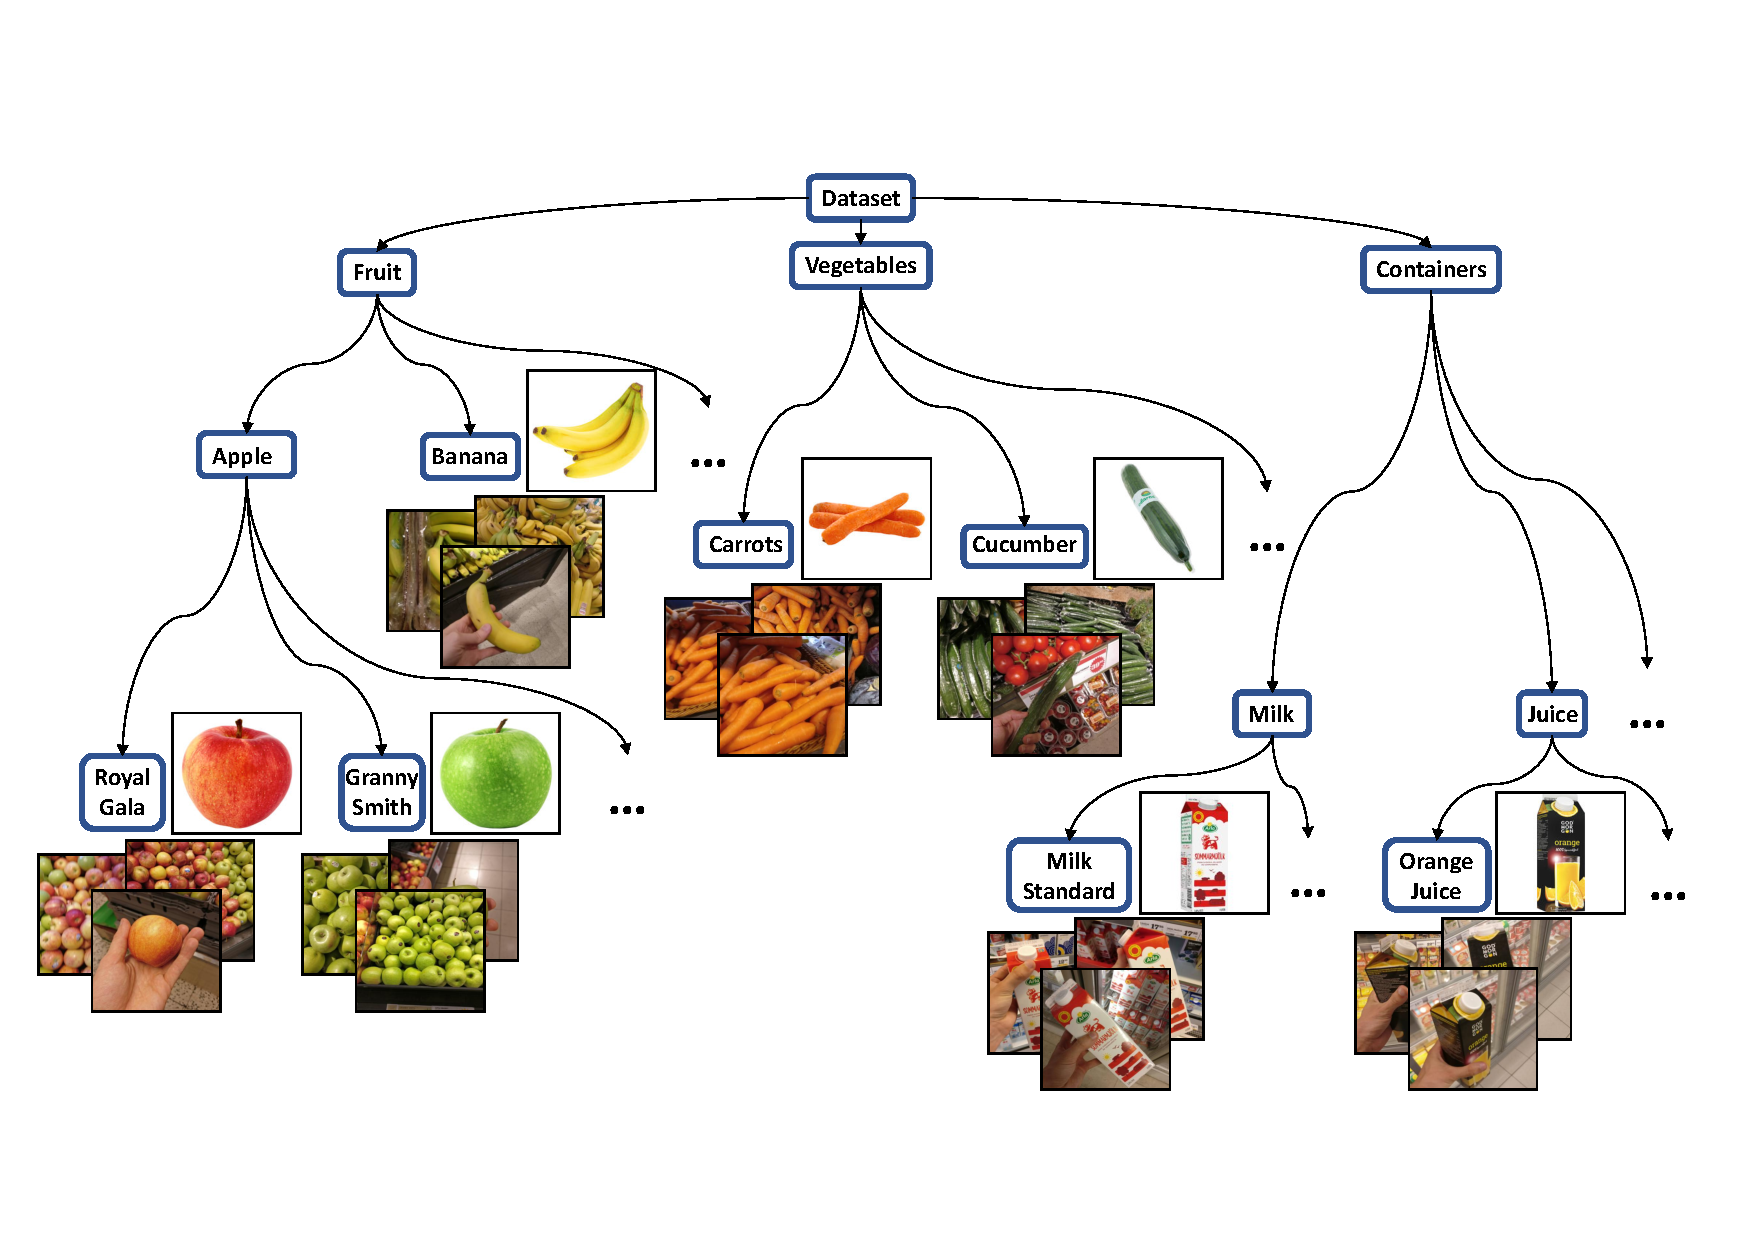
\includegraphics[width=0.9\textwidth]{PaperA/figures/intro.pdf}
    \vspace{-2mm}
    \caption{The primary contribution of this paper is a dataset of grocery items, for the purpose of training a visual recognition system to aid visually impaired people. The dataset is organized according to a hierarchical class structure, as illustrated above. A novel aspect of the dataset is that each class, apart from the semantic label, also has a visual label in the form of an iconic image.}
    \label{fig:examples} 
    \vspace{-3mm}
\end{figure}

We here address a complementary scenario not handled by current systems on the market: visual support when shopping for grocery items considering a large range of eatable objects, including fruits, vegetables, milk, and juices. 
In the case of fruits and vegetables, these are usually stacked in large bins in grocery stores as shown in Figure \ref{fig:dataset-figure}(a-f). A common problem in grocery stores is that similar items are often stacked next to each other; therefore, items are often misplaced into neighboring bins. Figure \ref{subfig:real-image-a} shows a mix of red and green apples, where it might be difficult for the system to determine which kind of apple is the actual target.
Humans can distinguish between groceries without vision to some degree, e.g.~by touching and smelling them, but it requires prior knowledge about texture and fragrance of food items.

Moreover, in addition to raw grocery items, there are also items that can only be differentiated with the help of visual information, e.g. milk, juice, and yogurt cartons, see Figure \ref{fig:dataset-figure}(g-i). Such items usually have barcodes, that are readable using the existing assistive devices described above. However, the barcodes are not easily located by visually impaired persons. Thus, an assistive vision device that fully relies on natural image understanding would be of significant added value for a visually impaired person shopping in a grocery store.

Image recognition models used for this task typically require training images collected in similar environments. However, current benchmark datasets, such as ImageNet \citeA{paperA:deng2009imagenet} and CIFAR-100 \citeA{paperA:Krizhevsky2009cifar100}, do contain images of fruits and vegetables, but are not suitable for this type of assistive application, 
since the target objects are commonly not presented in this type of natural environments, with occlusion and cluttered backgrounds. To address this issue, we present a novel dataset containing natural images of various raw grocery items and refrigerated products, e.g. milk, juice, and yogurt, taken in grocery stores. As part of our dataset, we collect images taken with single and multiple target objects, from various perspectives, and with noisy backgrounds.

In computer vision, previous studies have shown that model performance can be improved by extending the model to utilize other data sources, e.g. text, audio, in various machine learning tasks \citeA{paperA:frome2013DeVISE, paperA:Gebru2017FineGrainedCD, paperA:karpathy2015deepvisualsemantic, paperA:ngiam2011multimodal}. Descriptions of images are rather common to computer vision datasets, e.g. Flickr30k \citeA{paperA:plummer2015flickr30k}, whereas the datasets in \citeA{paperA:Gebru2017FineGrainedCD, paperA:Lin2014MicrosoftCoco} includes both descriptions and a reference image with clean background to some objects. Therefore, in addition to the natural images, we have collected iconic images with a single object centered in the image (see Figure \ref{fig:clean-image-figure}) and a corresponding product description to each grocery item. In this work, we also demonstrate how we can benefit from using additional information about the natural images by applying the multi-view generative model.

To summarize, the contribution of this paper is a dataset of natural images of raw and refrigerated grocery items, which could be used for evaluating and training image recognition systems to assist visually impaired people in a grocery store. 
The dataset labels have a hierarchical structure with both coarse- and fine-grained classes (see Figure \ref{fig:examples}). Moreover, 
each class also has an iconic image and a product description, which makes the dataset applicable to multimodal learning models. The dataset is described in Section \ref{sec:our-dataset}. 

We provide multiple benchmark results using various deep neural networks, such as Alexnet \citeA{paperA:krizhevsky2012imagenet}, VGG \citeA{paperA:simonyan2014verydeep}, DenseNet \citeA{paperA:huang2017densely}, as well as deep generative models, such as VAE \citeA{paperA:kingma2014autoencoding}. 
Furthermore, we adapt a multi-view VAE model to make use of the iconic images for each class (Section \ref{sec:classification-methods}), and show that it improves the classification accuracy given the same model setting (Section \ref{sec:experimental-results}). Last, we discuss possible future directions for fully using the additional information provided with the dataset and adopt more advanced machine learning methods, such as visual-semantic embeddings, to learn efficient representations of the images. 
\begin{comment}


\begin{figure*}[t] 
\centering
\begin{minipage}[t]{0.47\textwidth}
\centering
\subfigure[Royal Gala]{\label{subfig:real-image-a}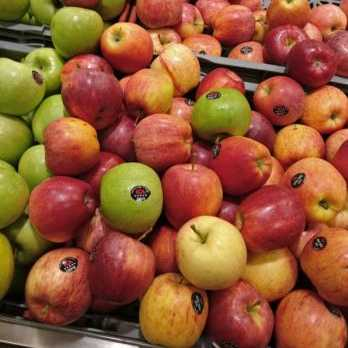
\includegraphics[width=0.30\columnwidth]{PaperA/dataset-figure/Royal-Gala-Apple_84_crop.jpg}}~
\subfigure[Golden Delicious]{\label{subfig:real-image-c}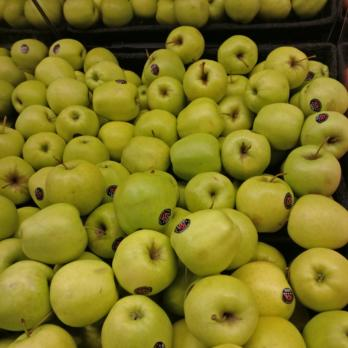
\includegraphics[width=0.30\columnwidth]{PaperA/dataset-figure/Golden-Delicious-Apple_7.jpg}}~
\subfigure[Orange]{\label{subfig:real-image-f}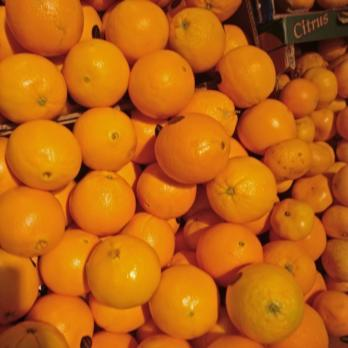
\includegraphics[width=0.30\columnwidth]{PaperA/dataset-figure/Orange_025.jpg}}~ \\ %\vspace{0.2cm}
\subfigure[Aubergine]{\label{subfig:real-image-h}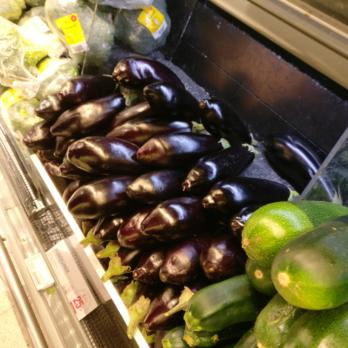
\includegraphics[width=0.30\columnwidth]{PaperA/dataset-figure/Aubergine_016.jpg}}~
\subfigure[Onion]{\label{subfig:real-image-j}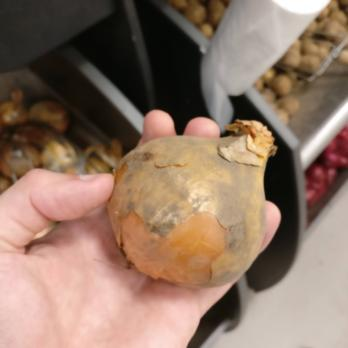
\includegraphics[width=0.30\columnwidth]{PaperA/dataset-figure/Yellow-Onion_25.jpg}}~
\subfigure[Zucchini]{\label{subfig:real-image-l}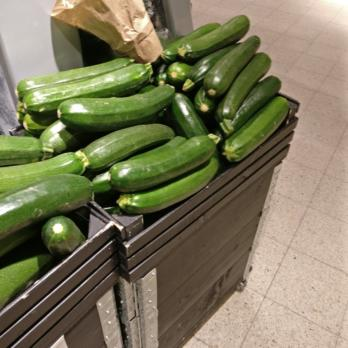
\includegraphics[width=0.30\columnwidth]{PaperA/dataset-figure/Zucchini_015.jpg}}~ \\ %\vspace{0.2cm}
\subfigure[Apple Juice]{\label{subfig:real-image-n}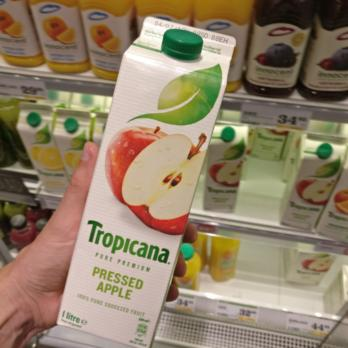
\includegraphics[width=0.30\columnwidth]{PaperA/dataset-figure/Tropicana-Apple-Juice_16.jpg}}~
\subfigure[Milk Medium Fat]{\label{subfig:real-image-q}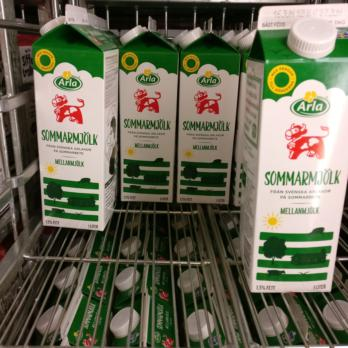
\includegraphics[width=0.30\columnwidth]{PaperA/dataset-figure/Arla-Milk-Medium-Fat_17.jpg}}~
\subfigure[Yogurt Natural]{\label{subfig:real-image-r}
\includegraphics[width=0.30\columnwidth]{PaperA/dataset-figure/Arla-Natural-Yoghurt_031.jpg}}~
   \caption{Examples of natural images in our dataset, where each image have been taken inside a grocery store. Image examples of fruits, vegetables and refrigerated products are presented in each row respectively.
   }
\label{fig:PaperA/dataset-figure}
\end{minipage}
\hspace{10pt}
\begin{minipage}[t]{0.47\textwidth}
\vspace{0pt}
\centering
\subfigure[Royal Gala]{\label{subfig:clean-img-a}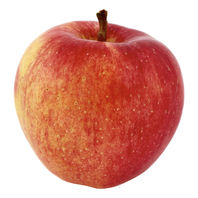
\includegraphics[width=0.30\columnwidth]{PaperA/clean-image-figure/Royal-Gala-Apple_Clean.jpg}}~
\subfigure[Golden Delicious]{\label{subfig:clean-img-c}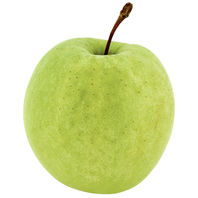
\includegraphics[width=0.30\columnwidth]{PaperA/clean-image-figure/Golden-Delicious-Apple_Clean.jpg}}~
\subfigure[Orange]{\label{subfig:clean-img-f}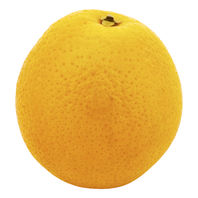
\includegraphics[width=0.30\columnwidth]{PaperA/clean-image-figure/Orange_Clean.jpg}}~ \\ %\vspace{-0.2cm}
\subfigure[Aubergine]{\label{subfig:clean-img-h}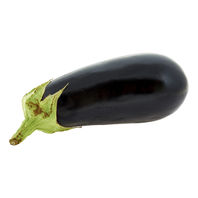
\includegraphics[width=0.30\columnwidth]{PaperA/clean-image-figure/Aubergine_Clean.jpg}}~
\subfigure[Onion]{\label{subfig:clean-img-j}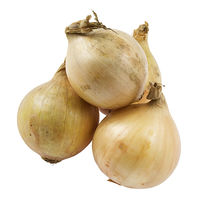
\includegraphics[width=0.30\columnwidth]{PaperA/clean-image-figure/Yellow-Onion_Clean.jpg}}~
\subfigure[Zucchini]{\label{subfig:clean-img-l}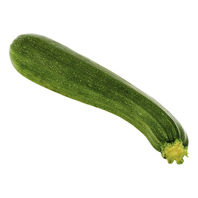
\includegraphics[width=0.30\columnwidth]{PaperA/clean-image-figure/Zucchini_Clean.jpg}}~ \\ %\vspace{-0.2cm}
\subfigure[Apple Juice]{\label{subfig:clean-img-n}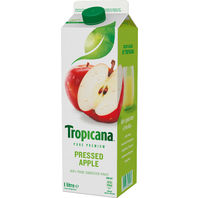
\includegraphics[width=0.30\columnwidth]{PaperA/clean-image-figure/Tropicana-Apple-Juice_Clean.jpg}}~
\subfigure[Milk Medium Fat]{\label{subfig:clean-img-q}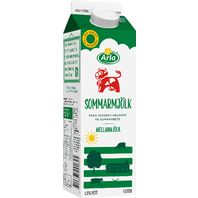
\includegraphics[width=0.30\columnwidth]{PaperA/clean-image-figure/Arla-Milk-Medium-Fat_Clean.jpg}}~
\subfigure[Yogurt Natural]{\label{subfig:clean-img-r}
\includegraphics[width=0.30\columnwidth]{PaperA/clean-image-figure/Arla-Natural-Yoghurt_Clean.jpg}}~
   \caption{Examples of iconic images downloaded from a grocery shopping website, which corresponds to the target items in the images in Figure \ref{fig:PaperA/dataset-figure}.}
\label{fig:PaperA/clean-image-figure}
\end{minipage}
\end{figure*}
\end{comment}

\section{Related Work}\label{paperA:sec:related-work}

Many popular image datasets have been collected by downloading images from the web \citeA{paperA:deng2009imagenet, paperA:Everingham2010pascal, paperA:Gebru2017FineGrainedCD,  paperA:griffin2007caltech256, paperA:Krizhevsky2009cifar100, paperA:Lin2014MicrosoftCoco, paperA:song2016deep, paperA:welinder2010birds, paperA:xiao2010sundatabase}. 
If the dataset contains a large amount of images, it is convenient to make use of crowdsourcing to get annotations for recognition tasks \citeA{paperA:deng2009imagenet, paperA:Krizhevsky2009cifar100, paperA:liu2015faceattributes}. For some datasets, the crowdsourcers are also asked to put bounding boxes around the object to be labeled for object detection tasks \citeA{paperA:Everingham2010pascal, paperA:Gebru2017FineGrainedCD, paperA:welinder2010birds}. In \citeA{paperA:griffin2007caltech256} and \citeA{paperA:Krizhevsky2009cifar100}, the target objects are usually centered and takes up most content of the image itself. Another significant characteristic is that web images usually are biased in the sense that they have been taken with the object focus in mind; they have good lighting settings and are typically clean from occlusions, since the collectors have used general search words for the object classes, e.g. \textit{car}, \textit{horse}, or \textit{apple}.

Some datasets include additional information about the images beyond the single class label, e.g. text descriptions of what is present in the image and bounding boxes around objects. These datasets can be used in several different computer vision tasks, such as image classification, object detection, and image segmentation. Structured labeling is another important property of a dataset, which provides flexibility when classifying images. In  \citeA{paperA:Gebru2017FineGrainedCD, paperA:Lin2014MicrosoftCoco}, all of these features exist and moreover they include reference images to each object class, which in \citeA{paperA:Lin2014MicrosoftCoco} is used for labeling multiple  categories present in images, while in \citeA{paperA:Gebru2017FineGrainedCD} these images are used for fine-grained recognition. 
Our dataset includes a reference image, i.e. the iconic image, and a product description for every class, and we have also labeled the grocery items in a structured manner.

Other image datasets of fruits and vegetables for classification purposes are the FIDS30 database \citeA{paperA:marko2013fids30} and the dataset in \citeA{paperA:muresan2017fruit}. The images in FIDS30 were downloaded from the web and contain background noise as well as single or multiple instances of the object. In \citeA{paperA:muresan2017fruit}, all pixels belonging to the object are extracted from the original image, such that all images have white backgrounds with the same brightness condition. There also exist datasets for detecting fruits in orchards for robotic harvesting purposes, which are very challenging since the images contain plenty of background and various lighting conditions, and the targeted fruits are often occluded or of the same color as the background \citeA{paperA:bargoti2017deepfruitdetection, paperA:sa2016deepfruits}.

Another dataset that is highly relevant to our application need is presented in  \citeA{paperA:waltner2015mango}. They collected a dataset for training and evaluating the image classifier by extracting images from video recordings of 23 main classes, which are subdivided into 98 classes, of raw grocery items (fruits and vegetables) in different grocery stores. Using this dataset, a mobile application was developed to recognize food products in grocery store environments, which provides the user with details and health recommendations about the item along with other proposals of similar food items. For each class, there exists a product description with nutrition values to assist the user in shopping scenarios. The main difference between this work and our dataset is firstly the clean iconic images (visual labels) for each class in our dataset, and secondly that we have also collected images of refrigerated items, such as dairy and juice containers, where visual information is required to distinguish between the products.   

\section{Our Dataset}\label{paperA:sec:our-dataset}

We have collected images from fruit and vegetable sections and refrigerated sections with dairy and juice products in 18 different grocery stores. The dataset consists of 5125 images from 81 fine-grained classes, where the number of images in each class range from 30 to 138. Figure \ref{fig:hist} displays a histogram over the number of images per class. As illustrated in Figure \ref{fig:examples}, the class structure is hierarchical, and there are 46 coarse-grained classes. Figure \ref{fig:dataset-figure} shows examples of the collected natural images. For each fine-grained class, we have downloaded an iconic image of the item and also a product description including origin country, an appreciated weight and nutrient values of the item from a grocery store website. Some examples of downloaded iconic images can be seen in Figure \ref{fig:clean-image-figure}. 

Our aim has been to collect the natural images under the same condition as they would be as part of an assistive application on a mobile phone. All images have been taken with a 16-megapixel Android smartphone camera from different distances and angles. Occasionally, the images include other items in the background or even items that have been misplaced in the wrong shelf along with the targeted item. It is important that image classifiers that are used for assisting devices are capable of performing well with such noise since these are typical settings in a grocery store environments. The lighting conditions in the images can also vary depending on where the items are located in the store. 
Sometimes the images are taken while the photographer is holding the item in the hand. This is often the case for refrigerated products since these containers are usually stacked compactly in the refrigerators. For these images, we have consciously varied the position of the object, such that the item is not always centered in the image or present in its entirety. 

We also split the data into a training set and test set based on the application need. Since the images have been taken in several different stores at specific days and time stamps, 
parts of the data will have similar lighting conditions and backgrounds for each photo occasion. To remove any such biasing correlations, all images of a certain class taken at a certain store are assigned to either the test set or training set. Moreover, we balance the class sizes to as large extent as possible in both the training and test set. After the partitioning, the training and test set contains 2640 and 2485 images respectively. Predefining a training and test set also makes it easier for other users to compare their results to the evaluations in this paper.

The task is to classify natural images using mobile devices to aid visually impaired people. The additional information such as the hierarchical structure of the class labels, iconic images, and product descriptions can be used to improve the performance of the computer vision system. Every class label is associated with a product description. Thus, the product description itself can be part of the output for visually impaired persons as they may not be able to read what is printed on a carton box or a label tag on a fruit bin in the store.

%Collecting and labeling real-world data is a time-costly procedure. 
%Therefore, we propose that the natural images can be combined with additional information of the target object in the form of text and iconic images.
The dataset is intended for research purposes and we are open to contributions with more images and new suitable classes. Our dataset is available at \url{https://github.com/marcusklasson/GroceryStoreDataset}. Detailed instructions on how to contribute to the dataset can be found on our dataset webpage.



\begin{figure}[t]
\centering
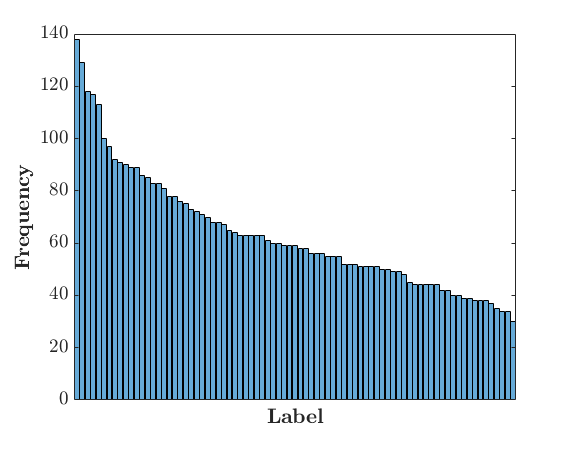
\includegraphics[width=\columnwidth,height=0.20\paperheight]{PaperA/figures/hist1_latex_bf14.png}
\caption{Histogram over the number of images in each class in the dataset.}
\label{fig:hist}
\end{figure}


\section{Classification Methods}\label{paperA:sec:classification-methods}

We here describe the classification methods and approaches that we have used to provide benchmark results to the dataset. We apply both deterministic deep neural networks as well as a deep generative model used for representation learning to the natural images that we have collected. Furthermore, we utilize the additional information -- iconic images -- from our dataset with a multi-view deep generative model. This model can utilize different data sources and obtain superior representation quality as well as high interpretability. For a fair evaluation, we use a linear classifier with the learned representation from the different methods.

\paragraph*{Deep Neural Networks.} 
CNNs have been the state-of-the-art models in image classification ever since AlexNet \citeA{paperA:krizhevsky2012imagenet} achieved the best classification accuracy in ILSVRC in 2012.
However, in general, computer vision models require lots of labeled data to achieve satisfactory performance, which has resulted in interest for adapting CNNs that have already been trained on a large amount of training data to other image datasets. When adapting pretrained CNNs to new datasets, we can either use it directly as a feature extractor, a.k.a use the off-the-shelf features,~\citeA{paperA:donahue2014decaf, paperA:razavian2014cnnfeatures}, or fine-tune it~\citeA{paperA:Girshick2014rich-feature-hierarchies, paperA:oquab2014learning-and-transferring, paperA:pan2010transferlearning, paperA:yosinski2014transferable, paperA:Zhang2014PartbasedRCNN}. Using off-the-shelf features, we need to specify which feature representation we should extract from the network and use these for training a new classifier. Fine-tuning a CNN involves adjusting the pretrained model parameters, such that the network can e.g. classify images from a dataset different from what the CNN was trained on before. We can either choose to fine-tune the whole network or select some layer parameters to adjust while keeping the others fixed. One important factor on deciding which approach to choose is the size of the new dataset and how similar the new dataset is to the dataset which the CNN was previously trained on. A rule of thumb here is that the closer the features are to the classification layer, the features become more specific to the training data and task \citeA{paperA:yosinski2014transferable}. 

Using off-the-shelf CNN features and fine-tuned CNNs have been successfully applied in \citeA{paperA:donahue2014decaf, paperA:razavian2014cnnfeatures} and \citeA{paperA:Girshick2014rich-feature-hierarchies, paperA:oquab2014learning-and-transferring, paperA:Zhang2014PartbasedRCNN} respectively.
In \citeA{paperA:donahue2014decaf, paperA:razavian2014cnnfeatures}, it is shown that the pretrained features have sufficient representational power to generalize well to other visual recognition tasks with simple linear classifiers, such as Support Vector Machines (SVMs), without fine-tuning the parameters of the CNN to the new task. In \citeA{paperA:Girshick2014rich-feature-hierarchies, paperA:Zhang2014PartbasedRCNN}, all CNN parameters are fine-tuned, whereas in \citeA{paperA:oquab2014learning-and-transferring} the pretrained CNN layer parameters are kept fixed and only an adaptation layer of two fully connected layers are trained on the new task. The results from these works motivate why we should evaluate our dataset on fine-tuned CNNs or linear classifiers trained on off-the-shelf feature representations instead of training an image recognition model from scratch. 

\vspace{-3mm}
\paragraph{Variational Autoencoders with only natural images.}
Deep generative models, 
e.g. the variational autoencoder (VAE)~\citeA{paperA:kingma2014autoencoding, paperA:Rezende2014StochasticBA, paperA:zhang2017advances}, have become widely used in the machine learning community thanks to their generative nature. We thus use VAEs for representation learning as the second benchmarking method. For efficiency, we use low-level pretrained features from a CNN as inputs to the VAE.

The latent representations from VAEs are encodings of the underlying factors for how the data are generated. VAEs belongs to the family of latent variable models, which commonly has the form $p_{\boldsymbol{\theta}}(\mathbf{x},\mathbf{z}) = p(\mathbf{z}) p_{\boldsymbol{\theta}}(\mathbf{x}|\mathbf{z})$, where $p(\mathbf{z})$ is a prior distribution over the latent variables $\mathbf{z}$ and $p_{\boldsymbol{\theta}}(\mathbf{x}|\mathbf{z})$ is the likelihood over the data $\mathbf{x}$ given $\mathbf{z}$. The prior distribution is often assumed to be Gaussian,
$p(\mathbf{z}) = \mathcal{N}(\mathbf{z}\,|\, \boldsymbol{0}, \mathbf{I})$,  
whereas the likelihood distribution depends on the values of $\mathbf{x}$.
The likelihood $p_{\boldsymbol{\theta}}(\mathbf{x}|\mathbf{z})$ is referred to as a decoder represented as a neural network parameterized by $\boldsymbol{\theta}$. An encoder network $q_{\boldsymbol{\phi}}(\mathbf{z}|\mathbf{x})$ parameterized by $\boldsymbol{\phi}$ is introduced as an approximation of the true posterior $p_{\boldsymbol{\theta}}(\mathbf{z}|\mathbf{x})$, which is intractable since it requires computing the integral $p_{\boldsymbol{\theta}}(\mathbf{x}) = \int p_{\boldsymbol{\theta}}(\mathbf{x}, \mathbf{z}) \, d\mathbf{z}$. 
When the prior distribution is a Gaussian, the approximate posterior is also modeled as a Gaussian, $q_{\boldsymbol{\phi}}(\mathbf{z}|\mathbf{x}) = \mathcal{N}(\mathbf{z} \,|\,\boldsymbol{\mu}(\mathbf{x}), \boldsymbol{\sigma}^2(\mathbf{x}) \odot \mathbf{I})$, with some mean $\boldsymbol{\mu}(\mathbf{x})$ and variance $\boldsymbol{\sigma}^2(\mathbf{x})$ computed by the encoder network. The goal is to maximize the marginal log-likelihood by defining a lower bound using $q_{\boldsymbol{\phi}}(\mathbf{z}|\mathbf{x})$:
\begin{align}
\begin{split}\label{eq:vae-loss}
\log p_{\boldsymbol{\theta}}(\mathbf{x}) \geq \mathcal{L}(\boldsymbol{\theta}, \boldsymbol{\phi}; \mathbf{x}) = & \mathbb{E}_{q_{\boldsymbol{\phi}}(\mathbf{z}|\mathbf{x})}\left[\, \log p_{\boldsymbol{\theta}}(\mathbf{x} | \mathbf{z}) \,\right] \\ & -D_{KL}(q_{\boldsymbol{\phi}}(\mathbf{z}|\mathbf{x})\,||\,p(\mathbf{z})) .
\end{split}
\end{align}
The last term is the Kullback-Leibler (KL) divergence of the approximate posterior from the true posterior. The lower bound $\mathcal{L}$ is called the evidence lower bound (ELBO) and can be optimized with stochastic gradient descent via backpropagation \citeA{paperA:doersch2016tutorialvae, paperA:kingma2014autoencoding}. 
VAE is a probabilistic framework. Many extensions such as utilizing structured priors\citeA{paperA:butepage2018Inform} or using continual learning \citeA{paperA:nguyen2018variational} have been explored.
%In fully supervised learning settings, we would have to retrain the model when a new class is introduced. 
%Another advantage is that VAEs can be extended to multimodal data and learn joint latent representations between data pairs, such as image--text or image--image. 
In the following method, we describe how to make use of the iconic images while retaining the unsupervised learning setting in VAEs.

\vspace{-3mm}
\paragraph{Utilizing iconic images with multi-view VAEs.}
Utilizing extra information has shown to be useful in many applications with various model designs~\citeA{paperA:butepage2018Inform, paperA:vedantam2018generative, paperA:vinyals2015show, paperA:wang2016vcca, paperA:zhang2016inter}. For computer vision tasks, natural language is the most commonly used modality to aid the visual representation learning. However, the consistency of the language and visual embeddings has no guarantee. As an example with our dataset, the product description of a Royal Gala apple explains the appearance of a red apple. But if the description is represented with word embeddings, e.g. word2vec \citeA{paperA:mikolov2013distributedrepresentations}, the word 'royal' will probably be more similar to the words 'king' and 'queen' than 'apple'. Therefore, if available, additional visual information about objects might be more beneficial for learning meaningful representations instead of text. In this work, with our collected dataset, we propose to utilize the iconic images for the representation learning of natural images using a multi-view VAE. Since the natural images can include background noise and grocery items different from the targeted one, the role of the iconic image will be to guide the model to which features that are of interest in the natural image.

The VAE can be extended to modeling multiple views of data, where a latent variable $\mathbf{z}$ is assumed to have generated the views \citeA{paperA:vedantam2018generative, paperA:wang2016vcca}. Considering two views $\mathbf{x}$ and $\mathbf{y}$, the joint distribution over the paired random variables ($\mathbf{x}$, $\mathbf{y}$) and latent variable $\mathbf{z}$ can be written as $p_{\boldsymbol{\theta}}(\mathbf{x}, \mathbf{y}, \mathbf{z}) = p(\mathbf{z})p_{\boldsymbol{\theta^{(1)}}}(\mathbf{x}\,|\,\mathbf{z})p_{\boldsymbol{\theta^{(2)}}}(\mathbf{y}\,|\,\mathbf{z})$, where both $p_{\boldsymbol{\theta^{(1)}}}(\mathbf{x}\,|\,\mathbf{z})$ and $p_{\boldsymbol{\theta^{(2)}}}(\mathbf{y}\,|\,\mathbf{z})$ are represented as neural networks with parameters $\boldsymbol{\theta^{(1)}}$ and $\boldsymbol{\theta^{(2)}}$. Assuming that the latent variable $\mathbf{z}$ can reconstruct both $\mathbf{x}$ and $\mathbf{y}$ when only $\mathbf{x}$ is encoded into $\mathbf{z}$ by the encoder $q_{\boldsymbol{\phi}}(\mathbf{z}|\mathbf{x})$, then the ELBO is written as 
\begin{align}
\begin{split}\label{eq:vcca-loss}
\log p_{\boldsymbol{\theta}}(\mathbf{x}, \mathbf{y}) \geq & \, \mathcal{L}(\boldsymbol{\theta}, \boldsymbol{\phi}; \mathbf{x}, \mathbf{y}) \\ 
= & \,  \mathbb{E}_{q_{\boldsymbol{\phi}}(\mathbf{z}|\mathbf{x})}\left[\, \log p_{\boldsymbol{\theta^{(1)}}}(\mathbf{x} | \mathbf{z}) + \log p_{\boldsymbol{\theta^{(2)}}}(\mathbf{y} | \mathbf{z}) \,\right] \\ 
& -D_{KL}(q_{\boldsymbol{\phi}}(\mathbf{z}|\mathbf{x})\,||\,p(\mathbf{z})) .
\end{split}
\end{align}  
This model is referred to as variational autoencoder canonical correlation analysis (VAE-CCA) and was introduced in \citeA{paperA:wang2016vcca}. The main motivation for using VAE-CCA is that the latent representations need to contain information about reconstructing both natural and iconic images.
The main motivation for using VAE-CCA is that 
the latent representation needs to preserve information about how both the natural and iconic images are reconstructed. This also allows us to produce iconic images from new natural images to enhance the interpretability of the latent representation of VAE-CCA (see Section \ref{paperA:sec:experimental-results}) \citeA{paperA:vedantam2018generative}.

%\begin{comment}
	
\begin{figure}[t]
    \centering
    \begin{subfigure}[b]{0.35\textwidth}
    	\centering
    	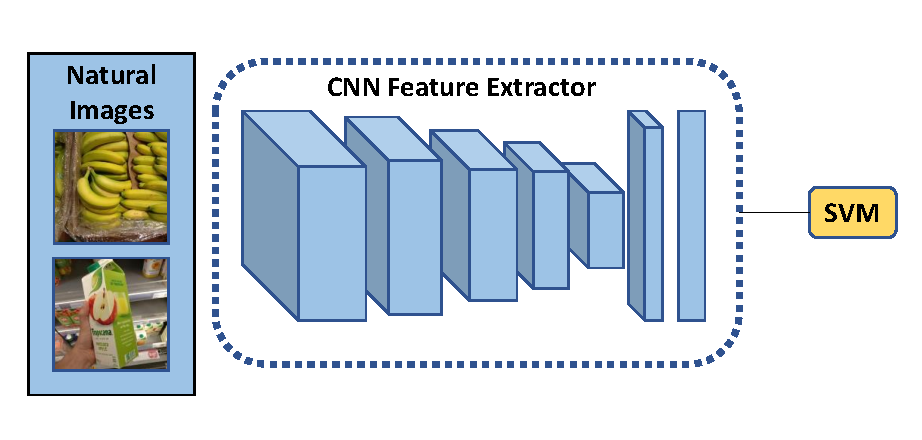
\includegraphics[width=\textwidth]{PaperA/figures/cnn.pdf}
    	%\vspace{-7mm}
    	\caption{}
    	\label{subfig:cnn}
    \end{subfigure} ~
    \begin{subfigure}[b]{0.6\textwidth}
		\centering
		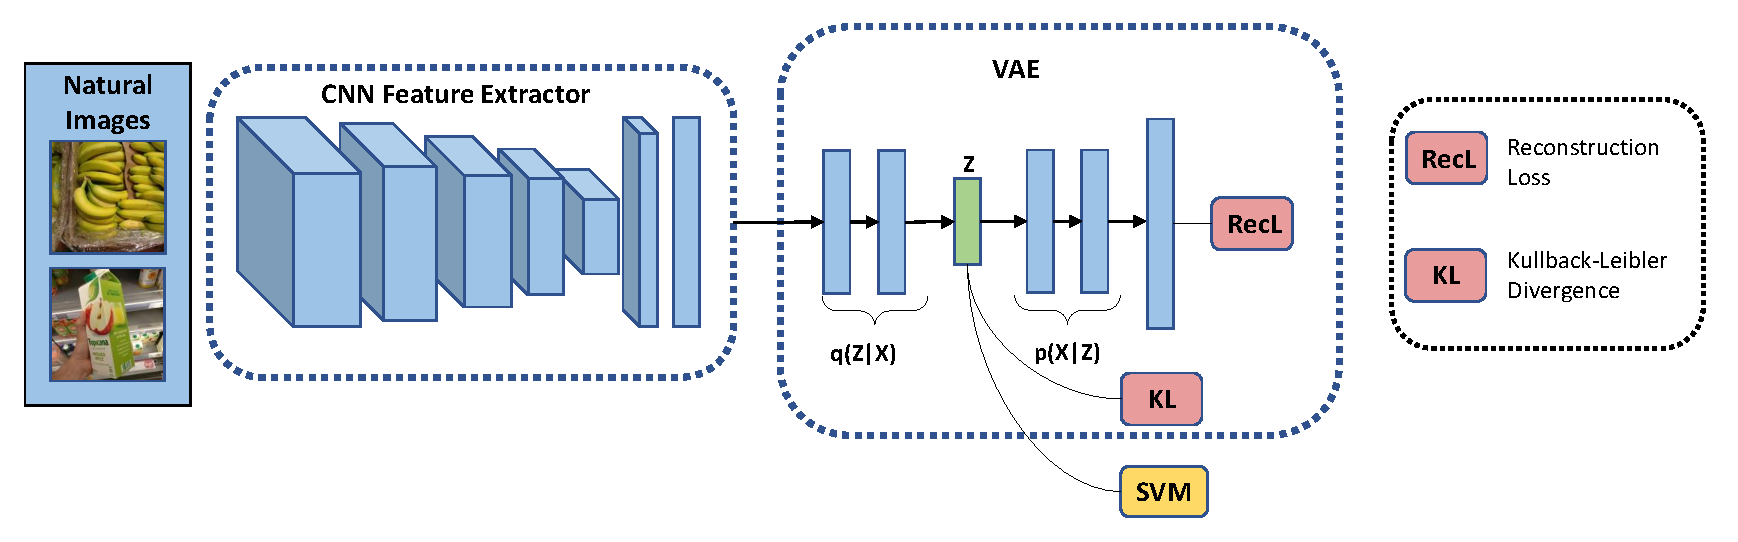
\includegraphics[width=\textwidth]{PaperA/figures/cnn+vae.pdf}
		%\vspace{-7mm}
		\caption{}
		\label{subfig:cnn+vae}
	\end{subfigure} \\
    \begin{subfigure}[b]{0.7\textwidth}
		\centering
		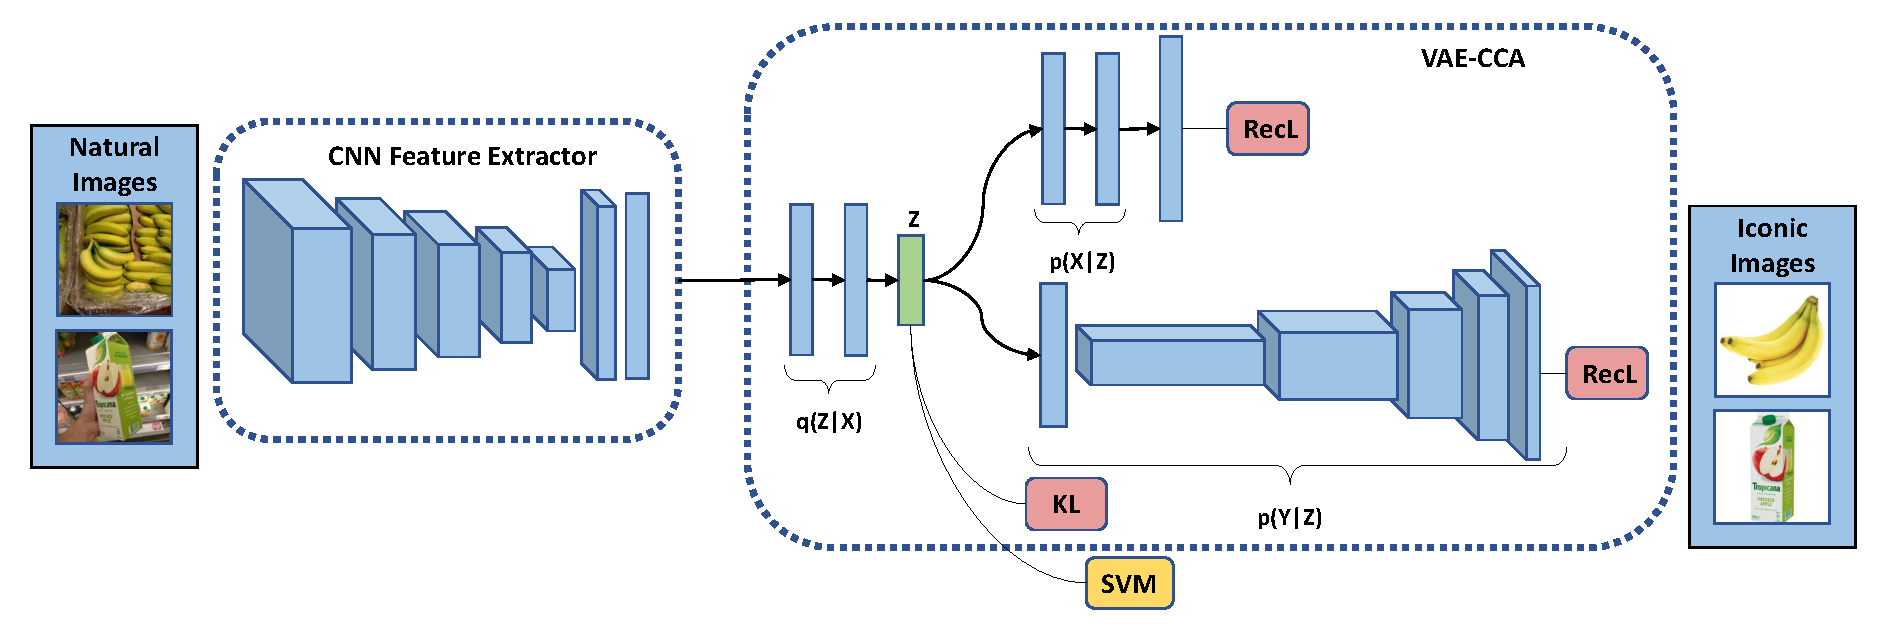
\includegraphics[width=\textwidth]{PaperA/figures/vae-cca.pdf}
		%\vspace{-7mm}
		\caption{}
		\label{subfig:vae-cca}
	\end{subfigure}
    %\subfigure[CNN]{\label{subfig:cnn}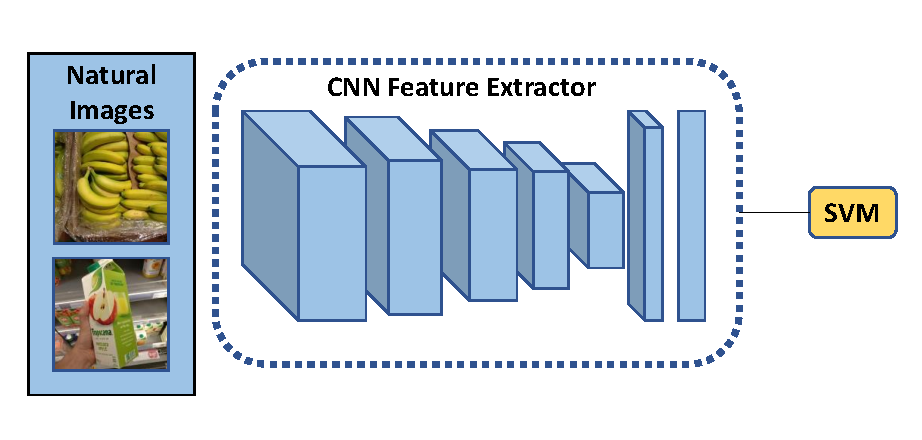
\includegraphics[width=0.35\textwidth]{PaperA/figures/cnn.pdf}} 
    %\subfigure[VAE]{\label{subfig:cnn+vae}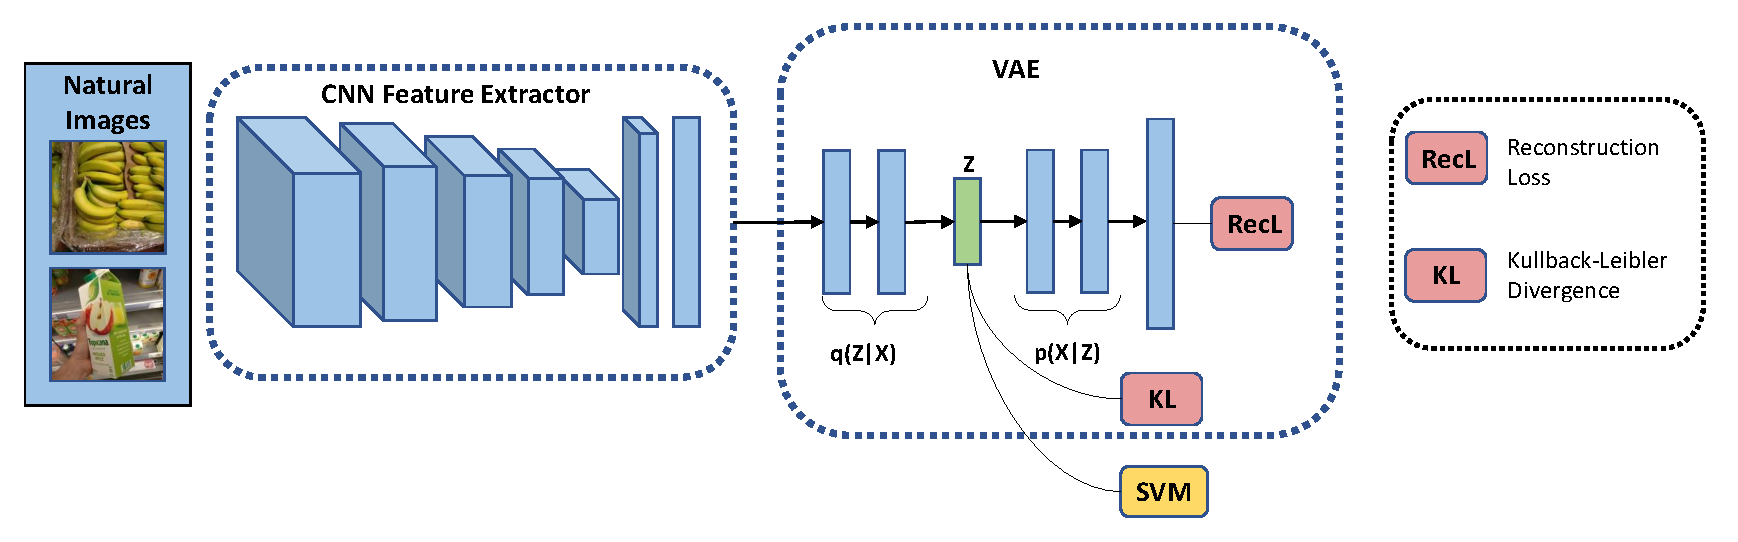
\includegraphics[width=0.6\textwidth]{PaperA/figures/cnn+vae.pdf}}
    %\subfigure[VAE-CCA]{\label{subfig:vae-cca}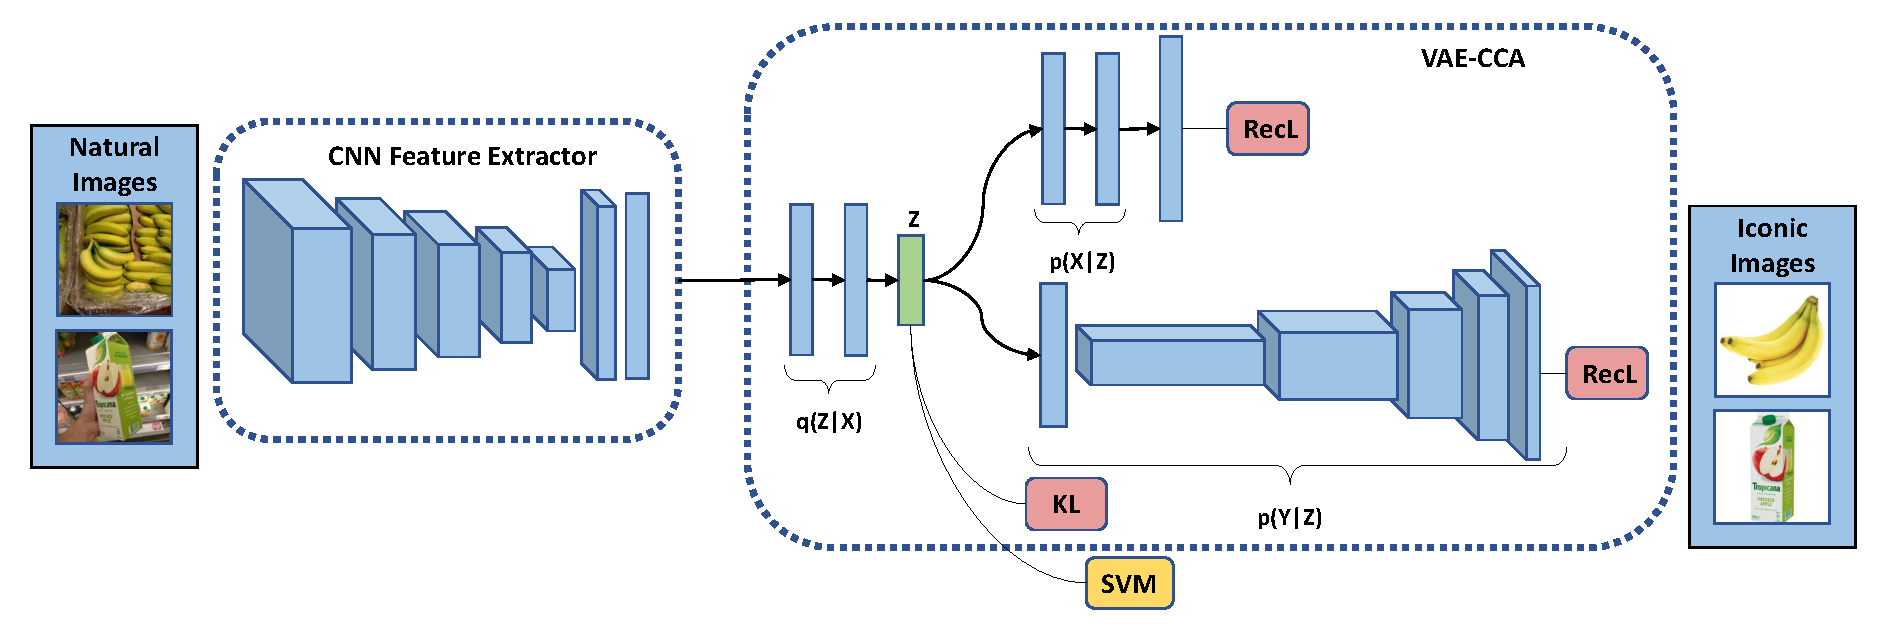
\includegraphics[width=0.7\textwidth]{PaperA/figures/vae-cca.pdf}}
    \caption{The architectures for the classification methods described in Section \ref{paperA:sec:classification-methods}. In this paper, we use either a pretrained AlexNet, VGG16 or DenseNet-169 as the CNN feature extractor, but it may be replaced with any CNN architecture. Note that the pretrained CNN can be fine-tuned. The encoder and decoder of the VAE in \ref{subfig:cnn+vae} consist of two fully-connected layers. VAE-CCA in \ref{subfig:vae-cca} uses the DCGAN architecture as an iconic image decoder and the same encoder and feature vector decoder as the VAE.   }
    \label{fig:classification-methods}
\end{figure}

%\end{comment}
\section{Experimental Results}\label{paperA:sec:experimental-results}

We apply the three different types of models described in Section \ref{sec:classification-methods} to our dataset and evaluate their performance. The natural images are propagated through a CNN pretrained on ImageNet to extract feature vectors. We experiment with both the off-the-shelf features as well as fine-tuning the CNN. When using off-the-shelf features, we simply extract feature vectors and train an SVM on those. For the fine-tuned CNN, we report both results from the softmax classifier used in the actual fine-tuning procedure and training an SVM with extracted fine-tuned feature vectors.  

These extracted feature vectors are also used for VAE and VAE-CCA which makes further compression. We perform classification for those VAE based models by training a classifier, e.g. an SVM, on the data encoded into the latent representation. We use this classification approach for both VAE and VAE-CCA. In all classification experiments, except when we fine-tune the CNN, we use a linear SVM trained with the one-vs-one approach as in \citeA{paperA:razavian2014cnnfeatures}.

We experiment with three different pretrained CNN architectures, namely AlexNet \citeA{paperA:krizhevsky2012imagenet}, VGG16 \citeA{paperA:simonyan2014verydeep} and DenseNet-169 \citeA{paperA:huang2017densely}. For AlexNet and VGG16, we extract feature vectors of size 4096 from the two last fully connected (FC) layers before the classification layer. The features from the $n^{\text{th}}$ hidden layer are denoted as $\text{AlexNet}_{n}$ and $\text{VGG16}_{n}$. As an example, the last hidden FC layer in AlexNet is denoted as $\text{AlexNet}_{7}$, the input of which is output from $\text{AlexNet}_{6}$. For DenseNet-169, we extract the features of size 1664 from the average pooling layer before its classification layer.

%\renewcommand{\arraystretch}{1.2}
\begin{table}[t]
    \centering
    \caption{ Fine-grained classification (81 classes) accuracies with the methods described in Section \ref{subsec:experimental-setups}. Each row displays from which network architecture and layer that we extracted the feature vectors of the natural images. The columns show the result from the classifiers that we used (see Section \ref{subsec:experimental-setups}). }
    \vspace{-3mm}
    \resizebox{\textwidth}{!}{%
    \begin{tabular}{c c c c c c c}
        \hline
        %\Xhline{3\arrayrulewidth}
        & SVM & SVM-ft & VAE+SVM & VAE+SVM-ft & VAE-CCA+SVM & VAE-CCA+SVM-ft  \\
        \hline
        %\Xhline{3\arrayrulewidth}
        \rowcolor{gray!25}
         $\text{AlexNet}_{6}$  &  69.2 & 72.6 & 65.6 & 70.7 & 67.8	& 71.5 \\
         $\text{AlexNet}_{7}$ &  65.0 & 70.7 & 63.0 & 68.7 & 65.0 & 70.9 \\
         %\hline
        \rowcolor{gray!25}
         $\text{VGG16}_{6}$ &  62.1	& 73.3 & 57.5 & 71.9 & 60.7 & 73.0 \\
         $\text{VGG16}_{7}$ & 57.3	& 71.7 & 56.8 & 67.8 & 56.8 & 71.3 \\
         %\hline
        \rowcolor{gray!25}
         $\text{DenseNet-169}$ & 72.5 & 85.0 & 65.4 & 79.1 & 72.6 & 80.4 \\
        %\Xhline{3\arrayrulewidth}
        \hline
    \end{tabular} }
    \label{tab:results-fine-grained}
\end{table}

%\renewcommand{\arraystretch}{1.2}
\begin{table}[t]
    \centering
    \caption{Coarse-grained classification (46 classes) accuracies with an SVM for the methods described in Section \ref{subsec:experimental-setups} that uses off-the-shelf feature representations. Each row displays from network architecture and layer that we extracted the feature vectors of the natural images and the columns show the result for the classification methods. }
    \vspace{2mm}
    \scalebox{0.95}{
    \begin{tabular}{c ccc}
        \hline %\Xhline{3\arrayrulewidth}
         & SVM & VAE+SVM & VAE-CCA+SVM  \\
        \hline %\Xhline{3\arrayrulewidth}
        \rowcolor{gray!25}
         $\text{AlexNet}_{6}$ & 78.0 & 74.2 & 76.4  \\ 
         $\text{AlexNet}_{7}$ & 75.4 & 73.2 & 74.4  \\ 
        \rowcolor{gray!25}
         $\text{VGG16}_{6}$ &  76.6 & 74.2 & 74.9  \\ 
         $\text{VGG16}_{7}$ & 72.8 & 71.7 & 72.3  \\
         \rowcolor{gray!25}
         $\text{DenseNet-169}$ & 85.2 & 79.5 & 82.0 \\
        \hline %\Xhline{3\arrayrulewidth}
    \end{tabular}
    }
    \label{tab:results-coarse-grained}
\end{table}

%\renewcommand{\arraystretch}{1.25}
\begin{table}[t]
\centering
\caption{Fine-grained classification accuracies from fine-tuned CNNs pretrained on ImageNet, where the column shows which architecture that has been fine-tuned. A standard softmax layer is used as the last classification layer.
}
\vspace{2mm}
\scalebox{0.95}{
\begin{tabular}{cccc}
    \hline
    \Xhline{3\arrayrulewidth}
    & AlexNet & VGG16 & DenseNet-169 \\
    \Xhline{3\arrayrulewidth}
    \rowcolor{gray!25}
    Fine-tune &  69.3 & 73.8 & 84.0  \\
    \Xhline{3\arrayrulewidth}
\end{tabular}
}
\label{tab:results-finetuned-cnn}
\end{table}


\subsection{Experimental Setups}\label{subsec:experimental-setups}

The following setups were used in the experiments: 


\paragraph*{Setup 1.} Train an SVM on extracted off-the-shelf features from a pretrained CNN, which is denoted as SVM in the results. We also fine-tune the CNN by replacing the final layer with a new softmax layer and denote these results as Fine-tune. We denote training an SVM on extracted finetuned feature vectors as SVM-ft.


\paragraph*{Setup 2.} Extract feature vectors with a pretrained CNN of the natural images and learn a latent representation $\mathbf{z}$ with a VAE. Then the data is encoded into the latent space and we train an SVM with these latent representations, which used for classification. We denote the results as VAE+SVM when using off-the-shelf feature vectors, whereas using the fine-tuned feature vectors are denoted as VAE+SVM-ft. In all experiments with the VAE, we used the architecture from \citeA{paperA:sohn2015conditionalvae}, i.e. the latent layer having 200 hidden units and both encoder and decoder consisting of two FC layers with 1,000 hidden units each.

\paragraph*{Setup 3.} Each natural image is paired with its corresponding iconic image. We train VAE-CCA similarly as the VAE, but instead, we learn a joint latent representation that is used to reconstruct the extracted feature vectors $\mathbf{x}$ and the iconic images $\mathbf{y}$. The classification is performed with the same steps as in Setup 2 and denotes the results similarly with VAE-CCA+SVM and VAE-CCA+SVM-ft. Our VAE-CCA model takes the feature vectors $\mathbf{x}$ as input and encodes them into a latent layer with 200 hidden units. The encoder and the feature vector decoder uses the same architecture, i.e. two FC layers with 512 hidden units, whereas the iconic image decoder uses the DCGAN \citeA{paperA:radford2015unsupervised} architecture.

Figure \ref{fig:classification-methods} displays the three experimental setups described above. We report both fine-grained and coarse-grained classification results with an SVM in Table \ref{tab:results-fine-grained} and \ref{tab:results-coarse-grained} respectively. In Table \ref{tab:results-finetuned-cnn}, we report the fine-grained classification results from fine-tuned CNNs.

When fine-tuning the CNNs,
we replace the final layer with a softmax layer applicable to our dataset with randomly initialized weights drawn from a Gaussian with zero mean and standard deviation $0.01$~\citeA{paperA:Zhang2014PartbasedRCNN}. 
For AlexNet and VGG16, we fine-tune the networks for 30 epochs with two different learning rates, 0.01 for the new classification layer and 0.001 for the pretrained layers. Both learning rates are reduced by half after every fifth epoch. The DenseNet-169 is fine-tuned for 30 epochs with momentum of $0.9$ and an initial learning rate of 0.001, which decays with $10^{-6}$ after each epoch. We report the classification results from the softmax activation after the fine-tuned classification layer. 
We also report classification results from an SVM trained with feature representations from a fine-tuned CNN, which are extracted from FC6 and FC7 of the AlexNet and VGG16 and from the last average pooling layer in DenseNet-169.

The VAE and VAE-CCA models are trained for 50 epochs with Adam \citeA{paperA:kingma2015adam} for optimizing the ELBOs in Equation \ref{eq:vae-loss} and \ref{eq:vcca-loss} respectively. We use a constant learning rate of 0.0001 and set the minibatch size to 64. The extracted feature vectors are rescaled with standardization before training the VAE and VAE-CCA models to stabilize the learning.

\subsection{Results}

\begin{figure}[t]
	\centering
	\begin{subfigure}[b]{0.18\textwidth}
		\centering
		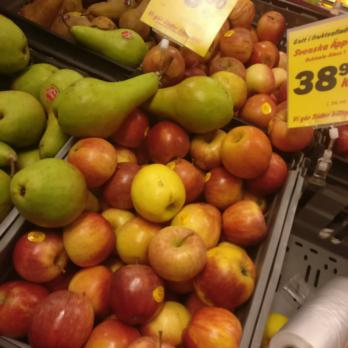
\includegraphics[width=\textwidth]{PaperA/decoded-image-figure/Royal-Gala-Apple_003.jpg}
		%\vspace{-7mm}
		\caption{}
		\label{subfig:royal-gala-natural}
	\end{subfigure} ~
	\begin{subfigure}[b]{0.18\textwidth}
		\centering
		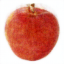
\includegraphics[width=\textwidth]{PaperA/decoded-image-figure/densenet_nov11/Royal-Gala-Apple_decoded.png}
		%\vspace{-7mm}
		\caption{}
		\label{subfig:royal-gala-decoded}
	\end{subfigure} ~~~
	\begin{subfigure}[b]{0.18\textwidth}
		\centering
		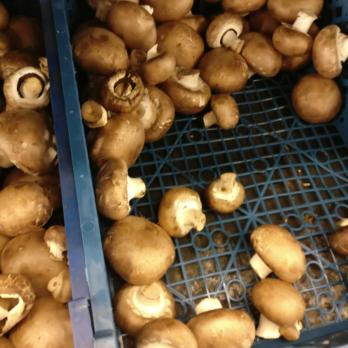
\includegraphics[width=\textwidth]{PaperA/decoded-image-figure/Mushroom-Brown-Cap_027.jpg}
		%\vspace{-7mm}
		\caption{}
		\label{subfig:brown-cap-natural}
	\end{subfigure} ~
	\begin{subfigure}[b]{0.18\textwidth}
		\centering
		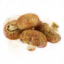
\includegraphics[width=\textwidth]{PaperA/decoded-image-figure/densenet_nov11/Mushroom-Brown-Cap_decoded.png}
		%\vspace{-7mm}
		\caption{}
		\label{subfig:brown-cap-decoded}
	\end{subfigure} \\[1mm]
	\begin{subfigure}[b]{0.18\textwidth}
		\centering
		
\includegraphics[width=\textwidth]{PaperA/decoded-image-figure/Oatly-Natural-Yoghurt_007.jpg}
		%\vspace{-7mm}
		\caption{}
		\label{subfig:oatgurt-natural}
	\end{subfigure} ~
	\begin{subfigure}[b]{0.18\textwidth}
		\centering
		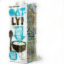
\includegraphics[width=\textwidth]{PaperA/decoded-image-figure/densenet_nov11/Oatly-Natural-Yoghurt_decoded.png}
		%\vspace{-7mm}
		\caption{}
		\label{subfig:oatgurt-decoded}
	\end{subfigure} ~~~
	\begin{subfigure}[b]{0.18\textwidth}
		\centering
		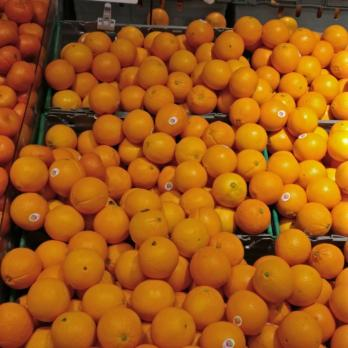
\includegraphics[width=\textwidth]{PaperA/decoded-image-figure/Orange_056.jpg}
		%\vspace{-7mm}
		\caption{}
		\label{subfig:orange-natural}
	\end{subfigure} ~
	\begin{subfigure}[b]{0.18\textwidth}
		\centering
		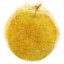
\includegraphics[width=\textwidth]{PaperA/decoded-image-figure/densenet_nov11/Orange_decoded.png}
		%\vspace{-7mm}
		\caption{}
		\label{subfig:orange-decoded}
	\end{subfigure} \\[1mm]
	\begin{subfigure}[b]{0.18\textwidth}
		\centering
		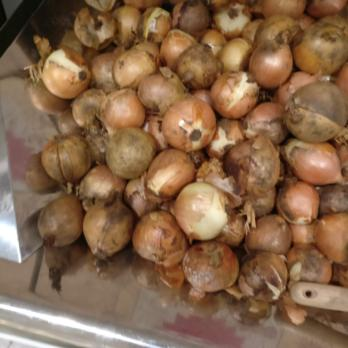
\includegraphics[width=\textwidth]{PaperA/decoded-image-figure/Yellow-Onion_030.jpg}
		%\vspace{-7mm}
		\caption{}
		\label{subfig:onion-natural}
	\end{subfigure} ~
	\begin{subfigure}[b]{0.18\textwidth}
		\centering
		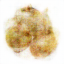
\includegraphics[width=\textwidth]{PaperA/decoded-image-figure/densenet_nov11/Yellow-Onion_decoded.png}
		%\vspace{-7mm}
		\caption{}
		\label{subfig:onion-decoded}
	\end{subfigure} ~~~
	\begin{subfigure}[b]{0.18\textwidth}
		\centering
		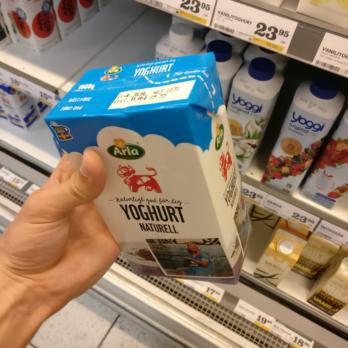
\includegraphics[width=\textwidth]{PaperA/decoded-image-figure/Arla-Natural-Yoghurt_014.jpg}
		%\vspace{-7mm}
		\caption{}
		\label{subfig:yogurt-natural}
	\end{subfigure} ~
	\begin{subfigure}[b]{0.18\textwidth}
		\centering
		\includegraphics[width=\textwidth]{PaperA/decoded-image-figure/densenet_nov11/Arla-Natural-Yoghurt_decoded.png}
		%\vspace{-7mm}
		\caption{}
		\label{subfig:yogurt-decoded}
	\end{subfigure}
	\vspace{-2mm}
	\caption{ 
	Examples of six natural images in the test set that have been decoded into product iconic images by the iconic image decoder $p_{\boldsymbol{\theta^{(2)}}}(\mathbf{y}\,|\,\mathbf{z})$ using VAE-CCA model as in Figure \ref{subfig:vae-cca}. This result is obtained with the fine-tuned DenseNet-169 features, which corresponds to VAE-CCA+SVM-ft in Table \ref{tab:results-fine-grained}. 
	We show the natural image and corresponding decoded iconic image next to each other. The classes for all images are (a, b) Royal Gala Apple, (c, d) Brown Cap Mushroom, (e, f) Oatly Oatgurt, (g, h) Orange, (i, j) Onion, and (k, l) Arla Natural Yogurt.
	%Examples of natural images in the test set that have been decoded into product iconic images by the iconic image decoder. This result is obtained with the fine-tuned DenseNet-169 features, which corresponds to VAE-CCA+SVM-ft in Table \ref{tab:results-fine-grained}. 
	%Subfigures (a), (c), (e), (g), (i) and (k) show the example input image from the test set, and Subfigures (b), (d), (f), (h), (j) and (l) show the decoded iconic image from the decoder $p_{\boldsymbol{\theta^{(2)}}}(\mathbf{y}\,|\,\mathbf{z})$ using VAE-CCA model as in Figure \ref{subfig:vae-cca}.
} 
	\label{fig:decoded-images}
\end{figure}

\begin{comment}
	
\begin{figure}[t]
\centering
\subfigure[Royal Gala]{\label{subfig:royal-gala-natural}\includegraphics[width=0.33\columnwidth]{PaperA/decoded-image-figure/Royal-Gala-Apple_003.jpg}}~
\subfigure[Decoded Royal Gala]{\label{subfig:royal-gala-decoded}\includegraphics[width=0.33\columnwidth]{PaperA/decoded-image-figure/densenet_nov11/Royal-Gala-Apple_decoded.png}}~
\subfigure[Brown Cap]{\label{subfig:brown-cap-natural}\includegraphics[width=0.33\columnwidth]{PaperA/decoded-image-figure/Mushroom-Brown-Cap_027.jpg}}~
\subfigure[Decoded\,Brown\,Cap]{\label{subfig:brown-cap-decoded}\includegraphics[width=0.33\columnwidth]{PaperA/decoded-image-figure/densenet_nov11/Mushroom-Brown-Cap_decoded.png}}~
\subfigure[Oatgurt]{\label{subfig:oatgurt-natural}\includegraphics[width=0.33\columnwidth]{PaperA/decoded-image-figure/Oatly-Natural-Yoghurt_007.jpg}}~
\subfigure[Decoded Oatgurt]{\label{subfig:oatgurt-decoded}\includegraphics[width=0.33\columnwidth]{PaperA/decoded-image-figure/densenet_nov11/Oatly-Natural-Yoghurt_decoded.png}}~ \\
\subfigure[Orange]{\label{subfig:orange-natural}\includegraphics[width=0.33\columnwidth]{PaperA/decoded-image-figure/Orange_056.jpg}}~
\subfigure[Decoded Orange]{\label{subfig:orange-decoded}\includegraphics[width=0.33\columnwidth]{PaperA/decoded-image-figure/densenet_nov11/Orange_decoded.png}}~
\subfigure[Onion]{\label{subfig:onion-natural}\includegraphics[width=0.33\columnwidth]{PaperA/decoded-image-figure/Yellow-Onion_030.jpg}}~
\subfigure[Decoded Onion]{\label{subfig:onion-decoded}\includegraphics[width=0.33\columnwidth]{PaperA/decoded-image-figure/densenet_nov11/Yellow-Onion_decoded.png}}~
\subfigure[Yogurt]{\label{subfig:yogurt-natural}\includegraphics[width=0.33\columnwidth]{PaperA/decoded-image-figure/Arla-Natural-Yoghurt_014.jpg}}~
\subfigure[Decoded Yogurt]{\label{subfig:yogurt-decoded}\includegraphics[width=0.33\columnwidth]{PaperA/decoded-image-figure/densenet_nov11/Arla-Natural-Yoghurt_decoded.png}}~
\caption{ Examples of natural images in the test set that have been decoded into product iconic images by the iconic image decoder. This result is obtained with the fine-tuned DenseNet-169 features, which corresponds to VAE-CCA+SVM-ft in Table \ref{tab:results-fine-grained}. Subfigures (a), (c), (e), (g), (i) and (k) show the example input image from the test set, and Subfigures (b), (d), (f), (h), (j) and (l) show the decoded iconic image from the decoder $p_{\boldsymbol{\theta^{(2)}}}(\mathbf{y}\,|\,\mathbf{z})$ using VAE-CCA model as in Figure \ref{subfig:vae-cca}.} \label{fig:decoded-images}
\end{figure}
\end{comment}

The fine-grained classification results for all methods using an SVM as classifier are shown in Table \ref{tab:results-fine-grained}. We also provide coarse-grained classification results for some of the methods in Table \ref{tab:results-coarse-grained} to demonstrate the possibility of hierarchical evaluation that our labeling of the data provides (see Figure \ref{fig:examples}). The accuracies in the coarse-grained classification are naturally higher than the accuracies in the corresponding columns in Table \ref{tab:results-fine-grained}. Table \ref{tab:results-finetuned-cnn} shows fine-grained classification accuracies from a softmax classifier in the fine-tuned CNNs. We note that fine-tuning the networks gives consistently better results than training an SVM on off-the-shelf features (see Table \ref{tab:results-fine-grained}).

Fine-tuning the entire network results improves the classification performance consistently for each method in Table \ref{tab:results-fine-grained}. The performance is clearly enhanced for features extracted from fine-tuned VGG16 and DenseNet-169, which improves the classification accuracy by 10\% in most cases for SVM-ft, VAE+SVM-ft, and VAE-CCA+SVM-ft. For AlexNet and VGG16, we see that the performance drops when extracting the features from layer FC7 instead of FC6. The reason might be that the off-the-shelf features in FC7 are more difficult to transfer to other datasets since the weights are biased towards classifying objects in the ImageNet database. The performance drops also when we use fine-tuned features, which could be due to the small learning rate we use for the pretrained layers, such that the later layers are still ImageNet-specific. We might circumvent this drop by increasing the learning rate for the later pretrained layers and keeping the learning rate for earlier layers small.
 
The VAE-CCA model achieves mostly higher classification accuracies than the VAE model in both Table \ref{tab:results-fine-grained} and \ref{tab:results-coarse-grained}. This indicates that the latent representation separates the classes more distinctly than the VAE by jointly learning to reconstruct the extracted feature vectors and iconic images. However, further compressing the feature vectors with VAE and VAE-CCA will lower the classification accuracy compared to applying the feature vectors to a classifier directly. Since both VAE and VAE-CCA compresses the feature vectors into the latent representation, there is a risk of losing information about the natural images. We might receive better performance by increasing the dimension of the latent representation at the expense of speed in both training and classification.

In Figure \ref{fig:decoded-images}, we show results from the iconic image decoder $p_{\boldsymbol{\theta^{(2)}}}(\mathbf{y}\,|\,\mathbf{z})$ when translating natural images from the test set into iconic images with VAE-CCA and a fine-tuned DenseNet-169 as feature extractor. Such visualization can demonstrate the quality of the representation using the model, as well as enhancing the interpretability of the method. Using VAE-CCA in the proposed manner, we see that with challenging natural images, the model is still able to learn an effective representation which can be decoded to the correct iconic image. For example, some pears have been misplaced in the bin for Royal Gala apples in Figure \ref{subfig:royal-gala-natural}, but still the image decoder manages to decode a blurry red apple seen in Figure \ref{subfig:royal-gala-decoded}. In Figure \ref{subfig:orange-decoded}, a mix of an orange and an apple are decoded from a bin of oranges in Figure \ref{subfig:orange-natural}, which indicates these fruits are encoded close to each other in the learned latent space. Even if Figure \ref{subfig:oatgurt-natural} includes much of the background, the iconic image decoder is still able to reconstruct the iconic images accurately in Figure \ref{subfig:oatgurt-decoded}, which illustrates that the latent representation is able to explain away irrelevant information in the natural image and preserved the features of the oatgurt package. Thus, using VAE-CCA with iconic images as the second view not only advances the classification accuracy but also provides us with the means to understand the model.



\section{Conclusions}\label{paperA:sec:conclusions}

This paper presents a dataset of images of various raw and packaged grocery items, such as fruits, vegetables, and dairy and juice products. We have used a structured labeling of the items, such that grocery items can be grouped into more general (coarse-grained) classes and also divided into fine-grained classes. For each class, we have a clean iconic image and a text description of the item, which can be used for adding visual and semantic information about the items in the modeling. The intended use of this dataset is to train and benchmark assistive systems for visually impaired people when they shop in a grocery store. Such a system would complement existing visual assistive technology, which is confined to grocery items with barcodes. We also present preliminary benchmark results for the dataset on the task of image classification. 

We make the dataset publicly available for research purposes at \url{https://github.com/marcusklasson/GroceryStoreDataset}. Additionally, we will both continue collecting natural images, as well as ask for public contributions of natural images in shopping scenarios to enlarge our dataset. 

For future research, we will advance our model design to utilize the structured nature of our labels. Additionally, we will design a model that use the product description of the objects in addition to the iconic images. One immediate next step is to extend the current VAE-CCA model to three views, where the third view is the description of the product. 




\renewcommand*{\bibname}{References}
\bibliographystyleA{unsrt}
\bibliographyA{References/paperA_test}

\cleardoublepage


%%% Paper B %%%
%\renewcommand*{\thepage}{B\arabic{page}}
%\setcounter{page}{1}
\setcounter{section}{0}


%\renewcommand*{\bibname}{References}
%\renewcommand*{\thechapter}{B}  % use A, B, C for chapter numbers
%\renewcommand{\chaptername}{Paper} % A chapter is now called Paper
%\renewcommand\thesection{\arabic{section}}
%\renewcommand*{\thepage}{B\arabic{page}}
%\setcounter{page}{1}

%%% Paper content

\chapter{
	\centering{Using Variational Multi-View Learning for Classification of Grocery Items}
}\label{paperB}
\chaptermark{Variational Multi-View Learning for Grocery Classification}
\vspace{-5mm}
\begin{center}
	\large{\textbf{Marcus Klasson$^{*}$, Cheng Zhang$^{\dagger}$, Hedvig Kjellström$^{*}$}} \\[2mm]
	\small{$^{*}$KTH Royal Institute of Technology, Stockholm, Sweden} \\
	\small{$^{\dagger}$Microsoft Research, Cambridge, United Kingdom} \\
\end{center}


%%%%%%%%%%%%%%%%%%%%%%%%%%%%%%%%%%%%%%%%%%%%%%%%%%%%%%%%%%%%%%%%%%%%%%%%%%%%%%%%
%%%%%%%%%%%%%%%%%%%%%%%%%%%%%%%%%%%%%%%%%%%%%%%%%%%%%%%%%%%%%%%%%%%%%%%%%%%%%%%%
\begin{abstract}
	%\printinunitsof{in}\prntlen{\linewidth}
	\noindent An essential task for computer vision-based assistive technologies is to help visually impaired people to recognize objects in constrained environments, for instance, recognizing food items in grocery stores. In this paper, we introduce a novel dataset with natural images of groceries -- fruits, vegetables, and packaged products -- where all images have been taken inside grocery stores to resemble a shopping scenario. Additionally, we download iconic images and text descriptions for each item that can be utilized for better representation learning of groceries. We select a multi-view generative model, which can combine the different item information into lower-dimensional representations. The experiments show that utilizing the additional information yields higher accuracies on classifying grocery items over only using the natural images. We observe that iconic images help to construct representations separated by visual differences of the items, while text descriptions enable the model to distinguish between visually similar items by different ingredients.
\end{abstract}

%%% Contents
\section{Introduction}
\label{paperB:sec:introduction}

%\renewcommand{\thefootnote}{\fnsymbol{footnote}}
In recent years, computer vision-based assistive technologies have been developed for supporting people with visual impairments.
Such technologies exist in the form of mobile applications, e.g., Microsoft's Seeing AI~\citeB{B:seeingAImicrosoft} and Aipoly Vision~\citeB{B:aipolyvision}, and as wearable artificial vision devices, e.g., Orcam MyEye~\citeB{B:orcam}, Transsense~\citeB{B:transsense}, and the Sound of Vision system~\citeB{B:caraiman2017soundofvision}. These products can support people with visual impairments in many different situations, such as reading text documents, describing the user's environment, and recognizing people the user may know. 
%Such technologies exist in the form of mobile applications, e.g., Microsoft's Seeing AI ({\small \url{https://www.microsoft.com/en-us/seeing-ai/}}) and Aipoly Vision ({\small \url{https://www.aipoly.com/}}), and as wearable artificial vision devices, e.g., Orcam MyEye ({\small \url{https://www.orcam.com/en/}}), Transsense ({\small \url{https://www.transsense.ai/}}), and the Sound of Vision system~\citeB{caraiman2017soundofvision}. These products can support people with visual impairments in many different situations, such as reading text documents, describing the user's environment, and recognizing people the user may know. 
In this paper, we focus on an application that is essential for assistive vision, namely visual support when shopping for grocery items considering a large range of eatable objects, including fruits, vegetables, and refrigerated products, e.g., milk and juice packages.

Grocery shopping with low vision capabilities can be difficult for various reasons. For example, in grocery store sections for raw groceries, the items are often stacked in large bins as shown in Figure \ref{fig:dataset_figures}(a-f). Additionally, similar items are usually stacked next to each other, and therefore, items are can be misplaced into neighboring bins. Humans can distinguish between groceries without vision to some degree, e.g., by touch and smell, but it requires prior knowledge about texture and fragrance of food items. 
Furthermore, packaged items, e.g., milk, juice, and yoghurt cartons, can only be differentiated with the help of visual information (see Figure \ref{fig:dataset_figures}(g-i)). 
Such items usually have barcodes, that are readable using the existing assistive vision devices described above. 
Even if using a barcode detector is a clever solution, it can be inconvenient and exhausting always having to detect barcodes of packaged items.
Therefore, an assistive vision device that relies on natural images would be of significant value for a visually impaired person in a grocery store. 

%%% Figure 1 and 2


\begin{figure}[t] 
	\centering
	\begin{minipage}[b]{0.47\textwidth}
    	\includegraphics[scale=0.5]{PaperB/figures_and_tables/figure1.png}
		\caption{Examples of natural images in our dataset, where each image has been taken inside a grocery store. Image examples of fruits, vegetables, and refrigerated products are presented in each row respectively.}
		\label{fig:dataset_figures}
	\end{minipage}
	\hspace{10pt}
	%\vspace{-10mm}
	\begin{minipage}[b]{0.47\textwidth}
		\centering
	    \includegraphics[scale=0.5]{PaperB/figures_and_tables/figure2.png}
		\caption{Examples of iconic images downloaded from a grocery shopping website, which corresponds to the target items in the images in Figure \ref{fig:dataset_figures}. \newline}
		\label{fig:iconic_image_figures}
	\end{minipage} 
	\vspace{-2mm}
\end{figure}



\begin{comment}

\begin{figure}
    \centering
    \includegraphics[scale=0.5]{PaperB/figures_and_tables/figure1.png}
    \caption{Examples of natural images in our dataset, where each image has been taken inside a grocery store. Image examples of fruits, vegetables, and refrigerated products are presented in each row respectively.}
    \label{fig:dataset_figures}
\end{figure}

\begin{figure}
    \centering
    \includegraphics[scale=0.5]{PaperB/figures_and_tables/figure2.png}
    \caption{Examples of iconic images downloaded from a grocery shopping website, which corresponds to the target items in the images in Figure \ref{fig:dataset_figures}.}
    \label{fig:iconic_image_figures}
\end{figure}.
\end{comment}



For an image classification model to be capable of recognizing grocery items in the setting of grocery shopping, we need image data from grocery store environments. 
In our previous work~\citeB{B:klasson2019hierarchical}, we addressed this by collecting a novel dataset containing natural images of various raw grocery items and refrigerated products, where all images have been taken with a smartphone camera inside grocery stores to simulate a realistic shopping scenario.
In addition to the natural images, we also looked upon alternative types of grocery item data that could facilitate the classification task.
Grocery store chains commonly maintain websites where they store information about the grocery items they sell and are currently available in the store for online grocery shopping. 
For every item, there is usually an iconic image of the item with white background, a text description about the item, and also information about nutrition values, origin country, etc.
We downloaded such information from an online grocery shopping website to complement the natural images in the dataset.

To utilize the available information from the dataset for grocery item classification, we use a multi-view generative model Variational Canonical Correlation Analysis (VCCA)~\citeB{B:wang2016deep} that learns a shared representation of the natural images and the downloaded information. A view can be defined as any signal or data measured by some appropriate sensor and combining information from multiple views has previously been shown to be helpful for various image classification tasks~\citeB{B:donahue2015long-term, B:frome2013DeVISE, B:karpathy2015deep, B:kulkarni2013babytalk, B:lu2018neural, B:lu2016hierarchical, B:parikh2011relative, B:srivastava2014multimodal}. However, naively adding more additional information may not lead to improved results and even harm the performance of the model~\citeB{B:guler2014whats,B:ngiam2011multimodal}. We, therefore, perform an ablation study over the available views in the dataset with VCCA to gain insights into how each view can affect the classification performance. Moreover, VCCA allows separating the latent space into shared and private components, where the private latent spaces should hold information about a single view. This might prove useful for reducing view-specific noise in the shared latent space, which can ease the learning process of the representations we want to use for classification. We investigate the effects each view has on the learned representations of VCCA by measuring classification performances as well as visualizing the latent space for the different model settings. The contributions of this paper are the following:

\begin{itemize}[topsep=1pt, leftmargin=*] 
    \item We present a novel dataset with natural images of grocery items as well as iconic images and text descriptions for every item class (see Section 
    %subsection The Grocery Store Dataset in Results)~\citeB{B:klasson2019hierarchical}.
    \ref{paperB:sec:grocery_store_dataset})~\citeB{B:klasson2019hierarchical}.
    The natural images are taken in grocery stores in different lighting conditions and backgrounds that can be challenging settings for a computer vision-based assistive device. The additional iconic images and text descriptions make the dataset suitable for multi-view learning by combining the natural images with the extra information to obtain better classification performance.  
    
    \item We investigate how to use information from different views for the task of grocery item classification with the deep generative model VCCA (see Section \ref{paperB:sec:methods}). %subsection Methods in Experimental Procedures).
    %\ref{sec:methods}).
    This model combines information from multiple views into a low-dimensional latent representation that can be used for classification. We also select a variant of VCCA denoted VCCA-private that separates shared and private information about each view through factorization of the latent representation (see subsection Extracting Private Information of Views with VCCA-private in Experimental Procedures). 
    %\ref{sec:extracting_private_information}). 
    Furthermore, we use a standard multi-view autoencoder model called Split Autoencoder (SplitAE)~\citeB{B:ngiam2011multimodal, B:wang2015deep} for benchmarking against VCCA and VCCA-private on classification.
    
    \item We conduct experiments with SplitAE, VCCA, and VCCA-private on the task of grocery item classification with our dataset (Results).
    %Section \ref{sec:results}).
    We perform a thorough ablation study over all views in the dataset to demonstrate how each view contributes to enhancing the classification performance and conclude that utilizing the web-scraped views yields better classification results than only using the natural images (see subsection Classification Results in Results).
    % Section \ref{sec:classification_results}). 
    To gain further insights into the results, we visualize the learned latent representations of the VCCA models and discuss how the iconic images and textual descriptions impose different structures on the latent space that are beneficial for classification (see subsection Investigation of the Learned Representations in Results).
    %Section \ref{sec:investigation_of_the_learned_representations}). 
    
\end{itemize}
This work is an extended version of Klasson \etal~\citeB{B:klasson2019hierarchical}, where we first presented this dataset. In this paper, we have added a validation set of natural images from two stores that were not present in the training and test set splits from \citeB{B:klasson2019hierarchical} to avoid overfitting effects. We also demonstrate how the text descriptions can be utilized alone and along with the iconic images in a multi-view setting, while \citeB{B:klasson2019hierarchical} only experimented with the combination of natural and iconic images to build better representations of grocery items. Finally, we decode iconic images from unseen natural images as an alternative to evaluate the usefulness of the latent representations (see subsection Decoding Iconic Images from Unseen Natural Images in Results).
%(see Section \ref{sec:decoding_iconic_images}). 
As we only evaluated the decoded iconic images qualitatively in Klasson \etal~\citeB{B:klasson2019hierarchical}, we have extended the assessment by comparing the quality of the decoded images from different VCCA models with multiple image similarity metrics. 

%% RELATED WORK
Next, we discuss image datasets, food datasets, and multi-view models related to our work:

\vspace{-3mm}
\paragraph{Image Datasets} Many image datasets used in computer vision have been collected by downloading images from the web \citeB{B:deng2009imagenet, B:everingham2010pascal, B:gebru2017finegrained, B:griffin2007caltech256, B:krishna2016visualgenome, B:Krizhevsky2009cifar100, B:Lin2014MicrosoftCoco, B:nilsback2008flowers, B:song2016deep, B:WahCUB_200_2011, B:xiao2010sundatabase, B:young2014flickr30k}. 
Some datasets~\citeB{B:deng2009imagenet, B:griffin2007caltech256, B:Krizhevsky2009cifar100, B:nilsback2008flowers, B:WahCUB_200_2011} use search words with the object category in isolation, which typically returns high-quality images where the searched object is large and centered. To collect images from more real-world scenarios, searching for combinations of object categories usually returns images of two searched categories but also numerous other categories~\citeB{B:Lin2014MicrosoftCoco, B:young2014flickr30k}. 
The simplest annotation of these images is to provide a class label for the present objects. Occasionally, the dataset can use a hierarchical labeling structure and provide a fine- and coarse-grained label to objects where it is applicable. 
The annotators can also be asked to increase the possible level of supervision for the objects by, for instance, providing bounding boxes, segmentation masks, keypoints, text captions that describe the scene, and reference images of the objects~\citeB{B:gebru2017finegrained, B:krishna2016visualgenome, B:Lin2014MicrosoftCoco, B:nilsback2008flowers, B:WahCUB_200_2011, B:young2014flickr30k}. Our dataset includes reference (iconic) images of the objects that were web-scraped from a grocery store website. We also downloaded text descriptions that describe general attributes of the grocery items, such as flavor and texture, rather than the whole visual scene. The grocery items have also been labeled hierarchically in a fine- and coarse-grained manner if there exist multiple variants of specific items. For example, fine-grained classes of apples such as \textit{Golden Delicious} or \textit{Royal Gala} belongs to the coarse-grained class \textit{apple}.

\vspace{-3mm}
\paragraph{Food Datasets} 
Recognizing grocery items in their natural environments, such as grocery stores, shelves, and kitchens, have been addressed in plenty of previous works \citeB{B:geng2018fine, B:george2014recognizing, B:hsiao2010making, B:jund2016freiburg, B:klasson2019hierarchical, B:lai2011large, B:merler2007recognizing, B:singh2014bigbird, B:waltner2015mango, B:wei2019rpc, B:winlock2010toward, B:yu2018take}. The addressed tasks range from hierarchical classification, object detection, segmentation, and 3D model generation. Most of these works collect a dataset that resembles shopping or cooking scenarios, where the datasets vary in the degree of labeling, different camera views, and the data domain difference between the training and test set. 
The training sets in GroZi-120~\citeB{B:merler2007recognizing}, Grocery Products~\citeB{B:george2014recognizing}, and CAPG-GP~\citeB{B:geng2018fine} datasets were obtained by web-scraping product images of single instances on grocery web stores, while the test sets were collected in grocery stores where there can be single and multiple instances of the same item and other different items.
The RPC~\citeB{B:wei2019rpc} and TGFS~\citeB{B:yu2018take} datasets are used for object detection and classification of grocery products, where RPC is targeted for automatic checkout systems and TGFS is for the task of recognizing items purchased from self-service vending machines.
The BigBIRD~\citeB{B:singh2014bigbird} dataset and datasets from~\citeB{B:hsiao2010making, lai2011large} contain images of grocery items from multiple camera views, segmentation masks, and depth maps for 3D reconstruction of various items. 
The Freiburg Groceries~\citeB{B:jund2016freiburg} dataset contains images taken with smartphone cameras of items inside grocery stores, while its test set consists of smartphone photos in home environments with single or multiple instances from different kinds of items. The dataset presented in~\citeB{B:waltner2015mango} also contains images taken with smartphone cameras inside grocery stores to develop a mobile application for recognizing raw food items and provide details about the item, such as nutrition values and recommendations of similar items. Other works that collected datasets of raw food items, such as fruits and vegetables, focused on the standard image classification task~\citeB{B:muresan2017fruit, B:marko2013fids30} and on detecting fruits in orchards for robotic harvesting~\citeB{B:bargoti2017deepfruitdetection, B:sa2016deepfruits}. Our dataset -- the Grocery Store dataset -- shares many similarities with the mentioned works above, for instance, that all images of groceries are taken in their natural environment, the hierarchical labeling of the classes, and the iconic product images for each item in the dataset. Additionally, we have provided a text description for each item that was web-scraped along with the iconic image. As most grocery item datasets only include packaged products, we have also collected images of different fruit and vegetable classes along with packages in our dataset. 

Other examples of food datasets are those with images of food dishes, where \citeB{B:min2019survey} provides a summary of existing benchmark food datasets. The contents of these datasets range from images of food dishes~\citeB{B:bossard2014food101, B:kawano2014automatic, B:min2019ingredient, B:rich2016towards}, cooking videos~\citeB{B:damen2018scaling}, recipes~\citeB{B:marin2019learning, B:salvador2017learning, B:yagcioglu2018recipeqa}, and also restaurant-oriented information~\citeB{B:beijbom2015menu, B:xu2015geolocalized}. One major difference between recognizing groceries and food dishes is the appearance of the object categories in the images. For instance, a fruit or vegetable is usually intact and present in the image, while ingredients that are significant for recognizing a food dish may not be visible at all depending on the recipe. However, recognizing raw food items and dishes share similarities since they can appear with many different visual features in the images compared to packaged groceries, e.g., carton boxes, cans, and bottles, where the object classes have identical shape and texture. 
Another key difference is the natural environments and scenes where the images of grocery items and food dishes have been taken. Food dish images usually show the food on a plate placed on a table and, occasionally, with cutlery and a glass next to the plate. Images taken in grocery stores can cover many instances of the same item stacked close to each other in shelves, baskets, and refrigerators, while there can be multiple different kinds of items next to each other in a kitchen environment. 
To summarize, recognizing grocery items and food dishes are both challenging tasks because examples from the same category can look very different and also appear in various realistic settings in images.

\vspace{-3mm}
\paragraph{Multi-View Learning Models} There exist lots of multi-view learning approaches for data fusion of multiple features~\citeB{B:baltruvsaitis2018multimodal, B:cremer2018importance, B:frome2013DeVISE, B:fu2016semi, B:karpathy2015deep, B:ngiam2011multimodal, B:pieropan2014audio,  B:salzmann2010factorized, B:shi2019variational, B:suzuki2016joint, B:tsai2018learning, B:vedantam2017generative, B:wang2016deep, B:wu2018multimodal, B:xian2018zero, B:xu2013survey, B:zhang2016inter, B:zhao2017multi}. A common approach is to obtain a shared latent space for all views with the assumption that each view has been generated from this shared space~\citeB{B:xu2013survey}. A popular example of this is approach is Canonical Correlation Analysis (CCA)~\citeB{B:hotelling1936relations}, which aims to project two sets of variables (views) into a lower-dimensional space so that the correlation between the projections is maximized. Similar methods propose maximizing other alignment objectives for embedding the views, such as ranking losses~\citeB{B:frome2013DeVISE, B:fu2016semi, B:karpathy2015deep, B:xian2018zero}. 
There exist nonlinear extensions of CCA, e.g., Kernel CCA~\citeB{B:akaho2006kernel} and Deep CCA~\citeB{B:andrew2013deep}, that optimize their nonlinear feature mappings based on the CCA objective. 
Deep Canonically Correlated Autoencoders (DCCAE)~\citeB{B:wang2015deep} is a Deep CCA model with an autoencoding part, which aims to maximize the canonical correlation between the extracted features as well as reconstructing the input data. 
Removing the CCA objective reduces DCCAE to a standard multi-view autoencoder, e.g., Bimodal Autoencoders and Split Autoencoders (SplitAEs)~\citeB{B:ngiam2011multimodal, B:wang2015deep}, that only aim to learn a representation that best reconstructs the input data. SplitAEs aim to reconstruct two views from a representation encoded from one of the views. This approach was empirically shown to work better than Bimodal Autoencoders in \citeB{B:ngiam2011multimodal} in situations where only a single view is present at both training and test time.

Variational CCA (VCCA)~\citeB{B:wang2016deep} can be seen as an extension of CCA to deep generative models, but can also be described as a probabilistic version of SplitAEs.
VCCA uses the amortized inference procedure from Variational Autoencoders (VAEs)~\citeB{B:kingma2013auto, B:zhang2018advances} to learn the shared latent space by maximizing a lower bound on the data log-likelihood of the views. Succeeding works have proposed new learning objectives and inference methods for enabling conditional generation of views, e.g., generating an image conditioned on some text and vice versa~\citeB{B:cremer2018importance, B:shi2019variational, B:suzuki2016joint, B:vedantam2017generative, B:wu2018multimodal}. These approaches rely on fusing the views into the shared latent space as the inference procedure, which often requires tailored training and testing paradigms when views are missing. However, adding information from multiple views may not lead to improved results and can even make the model perform worse on the targeted task~\citeB{B:guler2014whats, B:ngiam2011multimodal}. This is especially the case when views have noisy observations, which complicates learning a shared latent space that combines the commonalities between the views. To avoid disturbing the shared latent space with noise from single views, some works design models which extend the shared latent space with private latent spaces for each view that should contain the view-specific variations to make learning the shared variations easier~\citeB{B:hyvarinen2000independent, B:salzmann2010factorized, B:tsai2018learning, B:wang2016deep, B:zhang2016inter}. VCCA can be extended to extract shared and private information between different views through factorization of the latent space into shared and private parts. In this paper, we investigate if the classification performance of grocery items in natural images can be improved by extracting the view-specific variations in the additional views (iconic images and product descriptions) from the shared latent space with this variant of VCCA called VCCA-private. We will experiment with treating each data point as pairs of natural images and either iconic images or text descriptions as well as triplets of natural images, iconic images, and text descriptions.
A difference between how we apply VCCA to our dataset compared to the works above is that the iconic image and text description are the same for every natural image of a specific class.  




\section{Results}\label{paperB:sec:results}

In this section, we begin by providing the details about the collected dataset, which we have named the Grocery Store dataset. Furthermore, we illustrate the utility of the additional information in the Grocery Store dataset to classify grocery items in the experiments. We compare SplitAE, VCCA, and VCCA-private with different combinations of views against two standard image classifiers. Additionally, we experiment with a vanilla autoencoder (denoted as AE) and a VAE that post-processes the natural image features to train a linear classifier cheaper and compare the performance against the multi-view models. We measure the classification performance on the test set for every model and also compare the classification accuracies when the number of words in the text description varies for the models concerned (see subsection Classification Results in Results).
%(Section \ref{sec:classification_results}).
To gain insights on how the additional views affect the learned representations, we visualize the latent spaces of VCCA and VCCA-private with PCA and discuss how different views changes the structure of the latent space (see subsection Investigation of the Learned Representations in Results).
%(Section \ref{sec:investigation_of_the_learned_representations}).
Finally, we show how iconic images can be used for enhancing the interpretability of the classification (see subsection Decoding Iconic Images from Unseen Natural Images in Results),
%(Section \ref{sec:decoding_iconic_images}), 
which was also illustrated by Klasson \etal~\citeB{B:klasson2019hierarchical}.


\subsection{The Grocery Store Dataset}
\label{paperB:sec:grocery_store_dataset}

%%% Figure 3

\begin{figure}[t]
    \centering
    \includegraphics[width=\textwidth]{PaperB/figures_and_tables/dataset_figures/dataset_figure_new.pdf} %\includegraphics[width=0.95\textwidth]{dataset_figures/intro.pdf}
    \vspace{-2mm}
    \caption{Illustration of the hierarchical class structure of the dataset. First, the classes are divided by their grocery item type, i.e., \textit{Fruits}, \textit{Vegetables}, and \textit{Packages}, followed by a separating the items into coarse-grained classes, e.g., \textit{Apple}, \textit{Carrot}, and \textit{Milk}, and then into fine-grained classes. There are 81 fine-grained classes in total and 46 coarse-grained classes. The figure also shows the iconic image and text description of the items next to the class label.
   }
    \label{fig:examples} 
\end{figure}

In Klasson \etal~\citeB{B:klasson2019hierarchical}, we collected images from fruit, vegetable, and refrigerated sections with dairy and juice products in 20 different grocery stores.
The dataset consists of 5421 images from 81 different classes. For each class, we have downloaded an iconic image of the item, a text description, and information including origin country, appreciated weight and nutrient values of the item from a grocery store website. Some examples of natural images and downloaded iconic images can be seen in Figure \ref{fig:dataset_figures} and \ref{fig:iconic_image_figures} respectively. Furthermore, Table S1 displays a selection of text descriptions with their corresponding iconic image. 
The text description length varies between 6 and 91 words with an average of 36 words. 
We also structure that classes hierarchically with three levels as illustrated in Figure \ref{fig:examples_paperB}. The first level divides the items into three categories; \textit{Fruits}, \textit{Vegetables}, and \textit{Packages}. The next level consists of 46 coarse-grained classes which divides the items into groups contain groups of items types, e.g., \textit{Apple}, \textit{Carrot}, \textit{Milk}. The bottom level consists of the 81 fine-grained classes, where the items are completely separated. Note that a coarse-grained class without any fine-grained classes in the dataset, e.g., \textit{Banana} and \textit{Carrot}, is considered as a fine-grained class in the classification experiments (see subsection Classification Results in Results),
%(see Section \ref{sec:classification_results}), 
where we report both fine-grained and coarse-grained classification performance of the models.

We aimed to collect the natural images under similar conditions as if they would be taken with an assistive mobile application. 
All images have been taken with a 16-megapixel Android smartphone camera from different distances and angles. 
Occasionally, the images include other items in the background or even items that have been misplaced in incorrect shelves along with the targeted item.
The lighting conditions in the images can also vary depending on where the items are located in the store. Sometimes the images are taken while the photographer is holding the item in the hand. This is often the case for refrigerated products since these containers are usually stacked compactly in the refrigerators. For these images, we have consciously varied the position of the object, such that the item is not always centered in the image or present in its entirety. We split the natural images into a training set and test set based on the application need. Since the images have been taken in several different stores at specific days and time stamps, parts of the data will have similar lighting conditions and backgrounds for each photo occasion. To remove any such biasing correlations, all images of a certain class taken at a certain store are assigned to either the training set, validation set, or test set. In the first version of the dataset~\citeB{B:klasson2019hierarchical}, we balanced the class sizes to a large extent as possible in both the training and test set, which resulted in a training and test set containing 2640 and 2485 images respectively. In this paper, we have extended the dataset with a validation set containing 296 images taken with the same smartphone camera as before. The validation set was collected from two different grocery stores than the ones in the first version to avoid the biasing correlations described above. 
Initially, we experimented with grabbing a validation set from the current training set and noticed that the trained classifiers performed exceptionally well on the validation set. However, the classifiers generalized poorly to images from the test set that were taken in other stores and therefore decided to collect the validation set in two unseen stores to avoid the biases from the training set. We show histograms representing the class distributions for the training, validation, and test splits in Figure S1.

The scenario that we wanted to depict with the dataset was using a mobile device to classify natural images visually impaired people with grocery shopping. The additional information such as the iconic images, text descriptions, and hierarchical structure of the class labels can be used to enhance the performance of the computer vision system. Since every class label is associated with a text description, the description itself can be part of the output for visually impaired persons as they may not be able to read what is printed on a carton box or a label tag on a fruit bin in the store. 

\subsection{Models}

In this section, we briefly describe the models that we apply to grocery classification. The notation of the views that are available in the Grocery Store dataset are the following:
\begin{itemize}[topsep=1pt, noitemsep]%leftmargin=*] 
    \item $x$: Natural image encoded into image feature space with an off-the-shelf convolutional neural network.
    \item $i$: Iconic image of the object class in the natural image.
    \item $w$: Text description of the object class in the natural image.
    \item $y$: Class label of the natural image.
\end{itemize}
We mainly focus on analyzing VCCA~\citeB{B:wang2016deep} for utilizing different combinations of the views and investigate how each view contributes to the classification performance of grocery items. Our primary baseline model is the SplitAE which extracts shared representations by reconstructing all views, while VCCA aims to maximize a lower bound on the data log-likelihood for all views. We also study a variant of VCCA called VCCA-private~\citeB{B:wang2016deep}, which is used for extracting private information about each view in addition to shared information across all views by factorizing the latent space. 

We compare the multi-view models against single-view methods only using the natural images for classification. As our first single-view baseline, we customize the output layer of DenseNet169~\citeB{B:huang2017densely} to %our 
the Grocery Store dataset and train it from scratch to classify the natural images, which we refer to as DenseNet-scratch in the experiments. The second baseline called Softmax is a Softmax classifier trained on the off-the-shelf features from DenseNet169 pre-trained on the ImageNet dataset~\citeB{B:deng2009imagenet}, where we extract 1664-dimensional from the average pooling layer before the classification layer in the architecture. We also experiment with AEs and VAEs for post-processing the off-the-shelf features and use a linear classifier to evaluate the models on classification. See Section \ref{paperB:sec:methods} %subsection Methods in Experimental Procedures
%See Section \ref{sec:methods} 
for a thorough description of the single- and multi-view autoencoders used in this paper. We name the single- and multi-view autoencoders using subscripts to denote the views utilized for learning the shared latent representations. For example, VCCA$_{x i}$ utilizes natural image features $x$ and iconic images $i$, while VCCA$_{x i w y}$ uses natural image features $x$ and iconic images $i$, text descriptions $w$, and class labels $y$.


\subsection{Classification Results}
\label{paperB:sec:classification_results}

We evaluated the classification accuracy on the test set for each model. We also calculate the accuracy for the coarse-grained classes with the following method: Let the input $x^{(i)}$ have a fine-grained class $y_{fg}^{(i)}$ and a coarse-grained class $y_{cg}^{(i)}$. Each fine-grained class can be mapped to its corresponding coarse-grained class using $\parents(y_{fg}^{(i)}) = y_{cg}^{(i)}$, where $\parents(\cdot)$ stands for "parent". Then we compute the coarse-grained accuracy using  
\begin{align}\label{eq:coarse_accuracy}
    \begin{split}
        \text{coarse accuracy} & = \frac{1}{N} \sum_{i=1}^{N} \left[ \parents(\hat{y}_{fg}^{(i)}) = y_{cg}^{(i)} \right], \\ 
        \hat{y}_{fg}^{(i)} & = \argmax_{y} p(y | x^{(i)}),
    \end{split}
\end{align}
where $\left[ \parents(\hat{y}_{fg}^{(i)}) = y_{cg}^{(i)} \right] = 1$ when the condition is true and $\hat{y}_{fg}^{(i)}$ is the predicted fine-grained class from the selected classifier. The classification results for all models are shown in Table \ref{tab:classification_results_on_test_set}. We group the results in the table according to the utilized views and classifier. We see that Softmax trained on off-the-shelf features outperforms DenseNet-scratch by 4\%. This result is common when applying deep learning to small image datasets, where pre-trained deep networks are transferred to a new dataset usually performs well compared to training neural networks on the dataset from scratch. Therefore, we present results using the off-the-shelf features for all other models. 


\renewcommand{\arraystretch}{1.05}
\begin{table}[th!]
\centering
\caption{Classification accuracies on the test set for all models in percentage (\%) along for each model. The subscript letters in the model names indicate the data views used in the model. The column Accuracy corresponds to the fine-grained classification accuracy. The column Coarse Accuracy corresponds to the classifying a class within the correct parent class. Results are averaged using 10 different random seeds and we report both means and standard deviations. Abbreviations: AE, Autoencoder; VAE, Variational Autoencoder; SplitAE, Split Autoencoder; VCCA, Variational Canonical Correlation Analysis.
}
\begin{tabular}{l c c} 
    \hline 
    Model & Accuracy (\%) & Coarse Accuracy (\%) \\ 
    \hline
    DenseNet-scratch & $67.33 \pm \, 1.35$ & $75.67 \pm \, 1.15$ \\ 
    \rowcolor{gray!30}
    Softmax & $71.67 \pm 0.28$ & $83.34 \pm 0.32$ \\ 
    \hline
    AE$_{x}$+Softmax & $70.69 \pm 0.82$ & $82.42 \pm 0.58$ \\ 
    \rowcolor{gray!30}
    VAE$_{x}$+Softmax & $69.20 \pm 0.46$ & $81.24 \pm 0.63$ \\ 
    \hline
    SplitAE$_{x y}$ & $70.34 \pm 0.56$ & $82.11 \pm 0.38$ \\ 
    \rowcolor{gray!30}   
    VCCA$_{x y}$ & $70.72 \pm 0.56$ & $82.12 \pm 0.61$ \\ 
    \hline
    SplitAE$_{x i}$+Softmax & $77.68 \pm 0.69$ & $87.09 \pm 0.53$ \\ 
    \rowcolor{gray!30}  
    VCCA$_{x i}$+Softmax & $77.02 \pm 0.51$ & $86.46 \pm 0.42$ \\ 
    VCCA-private$_{x i}$+Softmax & $73.04 \pm 0.56$ & $84.16 \pm 0.51$ \\ \hline 
    \rowcolor{gray!30}
    SplitAE$_{x i y}$ & $77.43 \pm 0.80$ & $87.14 \pm 0.57$ \\ 
    VCCA$_{x i y}$ &  $77.22 \pm 0.55$ & $86.54 \pm 0.51$ \\ 
    \rowcolor{gray!30}  
    VCCA-private$_{x i y}$ & $74.04 \pm 0.83$ & $84.59 \pm 0.83$ \\
    \hline
    SplitAE$_{x w}$+Softmax & $76.27 \pm 0.66$ & $86.45 \pm 0.56$ \\
    \rowcolor{gray!30}  
    VCCA$_{x w}$+Softmax & $75.37 \pm 0.46$ & $86.00 \pm 0.32$\\
    VCCA-private$_{x w}$+Softmax & $75.11 \pm 0.81$ & $85.91 \pm 0.55$ \\ \hline
    \rowcolor{gray!30} 
    SplitAE$_{x w y}$ & $75.78 \pm 0.84$ & $86.13 \pm 0.63$ \\ 
    VCCA$_{x w y}$ & $74.72 \pm 0.85$ & $85.59 \pm 0.78$ \\ 
    \rowcolor{gray!30}  
    VCCA-private$_{x w y}$ & $74.92 \pm 0.74$ & $85.59 \pm 0.67$ \\
    \hline
    SplitAE$_{x i w}$+Softmax & $77.79 \pm 0.48$ & $87.12 \pm 0.62$ \\
    \rowcolor{gray!30}  
    VCCA$_{x i w}$+Softmax & $77.51 \pm \, 0.51$ & $86.69 \pm 0.41$ \\   
    \hline
    SplitAE$_{x i w y}$  & $78.18 \pm 0.53$ & $87.26 \pm 0.46$ \\ 
    \rowcolor{gray!30}
    VCCA$_{x i w y}$ &  $77.78 \pm 0.45$ & $86.88 \pm 0.47$ \\
    \hline 
\end{tabular}
\label{tab:classification_results_on_test_set}
\end{table}

The SplitAE and VCCA models surpass the Softmax baseline in classification performance when incorporating either the iconic image or text description view. 
We believe that the models using the iconic images achieve better classification accuracy over models using the text description because the iconic images contain visual features, e.g., color and shape of items, that are more useful for the image classification task. The text descriptions include more often information about the flavor, origin, and cooking details rather than describing visual features of the item, which can be less informative when classifying items from images. In most cases, the corresponding SplitAE and VCCA models perform on par for classification performance. However, VCCA-private with iconic images results in a significant drop in accuracy compared to its counterpart. We observed that the private latent variable simply models noise since there is only a single iconic image (and text description) for each class. We provide a further explanation of this phenomenon in Section \ref{paperB:sec:investigation_of_the_learned_representations}. 
%subsection Investigation of the Learned Representations in Results.
%Section \ref{sec:investigation_of_the_learned_representations}. 

%%% Figure 4

\begin{figure}[t]
     \centering
     \begin{subfigure}[b]{0.45\textwidth}
         \centering
         \includegraphics[width=\textwidth]{PaperB/figures_and_tables/latent_space_visualizations/splitae_vcca_comparison/pca_latents_splitae_xiwy_seed2.png}
         \caption{SplitAE$_{xiwy}$}
         \label{fig:splitae_xiwy_comparison}
     \end{subfigure}
     %\hfill
     \begin{subfigure}[b]{0.45\textwidth}
         \centering
         \includegraphics[width=\textwidth]{PaperB/figures_and_tables/latent_space_visualizations/splitae_vcca_comparison/pca_latents_vcca_xiwy_seed2.png}
         \caption{VCCA$_{xiwy}$}
         \label{fig:vcca_xiwy_comparison}
     \end{subfigure} \\
     %\hfill
     \begin{subfigure}[b]{0.45\textwidth}
         \centering
         \includegraphics[width=\textwidth]{PaperB/figures_and_tables/latent_space_visualizations/splitae_vcca_comparison/pca_latent_peppers_splitae_xiwy_seed2.png}
         \caption{SplitAE$_{xiwy}$}
         \label{fig:splitae_xiwy_bell_peppers_comparison}
     \end{subfigure}
     \begin{subfigure}[b]{0.45\textwidth}
         \centering
         \includegraphics[width=\textwidth]{PaperB/figures_and_tables/latent_space_visualizations/splitae_vcca_comparison/pca_latent_peppers_vcca_xiwy_seed2.png}
         \caption{VCCA$_{xiwy}$}
         \label{fig:vcca_xiwy_bell_peppers_comparison}
     \end{subfigure}
        \caption{Visualizations of the latent representations of the test set from SplitAE$_{xiwy}$ and VCCA$_{xiwy}$. We plot the corresponding iconic image to each latent representation in Figure \ref{fig:splitae_xiwy_comparison} and \ref{fig:vcca_xiwy_comparison}. In Figure \ref{fig:splitae_xiwy_bell_peppers_comparison} and \ref{fig:vcca_xiwy_bell_peppers_comparison}, we plot the bell pepper representations according to the color of the class, while the blue points correspond to the other grocery items. Abbreviations: SplitAE, Split Autoencoder; VCCA, Variational Canonical Correlation Analysis.}
        \label{fig:2d_visualizations_pca_splitae_vcca_comparison}
\end{figure}

We observe that VCCA models compete with their corresponding SplitAE models in the classification task. The main difference between these models is the Kullback-Leibler (KL) divergence~\citeB{B:kullback1951information} term in the ELBO that encourages a smooth latent space for VCCA (see Section \ref{paperB:sec:experimental_procedures}). %Experimental Procedures). 
In contrast, SplitAE learns a latent space that best reconstructs the input data, which can result in parts of the space that does not represent the observed data. We showcase these differences by plotting the latent representations of SplitAE$_{x i w y}$ and VCCA$_{x i w y}$ using PCA in Figure \ref{fig:2d_visualizations_pca_splitae_vcca_comparison}. In Figure \ref{fig:splitae_xiwy_comparison} and \ref{fig:vcca_xiwy_comparison}, we have plotted the corresponding iconic image for the latent representations. We observe that VCCA$_{x i w y}$ tries to establish a smooth latent space by pushing visually similar items closer to each other, but at the same time prevent spreading out the representations too far from the origin. Figure \ref{fig:splitae_xiwy_bell_peppers_comparison} and \ref{fig:vcca_xiwy_bell_peppers_comparison} shows the positions of the bell peppers items in the latent spaces, where the color of the point corresponds to the specific bell pepper class. In Figure \ref{fig:splitae_xiwy_bell_peppers_comparison}, we observe that SplitAE$_{x i w y}$ has spread out the bell peppers across the space, while VCCA$_{x i w y}$ establishes shorter distances between them in Figure \ref{fig:vcca_xiwy_bell_peppers_comparison} due to the regularization.


%%% Figure 5

\begin{figure}[t]
    \centering
    \includegraphics[width=0.95\textwidth]{PaperB/figures_and_tables/varying_t_NEW2.png}
    \caption{Test accuracy over the text description length $T$ for all SplitAE, VCCA, and VCCA-private models using the text description. We show the accuracy for the models trained with $T = 6, 8, 16, 24, 32, 36, 40, 50, 75$, and $91$ words. The results have been averaged for 10 different seeds and the error bars show the standard deviations for every setting of $T$. Abbreviations: SplitAE, Split Autoencoder; VCCA, Variational Canonical Correlation Analysis.}
    \label{fig:varying_t}
\end{figure}


We evaluated the classification performance achieved by each SplitAE, VCCA, and VCCA-private model using the text descriptions with different description lengths $T$. Figure \ref{fig:varying_t} shows the fine-grained classification accuracies for the concerned models. For models using only the text descriptions, the classification accuracies increase as $T$ increases in most cases. Setting $T \geq 32$ results in good classification performance, potentially since the models have learned to separate the grocery items based on that the text descriptions have become more dissimilar and unique. The classification accuracies are mostly stable as $T$ varies for the models with the additional iconic images. Since including iconic images significantly increases the classification performance over models only using text descriptions, we conclude that the iconic images are more helpful when we want to classify the grocery items from natural images. 





\begin{figure}[t]
     \centering
     \begin{subfigure}[b]{0.3\textwidth}
         \centering
         \includegraphics[width=\textwidth]{PaperB/figures_and_tables/latent_space_visualizations/pca_densenet.png}
         \caption{DenseNet169}
         \label{fig:pca_densenet}
     \end{subfigure}
     \begin{subfigure}[b]{0.3\textwidth}
         \centering
         \includegraphics[width=\textwidth]{PaperB/figures_and_tables/latent_space_visualizations/pca_latents_vae_seed2.png}
         \caption{VAE$_{x}$}
         \label{fig:pca_vae_x}
     \end{subfigure} 
     \begin{subfigure}[b]{0.3\textwidth}
         \centering
         \includegraphics[width=\textwidth]{PaperB/figures_and_tables/latent_space_visualizations/pca_latents_vcca_xy_seed2.png}
         \caption{VCCA$_{x y}$}
         \label{fig:pca_vcca_xy}
     \end{subfigure} \\
     \begin{subfigure}[b]{0.3\textwidth}
         \centering
         \includegraphics[width=\textwidth]{PaperB/figures_and_tables/latent_space_visualizations/pca_latents_vcca_xi_seed2.png}
         \caption{VCCA$_{x i}$}
         \label{fig:pca_vcca_xi}
     \end{subfigure} 
     \begin{subfigure}[b]{0.3\textwidth}
         \centering
         \includegraphics[width=\textwidth]{PaperB/figures_and_tables/latent_space_visualizations/pca_latents_vcca_xw_seed2.png}
         \caption{VCCA$_{x w}$}
         \label{fig:pca_vcca_xw}
     \end{subfigure} 
     \begin{subfigure}[b]{0.3\textwidth}
         \centering
         \includegraphics[width=\textwidth]{PaperB/figures_and_tables/latent_space_visualizations/pca_latents_vcca_xiw_seed2.png}
         \caption{VCCA$_{x i w}$}
         \label{fig:pca_vcca_xiw}
     \end{subfigure} \\
     \begin{subfigure}[b]{0.3\textwidth}
         \centering
         \includegraphics[width=\textwidth]{PaperB/figures_and_tables/latent_space_visualizations/pca_latents_vcca_xiy_seed2.png}
         \caption{VCCA$_{x i y}$}
         \label{fig:pca_vcca_xiy}
     \end{subfigure} 
     \begin{subfigure}[b]{0.3\textwidth}
         \centering
         \includegraphics[width=\textwidth]{PaperB/figures_and_tables/latent_space_visualizations/pca_latents_vcca_xwy_seed2.png}
         \caption{VCCA$_{x w y}$}
         \label{fig:pca_vcca_xwy}
     \end{subfigure} 
     \begin{subfigure}[b]{0.3\textwidth}
         \centering
         \includegraphics[width=\textwidth]{PaperB/figures_and_tables/latent_space_visualizations/pca_latents_vcca_xiwy_seed2.png}
         \caption{VCCA$_{x i w y}$}
         \label{fig:pca_vcca_xiwy}
     \end{subfigure} 
    \vspace{-2mm}
    \caption{Visualizations of the latent representations from the test set, where we plot the iconic image of the corresponding object classes. We also plot the PCA projection of the natural image features from the off-the-shelf DenseNet169 in Figure \ref{fig:pca_densenet}. All models have been initialized with the same random seed before training. %Abbreviations: VAE, Variational Autoencoder; VCCA, Variational Canonical Correlation Analysis.
    }
    \label{fig:2d_visualizations_pca}
    \vspace{-3mm}
\end{figure}


\subsection{Investigation of the Learned Representations}
\label{paperB:sec:investigation_of_the_learned_representations}

To gain insights about the effects that each view has on the classification performance, we visualize the latent space by plotting the latent representations using PCA. Utilizing the additional views showed to have similar effects on the structure of the latent spaces from SplitAE and VCCA. 
Since our main interest lies in representation learning with variational methods, we focus on studying the latent representations of VCCA and VCCA-private. 
Firstly, we use PCA to visualize the latent representations in 2D and plot the corresponding iconic images of the representations (see Figure \ref{fig:2d_visualizations_pca}). Secondly, to illustrate the effects that the iconic images and text descriptions have on the learned latent space, we focus on two cases of grocery items where one of the views helps to separate two different types of classes and the other one does not (see Figure \ref{fig:2d_visualizations_pca_apples} and \ref{fig:2d_visualizations_pca_juice_yoghurt}). Finally, we look into the shared and private latent spaces learned by VCCA-private$_{x w}$ and observe that variations in image backgrounds and structures of text sentences have been separated from the shared representations into the private ones. 

In Figure \ref{fig:2d_visualizations_pca}, we show the latent representations for the VCCA models that were used in Table \ref{tab:classification_results_on_test_set} (see subsection Classification Results in Results).
%(see Section \ref{sec:classification_results}). 
We also plot the PCA projections of the natural image features from the off-the-shelf DenseNet169 in Figure \ref{fig:pca_densenet} as a baseline. Figure \ref{fig:pca_vae_x} and \ref{fig:pca_vcca_xy} shows the latent space learned by n VAE$_{x}$ and VCCA$_{x y}$, which are similar to the DenseNet169 feature space since these models are performing compression of the natural image features into the learned latent space. We observe that these models have divided packages and raw food items into two separate clusters. However, the fruits and vegetables are scattered across their cluster and the packages have been grouped close to each other despite having different colors, e.g., black and white, on the cartons. 

The structure of the latent spaces becomes distinctly different for the VCCA models that use either iconic images or text descriptions as an additional view and we can observe the different structures that the views bring to the learned latent space. In Figure \ref{fig:pca_vcca_xi} and \ref{fig:pca_vcca_xiy}, we see that visually similar objects, in terms of color and shape, have moved closer together by utilizing iconic images in VCCA$_{x i}$ and VCCA$_{x i y}$. When using text descriptions in VCCA$_{x w}$ and VCCA$_{x w y}$, we also observe in the fruit and vegetable cluster that the items are more grouped based on their color in Figure \ref{fig:pca_vcca_xw} and \ref{fig:pca_vcca_xwy}. 
Figure \ref{fig:pca_vcca_xiw} and \ref{fig:pca_vcca_xiwy} shows the latent spaces in VCCA$_{x i w}$ and VCCA$_{x i w y}$ respectively. These latent spaces are similar to the ones learned by VCCA$_{x i}$ and VCCA$_{x i y}$ in the sense that these latent spaces also group items based on their color and shape. We believe that this structure imposed by the iconic images could be softened by reducing the scaling weight $\lambda_{i}$, which potentially could reduce the classification accuracy as a consequence. The difference between the latent spaces is not evident comparing the models using the class label.

\vspace{-3mm}
\paragraph{Red and Green Apples} To showcase how the iconic images help to learn good representations, we consider all of the apple classes in the dataset, namely the red apples \textit{Pink Lady}, \textit{Red Delicious} and \textit{Royal Gala}, and also the green apples \textit{Golden Delicious} and \textit{Granny Smith}. In Figure \ref{fig:2d_visualizations_pca_apples}, we group the red apple classes and visualize their latent representations by red points. The green apples are grouped similarly and we visualize their latent representations with green points. Latent representations of all other grocery items are visualized as blue points. The models using iconic images as one view in Figure \ref{fig:pca_vcca_xi_apples}, \ref{fig:pca_vcca_xiy_apples}, \ref{fig:pca_vcca_xiw_apples}, and \ref{fig:pca_vcca_xiwy_apples} have managed to separate the red and green apples based on their color differences. The models using text description have instead moved the apples closer together in one part of the latent space, possibly because of their similarities mentioned in the description. 

%%% Figure 7



\begin{figure}[t]
     \centering
     \begin{subfigure}[b]{0.3\textwidth}
         \centering
         \includegraphics[width=\textwidth]{PaperB/figures_and_tables/latent_space_visualizations/apples_new/pca_latent_apples_vcca_xi_seed2.png}
         \caption{VCCA$_{x i}$}
         \label{fig:pca_vcca_xi_apples}
     \end{subfigure} 
     \begin{subfigure}[b]{0.3\textwidth}
         \centering
         \includegraphics[width=\textwidth]{PaperB/figures_and_tables/latent_space_visualizations/apples_new/pca_latent_apples_vcca_xw_seed2.png}
         \caption{VCCA$_{x w}$}
         \label{fig:pca_vcca_xw_apples}
     \end{subfigure} 
     \begin{subfigure}[b]{0.3\textwidth}
         \centering
         \includegraphics[width=\textwidth]{PaperB/figures_and_tables/latent_space_visualizations/apples_new/pca_latent_apples_vcca_xiw_seed2.png}
         \caption{VCCA$_{x i w}$}
         \label{fig:pca_vcca_xiw_apples}
     \end{subfigure} \\
     \begin{subfigure}[b]{0.3\textwidth}
         \centering
         \includegraphics[width=\textwidth]{PaperB/figures_and_tables/latent_space_visualizations/apples_new/pca_latent_apples_vcca_xiy_seed2.png}
         \caption{VCCA$_{x i y}$}
         \label{fig:pca_vcca_xiy_apples}
     \end{subfigure} 
     \begin{subfigure}[b]{0.3\textwidth}
         \centering
         \includegraphics[width=\textwidth]{PaperB/figures_and_tables/latent_space_visualizations/apples_new/pca_latent_apples_vcca_xwy_seed2.png}
         \caption{VCCA$_{x w y}$}
         \label{fig:pca_vcca_xwy_apples}
     \end{subfigure} 
     \begin{subfigure}[b]{0.3\textwidth}
         \centering
         \includegraphics[width=\textwidth]{PaperB/figures_and_tables/latent_space_visualizations/apples_new/pca_latent_apples_vcca_xiwy_seed2.png}
         \caption{VCCA$_{x i w y}$}
         \label{fig:pca_vcca_xiwy_apples}
     \end{subfigure}
    \vspace{-2mm} 
    \caption{Visualizations of the latent representations $\mu_{z}$ of the red and green apples in the Grocery Store dataset. The red points correspond to the red apple classes, while the green points correspond to the green apple. The blue points correspond to the other grocery items. 
    %Abbreviations: VCCA, Variational Canonical Correlation Analysis.
    }
    \label{fig:2d_visualizations_pca_apples}
    \vspace{-3mm}
\end{figure}


\vspace{-3mm}
\paragraph{Juice and Yoghurt Packages} To illustrate how the text descriptions can establish more useful latent representations, we consider a selection of juice and yoghurt classes. These packaged items have similar shapes and colors, which makes it difficult for a classifier to distinguish their content differences using only visual input. In Figure \ref{fig:2d_visualizations_pca_juice_yoghurt}, we visualize the latent representations of the juice and yoghurt packages using yellow and green points respectively. We observe that only VCCA$_{x w}$ and VCCA$_{x w y}$ manages to separate the packages in Figure \ref{fig:pca_vcca_xw_juice_yoghurt} and \ref{fig:pca_vcca_xwy_juice_yoghurt} due to their different text descriptions. Since the iconic images of the packages are visually similar, adding this information is insufficient for separating these packages in the latent space. This indicates that we gain different benefits from the iconic images and text descriptions when it comes to classifying grocery items.

%%% Figure 8


\begin{figure}[t]
     \centering
     \begin{subfigure}[b]{0.3\textwidth}
         \centering
         \includegraphics[width=\textwidth]{figures_and_tables/latent_space_visualizations/juice_yoghurt_new/pca_latent_juice_yoghurt_vcca_xi_seed2.png}
         \caption{VCCA$_{x i}$}
         \label{fig:pca_vcca_xi_juice_yoghurt}
     \end{subfigure} 
     \begin{subfigure}[b]{0.3\textwidth}
         \centering
         \includegraphics[width=\textwidth]{figures_and_tables/latent_space_visualizations/juice_yoghurt_new/pca_latent_juice_yoghurt_vcca_xw_seed2.png}
         \caption{VCCA$_{x w}$}
         \label{fig:pca_vcca_xw_juice_yoghurt}
     \end{subfigure} 
     \begin{subfigure}[b]{0.3\textwidth}
         \centering
         \includegraphics[width=\textwidth]{figures_and_tables/latent_space_visualizations/juice_yoghurt_new/pca_latent_juice_yoghurt_vcca_xiw_seed2.png}
         \caption{VCCA$_{x i w}$}
         \label{fig:pca_vcca_xiw_juice_yoghurt}
     \end{subfigure} \\
     \begin{subfigure}[b]{0.3\textwidth}
         \centering
         \includegraphics[width=\textwidth]{figures_and_tables/latent_space_visualizations/juice_yoghurt_new/pca_latent_juice_yoghurt_vcca_xiy_seed2.png}
         \caption{VCCA$_{x i y}$}
         \label{fig:pca_vcca_xiy_juice_yoghurt}
     \end{subfigure} 
     \begin{subfigure}[b]{0.3\textwidth}
         \centering
         \includegraphics[width=\textwidth]{figures_and_tables/latent_space_visualizations/juice_yoghurt_new/pca_latent_juice_yoghurt_vcca_xwy_seed2.png}
         \caption{VCCA$_{x w y}$}
         \label{fig:pca_vcca_xwy_juice_yoghurt}
     \end{subfigure} 
     \begin{subfigure}[b]{0.3\textwidth}
         \centering
         \includegraphics[width=\textwidth]{figures_and_tables/latent_space_visualizations/juice_yoghurt_new/pca_latent_juice_yoghurt_vcca_xiwy_seed2.png}
         \caption{VCCA$_{x i w y}$}
         \label{fig:pca_vcca_xiwy_juice_yoghurt}
     \end{subfigure} 
    \caption{Visualizations of the latent representations $\mu_{z}$ of a selection of juice packages and yoghurt packages in the Grocery Store dataset. The yellow and green points correspond to the juice and yoghurt packages respectively. The blue points correspond to the other grocery items. Abbreviations: VCCA, Variational Canonical Correlation Analysis.}
    \label{fig:2d_visualizations_pca_juice_yoghurt}
\end{figure}



\vspace{-3mm}
\paragraph{Latent Spaces of VCCA-private } We show the shared and private latent spaces of VCCA-private$_{x w}$ in Figure \ref{fig:2d_visualizations_pca_vcca_private_xw}b-d, as well as the single latent space of VCCA$_{x w}$ for comparison in Figure \ref{fig:pca_vcca_xw_z}. 
Comparing with the latent space of VCCA$_{x w}$, the shared latent space of VCCA-private$_{x w}$ in Figure \ref{fig:pca_vcca_private_xw_z}, has structured the raw food items based on their class, color, and shape better than standard VCCA$_{x w}$. In Figure \ref{fig:pca_vcca_private_xw_ux}, we plot the natural images corresponding to the latent representation for the private latent variable $u_{x}$. We zoom in on some natural images and found that the images are structured based on their similarities in background and camera view. On the left and bottom sides of the cluster, we found images of grocery items closely packed together in bins. Single items that are held in the hand of the photographer are placed on the right side, whereas images of items and the store floor are placed on the top and middle of the latent space. The model has therefore managed to separate the variations within the natural image view into the private latent variable $u_{x}$ from the shared latent variable $z$, which probably is the main reason why similar raw food items are closer to each other in Figure \ref{fig:pca_vcca_private_xw_z} than in Figure \ref{fig:pca_vcca_xw_z}. We also plot the corresponding iconic image on the position of the text description representation for the private latent variable $u_{w}$ in Figure \ref{fig:pca_vcca_private_xw_uw}. Note that every text description is projected at the same location in the latent space since the text descriptions are the same for every class item. We highlighted some specific words in the descriptions and observed that descriptions with the same words are usually close to each other. Visually dissimilar items can be grouped close to each other in this latent space, which indicates that the private latent variable $u_{w}$ contains information about the structure of the text sentences, i.e., word occurrences and how they are ordered in the text description. 
In Figure S4, we show the shared and private latent spaces of VCCA-private$_{x i}$ and provide a conclusion to the results in the 
Supplemental Experimental Procedures.
%supplementary material.
%In Appendix \ref{app:investigating_latent_representations_in_vcca_private_xi}, we show the shared and private latent spaces of VCCA-private$_{x i}$ in \MK{Figure S14} and provide a conclusion to the results.

%%%% Figure 9

\begin{figure}[!tp]
     \centering
     \begin{subfigure}[b]{0.49\textwidth}
         \centering
         \includegraphics[width=\textwidth]{PaperB/figures_and_tables/latent_space_visualizations/pca_latents_vcca_xw_seed2.png}
         \caption{$\mu_{z}$ from VCCA$_{x w}$}
         \label{fig:pca_vcca_xw_z}
     \end{subfigure} 
     \begin{subfigure}[b]{0.49\textwidth}
         \centering
         \includegraphics[width=\textwidth]{PaperB/figures_and_tables/private_latent_space_visualizations/pca_z_vaecca_private_xw_seed1.png}
         \caption{$\mu_{z}$ from VCCA-private$_{x w}$}
         \label{fig:pca_vcca_private_xw_z}
     \end{subfigure} \\
     \begin{subfigure}[b]{0.6\textwidth}
         \centering
         \includegraphics[width=\textwidth]{PaperB/figures_and_tables/private_latent_space_visualizations/vcca_private_ux_space.pdf}
         \caption{$\mu_{x}$ from VCCA-private$_{x w}$}
         \label{fig:pca_vcca_private_xw_ux}
     \end{subfigure} \\
     \begin{subfigure}[b]{0.7\textwidth}
         \centering
         \includegraphics[width=\textwidth]{PaperB/figures_and_tables/private_latent_space_visualizations/vcca_private_uw_space.pdf}
         \caption{$\mu_{w}$ from VCCA-private$_{x w}$}
         \label{fig:pca_vcca_private_xw_uw}
     \end{subfigure} 
    \caption{Visualizations of the latent representations $\mu_{z}$ of a selection of juice packages and yoghurt packages in the Grocery Store dataset. The yellow and green points correspond to the juice and yoghurt packages respectively. The blue points correspond to the other grocery items. 
    	%Abbreviations: VCCA, Variational Canonical Correlation Analysis.
    }
    \label{fig:2d_visualizations_pca_vcca_private_xw}
\end{figure}

\subsection{Decoding Iconic Images from Unseen Natural Images}
\label{paperB:sec:decoding_iconic_images} 

In this section, we show how the iconic image decoder can decode plausible iconic images of grocery items from unseen natural images in the test set. We apply the same approach as in~\citeB{klasson2019hierarchical}, where we encode unseen natural images and then decode the retrieved latent representation back into an iconic image. We also report several image similarity metrics to investigate if the decoded image quality is correlated with classification performance.
We report peak signal-to-noise ratio (PSNR), structural similarity (SSIM)~\citeB{B:wang2004image}, and the KL divergence by comparing the decoded iconic images to the true ones. For computing the KL divergence, we model the decoded and true iconic image using two Gaussian Mixture Model (GMM)~\citeB{B:cui2015comparison, B:goldberger2003efficient}. The images are then represented as density functions, such that we can measure the similarity between the two densities with the KL divergence and use it as an image similarity metric. Since the KL divergence between two GMMs is not analytically tractable, we apply Monte Carlo simulation using $n$ i.i.d. samples drawn from the decoded image density for approximating the KL divergence~\citeB{B:hershey2007approximating}. 
Due to the simple structure of the iconic images, we fit the GMMs with $K=2$ Gaussian components using the RGB color values and draw $n=100$ Monte Carlo samples to estimate the KL divergence in all experiments. 
Table \ref{tab:iconic_image_similarity_metrics} shows the image similarity metrics between the VCCA models using the iconic images. We also show the model classification accuracy for each model, which have been taken from Table \ref{tab:classification_results_on_test_set}. 
The models perform on par on the image similarity metrics, which indicates that the quality of the decoded images is intact if the model extends to utilizing text descriptions and class labels in addition to the iconic images.

In Figure \ref{fig:decoded_iconic_images_with_metrics}, we display five different natural images from the test set, their true corresponding iconic image, the decoded iconic image from VCCA$_{x i w y}$. 
We also show the true and predicted labels from the class label decoder (see Pred. Label). 
Additionally, we report the image similarity metrics PSNR, SSIM, and KL divergence between the decoded and true iconic images. For the Mango and Royal Gala images, we observe that the decoded images are visually plausible, in terms of recognized item, color, and shape, in both cases, which coheres with the high PSNR and SSIM values and low KL values.
The third row shows a shelf with orange and green bell peppers where the decoded image has indeed been decoded into a mix of a green and orange bell pepper. In the two succeeding rows, we display failure cases where the model confuses the true class label with other grocery items. We observe that each metric drops according to the mismatch between decoded and true iconic images. The fourth row shows a basket of Anjou pears, where the model confuses the pear with a Granny Smith apple which can be seen in the decoded image. In the fifth row, there are red milk packages stacked behind a handheld sourcream package, where the decoded image becomes a blurry mix of the milk and sourcream package. Although the predicted class is incorrect, we observe that the prediction is reasonable based on the decoded iconic image.


\renewcommand{\arraystretch}{1.05}
\begin{table}[!th]
\centering
\caption{Results on image quality of decoded iconic images for the Variational Canonical Correlation Analysis (VCCA) models using the iconic images. The subscript letters in the model names indicate the data views used in the model. $\uparrow$ denotes higher is better, $\downarrow$ lower is better. Peak Signal-to-Noise Ratio (PSNR), Structural Similarity (SSIM), and Kullback-Leibler (KL) divergence are measured by comparing the true iconic image against the decoded one. Accuracy shows the classification performance for each model and has been taken from Table \ref{tab:classification_results_on_test_set}. We report means and standard deviations averaged over 10 random seeds for all metrics.
}
\vspace{-2mm}
\begin{tabular}{l c c c c }
    \hline
    Model & PSNR $\uparrow$ & SSIM $\uparrow$ & KL $\downarrow$ &  Accuracy (\%) $\uparrow$  \\ \hline
    VCCA$_{x i}$ & $20.13 \pm 0.05$ & $0.72 \pm 0.00$ & $4.43 \pm 0.21$ & $77.02 \pm \, 0.51$  \\ 
    \rowcolor{gray!30}
    VCCA$_{x i y}$ & $20.12 \pm 0.09$ & $0.73 \pm 0.00$ & $4.35 \pm 0.22$ & $77.22 \pm 0.55$  \\ 
    VCCA$_{x i w}$ & $20.11 \pm 0.09$ & $0.73 \pm 0.00$ & $4.29 \pm 0.24$ & $77.51 \pm 0.51$  \\
    \rowcolor{gray!30}
    VCCA$_{x i w y}$ & $20.16 \pm 0.08$ & $0.73 \pm	0.00$ & $4.32 \pm 0.22$ & $77.78 \pm 0.45$  \\  
    \hline
\end{tabular}
\label{tab:iconic_image_similarity_metrics}
\vspace{-3mm}
\end{table}


\begin{figure}[t]
    \centering
    \includegraphics[width=0.95\textwidth]{PaperB/figures_and_tables/figure10.png}
    \vspace{-2mm}
    \caption{Examples of decoded iconic images from VCCA$_{xiwy}$ with their corresponding natural image and true iconic image as well as predicted labels and image similarity metrics. The column Classification shows the true label for the natural image (True Label) and the label predicted by the model (Pred. Label). %Abbreviations: VCCA, Variational Canonical Correlation Analysis; PSNR, Peak Signal-to-Noise Ratio; SSIM, Structural Similarity; KL, Kullback-Leibler Divergence; Arla Eco. Sourcream, Arla Ecological Sourcream; Arla Std. Milk, Arla Standard Milk.
    }
    \label{fig:decoded_iconic_images_with_metrics}
  	\vspace{-3mm}
\end{figure}

\section{Discussion}\label{paperB:sec:discussion}

In this section, we summarize the experimental results and discuss our findings.

\vspace{-3mm}
\paragraph{Classification Results} In the first experiments (see Section \ref{paperB:sec:classification_results}), %subsection Classification Results in Results),
%(Section \ref{sec:classification_results}), 
we showed that utilizing all four views with SplitAE$_{x i w y}$ and VCCA$_{x i w y}$ resulted in the best classification performance on the test set. This indicates that these models take advantage of each view to learn representations that enhance their generalization ability compared to the single-view models. Moreover, using either the iconic images, the text descriptions or both views yields better representations for classification compared to using the natural image features alone. Note that it was necessary to properly set the scaling weights $\lambda$ on the reconstruction losses of the additional views to achieve good classification performance (see Table S2).
Whenever the weight values are increased, the model tries to structure the representations according to variations between the items in the upweighted view rather than structuring the items based on visual features in the natural images, e.g., shape, color, and pose of items, image backgrounds, etc. 
Thus, the latent representations are structured based on semantic information that describes the item itself, which is important for constructing robust representations that generalize well in new environments. Furthermore, the class label decoders performed on par with the separate Softmax classifiers in most cases. The upside with training a separate classifier is that we only would have re-train the classifier if we receive a new class in the dataset, while we would have to train the whole model from scratch when the model uses a class label decoder. Note that the encoder for any of the multi-view models can be used for extracting latent representations for new tasks, whether the model utilizes the label or not, since the encoder only uses natural images as input. 

\vspace{-3mm}
\paragraph{Iconic Images vs. Text Descriptions} 
In Table \ref{tab:classification_results_on_test_set}, the iconic images yielded higher classification accuracies compared to using the text descriptions. This was also evident in Figure \ref{fig:varying_t} where the classification performance remains more or less the same regardless of the text description length $T$ when the models utilize iconic images. We believe that the main reasons for the advantages with iconic images lie in the clear visual features of the items in these images, e.g., their color and shape, which carry lots of information that is important for image classification tasks. However, we also observed that iconic images and text descriptions can yield different benefits for constructing good representations. In Figure \ref{fig:2d_visualizations_pca}, we see that iconic images and text descriptions make the model construct different latent representations of the grocery items. Iconic images structures the representations with respect to color and shape of the items (see Figure \ref{fig:2d_visualizations_pca_apples}), while the descriptions groups items based on their ingredients and flavor (see Figure \ref{fig:2d_visualizations_pca_juice_yoghurt}). Therefore, the latent representations benefit differently from utilizing the additional views and a combination of all of them yields the best classification performance as shown in Table \ref{tab:classification_results_on_test_set}. We want to highlight the results in Figure \ref{fig:2d_visualizations_pca_juice_yoghurt}, where the model manages to separate juice and yoghurt packages based on their text description. 
Refrigerated items, e.g., milk and juice packages, have in general very similar shapes and the same color if they come from the same brand.
There are minor visual differences between items of the same brand that makes it possible to differentiate between them, e.g., the picture of the main ingredient on the package and ingredient description. Additionally, these items can be almost identical depending on which side of the package that is present on the natural image. When utilizing the text descriptions, we add useful information on how to distinguish between visually similar items that have different ingredients and contents. This is highly important for using computer vision models to distinguish between packaged items without having to use other kinds of information, e.g., barcodes. 

\vspace{-3mm}
\paragraph{Text Description Length} We showed 
%in Section \ref{sec:classification_results} 
that the text descriptions are useful for the classification task, and that careful selection of the description length $T$ is important for achieving the best possible performance (see Section \ref{paperB:sec:classification_results}), %subsection Classification Results in Results). 
In Figure \ref{fig:varying_t}, we observed that most models achieve significantly better classification performance when the text description length $T$ increases up until $T=32$. The reason for this increase is due to the similarities between the descriptions of items from the same kind or brand, such as milk and juice packages. 
For instance, in Table S1, the first sentence in the descriptions for the milk packages only differ by the ninth word, which is \textit{organic} for the ecological milk package. 
This means that their descriptions will be identical when $T=8$. Therefore, the descriptions will become more different from each other as we increase $T$, which helps the model to distinguish between items with similar descriptions. However, the classification accuracies have more or less saturated when setting $T > 32$, which is also due to the similarity between the descriptions. For example, the bell pepper descriptions in Table S1 only differ by the second word that describes the color of the bell pepper, i.e., the words \textit{yellow} and \textit{orange}. We also see that the third and fourth sentences in the descriptions of the milk packages are identical. The text descriptions typically have words that separate the items in the first or second sentence, whereas the following sentences provide general information on ingredients and how the item can be used in cooking. For items of the same kind but of different colors or brand, e.g., bell peppers or milk packages respectively, the useful textual information for constructing good representations of grocery items typically comes from a few words in the description that describes features of the item. Therefore, the models yield better classification performance when $T$ is set to include at least the whole first sentence of the description. We could select $T$ more cleverly, e.g., by using different $T$ for different descriptions to make sure that we utilize the words that describe the item or filter out non-informative words for the classification task. 

\vspace{-3mm}
\paragraph{VCCA vs. VCCA-private} The main motivation for using VCCA-private is to use private latent variables for modeling view-specific variations, e.g., image backgrounds and writing styles of text descriptions. This could allow the model to build shared representations that more efficiently combine salient information shared between the views for training better classifiers. This would then remove noise from the shared representation since the private latent variables are responsible for modeling the view-specific variations. For VCCA-private$_{x w}$, we observed that the private latent spaces managed to group different image backgrounds and grocery items with similar text descriptions respectively in Figure \ref{fig:pca_vcca_private_xw_ux} and \ref{fig:pca_vcca_private_xw_uw} respectively. This model also performed on par with VCCA$_{x w}$ regarding classification performance in Table \ref{tab:classification_results_on_test_set}. However, we also saw in the same table that the VCCA-private models using the iconic image perform poorly on the classification task compared to their VCCA counterpart. The reason for why this model fails is because of a form of \textit{posterior collapse}~\citeB{B:bowman2015generating} in the encoder for the iconic image, where the encoder starts outputting random noise. We noticed this as the KL divergence term for the private latent variable converged to zero when we trained the models for 500 epochs (see Figure S2 and S3), which means that the encoder outputs a distribution which equals a Gaussian prior. The same phenomenon occurs for VCCA-private with the text description as well. We have also experimented with other models with encoders, such as Deep CCA and DCCAE, which also suffered from the collapsing encoder problem for the additional views. Therefore, we believe that the collapsing effect is a consequence of only having access to a single iconic image and text description for every grocery item. Therefore, a potential solution would be to extend the dataset with multiple web-scraped iconic images and text descriptions for every grocery item, which would then establish some variability within the view for each item class. Another possible solution would be to use data augmentation techniques to create some variability in the web-scraped views. For example, we could take a denoising approach and add noise to the iconic images which would force the decoder to reconstruct the real iconic images~\citeB{B:vincent2010stacked}. For the text descriptions, we could mask words at random in the encoder and let the decoder predict the whole description, which would work as a form of \textit{word dropout}~\citeB{B:bowman2015generating, B:devlin2018bert}. We leave this for future work if such augmentation techniques can create the needed variability for learning more robust representations as well as discovering the structures of the private latent spaces that this approach would bring. 

\vspace{-3mm}
\paragraph{Decoded Iconic Images} %In Section \ref{sec:decoding_iconic_images}, we 
We observed with image similarity metrics that the quality of decoded iconic images coheres to some extent with the classification performance for VCCA models using the iconic images (see Section \ref{paperB:sec:decoding_iconic_images}). %subsection Decoding Iconic Images from Unseen Natural Images in Results). 
We also showed that the decoded images are visually plausible decoded images with respect to colors, shapes, and identities of the grocery items in the dataset. The values for the metrics PSNR, SSIM, and KL divergence are similar across the different VCCA models. Since we used RGB values for estimating KL, we believe that including spatial information of pixels or using other color spaces, e.g., Lab, could provide more information about the dissimilarities between the decoded and true iconic images. To thoroughly assess the relationship between good classification performance and accurately decoding the iconic images, we also suggest evaluating the image quality on other image similarity metrics, e.g., perceptual similarity~\citeB{B:zhang2018unreasonable}. Finally, we see the decoding of iconic images as a promising method to evaluate the quality of the latent representations as well as enhancing the interpretability of the classification. For example, we could inspect decoded iconic images qualitatively or by using image similarity metrics to determine how certain the model was about the present items in the natural images, which could then be used as a tool for explaining misclassifications.

\subsection{Conclusions}
\label{paperB:sec:conclusions}

In this paper, we introduce a dataset with natural images of grocery items taken in real grocery store environments. Each item class is accompanied by web-scraped information in the form of an iconic image and a text description of the item. The main application for this dataset is for training image classifiers that can assist visually impaired people when shopping for groceries but is not limited to this use case only. 

We selected the multi-view generative model VCCA that can utilize all of the available data views for image classification. 
To evaluate the contribution to the classification performance for each view, we conducted an ablation study comparing classification accuracies between VCCA models with different combinations of the available data types. We showed that utilizing the additional views with VCCA yields higher accuracies on classifying grocery items over models only using the natural images.
The iconic images and text descriptions impose different structures of the shared latent space, where we observed that iconic images help to group the items based on their color and shape while text descriptions separate the items based on differences in ingredients and flavor.
These types of semantics that VCCA has learned can be useful for generalizing to new grocery items and other object recognition tasks. We also investigated VCCA-private, which introduces private latent variables for view-specific variations, that separates the latent space into shared and private spaces for each view to provide high-quality representations. However, we observed that the private latent variables for the web-scraped views became uninformative by modeling noise due to the lack of variations in the additional web-scraped views. This encourages to explore new methods for extracting salient information from such data views that can be beneficial for downstream tasks. 

An evident direction of future work would be to investigate other methods for utilizing the web-scraped views more efficiently. For instance, we could apply pre-trained word representations for the text description, e.g., BERT~\citeB{B:devlin2018bert} or GloVe~\citeB{B:pennington2014glove}, to see if they enable the construction of representations that can more easily distinguish between visually similar items. 
Another interesting direction would be to experiment with various data augmentation techniques in the web-scraped views to create view-specific variations without the need for collecting and annotating more data. It is also important to investigate how the model can be extended to recognize multiple items. Finally, we see zero- and few-shot learning~\citeB{B:xian2018zero} of new grocery items and transfer learning~\citeB{B:pan2010transferlearning} as potential applications where our dataset can be used for benchmarking of multi-view learning models on classification tasks. 
\section{Experimental Procedures}
\label{paperB:sec:experimental_procedures}

\subsection{Resource Availability}

\subsubsection{Lead Contact}
Marcus Klasson is the lead contact for this study and can be contacted by email at \url{mklas@kth.se}.

\subsubsection{Materials Availability}
There are no physical materials associated with this study.

\subsubsection{Data and Code Availability}
\begin{enumerate}
\item The Grocery Store dataset along with documentation is available at the following Github repository: \url{https://github.com/marcusklasson/GroceryStoreDataset}
\item The source code for the multi-view models along with documentation is available at the following Github repository: \url{https://github.com/marcusklasson/vcca_grocerystore}
\end{enumerate}

%In this section, we outline the details of all models that we use for grocery classification. We also provide a description of the experimental setups used to generate the results in Section \ref{sec:results}.

\subsection{Methods}\label{paperB:sec:methods}

In this section, we outline the details of the models we use for grocery classification.
We begin by introducing autoencoders and SplitAEs~\citeB{B:wang2015deep}. Then we describe VAEs~\citeB{B:kingma2013auto} and how it is applied to single-view data, followed by the introduction of VCCA~\citeB{B:wang2016deep} and how we adapt it to our dataset. We also discuss a variant of VCCA called VCCA-private~\citeB{B:wang2016deep}, which is used for extracting private information about each view in addition to shared information across all views by factorizing the latent space. The graphical model representations of the VAE, VCCA, and VCCA-private models that have been used in this paper are shown in Figure S5. The model names use subscripts to denote the views utilized for learning the shared latent representations. For example, VCCA$_{x i}$ utilizes natural image features $x$ and iconic images $i$, while VCCA$_{x i w y}$ uses natural image features $x$ and iconic images $i$, text descriptions $w$, and class labels $y$.

\subsubsection{Autoencoders and Split Autoencoders}
\label{paperB:sec:autoencoders_and_split_autoencoders}

The autoencoding framework can be used for feature extraction and learning latent representations of data in unsupervised manners~\citeB{B:bengio2013representation}. It begins with defining a parameterized function called the encoder for extracting features. We denote the encoder as $f_{\phi}$ where $\phi$ includes its parameters, which commonly are the weights and bias vectors of a neural network. The encoder is used for computing a feature vector $h = f_{\phi}(x)$ from the input data $x$. Another parameterized function $g_{\theta}$ called the decoder is also defined, that maps the feature $h$ back into input space, i.e., $\hat{x} = g_{\theta}(h)$. The encoder and decoder are learned simultaneously to minimize the reconstruction loss between the input and its reconstruction of all training samples. By setting the dimension of the feature vector smaller than the input dimension, i.e., $d_{h} < d_{x}$, the autoencoder can be used for dimensionality reduction which makes the feature vectors suitable for training linear classifiers in a cheap way.

As in the case for the Grocery Store dataset, we have multiple views available during training, while only the natural image view is present at test time. In this setting, we can use a Split Autoencoder (SplitAE) to extract shared representations by reconstructing all views during training from the one view that is available during the test phase~\citeB{B:ngiam2011multimodal, B:wang2015deep}. As an example, we have the two-view case with $x$ present at both training and test while $y$ is only available during training. We therefore define an encoder $f_{\phi}$ and two decoders $g_{\theta_{x}}$ and $g_{\theta_{y}}$ where both decoders inputs the same representation $h = f_{\phi}(x)$. The objective of the SplitAE is to minimize the sum of the reconstruction losses, which will encourage representations $h$ that best reconstructs both views. The total loss is then 
\begin{align}\label{eq:splitae_objective}
    \mathcal{L}_{SplitAE}(\theta, \phi; x, y) = \lambda_{x} \mathcal{L}_{x}(x, g_{\theta_{x}}(h)) + \lambda_{y} \mathcal{L}_{y}(y, g_{\theta_{y}}(h)) ,
\end{align}
where $\theta_{x}, \theta_{y} \in \theta$ and $\lambda_{x}, \lambda_{y}$ are scaling weights for the reconstruction losses.
For images, the reconstruction loss can be the mean squared error, while the cross-entropy loss is commonly used for class labels and text. This architecture can be extended to more than two views by simply using view-specific decoders that input the shared representation extracted from natural images. Note that in the case when the class labels are available, we can use the class label decoder $g_{\theta_{y}}$ as a classifier during test time. Alternatively, we can train a separate classifier with the learned shared representations after the SplitAE has been trained.


\subsubsection{Variational Autoencoders with only Natural Images}
\label{paperB:sec:vae_with_only_natural_images}
The Variational Autoencoder (VAE) is a generative model that can be used for generating data from single views. Here, we describe how the VAE learns latent representations of the data and how the model can be used for classification.
VAEs define a joint probability distribution $p_{\theta}(x,z) = p(z) p_{\theta}(x|z)$, where $p(z)$ is a prior distribution over the latent variables $z$ and $p_{\theta}(x|z)$ is the likelihood over the natural images $x$ given $z$. The prior distribution is often assumed to be an isotropic Gaussian distribution, $p(z) = \mathcal{N}(z\,|\, \boldsymbol{0}, \mathbf{I})$, with the zero vector $\boldsymbol{0}$ as mean and the identity matrix $\mathbf{I}$ as the covariance.  
The likelihood $p_{\theta}(x|z)$ takes the latent variable $z$ as input and outputs a distribution parameterized by a neural network with parameters $\theta$
which is referred to as the decoder network.
A common distribution for natural images is a multivariate Gaussian, $p_{\theta}(x|z) = \mathcal{N}(x\,|\, \mu_{x}(z), \bm{\sigma}_{x}^2(z) \odot \mathbf{I})$, where $\mu_{x}(z)$ and $\bm{\sigma}_{x}^2(z)$ are the means and standard deviations of the pixels respectively outputted from the decoder and $\odot$ denotes element-wise multiplication. 
We wish to find latent variables $z$ that are likely to have generated $x$, which is done by approximating the intractable posterior distribution $p_{\theta}(z|x)$ with a simpler distribution $q_{\phi}(z|x)$~\citeB{B:zhang2018advances}. This approximate posterior $q_{\phi}(z|x)$ is referred to as the encoder network since it is parameterized by a neural network $\phi$ which inputs $x$ and outputs a latent variable $z$. Commonly, we let the approximate posterior to be Gaussian
$q_{\phi}(z|x) = \mathcal{N}(z \,|\,\mu_{z}(x), \sigma_{z}^2(x) \odot \mathbf{I})$, where the mean $\mu_{z}(x)$ and variance $\sigma_{z}^2(x)$ are the outputs of the encoder. The latent variable $z$ is then sampled using the mean and variance from the encoder with the reparameterization trick~\citeB{B:kingma2013auto,B:rezende2014stochastic}. The goal is to maximize a tractable lower bound on the marginal log-likelihood of $x$ using $q_{\phi}(z|x)$:
\begin{align}
\begin{split}\label{eq:vae-loss}
\log p_{\theta}(x) \geq \, \mathcal{L}(\theta, \phi; x) = \, \E_{q_{\phi}(z|x)}\left[\, \log p_{\theta}(x | z) \,\right]  -\KL(q_{\phi}(z|x)\,||\,p(z)) .
\end{split}
\end{align}
The last term is the Kullback-Leibler (KL) divergence~\citeB{B:kullback1951information} of the approximate posterior from the prior distribution, which can be computed analytically when $q_{\phi}(z|x)$ and $p(z)$ are Gaussians. The expectation can be viewed as a reconstruction loss term, which can be approximated using Monte Carlo sampling from $q_{\phi}(z|x)$. The lower bound $\mathcal{L}$ is called the evidence lower bound (ELBO) and can be optimized with stochastic gradient descent via backpropagation. The mean outputs $\mu_{z}(x)$ from the encoder $q_{\phi}(z|x)$ are commonly used as the latent representation of the natural images $x$. We can use the representations
$\mu_{z}(x)$ for training any classifier $p(y | \mu_{z}(x))$, e.g., a Softmax classifier, where $y$ is the class label of $x$. We can therefore see training the VAE as a pre-processing step, where we extract a lower-dimensional representation of the data $x$ which hopefully makes the classification problem easier to solve. 
We can also extend the VAE with a generative classifier by incorporating the class label $y$ in the model~\citeB{B:li2019generative, B:ma2018eddi}. 
Hence, the VAE defines a joint distribution $p_{\theta}(x, y, z) = p(z) p_{\theta_{x}}(x|z) p_{\theta_{y}}(y|z)$ where the class label decoder $p_{\theta_{y}}(y|z)$ is used as the final classifier. 
We therefore aim to maximize the ELBO on the marginal log-likelihood over $x$ and $y$: 
\begin{align}\label{eq:loss_vcca_xy}
    \begin{split}
        \log p_{\theta}(x, y) \geq & \, \mathcal{L}(\theta, \phi; x, y) \\ 
        = & \,  \lambda_{x} \E_{q_{\phi}(z|x)}\left[\, \log p_{\theta_{x}}(x | z) \right] + \lambda_{y} \E_{q_{\phi}(z|x)}\left[\, \log p_{\theta_{y}}(y | z) \,\right] - \KL(q_{\phi}(z|x)\,||\,p(z)) .
    \end{split}
\end{align}  
The parameters $\lambda_{x}$ and $\lambda_{y}$ are used for scaling the magnitudes of the expected values. When predicting the class label for an unseen natural image $x^{*}$, we can consider multiple output predictions of the class label by sampling $K$ different latent variables for $x^{*}$ from the encoder to determine the final predicted class. For example, we could either average the predicted class scores over $K$ or use the maximum class score from $K$ samples as the final predictions. In this paper, we compute the average of the predicted class scores using
\begin{align}\label{eq:prediction_vcca_xy}
    \hat{y} = \argmax_{y} \frac{1}{K} \sum_{k=1}^{K} p_{\bm{\theta_{y}}}(y | z^{(k)}), \,\, z^{(k)} \sim q_{\phi}(z | x^{*}) ,
\end{align}
where $\hat{y}$ is the predicted class for the natural image $x^{*}$. We denote this model as VCCA$_{x y}$ due to its closer resemblance to VCCA than VAE in this paper.


\subsubsection{Variational Canonical Correlation Analysis for Utilizing Multi-View Data}
\label{paperB:sec:utilizing_additional_information}

In this section, we describe the details of Variational Canonical Correlation Analysis (VCCA)~\citeB{B:wang2016deep} for our application. In the Grocery Store dataset, the views can be the natural images, iconic images, text descriptions, or class labels and we can use any combination of those three in VCCA. To illustrate how we can employ this model to the Grocery Store dataset, we let the natural images $x$ and the iconic images $i$ be the two views.  
We assume that both views $x$ and $i$ have been generated from a single latent variable $z$. Similarly as with VAEs, VCCA defines a joint probability distribution $p_{\theta}(x, i, z) = p(z)p_{\theta_{x}}(x\,|\,z)p_{\theta_{i}}(i\,|\,z)$. There are now two likelihoods for each view modeled by the decoders $p_{\theta_{x}}(x\,|\,z)$ and $p_{\theta_{i}}(i\,|\,z)$ are represented as neural networks with parameters $\theta_{x}$ and $\theta_{i}$. 
Since we want to classify natural images, the other available views in the dataset will be missing when we have received a new natural image. Therefore, the encoder $\vq_{\phi}(z | x)$ only uses $x$ as input to infer the latent variable $z$ shared across all views, such that we do not have to use inference techniques that handle missing views. With this choice of approximate posterior, we receive the following ELBO on the marginal log-likelihood over $x$ and $i$ that we aim to maximize:
\begin{align}\label{eq:loss_vcca}
    \begin{split}
        \log p_{\theta}(x, i) \geq & \, \mathcal{L}(\theta, \phi; x, i) \\ 
        = & \,  \lambda_{x} \E_{q_{\phi}(z|x)}\left[\, \log p_{\theta_{x}}(x | z) \right] + \lambda_{i} \E_{q_{\phi}(z|x)}\left[\, \log p_{\theta_{i}}(i | z) \,\right] - \KL(q_{\phi}(z|x)\,||\,p(z)) .
    \end{split}
\end{align}  
The parameters $\lambda_{x}$ and $\lambda_{i}$ are used for scaling the magnitude of the expected values for each view. 
We provide a derivation of the ELBO for three or more views in the Supplemental Experimental Procedures.
%supplementary material.
The representations $\mu_{z}(x)$ from the encoder $q_{\phi}(z|x)$ can be used for training a separate classifier. We can also add a class label decoder $p_{\theta_{y}}(y | z)$ to the model and use Equation \ref{eq:prediction_vcca_xy} to predict the class of unseen natural images.


\subsubsection{Extracting Private Information of Views with VCCA-private}
\label{paperB:sec:extracting_private_information}

In the following section, %discussion,
we show how the VCCA model can be altered to extract shared information between the views as well as view-specific private information to enable more efficient posterior inference.
Assuming that a shared latent variable $z$ is sufficient for generating all different views may have its disadvantages. Since the information in the views is rarely fully independent nor fully correlated, information only relevant to one of the views will be mixed with the shared information. This may complicate the inference of the latent variables, which potentially can harm the classification performance. To tackle this problem, previous works have proposed learning separate latent spaces for modeling shared and private information of the different views~\citeB{B:salzmann2010factorized, B:wang2016deep, B:zhang2016inter}. The shared information should represent the correlations between the views, while the private information represents the independent variations within each view. 
As an example, 
the shared information between natural and iconic images are the visual features of the grocery item, while their private information is considered as the various backgrounds that can appear in the natural images and the different locations of non-white pixels in the iconic images. For the text descriptions, the shared information would be words that describe visual features in the natural images, whereas the private information would be different writing styles for describing grocery items with text.   
We adapt the approach from~\citeB{B:wang2016deep} called VCCA-private and introduce private latent variables for each view along with the shared latent variable.
To illustrate how we employ this model to the Grocery Store dataset, we let the natural images $x$ and the text descriptions $w$ be the two views. The joint distribution of this model is written as 
\begin{align}
    p_{\theta}(x, w, z, u_{x}, u_{w}) = p_{\theta_{x}}(x | z, u_{x}) p_{\theta_{w}}(w | z, u_{w}) p(z) p(u_{x}) p(u_{w}) ,
\end{align}
where $u_{x}$ and $u_{w}$ are the private latent variables for the $x$ and $w$ respectively. To enable tractable inference of this model, we employ a factorized approximate posterior distribution of the form
\begin{align}\label{eq:vcca_private_approximate_posterior}
    q_{\phi}(z, u_{x}, u_{w} | x, w) = q_{\phi_{z}}(z | x) q_{\phi_{x}}(u_{x} | x) q_{\phi_{w}}(u_{w} | w),
\end{align}
where each factor is represented as an encoder network inferring its associated latent variable. With this approximate posterior, the ELBO for VCCA-private is given by
\begin{align}
    \begin{split} \label{eq:loss_vcca_private_xw}
        \log p_{\theta}(x, w) \geq & \, \mathcal{L}_{\text{private}}(\theta, \phi; x, w) \\ 
        = & \, \lambda_{x} \E_{q_{\phi_{z}}(z|x), q_{\phi_{x}}(u_{x}|x)}\left[\, \log p_{\theta_{x}}(x | z, u_{x}) \right] + \lambda_{w}  \E_{q_{\phi_{z}}(z|x), q_{\phi_{w}}(u_{w}|w)}\left[\, \log p_{\theta_{w}}(w | z, u_{w}) \right] \\ 
        & - \KL(q_{\phi_{z}}(z|x)\,||\,p(z)) - \KL(q_{\phi_{x}}(u_{x}|x)\,||\,p(u_{x})) - \KL(q_{\phi_{w}}(u_{w} |w)\,||\,p(u_{w})) .
    \end{split}
\end{align}
The expectations in $\mathcal{L}_{\text{private}}(\theta, \phi; x, w)$ in Equation \ref{eq:loss_vcca_private_xw} can be approximated using Monte Carlo sampling from $q_{\phi}(z | x)$. The sampled latent variables are concatenated and then used as input to their corresponding decoder. We let the approximated posteriors over both shared and private latent variables to be multivariate Gaussian distributions and their priors distributions to be standard isotropic Gaussians $\mathcal{N}(\bm{0}, \mathbf{I})$. The KL divergences in Equation \ref{eq:vcca_private_approximate_posterior} can then be computed analytically. 
Since only natural images are present during test time and because the shared latent variable $z$ since it should contain information about similarities between the views, e.g., the object class, we use the encoder $q_{\phi}(z|x)$ to extract latent representations $\mu_{z}(x)$ for training a separate classifier. As for the VAE and standard VCCA, we can also add a class label decoder $p_{\theta_{y}}(y | z)$ only conditioned on $z$ to the model and use Equation \ref{eq:prediction_vcca_xy} to predict the class of unseen natural images. We evaluated the classification performance of VCCA-private and compare it to the standard VCCA model only using a single shared latent variable (see subsection Classification Results in Result). %In Section \ref{sec:classification_results}, we evaluate the classification performance of VCCA-private and compare it to the standard VCCA model only using a single shared latent variable. 


\subsection{Experimental Setup}
\label{paperB:sec:experimental_setup}

This section briefly describes the network architecture designs and the selection of hyperparameters for the models. See the Supplemental Experimental Procedures
%supplementary material 
for full details on the network architectures and hyperparameters that we use.

\paragraph{Processing of Natural Images} We use a DenseNet169~\citeB{B:huang2017densely} as the backbone for processing the natural images since this architecture showed good classification performance in~\citeB{B:klasson2019hierarchical}. As our first baseline, we customize the output layer of DenseNet169 to our the Grocery Store dataset and train it from scratch to classify the natural images. For the second baseline, we train a Softmax classifier on off-the-shelf features from DenseNet169 pre-trained on the ImageNet dataset~\citeB{B:deng2009imagenet}, where we extract 1664-dimensional from the average pooling layer before the classification layer in the architecture. Using pre-trained networks as feature extractors for smaller datasets has previously been proven to be a successful approach for classification tasks~\citeB{B:razavian2014cnnfeatures}, which makes it a suitable baseline for the Grocery Store dataset. We denoted the DenseNet169 trained from scratch and the Softmax classifier trained on off-the-shelf features as DenseNet-scratch and Softmax respectively in the Results section.%We denote the DenseNet169 trained from scratch and the Softmax classifier trained on off-the-shelf features as DenseNet-scratch and Softmax respectively in the further sections.

\paragraph{Network Architectures} We use the same architectures for SplitAE and VCCA for a fair comparison. We train the models using off-the-shelf features extracted from a pre-trained DenseNet169 for the natural images. No fine-tuning of the DenseNet backbone was used in the experiments, which we leave for future research. The image feature encoder and decoder consist of a single hidden layer, where the encoder outputs the latent representation and the decoder reconstructs the image feature. We use a DCGAN~\citeB{B:radford2015unsupervised} generator architecture for the iconic image decoder reconstructing the iconic images. The text description is predicted sequentially using an LSTM network~\citeB{B:hochreiter1997long}. The label decoder uses a single hidden layer with 512 hidden units and Leaky ReLU activation. 
The latent space dimension to $d_{z} = 200$ for all SplitAE and VCCA models in the experiments. In the VCCA-private models, the encoder and decoders have the same architectures as in the VCCA models. We use a reversed DCGAN generator as the iconic image encoder. The text description encoder is an LSTM. We obtain an embedding for the description by averaging all of the hidden states $h_t$ generated from the LSTM, i.e., $\frac{1}{T} \sum_{t=1}^{T} h_t$, and input it to a linear layer that outputs the latent representation. The dimensions of the private latent spaces are the same as the shared latent space dimension $d_{z} = 200$. 

\paragraph{Training Details} In all experiments, we train all models for 200 epochs using the Adam optimizer~\citeB{B:kingma2015adam} with initial learning rate $10^{-4}$ and hyperparameters $\beta_1 = 0.9$ and $\beta_2 = 0.999$. We apply the sum-of-squares loss for the natural and iconic images and the categorical cross-entropy loss for text descriptions and class labels. The latent representations for the AE and SplitAE are the output from the encoder, while for the VAE, VCCA, and VCCA-private we instead use the mean outputs $\mu_{z}(x)$ from the encoder. In VCCA-private, we use the the mean outputs $\mu_{u_{x}}(x)$ and $\mu_{u_{w}}(w)$ for visualizing the private latent representations (see Figure \ref{fig:2d_visualizations_pca_vcca_private_xw}). The Softmax classifiers are trained for 100 epochs using with initial learning rate $10^{-4}$ and hyperparameters $\beta_1 = 0.5$ and $\beta_2 = 0.999$. We run a hyperparameter search for the scaling weights $\lambda$ for the reconstruction losses of each view (see the Supplemental Experimental Procedures
%supplementary material 
for more details). 

\paragraph{Choice of Text Description Length $T$} We wanted to investigate how the classification performance is affected by the text description length $T$ for the SplitAE and VCCA models using the text description $w$. Since the LSTM predicts the text description sequentially, the computational time increases as the text description length increases. We began by setting $T = 16$ because of how the sentence length was set for the image captioning model in \citeB{B:lu2018neural}. Then we created an interval by taking steps with 8 words up to $T=40$ and included the minimum, mean, and maximum text description lengths which are $T=6, 36$, and $91$ respectively. We added two additional points at $T=50$ and $75$ since for most models there was a slight increase in classification performance when $T$ was increased from $40$ to $91$. 

\paragraph{Computational Time} The computational time for the SplitAE and VCCA models differs depending on which views that are being used. We measured the number of seconds per epoch (s/epoch) on an Nvidia GeForce RTX 2080 Ti, where an epoch consists of the 2640 training samples. Running experiments with the text description view 
%, i.e., VCCA$_{x w}$ and VCCA$_{x w y}$,
took around 0.4--2.7 s/epoch with text description length $T \in [6, 91]$. Adding the iconic image view and training the models 
% VCCA$_{x i w}$ and VCCA$_{x i w y}$ 
took around 4.5--6.2 s/epoch depending on the text description length.


\paragraph{Visualization Method} We use PCA to visualize the latent space by plotting the latent representations from the trained encoders. PCA is used for projecting the representations from dimension $d_{z}$ to a 2D space. We obtain the principal components for the representations with the natural images from the training set. In all figures, we plot the representations of test set images given the principal components obtained from the training images (see subsection Investigation of the Learned Representations in Results). To distinguish more easily between the class labels of the images, we occasionally use the iconic images from the dataset and plot the corresponding iconic image of the representation on its location in the 2D space.



%\clearpage
\section*{Acknowledgments}
This research is funded by the Promobilia foundation and the Swedish
e-Science Research Centre.

%\renewcommand*{\bibname}{References}
\bibliographystyleB{unsrt}
{\small
	\bibliographyB{PaperB/refB}
}

\begin{subappendices}
	\renewcommand{\thesection}{\Roman{section}}
	

\section{Supplemental Figures}
\label{paperB:supp:supplemental_figures}


\begin{figure}[h!]
	\centering
	\resizebox{0.8\textwidth}{!}{
		\begin{minipage}[t]{\textwidth}
			%\centering
			\begin{subfigure}[t]{0.21\textwidth}
				\centering
				% model_lda.tex
%
% Copyright (C) 2010,2011 Laura Dietz
% Copyright (C) 2012 Jaakko Luttinen
%
% The MIT License
%
% See LICENSE file for more details.

% Latent Diriclet allocation model
\tikzstyle{obs}=[circle,draw=black!50,fill=gray!25,thick,inner sep=0pt,minimum size=6mm]
\tikzstyle{latent}=[circle,draw=black!50,thick,inner sep=0pt,minimum size=6mm]
\tikzstyle{solid}=[draw=black!50, thick, >=stealth]

% Had to add ghost node because caption VAE_x didn't fit on one line...
\tikzstyle{ghost}=[circle,draw=white,thick,inner sep=0pt,minimum size=4mm]

\begin{tikzpicture}[x=1.cm,y=1.cm]

  % Nodes
  \node[obs]                    (x)    {$x$} ; %
  \node[ghost, right=0.1cm of x] (ghost1) {};
  \node[ghost, left=0.1cm of x] (ghost2) {};
  \node[latent, above=of x]    (z)     {$z$} ; %
  
  % Factors
  % Connect nodes
  \edge [solid] {z} {x} ; %

\end{tikzpicture}


				%\includegraphics[width=\textwidth]{PaperB/appendix/figures/tikz_figures/vae_x}
				\caption{VAE$_{x}$}
				\label{fig:tikz_vae_x}
			\end{subfigure} \hspace{2mm}
			\begin{subfigure}[t]{0.21\textwidth}
				\centering
				% model_lda.tex
%
% Copyright (C) 2010,2011 Laura Dietz
% Copyright (C) 2012 Jaakko Luttinen
%
% The MIT License
%
% See LICENSE file for more details.

% Latent Diriclet allocation model

\tikzstyle{obs}=[circle,draw=black!50,fill=gray!25,thick,inner sep=0pt,minimum size=6mm]
\tikzstyle{latent}=[circle,draw=black!50,thick,inner sep=0pt,minimum size=6mm]
\tikzstyle{solid}=[draw=black!50, thick, >=stealth]

\begin{tikzpicture}[x=1.cm,y=1.cm]

  % Nodes
  \node[obs]                    (x)    {$x$} ; %
  \node[obs, right=1.0cm of x]  (y)    {$y$} ; %
  \node[latent, above right=1.2cm and .4cm of x]    (z)     {$z$} ; %
  
  % Factors
  % Connect nodes
  \edge [solid] {z} {x} ; %
  \edge [solid] {z} {y} ; %

\end{tikzpicture}


				%\includegraphics[width=\textwidth]{PaperB/appendix/figures/tikz_figures/vae_x}
				\caption{VCCA$_{x y}$}
				\label{fig:tikz_vcca_xy}
			\end{subfigure} \hspace{2mm}
			\begin{subfigure}[t]{0.21\textwidth}
				\centering
				% model_lda.tex
%
% Copyright (C) 2010,2011 Laura Dietz
% Copyright (C) 2012 Jaakko Luttinen
%
% The MIT License
%
% See LICENSE file for more details.

% Latent Diriclet allocation model

\tikzstyle{obs}=[circle,draw=black!50,fill=gray!25,thick,inner sep=0pt,minimum size=6mm]
\tikzstyle{latent}=[circle,draw=black!50,thick,inner sep=0pt,minimum size=6mm]
\tikzstyle{solid}=[draw=black!50, thick, >=stealth]

\begin{tikzpicture}[x=1.cm,y=1.cm]

  % Nodes
  \node[obs]                    (x)    {$x$} ; %
  \node[obs, right=1.cm of x]  (i)    {$i$} ; %
  \node[latent, above right=1.2cm and .4cm of x]    (z)     {$z$} ; %
  
  % Factors
  % Connect nodes
  \edge [solid] {z} {x} ; %
  \edge [solid] {z} {i} ; %

\end{tikzpicture}


				%\includegraphics[width=\textwidth]{PaperB/appendix/figures/tikz_figures/vae_x}
				\caption{VCCA$_{x i}$}
				\label{fig:tikz_vcca_xi}
			\end{subfigure} \hspace{2mm}
			\begin{subfigure}[t]{0.21\textwidth}
				\centering
				% model_lda.tex
%
% Copyright (C) 2010,2011 Laura Dietz
% Copyright (C) 2012 Jaakko Luttinen
%
% The MIT License
%
% See LICENSE file for more details.

% Latent Diriclet allocation model

\tikzstyle{obs}=[circle,draw=black!50,fill=gray!25,thick,inner sep=0pt,minimum size=6mm]
\tikzstyle{latent}=[circle,draw=black!50,thick,inner sep=0pt,minimum size=6mm]
\tikzstyle{solid}=[draw=black!50, thick, >=stealth]

\begin{tikzpicture}[x=1.cm,y=1.cm]

  % Nodes
  \node[obs]                    (x)    {$x$} ; %
  \node[obs, right=0.45cm of x]  (i)    {$i$} ; %
  \node[obs, right=0.45cm of i]  (y)    {$y$} ; %
  \node[latent, above= of i]    (z)     {$z$} ; %
  
  % Factors
  % Connect nodes
  \edge [solid] {z} {x} ; %
  \edge [solid] {z} {y} ; %
  \edge [solid] {z} {i} ; %

\end{tikzpicture}


				%\includegraphics[width=\textwidth]{PaperB/appendix/figures/tikz_figures/vae_x}
				\caption{VCCA$_{x i y}$}
				\label{fig:tikz_vcca_xiy}
			\end{subfigure} 
			\\[3mm]
			\begin{subfigure}[t]{0.20\textwidth}
				\centering
				% model_lda.tex
%
% Copyright (C) 2010,2011 Laura Dietz
% Copyright (C) 2012 Jaakko Luttinen
%
% The MIT License
%
% See LICENSE file for more details.

% Latent Diriclet allocation model

\tikzstyle{obs}=[circle,draw=black!50,fill=gray!25,thick,inner sep=0pt,minimum size=6mm]
\tikzstyle{latent}=[circle,draw=black!50,thick,inner sep=0pt,minimum size=6mm]
\tikzstyle{solid}=[draw=black!50, thick, >=stealth]

\begin{tikzpicture}[x=1.cm,y=1.cm]

  % Nodes
  \node[obs]                    (x)    {$x$} ; %
  \node[obs, right=1.cm of x]  (w)    {$w$} ; %
  \node[latent, above right=1.2cm and .4cm of x]    (z)     {$z$} ; %
  
  % Factors
  % Connect nodes
  \edge [solid] {z} {x} ; %
  \edge [solid] {z} {w} ; %

\end{tikzpicture}


				\caption{VCCA$_{x w}$}
				\label{fig:tikz_vcca_xw}
			\end{subfigure} \hspace{2mm}
			\begin{subfigure}[t]{0.20\textwidth}
				\centering
				% model_lda.tex
%
% Copyright (C) 2010,2011 Laura Dietz
% Copyright (C) 2012 Jaakko Luttinen
%
% The MIT License
%
% See LICENSE file for more details.

% Latent Diriclet allocation model

\tikzstyle{obs}=[circle,draw=black!50,fill=gray!25,thick,inner sep=0pt,minimum size=6mm]
\tikzstyle{latent}=[circle,draw=black!50,thick,inner sep=0pt,minimum size=6mm]
\tikzstyle{solid}=[draw=black!50, thick, >=stealth]

\begin{tikzpicture}[x=1.cm,y=1.cm]

  % Nodes
  \node[obs]                    (x)    {$x$} ; %
  \node[obs, right=0.45cm of x]  (w)    {$w$} ; %
  \node[obs, right=0.45cm of w]  (y)    {$y$} ; %
  \node[latent, above= of w]    (z)     {$z$} ; %
  
  % Factors
  % Connect nodes
  \edge [solid] {z} {x} ; %
  \edge [solid] {z} {y} ; %
  \edge [solid] {z} {w} ; %

\end{tikzpicture}


				%\includegraphics[width=\textwidth]{PaperB/appendix/figures/tikz_figures/vae_x}
				\caption{VCCA$_{x w y}$}
				\label{fig:tikz_vcca_xwy}
			\end{subfigure} \hspace{2mm}
			\begin{subfigure}[t]{0.20\textwidth}
				\centering
				% model_lda.tex
%
% Copyright (C) 2010,2011 Laura Dietz
% Copyright (C) 2012 Jaakko Luttinen
%
% The MIT License
%
% See LICENSE file for more details.

% Latent Diriclet allocation model

\tikzstyle{obs}=[circle,draw=black!50,fill=gray!25,thick,inner sep=0pt,minimum size=6mm]
\tikzstyle{latent}=[circle,draw=black!50,thick,inner sep=0pt,minimum size=6mm]
\tikzstyle{solid}=[draw=black!50, thick, >=stealth]

\begin{tikzpicture}[x=1.cm,y=1.cm]

  % Nodes
  \node[obs]                    (x)    {$x$} ; %
  \node[obs, right=0.45cm of x]  (i)    {$i$} ; %
  \node[obs, right=0.45cm of i]  (w)    {$w$} ; %
  \node[latent, above= of i]    (z)     {$z$} ; %
  
  % Factors
  % Connect nodes
  \edge [solid] {z} {x} ; %
  \edge [solid] {z} {i} ; %
  \edge [solid] {z} {w} ; %

\end{tikzpicture}


				%\includegraphics[width=\textwidth]{PaperB/appendix/figures/tikz_figures/vae_x}
				\caption{VCCA$_{x i w}$}
				\label{fig:tikz_vcca_xiw}
			\end{subfigure} \hspace{2mm}
			\begin{subfigure}[t]{0.20\textwidth}
				\centering
				% model_lda.tex
%
% Copyright (C) 2010,2011 Laura Dietz
% Copyright (C) 2012 Jaakko Luttinen
%
% The MIT License
%
% See LICENSE file for more details.

% Latent Diriclet allocation model

\tikzstyle{obs}=[circle,draw=black!50,fill=gray!25,thick,inner sep=0pt,minimum size=6mm]
\tikzstyle{latent}=[circle,draw=black!50,thick,inner sep=0pt,minimum size=6mm]
\tikzstyle{solid}=[draw=black!50, thick, >=stealth]

\begin{tikzpicture}[x=1.cm,y=1.cm]

  % Nodes
  \node[obs]                    (x)    {$x$} ; %
  \node[obs, right=0.3cm of x]  (i)    {$i$} ; %
  \node[obs, right=0.3cm of i]  (w)    {$w$} ; %
  \node[obs, right=0.3cm of w]  (y)    {$y$} ; %
  \node[latent, above right=1.2cm and .05cm of i]    (z)     {$z$} ; %
  
  % Factors
  % Connect nodes
  \edge [solid] {z} {x} ; %
  \edge [solid] {z} {i} ; %
  \edge [solid] {z} {w} ; %
  \edge [solid] {z} {y} ; %

\end{tikzpicture}


				%\includegraphics[width=\textwidth]{PaperB/appendix/figures/tikz_figures/vae_x}
				\caption{VCCA$_{x i w y}$}
				\label{fig:tikz_vcca_xiwy}
			\end{subfigure}
			\\[3mm]
			\begin{subfigure}[t]{0.21\textwidth}
				\centering
				% model_lda.tex
%
% Copyright (C) 2010,2011 Laura Dietz
% Copyright (C) 2012 Jaakko Luttinen
%
% The MIT License
%
% See LICENSE file for more details.

% Latent Diriclet allocation model

\tikzstyle{obs}=[circle,draw=black!50,fill=gray!25,thick,inner sep=0pt,minimum size=6mm]
\tikzstyle{latent}=[circle,draw=black!50,thick,inner sep=0pt,minimum size=6mm]
\tikzstyle{solid}=[draw=black!50, thick, >=stealth]

\begin{tikzpicture}[x=1.cm,y=1.cm]

  % Nodes
  \node[obs]                    (x)    {$x$} ; %
  %\node[obs, right=0.45cm of x]  (y)    {$\vy$} ; %
  \node[obs, right=1.2cm of x]  (i)    {$i$} ; %
  \node[latent, above= of x]    (ux)     {$u_{x}$} ; %
  \node[latent, right=0.3cm of ux]    (z)     {$z$} ; %
  \node[latent, right= 0.3cm of z]    (ui)     {$u_{i}$} ; %
  
  % Factors
  % Connect nodes
  \edge [solid] {z} {x} ; %
  \edge [solid] {z} {i} ; %
  \edge [solid] {ux} {x} ; %
  \edge [solid] {ui} {i} ; %

\end{tikzpicture}


				\caption{VCCA-private$_{x i}$}
				\label{fig:tikz_vcca_private_xi}
			\end{subfigure} \hspace{2mm}
			\begin{subfigure}[t]{0.21\textwidth}
				\centering
				% model_lda.tex
%
% Copyright (C) 2010,2011 Laura Dietz
% Copyright (C) 2012 Jaakko Luttinen
%
% The MIT License
%
% See LICENSE file for more details.

% Latent Diriclet allocation model

\tikzstyle{obs}=[circle,draw=black!50,fill=gray!25,thick,inner sep=0pt,minimum size=6mm]
\tikzstyle{latent}=[circle,draw=black!50,thick,inner sep=0pt,minimum size=6mm]
\tikzstyle{solid}=[draw=black!50, thick, >=stealth]

\begin{tikzpicture}[x=1.cm,y=1.cm]

  % Nodes
  \node[obs]                    (x)    {$x$} ; %
  \node[obs, right=0.3cm of x]  (y)    {$y$} ; %
  \node[obs, right=0.3cm of y]  (i)    {$i$} ; %
  \node[latent, above= of x]    (ux)     {$u_{x}$} ; %
  \node[latent, above=of y]    (z)     {$z$} ; %
  \node[latent, above= of i]    (ui)     {$u_{i}$} ; %
  
  % Factors
  % Connect nodes
  \edge [solid] {z} {x} ; %
  \edge [solid] {z} {i} ; %
  \edge [solid] {z} {y} ; %
  \edge [solid] {ux} {x} ; %
  \edge [solid] {ui} {i} ; %

\end{tikzpicture}


				%\includegraphics[width=\textwidth]{PaperB/appendix/figures/tikz_figures/vae_x}
				\caption{VCCA-private$_{x i y}$}
				\label{fig:tikz_vcca_private_xiy}
			\end{subfigure} \hspace{2mm}
			\begin{subfigure}[t]{0.21\textwidth}
				\centering
				% model_lda.tex
%
% Copyright (C) 2010,2011 Laura Dietz
% Copyright (C) 2012 Jaakko Luttinen
%
% The MIT License
%
% See LICENSE file for more details.

% Latent Diriclet allocation model

\tikzstyle{obs}=[circle,draw=black!50,fill=gray!25,thick,inner sep=0pt,minimum size=6mm]
\tikzstyle{latent}=[circle,draw=black!50,thick,inner sep=0pt,minimum size=6mm]
\tikzstyle{solid}=[draw=black!50, thick, >=stealth]

\begin{tikzpicture}[x=1.cm,y=1.cm]

  % Nodes
  \node[obs]                    (x)    {$x$} ; %
  %\node[obs, right=0.45cm of x]  (y)    {$y$} ; %
  \node[obs, right=1.2cm of x]  (w)    {$w$} ; %
  \node[latent, above= of x]    (ux)     {$u_{x}$} ; %
  \node[latent, right=0.3cm of ux]    (z)     {$z$} ; %
  \node[latent, right=0.3cm of z]    (uw)     {$u_{w}$} ; %
  
  % Factors
  % Connect nodes
  \edge [solid] {z} {x} ; %
  \edge [solid] {z} {w} ; %
  \edge [solid] {ux} {x} ; %
  \edge [solid] {uw} {w} ; %

\end{tikzpicture}


				%\includegraphics[width=\textwidth]{PaperB/appendix/figures/tikz_figures/vae_x}
				\caption{VCCA-private$_{x w}$}
				\label{fig:tikz_vcca_private_xw}
			\end{subfigure} \hspace{2mm}
			\begin{subfigure}[t]{0.21\textwidth}
				\centering
				% model_lda.tex
%
% Copyright (C) 2010,2011 Laura Dietz
% Copyright (C) 2012 Jaakko Luttinen
%
% The MIT License
%
% See LICENSE file for more details.

% Latent Diriclet allocation model

\tikzstyle{obs}=[circle,draw=black!50,fill=gray!25,thick,inner sep=0pt,minimum size=6mm]
\tikzstyle{latent}=[circle,draw=black!50,thick,inner sep=0pt,minimum size=6mm]
\tikzstyle{solid}=[draw=black!50, thick, >=stealth]

\begin{tikzpicture}[x=1.cm,y=1.cm]

  % Nodes
  \node[obs]                    (x)    {$x$} ; %
  \node[obs, right=0.3cm of x]  (y)    {$y$} ; %
  \node[obs, right=0.3cm of y]  (w)    {$w$} ; %
  \node[latent, above= of x]    (ux)     {$u_{x}$} ; %
  \node[latent, above=of y]    (z)     {$z$} ; %
  \node[latent, above= of w]    (uw)     {$u_{w}$} ; %
  
  % Factors
  % Connect nodes
  \edge [solid] {z} {x} ; %
  \edge [solid] {z} {w} ; %
  \edge [solid] {z} {y} ; %
  \edge [solid] {ux} {x} ; %
  \edge [solid] {uw} {w} ; %

\end{tikzpicture}


				%\includegraphics[width=\textwidth]{PaperB/appendix/figures/tikz_figures/vae_x}
				\caption{VCCA-private$_{x w y}$}
				\label{fig:tikz_vcca_private_xwy}
			\end{subfigure}
		\end{minipage}
		}
	\vspace{-1mm}
	\caption{ The graphical models of the VAE, VCCA, and VCCA-private, where nodes represent random variables and edges indicate possible dependence. Grey nodes are observed random variables, while white nodes are latent random variables. The joint distribution is given by the product of the conditional distributions of nodes given their parents. Abbreviations: VAE, Variational Autoencoder; VCCA, Variational Canonical Correlation Analysis.}
	\label{paperB:fig:graphical_models}
	\vspace{-3mm}
\end{figure}


\begin{figure}[ht!]
	\centering
	\begin{minipage}{0.95\textwidth}
		\centering
		\begin{subfigure}[t]{0.82\linewidth}
			\centering
			\includegraphics[width=\textwidth]{PaperB/appendix/figures/class_distributions_histogram/class_dist_train.png}
			%\vspace{-7mm}
			\caption{Histogram for the training split.}
			\label{fig:class_distribution_train}
		\end{subfigure} \\
		\begin{subfigure}[t]{0.82\linewidth}
			\centering
			\includegraphics[width=\textwidth]{PaperB/appendix/figures/class_distributions_histogram/class_dist_test.png}
			%\vspace{-7mm}
			\caption{Histogram for the test split.}
			\label{fig:class_distribution_test}
		\end{subfigure} \\
		\begin{subfigure}[t]{0.82\linewidth}
			\centering
			\includegraphics[width=\textwidth]{PaperB/appendix/figures/class_distributions_histogram/class_dist_val.png}
			%\vspace{-7mm}
			\caption{Histogram for the validation split.}
			\label{fig:class_distribution_val}
		\end{subfigure} 
	\end{minipage}
	\caption{Histograms of natural images for every class in the training (a), test (b), and validation (c) splits of the Grocery Store dataset. We also show with different colors on the bins if the class is either a Fruit, Vegetable, or Package item.}
	\label{paperB:fig:histograms}
\end{figure}


\clearpage
%\pagebreak




\clearpage

\begin{table}[!ht]
    %\begin{adjustwidth}{-1cm}{}
    \centering
    \caption{Examples of text descriptions and their corresponding class label and iconic image from the Grocery Store dataset. }
    \vspace{-2mm}
    \resizebox{\textwidth}{!}{
    \begin{tabular}{c c c}
         \toprule
         {\bf\footnotesize Class Label} & {\bf\footnotesize Iconic Image} & {\bf\footnotesize Text Description} \\
         \toprule
         \multicolumn{1}{p{1.5cm}}{\vspace{-17mm} {\footnotesize Golden Delicious Apple} } &
          \includegraphics[width=21mm, height=21mm]{PaperB/appendix/figures/iconic_images/Golden-Delicious-Apple_Clean.jpg}  & 
         \multicolumn{1}{p{12cm}}{\vspace{-15mm} {\footnotesize Golden Delicious has a white juicy pulp and a greenish yellow shell. The taste is mellow and sweet, making Golden Delicious suitable for desserts.} } \\
         
         \toprule
         \multicolumn{1}{p{1.5cm}}{\vspace{-17mm} {\footnotesize Red Delicious Apple} } & 
          \includegraphics[width=21mm, height=21mm]{PaperB/appendix/figures/iconic_images/Red-Delicious-Apple_Clean.jpg}  &  
         \multicolumn{1}{p{12cm}}{\vspace{-15mm} {\footnotesize Red Delicious is a dark red apple with relatively soft pulp and sweet taste.} } \\
         
         \toprule
         \multicolumn{1}{p{1.5cm}}{\vspace{-15mm} {\footnotesize Orange} } & 
          \includegraphics[width=21mm, height=21mm]{PaperB/appendix/figures/iconic_images/Orange_Clean.jpg}  & 
         \multicolumn{1}{p{12cm}}{\vspace{-17mm} {\footnotesize There are many different types of oranges that ripen and is sold during different parts of the year. The orange is a very important vitamin C source and the vitamins are best kept if the fruit is eaten naturally.} } \\
         
        \toprule
         \multicolumn{1}{p{1.5cm}}{\vspace{-15mm} {\footnotesize Yellow Bell Pepper} } & 
          \includegraphics[width=21mm, height=21mm]{PaperB/appendix/figures/iconic_images/Yellow-Pepper_Clean.jpg}  &  
         \multicolumn{1}{p{12cm}}{\vspace{-19mm} {\footnotesize The yellow pepper is much sweeter than the green. It also contains more vitamins and antioxidants than the green. Peppers are good to eat raw in salads and as garnish, but are also good to fry, stew or gratinate, for example with filling. Paprika also fits well in pots, gratins and pies.} } \\
         
         \toprule
         \multicolumn{1}{p{1.5cm}}{\vspace{-15mm} {\footnotesize Orange Bell Pepper} } & 
          \includegraphics[width=21mm, height=21mm]{PaperB/appendix/figures/iconic_images/Orange-Bell-Pepper_Iconic.jpg}  & 
         \multicolumn{1}{p{12cm}}{\vspace{-17mm} {\footnotesize The orange pepper is sweeter than the green. It also contains more vitamins and antioxidants than the green. Peppers are good to eat raw in salads and as garnish, but are also good to fry, stew or gratinate, for example with filling. Paprika also fits well in pots, gratins and pies.} } \\
         
         \toprule
         \multicolumn{1}{p{1.5cm}}{\vspace{-17mm} {\footnotesize Arla Medium Fat Milk} } &
         \includegraphics[width=21mm, height=21mm]{PaperB/appendix/figures/iconic_images/Arla-Milk-Medium-Fat_Clean.jpg} & 
         \multicolumn{1}{p{12cm}}{\vspace{-21mm} {\footnotesize Fresh skimmed milk made from Swedish milk from Arlagårdar. Skimmed milk has a delicious full-bodied milk flavor and is a popular choice for breakfast cereals, porridge or as a drink for the meal. Milk is a natural source of, for example, protein, calcium and vitamin B12. Protein contributes to muscle building and calcium is needed to maintain a normal bone structure. The brand Arla Ko guarantees that the product is made of 100\% Swedish milk.} } \\
         
         \toprule 
         \multicolumn{1}{p{1.5cm}}{\vspace{-18mm} {\footnotesize Arla Ecological Medium Fat Milk} } &
         \includegraphics[width=21mm, height=21mm]{PaperB/appendix/figures/iconic_images/Arla-Ecological-Medium-Fat-Milk_Iconic.jpg} & 
         \multicolumn{1}{p{12cm}}{\vspace{-22mm} {\footnotesize Fresh skimmed milk made from Swedish milk from organic Arlagårdar. Skimmed milk has a delicious full flavor and is a popular choice for breakfast cereals, porridge or as a drink for the meal. Milk is a natural source of, for example, protein, calcium and vitamin B12. Protein contributes to muscle building and calcium is needed to maintain a normal bone structure. The brand Arla Ko guarantees that the product is made of 100\% Swedish milk. The new brown carton has 24 percent lower climate impact compared to the previous white carton.} } \\
         
         
        \toprule
         \multicolumn{1}{p{1.5cm}}{\vspace{-17mm} {\footnotesize God Morgon Orange Juice} } &
          \includegraphics[width=21mm, height=21mm]{PaperB/appendix/figures/iconic_images/God-Morgon-Orange-Juice_Clean.jpg}  & 
         \multicolumn{1}{p{12cm}}{\vspace{-15mm} {\footnotesize God Morgon Orange is pressed by sun-dried, hand-picked oranges. The package contains juice from 2 kilograms of oranges!} } \\
         
         \toprule
         \multicolumn{1}{p{1.5cm}}{\vspace{-18mm} {\footnotesize Tropicana Golden Grapefruit Juice} } &
          \includegraphics[width=21mm, height=21mm]{PaperB/appendix/figures/iconic_images/Tropicana-Golden-Grapefruit_Clean.jpg}  & 
         \multicolumn{1}{p{12cm}}{\vspace{-17mm} {\footnotesize Tropicana Golden Grape is a ready to drink juice with pulp pressed on grapefruit. Not from concentrate. Mildly pasteurized.} } \\
         
        \toprule
    \end{tabular}
	}

    \label{paperB:tab:grocerystore_dataset_descriptions}
    %\end{adjustwidth}
\end{table}

\clearpage

\begin{table}[h]
\centering
\caption{ Classification accuracies on the test set for all models in percentage (\%) along with the best hyperparameter setting, i.e., the scaling weights $\lambda$ and text description length $T$, for each model. The column Accuracy corresponds to the fine-grained classification accuracy. The column Coarse Accuracy corresponds to the classifying a class within the correct parent class. Results are averaged using 10 different random seeds and we report both means and standard deviations. Abbreviations: AE, Autoencoder; VAE, Variational Autoencoder; SplitAE, Split Autoencoder; VCCA, Variational Canonical Correlation Analysis.
}
\vspace{-2mm}
\resizebox{\textwidth}{!}{%\scalebox{0.95}{
\begin{tabular}{l | c c c c | c | c c}
    \hline
    \Xhline{3\arrayrulewidth}
    Model & $\lambda_{x}$ & $\lambda_{i}$ & $\lambda_{w}$ & $\lambda_{y}$ & $T$ & Accuracy (\%) & Coarse Accuracy (\%) \\
    \Xhline{3\arrayrulewidth} 
    {\small DenseNet-scratch} & - & - & - & - & - & $67.33 \pm 1.35$ & $75.67 \pm 1.15$ \\ \hline

    {\small Softmax} & - & - & - & - &  - & $71.67 \pm 0.28$ & $83.34 \pm 0.32$ \\ \Xhline{2\arrayrulewidth}
    {\small AE$_{x}$+Softmax} & 1 & - & - & - &  - & $70.69 \pm 0.82$ & $82.42 \pm 0.58$ \\ \hline
    {\small VAE$_{x}$+Softmax} & 1 & - & - & - &  - & $69.20 \pm 0.46$ & $81.24 \pm 0.63$ \\ \Xhline{2\arrayrulewidth}
    
    {\small SplitAE$_{x y}$} & 1 & - & - & 1000 &  - & $70.34 \pm 0.56$ & $82.11 \pm 0.38$ \\ \hline
    {\small VCCA$_{x y}$} & 1 & - & - & 1000 &  - & $70.72 \pm 0.56$ & $82.12 \pm 0.61$ \\ \Xhline{2\arrayrulewidth}
    
    {\small SplitAE$_{x i}$+Softmax} & 1 & 1000 & - & - & - & $77.68 \pm 0.69$ & $87.09 \pm 0.53$ \\ \hline 
    {\small VCCA$_{x i}$+Softmax} & 1 & 1000 & - & - &  - & $77.02 \pm 0.51$ & $86.46 \pm 0.42$ \\ \hline 
    {\small VCCA-private$_{x i}$+Softmax} & 1 & 10 & - & - &  - & $73.04 \pm 0.56$ & $84.16 \pm 0.51$ \\    
    \Xhline{2\arrayrulewidth}
    
    {\small SplitAE$_{x i y}$} & 1 & 1000 & - & 1000 &  - & $77.43 \pm 0.80$ & $87.14 \pm 0.57$ \\ \hline    
    {\small VCCA$_{x i y}$} & 1 & 1000 & - & 1000 &  - & $77.22 \pm 0.55$ & $86.54 \pm 0.51$ \\ \hline
    {\small VCCA-private$_{x i y}$} & 1 & 10 & - & 1000 &  - & $74.04 \pm 0.83$ & $84.59 \pm 0.83$ \\      
    \Xhline{2\arrayrulewidth}
    
    {\small SplitAE$_{x w}$+Softmax} & 1 & - & 1000 & - &  40 & $76.27 \pm 0.66$ & $86.45 \pm 0.56$ \\ \hline 
    {\small VCCA$_{x w}$+Softmax} & 1 & - & 1000 & - &  75 & $75.37 \pm 0.46$ & $86.00 \pm 0.32$ \\ \hline 
    {\small VCCA-private$_{x w}$+Softmax} & 1 & - & 1000 & - &  75 & $75.11 \pm 0.81$ & $85.91 \pm 0.55$ \\
    \Xhline{2\arrayrulewidth} 
    
    {\small SplitAE$_{x w y}$} & 1 & - & 1000 & 10 &  75 & $75.78 \pm 0.84$ & $86.13 \pm 0.63$ \\ \hline
    {\small VCCA$_{x w y}$} & 1 & - & 1000 & 10 &  75 & $74.72 \pm 0.85$ & $85.59 \pm 0.78$ \\ \hline
    {\small VCCA-private$_{x w y}$} & 1 & - & 1000 & 1000 & 50 & $74.92 \pm 0.74$ & $85.59 \pm 0.67$ \\       
    \Xhline{2\arrayrulewidth} 
    
    {\small SplitAE$_{x i w}$+Softmax} & 1 & 1000 & 1000 & - &  24 & $77.79 \pm 0.48$ & $87.12 \pm 0.62$ \\
    {\small VCCA$_{x i w}$+Softmax} & 1 & 1000 & 1000 & - &  32 & $77.51 \pm \, 0.51$ & $86.69 \pm 0.41$ \\ \Xhline{2\arrayrulewidth}   
    
    {\small SplitAE$_{x i w y}$} & 1 & 1000 & 1000 & 1000 & 24 & $78.18 \pm 0.53$ & $87.26 \pm 0.46$ \\ 
    {\small VCCA$_{x i w y}$} & 1 & 1000 & 1000 & 1000 &  91 & $77.78 \pm 0.45$ & $86.88 \pm 0.47$ \\ 
    \Xhline{3\arrayrulewidth}
\end{tabular}
}
\vspace{-2mm}
\label{paperB:tab:classification_results_on_test_set_with_hyperparameters}
\end{table}

%\clearpage


	
	%\newpage
	
	\section{Supplemental Experimental Procedures}
	
\subsection{Details on Experimental Setup}
\label{paperB:app:details_on_experimental_setup}

In this section, we provide the full details on the experimental setups.

\vspace{-3mm}
\paragraph{Training DenseNet169 from Scratch} We train a DenseNet169 on the dataset from scratch as a baseline. We train the network using stochastic gradient descent for 300 epochs and follow the learning rate schedule of Huang \etal~\citeB{B:huang2017densely}, i.e., using an initial learning rate of 0.1 and dividing it by 10 after 150 and 225 epochs. We use a weight decay of $10^{-4}$ and Nesterov momentum of 0.9 without dampening. We denote this network as DenseNet-scratch in the experiments.

\vspace{-3mm}
\paragraph{Training the Softmax Classifier} We use a Softmax classifier trained on off-the-shelf features as another baseline. We use a DenseNet169~\citeB{B:huang2017densely} pre-trained on ImageNet 1K as the feature extractor, where we extract 1664-dimensional from the average pooling layer before the classification layer in the architecture. The Softmax classifier is trained for 100 epochs with batch size 64 to minimize the cross-entropy loss. We use the Adam optimizer~\citeB{B:kingma2015adam} with initial learning rate $10^{-4}$ and hyperparameters $\beta_1 = 0.5$ and $\beta_2 = 0.999$. Note that we used no regularization when training the Softmax classifier. We denote this classifier as Softmax in the experiments. This training setup is also used when training the Softmax classifiers for SplitAE, VCCA, and VCCA-private. 

\vspace{-3mm}
\paragraph{Architectures for Single-View Autoencoders} We use a vanilla autoencoder and a VAE as baselines that learn latent representations of the natural image features only. These models are denoted as AE$_{x}$ and VAE$_{x}$ respectively in the experiments. Their latent representations have dimension $d_{z} = 200$ throughout all experiments. The encoder and decoder networks consist of one hidden layer of $512$ hidden units with Leaky ReLU activation. The decoder aims to reconstruct the natural image features and we use the sum-of-squares as the reconstruction loss during training. For the VAE, we use the mean outputs $\mu_{z}(x)$ from the encoder as the latent representations of the image features to train a Softmax classifier, which we denote as VAE$_{x}$+Softmax.

\vspace{-3mm}
\paragraph{Architectures for SplitAE and VCCA} We use the same encoder and decoder architecture for the natural image features as in the single-view autoencoders for all SplitAE, VCCA, and VCCA-private models, i.e., one hidden layer of $512$ hidden units with Leaky ReLU activation. We set the latent dimension to $d_{z} = 200$ in all experiments. The class label decoders use the same architecture as the image feature decoder and predict the class label by optimizing the cross-entropy loss. The iconic image decoders use the generator architecture of the DCGAN~\citeB{B:radford2015unsupervised}. This decoder reconstructs the iconic images $i \in \R^{64 \times 64 \times 3}$ by minimizing the sum of squares loss. The text descriptions are assumed to be a sequence of words $w = (w_1, \dots, w_T)$, where $T$ is the length of the description. We create a vocabulary $V \in \mathbb{R}^{658}$ of the total number of unique words from all text descriptions in the dataset. The text description decoder is an LSTM~\citeB{B:hochreiter1997long} followed by a linear layer that predicts the next word in the description. More specifically, at time step $t$, the decoder yields a multinomial probability distribution $p_{{\theta_{w}}}(w_t | w_{t-1}, z)$ defined over $w_t \in V$. The LSTM is trained using teacher forcing, meaning that we use the previous ground truth word as input at every time step during the training phase. We project each word into an embedding space of dimensionality $d_{emb} = 200$ by using a lookup table before the word is input to the LSTM. The hidden state $h$ and memory state $c$ of the LSTM is initialized with a linear projection of the latent representation $z$ to provide the LSTM with some context about the natural image. We use the same dimension for $h$ and $c$ as for $z$, i.e., $d_{z} = d_{h} = d_{c} = 200$. We minimize the cross-entropy loss at every time step by comparing the predicted word with the true word in the description. We apply dropout~\citeB{B:srivastava2014dropout} with a keep rate of 0.5 on the output hidden state $h_t$ before we input it through the linear layer that predicts the word at time step $t$. 

\vspace{-3mm}
\paragraph{Architectures for VCCA-private} In the VCCA-private models, the decoders has the same architectures as the VCCA models. The encoder for the shared latent variable $z$ is also the same as the encoder for the previous described models. The encoder for the private latent variable $u_{x}$ uses an identical architecture as encoder for $z$. We use a convolutional encoder for the iconic image private latent variable, which is a reversed DCGAN generator outputting the mean $\mu_{u_{i}}(i)$ and variance ${\sigma}_{u_{i}}^2(i)$. The text description encoder is an LSTM with the same architectural details as the LSTM decoder. We obtain an embedding for the description by averaging all of the hidden states $h_t$ generated from the LSTM, i.e., $\frac{1}{T} \sum_{t=1}^{T} h_t$, and input it to a linear layer outputting the mean $\mu_{u_{w}}(w)$ and the variance ${\sigma}_{u_{w}}^2(w)$ for the private latent variable for the text description. We use the same latent dimensions for the shared and private latent variables, i.e., $d_{z} = d_{u_{x}} = d_{u_{i}} = d_{u_{w}} = 200$. 

\vspace{-3mm}
\paragraph{Training the Single- and Multi-View Autoencoders} The single- and multi-view autoencoding models are trained for 200 epochs with batch size 64 and aims to minimize either their reconstruction losses or their corresponding ELBOs. We use the Adam optimizer with initial learning rate $10^{-4}$ and hyperparameters $\beta_1 = 0.9$ and $\beta_2 = 0.999$ in all experiments. The mean outputs $\mu_{z}(x)$ from the encoder are used as the latent representations of the image features to train a Softmax classifier. For the class label decoder, we use $K=1$ posterior samples for predicting the class label during training, while we set $K=5$ in the validation and test stages. 

\vspace{-3mm}
\paragraph{Grid Search} We run a hyperparameter search for the scaling weights $\lambda$ for the reconstruction losses of the views using a grid search with grid points $\{0.1, 1, 10, 100, 1000\}$. The grid search is performed for all VCCA and VCCA-private models. The weight for the natural image feature loss $\lambda_{x}$ is used as a reference by setting it to $\lambda_{x}=1$ throughout all experiments. This means that we only vary the scaling weights $\lambda_{i}$, $\lambda_{w}$, and $\lambda_{y}$. We run the grid searches using three different random seeds and average the resulting validation accuracies to select the best hyperparameter setting. Table \ref{paperB:tab:classification_results_on_test_set_with_hyperparameters}
shows the best hyperparameter settings for the VCCA and VCCA-private models with their test %validation 
accuracies. Note that we use the same scaling weights for SplitAE as the ones we found for its corresponding VCCA model. To summarize the grid search results, it is always beneficial to use scaling weights $\lambda > 1$ for the models to enhance the classification accuracy. This will make the models add some semantically meaningful information to the latent space from the additional views, which makes the models more suitable for downstream tasks such as classification. 

	
	\subsection*{Posterior Collapse in VCCA-private}
\label{paperB:app:posterior_collapse_in_vcca_private}

We noticed in Table 1 that VCCA-private achieves similar classification performance as standard VCCA when utilizing the text description $w$ and even worse results when utilizing the iconic image $i$. The private latent variables cannot capture any view-specific variations when each class uses the same iconic image and text description for every natural image. 
A consequence of this is that the iconic image and text description can be identified by only using the shared latent variable $z$ in the decoding phase. The private latent variables are thus not necessary for determining which iconic image or text description to generate, the generated view will be the same anyway for every natural image of a specific class. The model then finds out that the ELBO can be maximized by letting the approximate posteriors be equal to their prior distributions, which minimize the KL divergences of the private latent variables. This phenomenon is referred to as \textit{posterior collapse}~\citeB{B:bowman2015generating}. 

In Figure \ref{fig:kl_divergence_vcca_private} and \ref{fig:kl_divergence_vcca_private_with_iconic_image}, we illustrate that the approximate posterior deduces to its prior distribution -- a zero-mean Gaussian with unit variance -- during training. Figure \ref{fig:kl_divergence_vcca_private}(a) and \ref{fig:kl_divergence_vcca_private}(b) shows the KL divergences over epochs for VCCA-private$_{x w}$ and VCCA-private$_{x w y}$ respectively. The number of words $T=24$ is the same for both models and we train the models for 500 epochs to emphasize that $\KL(q_{\phi_{w}}(u_{w} |w)\,||\,p(u_{w}))$ goes towards zero. We believe that this is due to that there are no variations in the text descriptions within one class (see subsection Investigations of the Learned Representations in Results). We perform a similar experiment with VCCA-private$_{x i}$ and VCCA-private$_{x i y}$ and plot their KL divergences in Figure \ref{fig:kl_divergence_vcca_private_with_iconic_image}. The KL divergence $\KL(q_{\phi_{i}}(u_{i} |w)\,||\,p(u_{i}))$ decreases to zero faster for these models than when we use the text description. We also observe that the KL divergence $\KL(q_{\phi_{x}}(u_{x} |x)\,||\,p(u_{x}))$ decreases to zero as well for both models. Why the KL divergence for the private latent variables decreases faster in the models with the iconic image $i$ is mainly because their likelihood weight $\lambda_{i}$ is smaller than $\lambda_{w}$. We noticed that the KL divergences of the private latent variables decreases slower towards zero when $\lambda_{i}$ is increased, probably because the model foremost focuses on minimizing the reconstruction loss. 


	
	
\subsection{Investigating Latent Representations in VCCA-private\texorpdfstring{$_{x i}$}{TEXT}}
\label{paperB:app:investigating_latent_representations_in_vcca_private_xi}

Figure \ref{fig:2d_visualizations_pca_vcca_private_xi} shows the shared and private latent spaces of VCCA-private$_{x i}$, as well as the latent space of the standard VCCA$_{x i}$ for comparison. Note that the shared latent spaces in Figure \ref{fig:2d_visualizations_pca_vcca_private_xi}(a) and \ref{fig:2d_visualizations_pca_vcca_private_xi}(b) have different structures mainly due to the different settings of their likelihood weight $\lambda_{i}$, which is $\lambda_{i} = 1000$ for VCCA$_{x i}$ and $\lambda_{i} = 10$ for VCCA-private$_{x i}$. We observe in Figure \ref{fig:2d_visualizations_pca_vcca_private_xi}(c) that the natural images are structured based on their similarities in background and camera setup. Across the upper right and the lower left parts of the cluster, we find images of grocery items closely packed together in bins. The middle and upper left part includes images with the hand of the photographer and grey backgrounds, e.g., the floor and shelves in the grocery store. Note that this private latent space is rather densely packed mainly because the KL divergence $\KL(q_{\phi_{x}}(u_{x} |x)\,||\,p(u_{x}))$ is steadily decreasing towards zero (see Figure \ref{fig:kl_divergence_vcca_private_with_iconic_image}(a)). This means that the approximate posterior $q_{\phi_{x}}(u_{x} |x)$ is collapsing to its prior distribution, which is why the mean values $\mu_{u_{x}}$ are close to the origin of the space. The mean values $\mu_{u_{i}}$ for the private latent variable $u_{i}$ are shown in Figure \ref{fig:2d_visualizations_pca_vcca_private_xi}(d) using the iconic image. Note that every iconic image $i$ is projected at the same location in the latent space. We observe that similar iconic images are projected close to each other. For instance, an orange, grapefruit and yellow bell pepper have been projected in the upper part, packaged items are in the center parts and the left region we find round objects with a dark red color. To the far right, we see a green and a red apple that has been pushed far away from the similar iconic images on the left. If we look closer into these iconic images, we observe that the apples on the right have a higher stalk on top of the apple than the apples on the left side has, which could be the reason why the model has separated them in the latent space. Another interesting observation is that iconic images with multiple items, e.g., tomatoes, kiwis and satsumas, have been projected into the lower region of the space. We conclude that similar iconic images, based on color and their appearance in the image, are grouped closely in the private latent space.  


\begin{figure}[th!]
	\centering
	\begin{minipage}{\textwidth}
		\centering
		\begin{subfigure}[t]{0.48\textwidth}
			\centering
			\includegraphics[width=\textwidth]{PaperB/appendix/figures/vcca_private_xi/pca_vcca_xi.png}
			\caption{$\mu_{z}$ from VCCA$_{x i}$}
			\label{fig:pca_vcca_xi_z}
		\end{subfigure}~
		\begin{subfigure}[t]{0.48\textwidth}
			\centering
			\includegraphics[width=\textwidth]{PaperB/appendix/figures/vcca_private_xi/pca_z_vcca_private_xi_seed1.png}
			\caption{$\mu_{z}$ from VCCA-private$_{x i}$}
			\label{fig:pca_vcca_private_xi_z}
		\end{subfigure}
		%\subfigure[$\mu_{z}$ from VCCA$_{x i}$ ]{\label{fig:pca_vcca_xi_z}\includegraphics[width=0.45\textwidth]{PaperB/appendix/figures/vcca_private_xi/pca_vcca_xi.png}}~
		%\subfigure[$\mu_{z}$ from VCCA-private$_{x i}$]{\label{fig:pca_vcca_private_xi_z}\includegraphics[width=0.45\textwidth]{PaperB/appendix/figures/vcca_private_xi/pca_z_vcca_private_xi_seed1.png}}\\ 
	\end{minipage}
	\begin{minipage}{0.8\textwidth}
		\centering
		\begin{subfigure}[t]{0.6\textwidth}
			\centering
			\includegraphics[width=\textwidth]{PaperB/appendix/figures/vcca_private_xi/vcca_private_xi_ux_space.pdf}
			\caption{$\mu_{u_{x}}$ from VCCA-private$_{x i}$}
			\label{fig:pca_vcca_private_xi_ux}
		\end{subfigure} \\
		\begin{subfigure}[t]{0.75\textwidth}
			\centering
			\includegraphics[width=\textwidth]{PaperB/appendix/figures/vcca_private_xi/vcca_private_xi_ui_space.pdf}
			\caption{$\mu_{u_{i}}$ from VCCA-private$_{x i}$}
			\label{fig:pca_vcca_private_xi_ui}
		\end{subfigure}
	\end{minipage}
	\caption{Visualizations of the latent representations $\mu_{z}(x)$ from VCCA$_{x i}$ and VCCA-private$_{x i}$ on the first row followed by $\mu_{u_{x}}(x)$ and $\mu_{u_{i}}(i)$ for VCCA-private$_{x i}$. Abbreviations: VCCA, Variational Canonical Correlation Analysis.}
	\label{fig:2d_visualizations_pca_vcca_private_xi}
\end{figure}

\clearpage
	
	
\subsection{Derivation of the ELBO for VCCA}
\label{paperB:app:derivation_of_elbo_for_vcca}

Let $x_{1:M}$ denote the all observed data, i.e., $x_{1:M} = x_1, \dots, x_M$, for $M$ different views. We derive the ELBO for VCCA by introducing the approximate posterior $q_{\phi}(z | x_m)$, where $x_m$ is the only view that we use to infer the latent variable $z$. We now derive the ELBO from the marginal log-likelihood $ \log p_{{\theta}}(x_{1:M})$ as 
\begin{align*}
    \begin{split}
        \log p_{{\theta}}(x_{1:M}) = & \log p_{{\theta}}(x_{1:M}) \int q_{\phi}(z | x_m) \, dz \\
        = & \int q_{\phi}(z | x_m) \log p_{{\theta}}(x_{1:M}) \, dz \\
        = & \int q_{\phi}(z | x_m) \log \frac{p_{{\theta}}(x_{1:M}, z)}{p_{{\theta}}(z | x_{1:M})}  \, dz \\
        = & \int q_{\phi}(z | x_m) \log \frac{p_{{\theta}}(x_{1:M}, z)}{p_{{\theta}}(z | x_{1:M})} \frac{q_{\phi}(z | x_m)}{q_{\phi}(z | x_m)}  \, dz \\
        = & \int q_{\phi}(z | x_m) \left( \log \frac{q_{\phi}(z | x_m)}{p_{{\theta}}(z | x_{1:M})} + \log \frac{p_{{\theta}}(x_{1:M}, z)}{q_{\phi}(z | x_m)} \right) dz \\
        = & \, \KL(q_{\phi}(z | x_m) \,||\, p_{{\theta}}(z | x_{1:M})) + \E_{q_{\phi}(z | x_m)}\left[ \log \frac{p_{{\theta}}(x_{1:M}, z)}{q_{\phi}(z | x_m)} \right] \\
        \geq & \, \E_{q_{\phi}(z | x_m)}\left[ \log \frac{p_{{\theta}}(x_{1:M}, z)}{q_{\phi}(z | x_m)} \right] = \mathcal{L}(x_{1:M}; \theta, \phi)
    \end{split}
\end{align*}
We use the factorization property of the joint distribution $p_{\theta}(x_{1:M})$ to further derive the ELBO $\mathcal{L}(x_{1:M}; \theta, \phi)$:
\begin{align*}
    \begin{split}
        \mathcal{L}(\theta, \phi; x_{1:M}) = & \E_{q_{\phi}(z | x_m)}\left[ \log \frac{p_{{\theta}_1}(x_1 |  z) \cdots p_{{\theta}_M}(x_M |  z) p(z)}{q_{\phi}(z | x_m)} \right] \\
        = & \E_{q_{\phi}(z | x_m)}\left[ \log p_{{\theta}_1}(x_1 |  z) + ... + \log p_{{\theta}_M}(x_M |  z) + \log \frac{p(z)}{q_{\phi}(z | x_m)} \right] \\
        = & \E_{q_{\phi}(z | x_m)}\left[ \log p_{{\theta}_1}(x_1 |  z) \right] + ... + \E_{q_{\phi}(z | x_m)}\left[ \log p_{{\theta}_M}(x_M |  z) \right] \\ 
        & -\KL(q_{\phi}(z | x_m) \,||\, p(z))
    \end{split}
\end{align*}
It may be necessary to balance the terms in the ELBO with some constant for every term, especially when the dimensions and magnitudes differ between the modalities. Thus, we introduce the likelihood weights $\lambda_1, ..., \lambda_M$, such that the ELBO will be written as 
\begin{align*}
    \begin{split}
        \mathcal{L}(\theta, \phi; x_{1:M}) = & \lambda_1 \E_{q_{\phi}(z | x_m)}\left[ \log p_{{\theta}_1}(x_1 |  z) \right] + ... + \lambda_M \E_{q_{\phi}(z | x_m)}\left[ \log p_{{\theta}_M}(x_M |  z) \right] \\
        & - \KL(q_{\phi}(z | x_m) \,||\, p(z)) 
    \end{split}
\end{align*}
The likelihood weights $\lambda_1, ..., \lambda_M$ that are optimal for the task at hand can be found with some hyperparameter search.
\end{subappendices}
%\appendix
%\renewcommand{\thesection}{\Roman{section}}
%
%%%%%%%%% BODY TEXT

\section*{Appendix}
This supplementary material is structured as follows: 
\begin{itemize}[noitemsep]
	\item Appendix \ref{paperC:app:rs_mcts_algorithm}: Pseudocode of MCTS in Algorithm \ref{alg:replay_scheduling_mcts} to provide more details about our method. 
	\item Appendix \ref{paperC:app:experimental_settings}: Full details of the experimental settings.
	%\item Appendix \ref{paperC:app:heuristic_scheduling_baseline} describes the Heuristic scheduling baseline.
	\item Appendix \ref{paperC:app:additional_experimental_results} shows additional experimental results. 
	%\item Appendix \ref{paperC:app:additional_figures} includes additional figures. 
	%\item Our code is provided in the zip-file {\footnotesize \texttt{code\_replay\_scheduling\_mcts\_icml22.zip}} as part of the supplementary material and will be made publicly available upon acceptance. 
\end{itemize}


%------------------------------------------------------------------------


\section[Replay Scheduling MCTS Algorithm]{Replay Scheduling Monte Carlo Tree Search Algorithm}\label{paperC:app:rs_mcts_algorithm}

%%% MCTS ALGORITHMS


In this section, we provide more details on the methodology for replay scheduling with MCTS. Algorithm \ref{paperC:alg:action_space_discretization} outlines the steps for how we discretized the action space of task proportions to enable searching for replay schedules (Section \ref{paperC:sec:replay_scheduling_in_continual_learning}). Furthermore, we provide pseudo-code in Algorithm \ref{alg:replay_scheduling_mcts} outlining the steps for our method Replay Scheduling Monte Carlo tree search (RS-MCTS) described Section \ref{paperC:sec:mcts_for_replay_scheduling}. %in the main paper (Section \ref{paperC:sec:mcts_for_replay_scheduling}). 

In Algorithm \ref{alg:replay_scheduling_mcts}, the MCTS procedure selects actions over which task proportions to fill the replay memory with at every task, where the selected task proportions are stored in the replay schedule $S$. The schedule is then passed to 
the function \textsc{EvaluateReplaySchedule$(\cdot)$} 
where the continual learning part executes the training with replay memories filled according to the schedule. The reward for the schedule $S$ is the average validation accuracy over all tasks after learning task $T$, i.e., ACC, which is backpropagated through the tree to update the statistics of the selected nodes. The schedule $S_{best}$ yielding the best ACC score is returned to be used for evaluation on the held-out test sets. The function $\textsc{GetReplayMemory}(\cdot)$ is the policy for retrieving the replay memory $\gM$ from the historical data given the task proportion $\va$. The number of samples per task determined by the task proportions are rounded up or down accordingly to fill $\gM$ with $M$ replay samples in total. 
The function $\textsc{GetTaskProportion}(\cdot)$ simply returns the task proportion that is related to given node.



\begin{algorithm}[h!]
	\small
	\caption{Discretization of action space with task proportions}
	\label{paperC:alg:action_space_discretization}
	\begin{algorithmic}[1]
		\Require Number of tasks $T$
		\State $\gT = ()$ \Comment{Initialize sequence for storing actions}
		\For{$i = 1, \dots, T-1$}
		\State $\gP_i = \{\}$ \Comment{Set for storing task proportions at $i$}
		\State $\gB = \texttt{combinations}([1:i], i)$ \Comment{Get bin vectors of size $i$ with bins $1, ..., i$}
		\State $\bar{\gB} = \texttt{unique}(\texttt{sort}(\gB))$ \Comment{Only keep unique bin vectors}
		\For{$\vb_i \in \hat{\gB}$}
		\State $\va_i = \texttt{bincount}(\vb_i) / i$ \Comment{Calculate task proportion}
		\State $\gP_i = \gP_i \cup \{ \va_i \}$ \Comment{Add task proportion to set}
		\EndFor
		\State $\gT[i] = \gP_i$ \Comment{Add set of task proportions to action sequence}
		\EndFor
		\State \Return $\gT$ \Comment{Return action sequence as discrete action space}
	\end{algorithmic}
\end{algorithm}

\input{PaperC/appendix/pseudocode_rs_mcts_algorithm_new}






\clearpage



\section{Experimental Settings}\label{app:experimental_settings}

In this section, we describe the full details of the experimental settings used in this paper. 

\vspace{-2mm}
\paragraph{Datasets.}
We conduct experiments on six datasets commonly used in the continual learning literature. Split MNIST~\citeC{C:zenke2017continual} is a variant of the MNIST~\citeC{C:lecun1998gradient} dataset where the classes have been divided into 5 tasks incoming in the order 0/1, 2/3, 4/5, 6/7, and 8/9. Split Fashion-MNIST~\citeC{C:xiao2017fashion} is of similar size to MNIST and consists of grayscale images of different clothes, where the classes have been divided into the 5 tasks T-shirt/Trouser, Pullover/Dress, Coat/Sandals, Shirt/Sneaker, and Bag/Ankle boots. Similar to MNIST, Split notMNIST~\citeC{C:bulatov2011notMNIST} consists of 10 classes of the letters A-J with various fonts, where the classes are divided into the 5 tasks A/B, C/D, E/F, G/H, and I/J. We use training/test split provided by \citetC{C:ebrahimi2020adversarial} for Split notMNIST. Permuted MNIST~\citeC{C:goodfellow2013empirical} dataset consists of applying a unique random permutation of the pixels of the images in original MNIST to create each task, except for the first task that is to learn the original MNIST dataset. We reduce the original MNIST dataset to 10k samples and create 9 unique random permutations to get a 10-task version of Permuted MNIST. In Split CIFAR-100~\citeC{C:krizhevsky2009learning}, the 100 classes are divided into 20 tasks with 5 classes for each task~\citeC{C:lopez2017gradient, rebuffi2017icarl}. Similarly, Split miniImagenet~\citeC{C:vinyals2016matching} consists of 100 classes randomly chosen from the original Imagenet dataset where the 100 classes are divided into 20 tasks with 5 classes per task.

\vspace{-2mm}
\paragraph{Network Architectures.} We use a 2-layer MLP with 256 hidden units and ReLU activation for Split MNIST, Split FashionMNIST, Split notMNIST, and Permuted MNIST. We use a multi-head output layer for each dataset except Permuted MNIST where the network uses single-head output layer. For Split CIFAR-100, we use a multi-head CNN architecture built according to the CNN in \citeC{C:adel2019continual, C:schwarz2018progress, C:vinyals2016matching}, which consists of four 3x3 convolutional blocks, i.e. convolutional layer followed by batch normalization~\citeC{C:ioffe2015batch}, with 64 filters, ReLU activations, and 2x2 Max-pooling. For Split mniImagenet, we use the reduced ResNet-18 from \citeC{C:lopez2017gradient} with multi-head output layer. 

\vspace{-2mm}
\paragraph{Hyperparameters.} We train all networks with the Adam optimizer~\citeC{C:kingma2014adam} with learning rate $\eta = 0.001$ and hyperparameters $\beta_1 = 0.9$ and $\beta_2 = 0.999$. Note that the learning rate for Adam is not reset before training on a new task. Next, we give details on number of training epochs and batch sizes specific for each dataset:
\begin{itemize}[topsep=1pt]
    \item Split MNIST: 10 epochs/task, batch size 128.
    \item Split FashionMNIST: 30 epochs/task, batch size 128.
    \item Split notMNIST: 50 epochs/task, batch size 128.
    \item Permuted MNIST: 20 epochs/task, batch size 128.
    \item Split CIFAR-100: 25 epochs/task, batch size 256.
    \item Split miniImagenet: 1 epoch/task (task 1 trained for 5 epochs as warm up), batch size 32.
\end{itemize}

\vspace{-2mm}
\paragraph{Monte Carlo Tree Search.} We run RS-MCTS for 100 iterations in all experiments. The replay schedules used in the reported results on the held-out test sets are from the replay schedule that gave the highest reward on the validation sets. The exploration constant for UCT in Equation \ref{eq:uct} is set to $C=0.1$ in all experiments~\citeC{C:chaudhry2018feature}.

\vspace{-2mm}
\paragraph{Computational Cost.} All experiments were performed on one NVIDIA GeForce RTW 2080Ti. The wall clock time for ETS on Split MNIST was around 1.5 minutes, and RS-MCTS and BFS takes 40 seconds on average to run one iteration, where BFS runs 1050 iterations in total for Split MNIST. 


\vspace{-2mm}
\paragraph{Implementations.} We adapted the implementation released by Borsos \etal~\citeC{C:borsos2020coresets} for the memory selection strategies Uniform sampling, $k$-means clustering, $k$-center clustering~\citeC{C:nguyen2017variational}, and Mean-of-Features~\citeC{C:rebuffi2017icarl}. For HAL~\citeC{C:chaudhry2021using}, MER~\citeC{C:riemer2018learning}, DER~\citeC{C:buzzega2020dark}, and DER++, we follow the implementations released by \citeC{C:buzzega2020dark} for each method to apply them to our replay scheduling methods. Furthermore, we follow the implementations released by \citetC{C:chaudhry2019tiny} and \citetC{C:mirzadeh2021cl-gym} for A-GEM~\citeC{C:chaudhry2018efficient} and ER-Ring~\citeC{C:chaudhry2019tiny}. For MCTS, we adapted the implementation from {\footnotesize \url{https://github.com/int8/monte-carlo-tree-search}} to search for replay schedules.

\vspace{-2mm}
\paragraph{Experimental Settings for Single Task Replay Memory Experiment.} We motivated the need for replay scheduling in continual learning with Figure \ref{fig:single_task_replay_with_M10} in Section \ref{paperC:sec:introduction}. This simple experiment was performed on Split MNIST where the replay memory only contains samples from the first task, i.e., learning the classes 0/1. Furthermore, the memory can only be replayed at one point in time and we show the performance on each task when the memory is replayed at different time steps. We set the memory size to $M=10$ samples such that the memory holds 5 samples from both classes. We use the same network architecture and hyperparameters as described above for Split MNIST. The ACC metric above each subfigure corresponds to the ACC for training a network with the single task memory replay at different tasks. We observe that choosing different time points to replay the same memory leads to noticeably different results in the final performance, and in this example, the best final performance is achieved when the memory is used when learning task 5. Therefore, we argue that finding the proper schedule of what tasks to replay at what time in the fixed memory situation can be critical for continual learning. 





\section{Additional Experimental Results}
\label{app:additional_experimental_results}

In this section, we bring more insights to the benefits of replay scheduling in Section \ref{app:replay_schedule_visualization_for_split_mnist} as well as provide metrics for catastrophic forgetting in Section \ref{app:analysis_of_catastrophic_forgetting}.

\subsection{Replay Schedule Visualization for Split MNIST}
\label{app:replay_schedule_visualization_for_split_mnist}

In Figure \ref{fig:split_mnist_task_accuracies_and_bubble_plot}, we show the progress in test classification performance for each task when using ETS and RS-MCTS with memory size $M=10$ on Split MNIST. For comparison, we also show the performance from a network that is fine-tuning on the current task without using replay. Both ETS and RS-MCTS overcome catastrophic forgetting to a large degree compared to the fine-tuning network. Our method RS-MCTS further improves the performance compared to ETS with the same memory, which indicates that learning the time to learn can be more efficient against catastrophic forgetting. Especially, Task 1 and 2 seems to be the most difficult task to remember since it has the lowest final performance using the fine-tuning network. Both ETS and RS-MCTS manage to retain their performance on Task 1 using replay, however, RS-MCTS remembers Task 2 better than ETS by around 5\%. 

To bring more insights to this behavior, we have visualized the task proportions of the replay examples using a bubble plot showing the corresponding replay schedule from RS-MCTS in Figure \ref{fig:split_mnist_task_accuracies_and_bubble_plot}(right). At Task 3 and 4, we see that the schedule fills the memory with data from Task 2 and discards replaying Task 1. This helps the network to retain knowledge about Task 2 better than ETS at the cost of forgetting Task 3 slightly when learning Task 4. This shows that the learned policy has considered the difficulty level of different tasks. At the next task, the RS-MCTS schedule has decided to rehearse Task 3 and reduces replaying Task 2 when learning Task 5. This behavior is similar to spaced repetition, where increasing the time interval between rehearsals helps memory retention.
We emphasize that even on datasets with few tasks, using learned replay schedules can overcome catastrophic forgetting better than standard ETS approaches.



\begin{figure}[t]
  \centering
  \setlength{\figwidth}{0.25\textwidth}
  \setlength{\figheight}{.14\textheight}
  \input{PaperC/appendix/figures/bubble_plots/mnist/seed3/mnist_accuracy_and_bubble_plot}
  \vspace{-3mm}
  \caption{ Comparison of test classification accuracies for Task 1-5 on Split MNIST from a network trained without replay (Fine-tuning), ETS, and RS-MCTS. The ACC metric for each method is shown on top of each figure. We also visualize the replay schedule found by RS-MCTS as a bubble plot to the right. The memory size is set to $M=10$ with uniform memory selection for ETS and RS-MCTS. Results are shown for 1 seed. 
  }
  \vspace{-3mm}
  \label{fig:split_mnist_task_accuracies_and_bubble_plot}
\end{figure}

\subsection{Analysis of Catastrophic Forgetting}\label{app:analysis_of_catastrophic_forgetting}

We have compared the degree of catastrophic forgetting for our method against the baselines by measuring the backward transfer (BWT) metric from \citet{lopez2017gradient}, which is given by
\begin{align}
    \textnormal{BWT} = \frac{1}{T-1} \sum_{i=1}^{T-1} A_{T, i} - A_{i, i},
\end{align}
where $A_{t, i}$ is the test accuracy for task $t$ after learning task $i$. Table \ref{tab:bwt_alternative_memory_selection} shows the ACC and BWT metrics for the experiments in Section \ref{sec:alternative_memory_selection_methods}. In general, the BWT metric is consistently better when the corresponding ACC is better. We find an exception in Table \ref{tab:bwt_alternative_memory_selection} on Split CIFAR-100 and Split miniImagenet between Ours and Heuristic with uniform selection method, where Heuristic has better BWT while its mean of ACC is slightly lower than ACC for Ours. Table \ref{tab:bwt_efficiency_of_replay_scheduling} shows the ACC and BWT metrics for the experiments in Section \ref{sec:efficiency_of_replay_scheduling}, where we see a similar pattern that better ACC yields better BWT. The BWT of RS-MCTS is on par with the other baselines except on Split CIFAR-100 where the ACC on our method was a bit lower than the best baselines.



\subsection{Applying Scheduling to Recent Replay Methods}
\label{app:apply_scheduling_to_recent_replay_methods}

In Section \ref{sec:applying_scheduling_to_recent_replay_methods}, we showed that RS-MCTS can be applied to any replay method. We combined RS-MCTS together with four recent replay methods, namely Hindsight Anchor Learning (HAL)~\citeC{C:chaudhry2021using}, Meta Experience Replay (MER)~\citeC{C:riemer2018learning}, and Dark Experience Replay (DER)~\citeC{C:buzzega2020dark}. Table \ref{tab:bwt_sota_models_applied_to_rsmcts} shows the ACC and BWT for all methods combined with the scheduling from Random, ETS, Heuristic, and RS-MCTS. We observe that RS-MCTS can further improve the performance for each of the replay methods across the different datasets.  

\paragraph{Hyperparameters.} We present the hyperparameters used for each method below. We used the same architectures and hyperparameters as described in Appendix \ref{app:experimental_settings} for all datasets if not mentioned otherwise. We used the Adam optimizer with learning rate $\eta=0.001$ for MER, DER, and DER++. For HAL, we used the SGD optimizer since using Adam made the model diverge in our experiments.  

\begin{itemize}
    \item Hindsight Anchor Learning (HAL):
    \begin{itemize}
        \item Split MNIST: learning rate $\eta = 0.1$, regularization $\lambda=0.1$, mean embedding strength $\gamma = 0.5$, decay rate $\beta=0.7$, gradient steps on anchors $k=100$
        \item Split FashionMNIST: learning rate $\eta = 0.1$, regularization $\lambda=0.1$, mean embedding strength $\gamma = 0.1$, decay rate $\beta=0.5$, gradient steps on anchors $k=100$
        \item Split notMNIST: learning rate $\eta = 0.1$, regularization $\lambda=0.1$, mean embedding strength $\gamma = 0.1$, decay rate $\beta=0.5$, gradient steps on anchors $k=100$
        \item Permuted MNIST: learning rate $\eta = 0.1$, regularization $\lambda=0.1$, mean embedding strength $\gamma = 0.1$, decay rate $\beta=0.5$, gradient steps on anchors $k=100$
        \item Split CIFAR-100: learning rate $\eta = 0.03$, regularization $\lambda=1.0$, mean embedding strength $\gamma = 0.1$, decay rate $\beta=0.5$, gradient steps on anchors $k=100$
        \item Split miniImagenet: learning rate $\eta = 0.03$, regularization $\lambda=0.3$, mean embedding strength $\gamma = 0.1$, decay rate $\beta=0.5$, gradient steps on anchors $k=100$
    \end{itemize}
    \item Meta Experience Replay (MER):
    \begin{itemize}
        \item Split MNIST: across batch meta-learning rate $\gamma = 1.0$, within batch meta-learning rate $\beta=1.0$ 
        \item Split FashionMNIST: across batch meta-learning rate $\gamma = 1.0$, within batch meta-learning rate $\beta=0.01$ 
        \item Split notMNIST: across batch meta-learning rate $\gamma = 1.0$, within batch meta-learning rate $\beta=1.0$ 
        \item Permuted MNIST: across batch meta-learning rate $\gamma = 1.0$, within batch meta-learning rate $\beta=1.0$ 
        \item Split CIFAR-100: across batch meta-learning rate $\gamma = 1.0$, within batch meta-learning rate $\beta=0.1$ 
        \item Split miniImagenet: across batch meta-learning rate $\gamma = 1.0$, within batch meta-learning rate $\beta=0.1$ 
    \end{itemize}
    \item Dark Experience Replay (DER):
    \begin{itemize}
        \item Split MNIST: loss coefficient memory logits $\alpha=0.2$
        \item Split FashionMNIST: loss coefficient memory logits $\alpha=0.2$
        \item Split notMNIST: loss coefficient memory logits $\alpha=0.1$
        \item Permuted MNIST: loss coefficient memory logits $\alpha=1.0$
        \item Split CIFAR-100: loss coefficient memory logits $\alpha=1.0$
        \item Split miniImagenet: loss coefficient memory logits $\alpha=0.1$
    \end{itemize}
    \item Dark Experience Replay++ (DER++):
    \begin{itemize}
        \item Split MNIST: loss coefficient memory logits $\alpha=0.2$, loss coefficient memory labels $\beta=1.0$
        \item Split FashionMNIST: loss coefficient memory logits $\alpha=0.2$, loss coefficient memory labels $\beta=1.0$
        \item Split notMNIST: loss coefficient memory logits $\alpha=0.1$, loss coefficient memory labels $\beta=1.0$
        \item Permuted MNIST: loss coefficient memory logits $\alpha=1.0$, loss coefficient memory labels $\beta=1.0$
        \item Split CIFAR-100: loss coefficient memory logits $\alpha=1.0$, loss coefficient memory labels $\beta=1.0$
        \item Split miniImagenet: loss coefficient memory logits $\alpha=0.1$, loss coefficient memory labels $\beta=1.0$
    \end{itemize}
\end{itemize}



%%% TABLE
\input{PaperC/appendix/tables/table_bwt_alternative_memory_selection}

\input{PaperC/appendix/tables/table_bwt_efficiency_replay_scheduling}

\input{PaperC/appendix/tables/table_apply_scheduling_to_recent_replay_methods}

%\clearpage
%\clearpage

%-------------------------------------------------------------------------
%
\section{Additional Experimental Results}\label{app:additional_experimental_results}

\begin{table}[t]
    \scriptsize
    \centering
    \caption{The ACC metrics and ranks from all environments and DQN seeds for test on FashionMNIST experiment. We show the ACC (\%) and the rank in parenthesis ($\cdot$) for each method and seed. Note that we have copied the ACCs for ETS, Heuristic1, and Heuristic2 since they do not have a seed for initializing the DQN or setting the random replay schedule as in Random.  \MK{Use longtable package to split table across pages}}
    \begin{tabular}{l l c c c c c}
        \toprule
        & & \multicolumn{5}{c}{{\bf Methods}} \\
        \cmidrule{3-7}
        {\bf Environment} & {\bf DQN Seed} & Random & ETS & Heuristic1 & Heuristic2 & DQN \\
        \midrule 
         \multirow{5}{*}{Env. 1} & Seed 1 & 96.66 (4) & 94.17 (5) & 98.52 (2) & 98.69 (1) & 97.60 (3)  \\
         \cmidrule{2-7}
         & Seed 2 & 90.16 (5) & 94.17 (4) & 98.52 (2) & 98.69 (1) & 96.83 (3)  \\
         \cmidrule{2-7}
         & Seed 3 & 97.89 (3) & 94.17 (5) & 98.52 (2) & 98.69 (1) & 96.34 (4)  \\
         \cmidrule{2-7}
         & Seed 4 & 97.20 (4) & 94.17 (5) & 98.52 (2) & 98.69 (1) & 97.37 (3) \\
         \cmidrule{2-7}
         & Seed 5 & 97.58 (3) & 94.17 (5) & 98.52 (2) & 98.69 (1) & 96.37 (4)  \\
        \midrule
         \multirow{5}{*}{Env. 2} & Seed 1 & 92.84 (4) & 94.10 (2) & 94.55 (1) & 90.03 (5) & 93.92 (3)  \\
         \cmidrule{2-7}
         & Seed 2 & 95.06 (2) & 94.10 (4) & 94.55 (3) & 90.03 (5) & 95.34 (1)   \\
         \cmidrule{2-7}
         & Seed 3 & 93.72 (4) & 94.10 (3) & 94.55 (2) & 90.03 (5) & 95.34 (1)  \\
         \cmidrule{2-7}
         & Seed 4 & 94.93 (2) & 94.10 (4) & 94.55 (3) & 90.03 (5) & 95.17 (1) \\
         \cmidrule{2-7}
         & Seed 5 & 84.76 (5) & 94.10 (3) & 94.55 (2) & 90.03 (4) & 95.34 (1)  \\
        \midrule
         \multirow{5}{*}{Env. 3} & Seed 1 & 96.07 (2) & 95.95 (4) & 96.06 (3) & 84.75 (5) & 97.12 (1)  \\
         \cmidrule{2-7}
         & Seed 2 & 95.55 (4) & 95.95 (3) & 96.06 (2) & 84.75 (5) & 97.12 (1)  \\
         \cmidrule{2-7}
         & Seed 3 & 95.57 (4) & 95.95 (3) & 96.06 (2) & 84.75 (5) & 96.94 (1)  \\
         \cmidrule{2-7}
         & Seed 4 & 97.04 (1) & 95.95 (3) & 96.06 (2) & 84.75 (5) & 86.20 (4)  \\
         \cmidrule{2-7}
         & Seed 5 & 95.13 (4) & 95.95 (3) & 96.06 (2) & 84.75 (5) & 96.69 (1)  \\
         \midrule 
         \multirow{5}{*}{Env. 4} & Seed 1 & 94.40 (5) & 96.71 (3) & 97.31 (2) & 96.28 (4) & 98.00 (1)   \\
         \cmidrule{2-7}
         & Seed 2 & 98.94 (1) & 96.71 (4) & 97.31 (3) & 96.28 (5) & 97.87 (2)   \\
         \cmidrule{2-7}
         & Seed 3 & 97.05 (3) & 96.71 (4) & 97.31 (2) & 96.28 (5) & 97.96 (1)   \\
         \cmidrule{2-7}
         & Seed 4 & 95.35 (5) & 96.71 (3) & 97.31 (1) & 96.28 (4) & 96.99 (2)  \\
         \cmidrule{2-7}
         & Seed 5 & 95.64 (4) & 96.71 (2) & 97.31 (1) & 96.28 (3) & 94.87 (5)  \\
         \midrule 
         \multirow{5}{*}{Env. 5} & Seed 1 & 83.91 (4) & 81.24 (5) & 94.25 (2) & 93.58 (3) & 94.39 (1) \\
         \cmidrule{2-7}
         & Seed 2 & 88.75 (4) & 81.24 (5) & 94.25 (1) & 93.58 (3) & 94.03 (2)   \\
         \cmidrule{2-7}
         & Seed 3 & 83.54 (4) & 81.24 (5) & 94.25 (1) & 93.58 (3) & 93.60 (2)   \\
         \cmidrule{2-7}
         & Seed 4 & 84.34 (4) & 81.24 (5) & 94.25 (1) & 93.58 (2) & 90.82 (3)  \\
         \cmidrule{2-7}
         & Seed 5 & 88.29 (3) & 81.24 (5) & 94.25 (1) & 93.58 (2) & 87.85 (4)  \\
         \midrule 
         \multirow{5}{*}{Env. 6} & Seed 1 & 82.93 (5) & 87.94 (4) & 89.35 (2) & 89.55 (1) & 89.22 (3)  \\
         \cmidrule{2-7}
         & Seed 2 & 91.19 (1) & 87.94 (5) & 89.35 (4) & 89.55 (3) & 91.05 (2)  \\
         \cmidrule{2-7}
         & Seed 3 & 90.30 (1) & 87.94 (5) & 89.35 (3) & 89.55 (2) & 88.46 (4)   \\
         \cmidrule{2-7}
         & Seed 4 & 89.81 (1) & 87.94 (5) & 89.35 (3) & 89.55 (2) & 89.23 (4)   \\
         \cmidrule{2-7}
         & Seed 5 & 88.02 (4) & 87.94 (5) & 89.35 (3) & 89.55 (2) & 91.48 (1)  \\
         \midrule 
         \multirow{5}{*}{Env. 7} & Seed 1 & 86.13 (5) & 91.10 (3) & 95.16 (2) & 95.56 (1) & 89.18 (4)  \\
         \cmidrule{2-7}
         & Seed 2 & 94.04 (3) & 91.10 (4) & 95.16 (2) & 95.56 (1) & 77.08 (5)\\
         \cmidrule{2-7}
         & Seed 3 & 94.82 (3) & 91.10 (4) & 95.16 (2) & 95.56 (1) & 80.92 (5)   \\
         \cmidrule{2-7}
         & Seed 4 & 94.67 (3) & 91.10 (4) & 95.16 (2) & 95.56 (1) & 84.96 (5)   \\
         \cmidrule{2-7}
         & Seed 5 & 91.70 (4) & 91.10 (5) & 95.16 (2) & 95.56 (1) & 93.36 (3)  \\
         \midrule
         \multirow{5}{*}{Env. 8} & Seed 1 & 90.10 (4) & 90.70 (3) & 94.89 (1) & 91.25 (2) & 89.27 (5)  \\
         \cmidrule{2-7}
         & Seed 2 & 87.13 (5) & 90.70 (4) & 94.89 (1) & 91.25 (3) & 93.11 (2)  \\
         \cmidrule{2-7}
         & Seed 3 & 94.44 (2) & 90.70 (5) & 94.89 (1) & 91.25 (4) & 94.00 (3)    \\
         \cmidrule{2-7}
         & Seed 4 & 94.89 (2) & 90.70 (5) & 94.89 (1) & 91.25 (4) & 91.39 (3)   \\
         \cmidrule{2-7}
         & Seed 5 & 93.74 (2) & 90.70 (4) & 94.89 (1) & 91.25 (3) & 89.48 (5)  \\
         \midrule
         \multirow{5}{*}{Env. 9} & Seed 1 & 98.10 (1) & 97.67 (2) & 97.51 (3) & 96.41 (4) & 88.08 (5) \\
         \cmidrule{2-7}
         & Seed 2 & 94.00 (5) & 97.67 (1) & 97.51 (2) & 96.41 (3) & 94.01 (4)  \\
         \cmidrule{2-7}
         & Seed 3 & 97.93 (1) & 97.67 (2) & 97.51 (3) & 96.41 (4) & 87.87 (5)    \\
         \cmidrule{2-7}
         & Seed 4 & 96.37 (4) & 97.67 (1) & 97.51 (2) & 96.41 (3) & 89.83 (5)   \\
         \cmidrule{2-7}
         & Seed 5 & 97.38 (3) & 97.67 (1) & 97.51 (2) & 96.41 (5) & 97.29 (4)  \\
         \midrule
         \multirow{5}{*}{Env. 10 } & Seed 1 & 96.84 (2) & 73.10 (5) & 91.10 (4) & 93.58 (3) & 97.25 (1) \\
         \cmidrule{2-7}
         & Seed 2 & 88.82 (4) & 73.10 (5) & 91.10 (2) & 93.58 (1) & 89.83 (3)   \\
         \cmidrule{2-7}
         & Seed 3 & 86.83 (4) & 73.10 (5) & 91.10 (3) & 93.58 (2) & 96.00 (1)    \\
         \cmidrule{2-7}
         & Seed 4 & 84.38 (4) & 73.10 (5) & 91.10 (3) & 93.58 (2) & 95.48 (1)   \\
         \cmidrule{2-7}
         & Seed 5 & 90.72 (4) & 73.10 (5) & 91.10 (3) & 93.58 (2) & 96.04 (1)   \\
        \bottomrule
    \end{tabular}
    \label{tab:accuracy_per_environment_fashionmnist}
\end{table}















 
























 











%

\section{Experimental Analysis}\label{app:experimental_analysis}

In this section, we present experimental analysis on learning replay schedules with MCTS. First, we show that our method has greater advantage over the standard replay strategy without scheduling when the memory size is small in Section \ref{app:results_with_varying_memory_size}. In Section \ref{app:task_accuracies_and_replay_schedule_visualization}, we analyze the progress of task accuracies during learning by inspecting the replay schedules and deduce that the learned replay schedules are consistent with human learning processes, such as spaced repetition. Furthermore, we illustrate that RS-MCTS can be used with various sample selection strategies than random selection in Appendix \ref{app:alternative_memory_selection_strategies}, and also be applied to the class incremental learning setting in Appendix \ref{app:class_incremental_learning}.

\subsection{Results with Varying Memory Size $M$}\label{app:results_with_varying_memory_size}

In these experiments, we show that RS-MCTS improves on both ACC and BWT across different memory sizes $M$ for all four datasets with Figure \ref{fig:test_classification_accuracy_curves}.
We observe that RS-MCTS replay schedules yield better final classification performance compared to ETS, especially for small $M$. Furthermore, the replay schedules from RS-MCTS yields slightly better BWT than ETS. 
%For the MNIST datasets, the BWT metric is fairly stable as the memory size increases for RS-MCTS, while BWT increases more gradually for Split CIFAR-100 for larger $M$. 
As the memory size increases, the results from using ETS approaches the ACC and BWT achieved by RS-MCTS. This indicates that replay scheduling is extremely needed when the memory budget is limited as in many real-world cases. 



\subsection{Task Accuracies and Replay Schedule Visualizations}\label{app:task_accuracies_and_replay_schedule_visualization}

We bring further insights about the performance boost from good replay schedules by inspecting how the task accuracies progress during the learning phase. 


\vspace{-2mm}
\paragraph{Split MNIST:} In Figure \ref{fig:splitMNIST_task_accuracies_M24_seed2}, we show the progress in classification performance for each task when using ETS and RS-MCTS with memory size $M=24$ on Split MNIST. 
%In Figure \ref{fig:splitMNIST_task_accuracies_M24_seed2}, we show how the each classification performance varies when training on each task for ETS and RS-MCTS with memory size $M=24$. 
For comparison, we also show the performance from a network that is fine-tuning on the current task without using replay. Both ETS and RS-MCTS overcome catastrophic forgetting to a large degree compared to the fine-tuning network. Our method RS-MCTS further improves the performance compared to ETS with the same memory, which indicates that learning the time to learn can be more efficient against catastrophic forgetting. 
Especially, Task 2 in Split MNIST seems to be the most difficult task to remember since it has the lowest final performance using the fine-tuning network.
%Especially, Task 2 in Split MNIST seems to be the most difficult task to remember since it has the lowest final performance in the baseline on the left. 
Our RS-MCTS schedule manages to retain its performance on Task 2 better than ETS. To bring more insights to this behavior, we look into the proportions of the memory examples per task in the corresponding replay schedule from RS-MCTS in Figure \ref{fig:replay_schedules_proportion_for_mnist_fashionmnist_notmnist} (top). At Task 3, we see that the schedule fills the memory with data from Task 2 and discards replaying Task 1. This helps the network to retain knowledge about Task 2 better than ETS at the cost of forgetting Task 1 slightly. This shows that the learned policy has considered the difficulty level of different tasks. At the next task, the RS-MCTS schedule has decided to rehearse on Task 1 and discards rehearse on Task 2 until training on Task 5. This behavior is similar to spaced repetition, where increasing the time interval between rehearsal helps memory retention. %to retain memory longer. 
We emphasize that even on datasets with few tasks, using learned replay schedules can overcome catastrophic forgetting better than standard ETS approaches.
%\vspace{-10pt}

\begin{figure}[t]
\centering
\setlength{\figwidth}{0.85\columnwidth}
\setlength{\figheight}{.15\textheight}
\input{appendix/figures/replay_schedules/mnist_M24_replay_schedule_barplot}
\input{appendix/figures/replay_schedules/fashionmnist_M24_replay_schedule_barplot}
\input{appendix/figures/replay_schedules/notmnist_M24_replay_schedule_barplot}
\caption{The proportion of memory examples per task from replay schedule found by RS-MCTS on Split MNIST (top), Split FashionMNIST (middle), and Split notMNIST (bottom) with memory size $M=24$. The x-axis displays the current task and the y-axis shows the proportion of examples from the historical tasks. These replay schedules correspond to the learning progress in task accuracy performance for RS-MCTS in Figures \ref{fig:splitMNIST_task_accuracies_M24_seed2}, \ref{fig:splitFashionMNIST_task_accuracies_M24_seed1_appendix}, and \ref{fig:splitNotMNIST_task_accuracies_M24_seed2_appendix} for Split MNIST, Split FashionMNIST, and Split notMNIST respectively. }\vspace{-3mm}
\label{fig:replay_schedules_proportion_for_mnist_fashionmnist_notmnist}
\end{figure}

\begin{figure*}[t]
\centering
\setlength{\figwidth}{0.65\textwidth}
\setlength{\figheight}{0.6\columnwidth}
\input{appendix/figures/splitCifar100_task_accuracy_seed5_barplot}
\vspace{-10pt}
\caption{Comparison of test classification accuracies after learning the final task on Split CIFAR-100 from a network trained with ETS and RS-MCTS with memory size $M=285$. RS-MCTS yields higher accuracies on all tasks except Task 6, 11, 13, 16, and 17. The corresponding replay schedule for RS-MCTS are found in Figure \ref{fig:cifar100_replay_schedules_appendix}. Results are shown for a single seed.}
\label{fig:splitCifar100_task_accuracy_seed5_barplot_appendix}
\end{figure*}

\paragraph{Split Fashion-MNIST:} Figure \ref{fig:splitFashionMNIST_task_accuracies_M24_seed1_appendix} shows the progress in classification performance for a network using fine-tuning and replay schedules from ETS and RS-MCTS with memory size $M=24$ when training on each task in Split FashionMNIST. Both ETS and RS-MCTS overcome catastrophic forgetting significantly compared to the fine-tuning network. We observe that our RS-MCTS schedule manages to retain its performance on Task 1 on the final time step even if the Task 1 performance had dropped to almost 85\% at the previous time step. Figure \ref{fig:replay_schedules_proportion_for_mnist_fashionmnist_notmnist} (middle) shows however that this performance boost on Task 1 was the outcome of replaying Task 3 and 4 rather than Task 1 at the final time step. The performance increase of Task 1 is observed for the ETS schedule as well, which could mean that Task 1 benefits from learning Task 5. Still, RS-MCTS manages to receive better overall performance after learning Task 5 than ETS which shows the advantages of using a flexible replay schedule. 
\vspace{-10pt}



\paragraph{Split notMNIST:} Figure \ref{fig:splitNotMNIST_task_accuracies_M24_seed2_appendix} shows a similar visualization of the task classification performance for Split notMNIST. The fine-tuning network forgets Task 1 and 3, which both ETS and RS-MCTS manage to remember. However, RS-MCTS maintains its performance on Task 1 and 2 better than ETS which only yields good performance on the succeeding tasks. Figure \ref{fig:replay_schedules_proportion_for_mnist_fashionmnist_notmnist} (bottom) shows the proportion of memory examples for RS-MCTS. In particular, the schedule fills the memory with data from Task 2 at Task 3 but still retains its performance on the future time steps even if the schedule replays other tasks than Task 2.
\vspace{-10pt}



\paragraph{Split CIFAR-100:}
Due to the large number of tasks, instead of showing the whole learning process, we show the results at the final step for Split CIFAR-100 in Figure \ref{fig:splitCifar100_task_accuracy_seed5_barplot_appendix}. We observe that our method performs better than ETS on 15 out of 20 tasks with the same memory size $M=285$. We visualize the corresponding replay schedule to gain insights into the behavior of the RS-MCTS policy.
Figure \ref{fig:cifar100_replay_schedules_appendix} shows a bubble plot of the proportion of memory examples that are used for replay at each task. Each color of the circles corresponds to a historical task and its size represents the proportion of examples that are replayed at the current task. Thus, each column of the circles corresponds to the memory composition at the current task time. As the memory is limited, the sum of areas of circles in each column is fixed across different time steps. 
The memory examples per task vary dynamically over time in a sophisticated nonlinear way which would be difficult to replace by any heuristics.
This motivates the importance of learning the time to learn in continual learning with fixed size memory.
Furthermore, we observe that the schedule replays the early tasks with a similar proportion in the beginning of learning but gradually increases the time interval between rehearsal.
%Furthermore, we observe that the schedule replays Task 1-3 with a similar proportion at the initial tasks but gradually increases the time interval between rehearsal. 
This shows that our learned schedule establishment stems well with the idea of spaced repetition that early tasks require less repetition in the future for retaining knowledge. 
Moreover, our method is potentially more optimal than native spaced repetition as it considers the relationship among tasks. For example, Task 5-8 need less rehearsal which could potentially be that they are correlated with other tasks or they are simpler.  



\clearpage

%%%% Split MNIST Task Accuracies
\begin{figure*}[t]
\centering
\setlength{\figwidth}{0.31\textwidth}
\setlength{\figheight}{.17\textheight}
\input{figures/splitMnist_task_accuracy_seed2_groupplot}
\caption{Comparison of test classification accuracies for Task 1-5 on Split MNIST from a network trained without replay (Fine-tuning), ETS, and RS-MCTS. The memory size is set to $M=24$ for ETS and RS-MCTS. The replay schedule found by RS-MCTS is shown in Figure \ref{fig:replay_schedules_proportion_for_mnist_fashionmnist_notmnist} (top). Results are shown for a single seed. }
\label{fig:splitMNIST_task_accuracies_M24_seed2}
\end{figure*}

%%%% Split Fashion-MNIST Task Accuracies
\begin{figure*}[t]
\centering
\setlength{\figwidth}{0.31\textwidth}
\setlength{\figheight}{.17\textheight}
\input{appendix/figures/splitFashionMnist_task_accuracy_seed1_groupplot}
\caption{Comparison of test classification accuracies for Task 1-5 on Split FashionMNIST from a network trained without replay (Fine-tuning), ETS, and RS-MCTS. The memory size is set to $M=24$ for ETS and RS-MCTS. The replay schedule found by RS-MCTS is shown in Figure \ref{fig:replay_schedules_proportion_for_mnist_fashionmnist_notmnist} (middle). Results are shown for a single seed. }
\label{fig:splitFashionMNIST_task_accuracies_M24_seed1_appendix}
\end{figure*}

%%%% Split notMNIST Task Accuracies
\begin{figure*}[t]
\centering
\setlength{\figwidth}{0.31\textwidth}
\setlength{\figheight}{.17\textheight}
\input{appendix/figures/splitNotMnist_task_accuracy_seed2_groupplot}
\caption{Comparison of test classification accuracies for Task 1-5 on Split notMNIST from a network trained without replay (Fine-tuning), ETS, and RS-MCTS. The memory size is set to $M=24$ for ETS and RS-MCTS. The replay schedule found by RS-MCTS is shown in Figure \ref{fig:replay_schedules_proportion_for_mnist_fashionmnist_notmnist} (bottom). Results are shown for a single seed. }\vspace{-10pt}
\label{fig:splitNotMNIST_task_accuracies_M24_seed2_appendix}
\end{figure*}

\clearpage

%\begin{figure*}[t]
%\centering
%\begin{minipage}{0.95\columnwidth}
%  \centering
%  \setlength{\figwidth}{\textwidth}
%  \setlength{\figheight}{0.7\columnwidth}
%  \input{appendix/figures/replay_schedules/cifar100_ets_M285_seed5_scatter}
%\end{minipage}
%\begin{minipage}{0.95\columnwidth}
%  \centering
%  \setlength{\figwidth}{\textwidth}
%  \setlength{\figheight}{0.7\columnwidth}
%  \input{appendix/figures/replay_schedules/cifar100_rs_mcts_M285_seed5_scatter}
%\end{minipage}
%\caption{The proportion of memory examples that are used for replay at each task from replay schedules using ETS (left) and RS-MCTS (right) when training on Split CIFAR-100 with memory size $M=285$. The color of the circles corresponds to a historical task and its size represents the proportion of examples that are replayed at the current task. The sum of areas of circles in each column is fixed across different time. We show the ACC yielded by the replay schedules above each figure.}
%\vspace{-10pt}
%\label{fig:cifar100_replay_schedules_appendix}
%\end{figure*}

%\clearpage

\begin{figure*}[h!]
  \centering
  \setlength{\figwidth}{0.32\textwidth}
  \setlength{\figheight}{0.25\textwidth}
  \input{appendix/figures/mnist_alternative_selection_methods/best_rewards_rs_mcts_selection_methods_M24_groupplot}
  \vspace{-6pt}
  \caption{Best rewards measured in ACC for ETS and RS-MCTS using memory size $M=24$ on Split MNIST for different memory selection strategies Random Selection, Mean-of-Features, and K-center Coreset. Results are averaged over 5 seeds. 
  }
  \label{fig:MNIST_mcts_best_rewards_M24_selection_methods_appendix}
\end{figure*}

\subsection{Alternative Memory Selection Strategies}\label{app:alternative_memory_selection_strategies}

In this section, we evaluate RS-MCTS on two alternative selection strategies, namely Mean-of-Features (MoF)~\citep{rebuffi2017icarl} and K-center Coreset~\citep{nguyen2017variational}, and compare these to using random selection of examples to store as historical data. We begin by giving a brief description of both strategies: %\vspace{-12pt}

\paragraph{Mean-of-Features:} We extract feature representations before the classification layer of all images for every class. Then the examples to store in memory are selected based on the similarity between the feature representations and their moving mean value. This selection strategy was used in iCaRL~\citep{rebuffi2017icarl} where they grabbed such examples to create an exemplar set for performing classification in feature space. Similar to \citet{chaudhry2019tiny}, we use this strategy for selecting memory examples that should be close to the mode of the class in feature space.%\vspace{-pt}

\paragraph{K-center Coreset:} We employ the greedy K-center algorithm~\citep{gonzalez1985clustering} that was used for memory replay in Variational Continual Learning~\citep{nguyen2017variational}. In contrast to MoF, this strategy operates in input space and returns examples that are spread throughout the input space.%\vspace{12pt}

We perform experiments on Split MNIST to compare MoF and K-center Coreset to random selection as selection strategies. Figure \ref{fig:MNIST_mcts_best_rewards_M24_selection_methods_appendix} shows the progress in ACC when searching for replay schedules with RS-MCTS using the three strategies and memory size $M=24$. We also show the performance from using ETS with each strategy as baselines. All three strategies find better replay schedules than ETS using less than 50 simulations. Both MoF and K-center Coreset strategies perform on par with random selection over the 500 simulations with RS-MCTS. 

In Figure \ref{fig:MNIST_ACC_over_M_selection_methods_appendix}, we compare the performance using the selection strategies for various memory sizes. The schedules from RS-MCTS for the selection strategies perform on par as the memory size $M$ increases where K-center Coreset strategy gains slightly superior performance at $M=120$ and $M=200$. A potential reason for this slight performance increase could be that K-center Coreset selects memory examples to store that are spread out in the input space for each class rather than selecting examples that are near the mode for all examples as in MoF.   



\begin{figure}[t]
  \centering
  \setlength{\figwidth}{0.6\textwidth}
  \setlength{\figheight}{0.4\textwidth}
  %\vspace{-8pt}
  \input{appendix/figures/mnist_alternative_selection_methods/MNIST_accuracy_bwt_curveplot}
  \caption{ACC over memory size $M$ for ETS and RS-MCTS on Split MNIST using different memory selection methods, namely Random Selection (Random), Mean-of-Features (MoF), and K-center Coreset. All results have been averaged over 5 seeds. 
  }\vspace{-6mm}
  \label{fig:MNIST_ACC_over_M_selection_methods_appendix}
\end{figure}

\subsection{Class Incremental Learning}\label{app:class_incremental_learning}

In this section, we apply replay scheduling to the class incremental learning (Class-IL) setting where task information is unavailable at test time. This scenario requires the model to both infer the task and class of the test input. This continual learning scenario is considered to be more challenging than the task incremental learning (Task-IL) setting where task labels are available at test time that we address in the main paper. We assess RS-MCTS for Class-IL on the Split MNIST dataset. The experimental settings are the same as in the main paper, except that the network architecture uses a single-head classification layer in this scenario. 

We need to adjust the way to construct the action space of memory combinations to apply RS-MCTS to the Class-IL setting. As earlier, we create $t-1$ bins $[b_1, b_2, ....b_{t-1}]$ and choose a historical task to sample for each bin $b_i \in {1,.., t-1}$ before learning task $t$. In the Class-IL setting, the model will catastrophically forget tasks that are excluded from the selected memory combination. Therefore, we ensure that the memory combinations includes some proportion of samples from all previous tasks by extending the memory with $t-1$ additional bins $[c_1, c_2, ..., c_{t-1}]$ where each $c_i$ includes samples from its corresponding task $i$. For example, at Task 3, we have Task 1 and 2 in history; so the unique choices of bins are $[1,1], [1,2], [2,2]$. We then extend each of these unique choices with $[1, 2]$, such that the unique choices become $[1,1,1,2], [1,2,1,2], [2,2,1,2]$, where $[1,1,1,2]$ indicates that 75\% and 25\% of the memory is from Task 1 and Task 2 respectively, and $[1,2,1,2]$ indicates that half memory is from Task 1 and the other half are from Task 2 etc.

In the first experiment, we inspect the performance progress measured in ACC over MCTS simulations when $M=24$ for Split MNIST. Figure \ref{fig:MNIST_mcts_best_rewards_M24_class_il_appendix} shows that RS-MCTS quickly finds a significantly better ACC than ETS using less than 50 iterations. Furthermore, RS-MCTS can reach similar performance as from the breadth-first search (BFS) with significantly less computational budget. These results confirm that scheduling of which memory examples to replay is important in the Class-IL scenario. 

In Figure \ref{fig:MNIST_ACC_BWT_over_M_class_il_appendix}, we show that the performance of RS-MCTS improves on both ACC and BWT across  different  memory sizes $M$. We observe that RS-MCTS replay schedules yield better final classification performance compared to ETS, especially for small $M$ in the Class-IL scenario. The performance for both RS-MCTS and ETS schedules increases rapidly as the memory size becomes larger which confirms the importance of the memory size in Class-IL. The results from using the ETS schedules approach the ACC and BWT metrics achieved by RS-MCTS as the memory size grows. This indicates that replay scheduling is necessary for situations with limited memory budgets in the Class-IL scenario. 

\begin{figure}[h]
  \centering
  \setlength{\figwidth}{0.5\columnwidth}
  \setlength{\figheight}{0.3\textwidth}
  \input{appendix/figures/mnist_class_incremental_learning/best_rewards_rs_mcts_with_upper_bound_M24}
  \vspace{-6pt}
  \caption{MCTS simulation performance on Split MNIST in the Class-IL setting where the average test classification accuracies over tasks after training on the final task (ACC) is used as the reward. The ETS performance is shown in blue as a baseline and the green line show the ACC from the optimal schedules found from a breadth-first search (BFS) as an upper bound. We use $M= 24$ and all results have been averaged over 5 seeds.
  }%\vspace{-12pt}
  \label{fig:MNIST_mcts_best_rewards_M24_class_il_appendix}
\end{figure}

\begin{figure}[h]
  \centering
  \setlength{\figwidth}{0.5\columnwidth}
  \setlength{\figheight}{0.3\textwidth}
  \input{appendix/figures/mnist_class_incremental_learning/MNIST_accuracy_bwt_curveplot}
  \vspace{-4mm}
  \caption{Average test classification accuracies over tasks after training on the final task (ACC) and backward transfer (BWT) over different memory sizes $M$ for Split MNIST in the Class Incremental Learning setting. We show accuracies obtained by using an equal proportion of examples from previous tasks (ETS) as well as the result from the best replay schedules found with MCTS (RS-MCTS). All results have been averaged over 5 seeds.
  }%\vspace{-12pt}
  \label{fig:MNIST_ACC_BWT_over_M_class_il_appendix}
\end{figure}








%------------------------------------------------------------------------
%
\begin{figure*}[t]
  \centering
  \setlength{\figwidth}{0.32\textwidth}
  \setlength{\figheight}{0.25\textwidth}
  \input{appendix/figures/mnist_alternative_selection_methods/best_rewards_rs_mcts_selection_methods_M24_groupplot}
  \caption{Best rewards measured in ACC for ETS and RS-MCTS using memory size $M=24$ on Split MNIST for different memory selection strategies Random Selection, Mean-of-Features, and K-center Coreset. Results are averaged over 5 seeds. 
  }%\vspace{-12pt}
  \label{fig:MNIST_mcts_best_rewards_M24_selection_methods_appendix}
\end{figure*}

\begin{figure*}[t]
  \centering
  \setlength{\figwidth}{0.6\textwidth}
  \setlength{\figheight}{0.4\textwidth}
  \input{appendix/figures/mnist_alternative_selection_methods/MNIST_accuracy_bwt_curveplot}
  \caption{ACC over memory size $M$ for ETS and RS-MCTS on Split MNIST using different memory selection methods, namely Random Selection (Random), Mean-of-Features (MoF), and K-center Coreset. All results have been averaged over 5 seeds. 
  }\vspace{-12pt}
  \label{fig:MNIST_ACC_over_M_selection_methods_appendix}
\end{figure*}

\section{Additional Experiments}\label{app:additional_experiments}

This section includes additional experiments with RS-MCTS using alternative memory selection strategies for selecting historical data as well as applying RS-MCTS in the class incremental learning (Class-IL) scenario where task information is inaccessible. 

\subsection{Alternative Memory Selection Strategies}
%\CZ{This is more important than class-IL.}
We evaluate RS-MCTS on two alternative selection strategies, namely Mean-of-Features (MoF)~\cite{rebuffi2017icarl} and K-center Coreset~\cite{nguyen2017variational}, and compare these to using random selection of examples to store as historical data. We begin by giving a brief description of both strategies: \vspace{-12pt}

\paragraph{Mean-of-Features:} We extract feature representations before the classification layer of all images for every class. Then the examples to store in memory are selected based on the similarity between the feature representations and their moving mean value. This selection strategy was used in iCaRL~\cite{rebuffi2017icarl} where they grabbed such examples to create an exemplar set for performing classification in feature space. Similar to Chaudhry \etal~\cite{chaudhry2019tiny}, we use this strategy for selecting memory examples that should be close to the mode of the class in feature space.\vspace{-12pt}

\paragraph{K-center Coreset:} We employ the greedy K-center algorithm~\cite{gonzalez1985clustering} that was used for memory replay in Variational Continual Learning~\cite{nguyen2017variational}. In contrast to MoF, this strategy operates in input space and returns examples that are spread throughout the input space.\vspace{12pt}

We perform experiments on Split MNIST to compare MoF and K-center Coreset to random selection as selection strategies. Figure \ref{fig:MNIST_mcts_best_rewards_M24_selection_methods_appendix} shows the progress in ACC when searching for replay schedules with RS-MCTS using the three strategies and memory size $M=24$. We also show the performance from using ETS with each strategy as baselines. All three strategies find better replay schedules than ETS using less than 50 simulations. Both MoF and K-center Coreset strategies perform on par with random selection over the 500 simulations with RS-MCTS. 

In Figure \ref{fig:MNIST_ACC_over_M_selection_methods_appendix}, we compare the performance using the selection strategies for various memory sizes. The schedules from RS-MCTS for the selection strategies perform on par as the memory size $M$ increases where K-center Coreset strategy gains slightly superior performance at $M=120$ and $M=200$. A potential reason for this slight performance increase could be that K-center Coreset selects memory examples to store that are spread out in the input space for each class rather than selecting examples that are near the mode for all examples as in MoF.   


\subsection{Class Incremental Learning}

In the first experiment, we apply replay scheduling to the class incremental learning (Class-IL) setting where task information is unavailable at test time. This scenario requires the model to both infer the task and class of the test input. This continual learning scenario is considered to be more challenging than the task incremental learning (Task-IL) setting where task labels are available at test time that we address in the main paper. We assess RS-MCTS for Class-IL on the Split MNIST dataset. The experimental settings are the same as in the main paper, except that the network architecture uses a single-head classification layer in this scenario. 

We need to adjust the way to construct the action space of memory combinations to apply RS-MCTS to the Class-IL setting. As earlier, we create $t-1$ bins $[b_1, b_2, ....b_{t-1}]$ and choose a historical task to sample for each bin $b_i \in {1,.., t-1}$ before learning task $t$. In the Class-IL setting, the model will catastrophically forget tasks that are excluded from the selected memory combination. Therefore, we ensure that the memory combinations includes some proportion of samples from all previous tasks by extending the memory with $t-1$ additional bins $[c_1, c_2, ..., c_{t-1}]$ where each $c_i$ includes samples from its corresponding task $i$. For example, at Task 3, we have Task 1 and 2 in history; so the unique choices of bins are $[1,1], [1,2], [2,2]$. We then extend each of these unique choices with $[1, 2]$, such that the unique choices become $[1,1,1,2], [1,2,1,2], [2,2,1,2]$, where $[1,1,1,2]$ indicates that 75\% and 25\% of the memory is from Task 1 and Task 2 respectively, and $[1,2,1,2]$ indicates that half memory is from Task 1 and the other half are from Task 2 etc.

In the first experiment, we inspect the performance progress measured in ACC over MCTS simulations when $M=24$ for Split MNIST. Figure \ref{fig:MNIST_mcts_best_rewards_M24_class_il_appendix} shows that RS-MCTS quickly finds a significantly better ACC than ETS using less than 50 iterations. Furthermore, RS-MCTS can reach similar performance as from the breadth-first search (BFS) with significantly less computational budget. These results confirm that scheduling of which memory examples to replay is important in the Class-IL scenario. 

In Figure \ref{fig:MNIST_ACC_BWT_over_M_class_il_appendix}, we show that the performance of RS-MCTS improves on both ACC and BWT across  different  memory sizes $M$. We observe that RS-MCTS replay schedules yield better final classification performance compared to ETS, especially for small $M$ in the Class-IL scenario. The performance for both RS-MCTS and ETS schedules increases rapidly as the memory size becomes larger which confirms the importance of the memory size in Class-IL. The results from using the ETS schedules approach the ACC and BWT metrics achieved by RS-MCTS as the memory size grows. This indicates that replay scheduling is necessary for situations with limited memory budgets in the Class-IL scenario. 

\begin{figure}[h]
  \centering
  \setlength{\figwidth}{0.9\columnwidth}
  \setlength{\figheight}{0.3\textwidth}
  \input{appendix/figures/mnist_class_incremental_learning/best_rewards_rs_mcts_with_upper_bound_M24}
  \caption{MCTS simulation performance on Split MNIST in the Class Incremental Learning setting where the average test classification accuracies over tasks after training on the final task (ACC) is used as the reward. The ETS performance is shown in blue as a baseline and the green line show the ACC from the optimal schedules found from a breadth-first search (BFS) as an upper bound. We use $M= 24$ and all results have been averaged over 5 seeds.
  }\vspace{-12pt}
  \label{fig:MNIST_mcts_best_rewards_M24_class_il_appendix}
\end{figure}

\begin{figure}[h]
  \centering
  \setlength{\figwidth}{0.85\columnwidth}
  \setlength{\figheight}{0.3\textwidth}
  \input{appendix/figures/mnist_class_incremental_learning/MNIST_accuracy_bwt_curveplot}
  \caption{Average test classification accuracies over tasks after training on the final task (ACC) and backward transfer (BWT) over different memory sizes $M$ for Split MNIST in the Class Incremental Learning setting. We show accuracies obtained by using an equal proportion of examples from previous tasks (ETS) as well as the result from the best replay schedules found with MCTS (RS-MCTS). All results have been averaged over 5 seeds.
  }\vspace{-12pt}
  \label{fig:MNIST_ACC_BWT_over_M_class_il_appendix}
\end{figure}


\begin{figure}[t]
\centering
\setlength{\figwidth}{0.95\columnwidth}
\setlength{\figheight}{.3\textheight}
\input{appendix/figures/proportion_barplot_tikz}
\caption{testing proportion barplot in tikz }
\label{fig:testing_proportion_barplot}
\end{figure}

%\clearpage 

%
\section{Heuristic Scheduling Baseline}\label{app:heuristic_scheduling_baseline}

We implemented a heuristic scheduling baseline to compare against RS-MCTS. The baseline keeps a validation set for the old tasks and replays the tasks which validation accuracy is below a certain threshold. We set the threshold in the following way: Let $A_{t, i}$ be the validation accuracy for task $t$ evaluated at time step $i$. The best evaluated validation accuracy for task $t$ at time $i$ is given by $A_{t, i}^{(best)} = \max(\{A_{t, 1}, ..., A_{t, i} \})$. The condition for replaying task $t$ on the next time step is then $A_{t, i} < \tau A_{t, i}^{(best)}$, where $\tau \in [0, 1]$ is a ratio controlling how much the current accuracy on task $t$ is allowed to decrease w.r.t. the best accuracy. The replay memory is filled with $M/k$, where $k$ is the number of tasks that need to be replayed according to their decrease in validation accuracy. This heuristic scheduling corresponds to the intuition of re-learning when a task has been forgotten. Training on the current task is performed without replay if the accuracy on all old tasks is above their corresponding threshold.       

\paragraph{Grid search for $\tau$.} We performed a coarse-to-fine grid search for the ratio $\tau$ on each dataset. The best value for $\tau$ is selected according to the highest mean accuracy on the validation set averaged over 5 seeds. The validation set consists of 15\% of the training data and is the same for RS-MCTS. We use the same experimental settings as described in Appendix \ref{app:experimental_settings}. The memory sizes are set to $M=10$ and $M=100$ for the 5-task datasets and the 10/20-task datasets respectively, and we apply uniform sampling as the memory selection method. We provide the ranges for $\tau$ that was used on each dataset and put the best value in \textbf{bold}:
\begin{itemize}[topsep=1pt]
    \item Split MNIST: $\tau =$ [0.9, 0.93, 0.95, \textbf{0.96}, 0.97, 0.98, 0.99]
    \item Split FashionMNIST: $\tau =$ [0.9, 0.93, 0.95, 0.96, \textbf{0.97}, 0.98, 0.99]
    \item Split notMNIST: $\tau =$ [0.9, 0.93, 0.95, 0.96, 0.97, \textbf{0.98}, 0.99]
    \item Permuted MNIST: $\tau =$ [0.5, 0.55, 0.6, 0.65, 0.7, \textbf{0.75}, 0.8, 0.9, 0.95, 0.97, 0.99]
    \item Split CIFAR-100: $\tau =$ [0.3, 0.4, 0.45, \textbf{0.5}, 0.55, 0.6, 0.65, 0.7, 0.8, 0.9, 0.95, 0.97, 0.99]
    \item  Split miniImagenet: $\tau =$ [0.5, 0.6, 0.65, 0.7, \textbf{0.75}, 0.8, 0.85, 0.9, 0.95, 0.97, 0.99]
\end{itemize}
Note that we use these values for $\tau$ on all experiments with Heuristic for the corresponding datasets. The performance for this heuristic highly depends on careful tuning for the ratio $\tau$ when the memory size or memory selection method changes, as can be seen in in Figure \ref{fig:acc_over_replay_memory_size} and Table \ref{tab:results_memory_selection_methods}. 




%-------------------------------------------------------------------------





%\clearpage




\cleardoublepage

%%% Paper C %%%
\setcounter{section}{0}


%%% Paper content

\chapter{
	\centering{Learn the Time to Learn: Replay Scheduling in Continual Learning}
}\label{paperC}
\chaptermark{Replay Scheduling in Continual Learning}
\vspace{-5mm}
\begin{center}
	\large{\textbf{Marcus Klasson$^{*}$, Hedvig Kjellström$^{*}$, Cheng Zhang$^{\dagger}$}} \\[2mm]
	\small{$^{*}$KTH Royal Institute of Technology, Stockholm, Sweden} \\
	\small{$^{\dagger}$Microsoft Research, Cambridge, United Kingdom} \\
\end{center}


%%%%%%%%%%%%%%%%%%%%%%%%%%%%%%%%%%%%%%%%%%%%%%%%%%%%%%%%%%%%%%%%%%%%%%%%%%%%%%%%
%%%%%%%%%%%%%%%%%%%%%%%%%%%%%%%%%%%%%%%%%%%%%%%%%%%%%%%%%%%%%%%%%%%%%%%%%%%%%%%%
\begin{abstract}
	%\printinunitsof{in}\prntlen{\linewidth}
	\noindent Replay-based continual learning has shown to be successful in mitigating catastrophic forgetting, where most works focus on improving the sample quality in the commonly small replay memory. However, in many real-world applications, replay memories would be limited by constraints on processing time rather than storage capacity as most organizations store all historical data in the cloud. Inspired by human learning, we demonstrate that scheduling over the time to replay is critical to the final performance with finite memory resources. To this end, we propose to learn the time to learn for a continual learning system, in which we learn schedules over which tasks to replay at different times. We use Monte Carlo tree search to illustrate this idea and show that our method can be combined with any replay-based method and memory selection technique. We perform extensive evaluation showing that learning replay schedules can significantly improve the performance compared to baselines without learned scheduling. Our results indicate that the learned schedules are also consistent with human learning insights.
\end{abstract}


%%% Contents
%
\section{Introduction}\label{paperC:sec:introduction}

Many organizations deploying machine learning systems receive large volumes of data daily~\citeC{C:bailis2017macrobase, C:hazelwood2018applied}. Although all historical data are stored in the cloud in practice, retraining machine learning systems on a daily basis is prohibitive both in time and cost. In this setting, the systems often need to continuously adapt to new tasks while retaining the previously learned abilities. Continual learning (CL) methods~\citeC{C:delange2021continual, parisi2019continual} address this challenge where, in particular, replay methods~\citeC{C:chaudhry2019tiny, C:hayes2020remind} have shown to be very effective in achieving great prediction performance. 
Replay methods mitigate catastrophic forgetting by revisiting a small set of samples, which is feasible to process compared to the size of the historical data. In the traditional CL literature, replay memories are limited due to the assumption that historical data are not available. In the real-world setting where historical data are in fact always available, the requirement of small memory remains due to processing time and cost issues. 

%Many organizations deploying machine learning systems receive large volumes of data daily where these new data are often associated with new tasks. Although all historical data are stored in the cloud in practice, retraining machine learning systems on a daily basis is prohibitive both in time and cost. In this setting, the systems must continuously adapt to new tasks without forgetting the previously learned abilities. Continual learning (CL) methods~\citeC{C:de2019continual, C:parisi2019continual} address this challenge where, in particular, replay-based methods~\citeC{C:chaudhry2019tiny, C:hayes2020remind} have shown to be very effective in achieving great prediction performance and retaining knowledge of old tasks. Replay-based methods mitigate catastrophic forgetting by revisiting a small set of samples, which is feasible to process compared to the size of the historical data. In the traditional CL literature, the replay memory is limited due to the assumption that historical data are not available. In the real-world setting where historical data are in fact always available, the requirement of small memory remains due to processing time and cost issues. % 

Recent research on replay-based CL has focused on the quality of memory samples
~\citeC{C:aljundi2019gradient, C:borsos2020coresets, C:chaudhry2019tiny, C:chrysakis2020online, C:nguyen2017variational, C:rebuffi2017icarl, C:yoon2021online} 
or data compression to increase the memory capacity~\citeC{C:hayes2020remind, C:iscen2020memory, C:pellegrini2019latent}. 
Most previous methods allocate equal memory storage space for samples from old tasks, and replay the whole memory to mitigate catastrophic forgetting.
However, in life-long learning settings, this simple strategy would be inefficient as the memory must store a large number of tasks.
Furthermore, uniform selection policy of samples to revisit is commonly used which ignores the time of which tasks to learn again. This stands in contrast to human learning where education methods focus on scheduling of learning and rehearsal of previous learned knowledge. For example, spaced repetition~\citeC{dempster1989spacing, ebbinghaus2013memory, landauer1978optimum}, where the time interval between rehearsal increases, has been shown to enhance memory retention. 

%Most research on replay-based CL has been focused on the sample quality in the memory~\citeC{C:aljundi2019gradient, C:borsos2020coresets, C:chaudhry2019tiny, C:chrysakis2020online, C:nguyen2017variational, C:rebuffi2017icarl, C:yoon2021online} or data compression to increase the memory capacity~\citeC{C:hayes2020remind, C:iscen2020memory, C:pellegrini2019latent}. Common for these methods is that the memory allocates an equal amount of space for storing samples from old tasks. When learning new tasks, the whole memory is replayed to mitigate catastrophic forgetting. However, in life-long learning settings, this simple strategy would be inefficient as the memory must store a large number of tasks. Furthermore, these methods ignore the time to learn old tasks again which is important in human learning. Humans are CL systems, and different methods have been developed to enhance memory retention, such as spaced repetition~\citeC{C:dempster1989spacing, C:ebbinghaus2013memory, C:landauer1978optimum} which is often used in education. These education methods focus on the scheduling of learning and rehearsal of previous learned knowledge.  

\begin{figure}[t]
\centering
\setlength{\figwidth}{.25\textwidth}
\setlength{\figheight}{.15\textheight}
% This file was created by tikzplotlib v0.9.8.
\pgfplotsset{every axis title/.append style={at={(0.5,0.83)}}}
\pgfplotsset{every axis x label/.append style={at={(0.5,-0.30)}}}
\pgfplotsset{every major tick/.append style={major tick length=2pt}}
\pgfplotsset{every minor tick/.append style={minor tick length=1pt}}
\pgfplotsset{every tick label/.append style={font=\scriptsize}}
\begin{tikzpicture}
\tikzstyle{every node}=[font=\scriptsize]
\definecolor{color0}{rgb}{0.12156862745098,0.466666666666667,0.705882352941177}
\definecolor{color1}{rgb}{1,0.498039215686275,0.0549019607843137}
\definecolor{color2}{rgb}{0.172549019607843,0.627450980392157,0.172549019607843}
\definecolor{color3}{rgb}{0.83921568627451,0.152941176470588,0.156862745098039}
\definecolor{color4}{rgb}{0.580392156862745,0.403921568627451,0.741176470588235}

\begin{groupplot}[group style={group size=4 by 1, horizontal sep=1.0cm,}]
\nextgroupplot[title={ACC: 89.66\%},
legend cell align={left},
%legend columns=-1,
%legend style={
%  nodes={scale=0.9},
%  fill opacity=0.8,
%  draw opacity=1,
%  text opacity=1,
%  at={(0.03,1.27)},
%  anchor=south west,
%  draw=white!80!black
%},
height=\figheight,
minor xtick={},
minor ytick={0.65,0.75,0.85,0.95,1,1.1},
tick align=outside,
tick pos=left,
width=\figwidth,
x grid style={white!69.0196078431373!black},
xlabel={Task},
xmajorgrids,
xmin=0.8, xmax=5.2,
xtick style={color=black},
xtick={1,2,3,4,5},
xticklabels={1,2,3,4,5},
y grid style={white!69.0196078431373!black},
ylabel={Accuracy(\%)},
ymajorgrids,
yminorgrids,
ymin=0.7, ymax=1.01,
ytick style={color=black},
ytick={0.6,0.7,0.8,0.9,1,1.1},
yticklabels={60,70,80,90,100,110}
]
\addplot [line width=1.5pt, color0, mark=*, mark size=1, mark options={solid}]
table {%
1 0.999527156352997
2 0.997730553150177
3 0.882458686828613
4 0.794799029827118
5 0.841323971748352
};
%\addlegendentry{Task 1}
\addplot [line width=1.5pt, color1, mark=*, mark size=1, mark options={solid}]
table {%
2 0.995984375476837
3 0.963858962059021
4 0.868658185005188
5 0.76601368188858
};
%\addlegendentry{Task 2}
\addplot [line width=1.5pt, color2, mark=*, mark size=1, mark options={solid}]
table {%
3 0.998612582683563
4 0.950907111167908
5 0.886979699134827
};
%\addlegendentry{Task 3}
\addplot [line width=1.5pt, color3, mark=*, mark size=1, mark options={solid}]
table {%
4 0.999194324016571
5 0.993353486061096
};
%\addlegendentry{Task 4}
\addplot [line width=1.5pt, color4, mark=*, mark size=1, mark options={solid}]
table {%
5 0.995259761810303
};
%\addlegendentry{Task 5}
\addplot [line width=1.5pt, black, dashed]
table {%
2 0
2 1.05
};
%\addlegendentry{Replay}

\nextgroupplot[title={ACC: 93.85\%},
height=\figheight,
minor xtick={},
minor ytick={0.65,0.75,0.85,0.95,1,1.1},
tick align=outside,
tick pos=left,
width=\figwidth,
x grid style={white!69.0196078431373!black},
xlabel={Task},
xmajorgrids,
xmin=0.8, xmax=5.2,
xtick style={color=black},
xtick={1,2,3,4,5},
xticklabels={1,2,3,4,5},
y grid style={white!69.0196078431373!black},
%ylabel={Accuracy},
ymajorgrids,
yminorgrids,
ymin=0.7, ymax=1.01,
ytick style={color=black},
ytick={0.6,0.7,0.8,0.9,1,1.1},
yticklabels={60,70,80,90,100,110}
]
\addplot [line width=1.5pt, color0, mark=*, mark size=1, mark options={solid}]
table {%
1 0.999527156352997
2 0.990638375282288
3 0.998770713806152
4 0.954420864582062
5 0.953191578388214
};
%\addlegendentry{Task 1}
\addplot [line width=1.5pt, color1, mark=*, mark size=1, mark options={solid}]
table {%
2 0.995102763175964
3 0.970029354095459
4 0.915377020835876
5 0.799706101417542
};
%\addlegendentry{Task 2}
\addplot [line width=1.5pt, color2, mark=*, mark size=1, mark options={solid}]
table {%
3 0.998505890369415
4 0.964674472808838
5 0.954108893871307
};
%\addlegendentry{Task 3}
\addplot [line width=1.5pt, color3, mark=*, mark size=1, mark options={solid}]
table {%
4 0.999395728111267
5 0.990936577320099
};
%\addlegendentry{Task 4}
\addplot [line width=1.5pt, color4, mark=*, mark size=1, mark options={solid}]
table {%
5 0.994755387306213
};
%\addlegendentry{Task 5}
\addplot [line width=1.5pt, black, dashed]
table ,
height=\figheight,
minor xtick={},
minor ytick={0.65,0.75,0.85,0.95,1,1.1},
tick align=outside,
tick pos=left,
width=\figwidth,
x grid style={white!69.0196078431373!black},
xlabel={Task},
xmajorgrids,
xmin=0.8, xmax=5.2,
xtick style={color=black},
xtick={1,2,3,4,5},
xticklabels={1,2,3,4,5},
y grid style={white!69.0196078431373!black},
%ylabel={Accuracy},
ymajorgrids,
yminorgrids,
ymin=0.7, ymax=1.01,
ytick style={color=black},
ytick={0.6,0.7,0.8,0.9,1,1.1},
yticklabels={60,70,80,90,100,110}
]
\addplot [line width=1.5pt, color0, mark=*, mark size=1, mark options={solid}]
table {%
1 0.999527156352997
2 0.990638375282288
3 0.784302592277527
4 0.994799017906189
5 0.979763627052307
};
%\addlegendentry{Task 1}
\addplot [line width=1.5pt, color1, mark=*, mark size=1, mark options={solid}]
table {%
2 0.995102763175964
3 0.967384934425354
4 0.902546525001526
5 0.736434817314148
};
%\addlegendentry{Task 2}
\addplot [line width=1.5pt, color2, mark=*, mark size=1, mark options={solid}]
table {%
3 0.998185753822327
4 0.962860226631165
5 0.960298895835876
};
%\addlegendentry{Task 3}
\addplot [line width=1.5pt, color3, mark=*, mark size=1, mark options={solid}]
table {%
4 0.998892307281494
5 0.988116860389709
};
%\addlegendentry{Task 4}
\addplot [line width=1.5pt, color4, mark=*, mark size=1, mark options={solid}]
table {%
5 0.994049429893494
};
%\addlegendentry{Task 5}
\addplot [line width=1.5pt, black, dashed]
table ,
height=\figheight,
legend columns=1,
legend style={
  nodes={scale=0.75},
  fill opacity=0.8,
  draw opacity=1,
  text opacity=1,
  at={(1.13,-0.3)},
  anchor=south west,
  draw=white!80!black
},
minor xtick={},
minor ytick={0.65,0.75,0.85,0.95,1,1.1},
tick align=outside,
tick pos=left,
width=\figwidth,
x grid style={white!69.0196078431373!black},
xlabel={Task},
xmajorgrids,
xmin=0.8, xmax=5.2,
xtick style={color=black},
xtick={1,2,3,4,5},
xticklabels={1,2,3,4,5},
y grid style={white!69.0196078431373!black},
%ylabel={Accuracy},
ymajorgrids,
yminorgrids,
ymin=0.7, ymax=1.01,
ytick style={color=black},
ytick={0.6,0.7,0.8,0.9,1,1.1},
yticklabels={60,70,80,90,100,110}
]
\addplot [line width=1.5pt, color0, mark=*, mark size=1, mark options={solid}]
table {%
1 0.999527156352997
2 0.990638375282288
3 0.784302592277527
4 0.645106375217438
5 0.995650112628937
};
\addlegendentry{Task 1}
\addplot [line width=1.5pt, color1, mark=*, mark size=1, mark options={solid}]
table {%
2 0.995102763175964
3 0.967384934425354
4 0.905876517295837
5 0.780019640922546
};
\addlegendentry{Task 2}
\addplot [line width=1.5pt, color2, mark=*, mark size=1, mark options={solid}]
table {%
3 0.998185753822327
4 0.969583809375763
5 0.966808974742889
};
\addlegendentry{Task 3}
\addplot [line width=1.5pt, color3, mark=*, mark size=1, mark options={solid}]
table {%
4 0.999295055866241
5 0.987814724445343
};
\addlegendentry{Task 4}
\addplot [line width=1.5pt, color4, mark=*, mark size=1, mark options={solid}]
table {%
5 0.994452834129333
};
\addlegendentry{Task 5}
\addplot [line width=1.5pt, black, dashed]
table {%
5 0
5 1.05
};
\addlegendentry{Replay}
\end{groupplot}

\end{tikzpicture}

\vspace{-3mm}
\caption{Task accuracies on Split MNIST~\cite{C:zenke2017continual} when replaying only 10 samples of classes $0/1$ at a single time step. The black vertical line indicates when replay is used. ACC denotes the average accuracy over all tasks after learning Task 5. Results are averaged over 5 seeds. These results show that the time to replay the previous task is critical for the final performance.}
%This shows the time to learn the previous task again with memory is critical for the performance.
%}%\vspace{-4mm}
\label{fig:single_task_replay_with_M10}
\vspace{-2mm}
\end{figure}

We 
%In this work, we 
argue that finding the proper schedule of which tasks to replay in the fixed memory setting is critical for CL. To demonstrate our claim, we perform a simple experiment on the Split MNIST~\citeC{C:zenke2017continual} dataset where each task consists of learning the digits 0/1, 2/3, etc.\ arriving in sequence.
The replay memory contains data from task 1 and can only be replayed at one point in time.
Figure \ref{fig:single_task_replay_with_M10} shows how the task performances progress over time when the memory is replayed at different time steps. In this example, the best final performance is achieved when the memory is used when learning task 5.
Note that choosing different time points to replay the same memory leads to noticeably different results in the final performance. 
These results indicate that scheduling the time when to apply replay can influence the final performance significantly of a CL system.  

To this end, we propose learning the time to learn, in which we learn replay schedules of which tasks to replay at different times inspired from human learning~\citeC{C:dempster1989spacing}. 
To show the importance of replay scheduling, we take an episodic-learning approach where a policy is learned from multiple trials selecting which tasks to replay in a CL scenario. 
In particular, we illustrate in single CL environments by using Monte Carlo tree search (MCTS)~\citeC{C:coulom2006efficient} as an example method that searches for good replay schedules. %policies for replay. 
The replay schedules from MCTS are evaluated by measuring the final performance of a network trained on a sequence of CL tasks where the scheduled replay samples have been used for mitigating catastrophic forgetting. 
We use this way to show the importance of replay scheduling given an ideal environment to highlight the need for learning replay schedules in real-world large scale CL tasks. 
In summary, our contributions are:
\begin{itemize}[topsep=1pt,] %noitemsep,]
	\setlength\itemsep{0.1mm}
	\item We propose a new CL setting where historical data is available while the processing time is limited, in order to adjust current CL research closer to real-world needs (Section \ref{paperC:sec:problem_setting}). In this new setting, we introduce replay scheduling where we learn the time of which tasks to replay (Section \ref{paperC:sec:replay_scheduling_in_continual_learning}).

	\item We argue that learning the time to learn is essential for CL performance. We use MCTS as an example method to illustrate the benefits of replay scheduling in CL, where MCTS searches over finite sets of replay memory compositions at every task (Section \ref{paperC:sec:mcts_for_replay_scheduling}). 

	\item We demonstrate with six benchmark datasets that learned scheduling can improve the CL performance significantly in the fixed size memory setting (Section \ref{paperC:sec:results_with_mcts} and \ref{paperC:sec:results_with_varying_replay_memory_size}). 
	Moreover, we show that replay scheduling %our method 
	can be combined with any memory selection technique and replay-based method (Section \ref{paperC:sec:alternative_memory_selection_methods} and \ref{paperC:sec:applying_scheduling_to_recent_replay_methods}), as well as being efficient in situations where the 
	memory size is %even 
	smaller than the number of classes (Section \ref{paperC:sec:efficiency_of_replay_scheduling}). 
\end{itemize}






%
\section{Related Work}\label{paperC:sec:related_work}
In this section, we give a brief overview of CL methods, essentially replay-based methods, as well as spaced repetition techniques for human CL.

\vspace{-3mm}
\paragraph{Continual Learning.} Traditional CL can be divided into three main areas, namely regularization-based, architecture-based, and replay-based approaches. Regularization-based methods aim to mitigate catastrophic forgetting by protecting parameters influencing the predictive performance on known tasks from wide changes and use the rest of the parameters for learning new tasks~\citeC{C:adel2019continual, C:chaudhry2018riemannian, C:kirkpatrick2017overcoming, C:li2017learning, C:nguyen2017variational, C:rannen2017encoder, C:schwarz2018progress, zenke2017continual}. Architecture-based methods isolate task-specific parameters by either increasing network capacity~\citeC{C:rusu2016progressive, C:yoon2019scalable, C:yoon2017lifelong} or freezing parts of the network~\citeC{C:mallya2018packnet, C:serra2018overcoming} to maintain good performance on previous tasks. 
Replay-based methods mix samples from old tasks with the current dataset to mitigate catastrophic forgetting, where the replay samples are either stored in an external memory~\citeC{C:chaudhry2019tiny, C:hayes2020remind, C:isele2018selective, C:lopez2017gradient} or generated using a generative model~\citeC{C:shin2017continual, C:van2018generative}. 
%Replay-based methods store examples from previous tasks in an external memory~\citep{chaudhry2019tiny, hayes2020remind, isele2018selective, lopez2017gradient}, or uses a generative model to generate pseudo-samples from a distribution over tasks~\citep{shin2017continual, van2018generative}, that are mixed with the current task dataset to mitigate catastrophic forgetting. 
Regularization-based approaches and dynamic architectures have been combined with replay-based approaches to methods to overcome their limitations~\citeC{C:buzzega2020dark, C:chaudhry2018riemannian, C:chaudhry2018efficient, C:chaudhry2021using, C:douillard2020podnet, C:ebrahimi2020adversarial, C:joseph2020meta, C:mirzadeh2020linear, C:nguyen2017variational, C:pan2020continual, C:pellegrini2019latent, C:rolnick2018experience, C:von2019continual}. Our work relates most to replay-based methods with external memory which we spend more time on describing in the next paragraph.



\vspace{-3mm}
\paragraph{Replay-based Continual Learning.} A commonly used memory selection strategy of replay samples is random selection. 
%The simplest selection strategy is random selection of examples to store in the memory for replay. 
Much research effort has focused on selecting higher quality samples to store in memory~\citeC{C:aljundi2019gradient, C:borsos2020coresets, C:chaudhry2019tiny, C:chrysakis2020online, C:hayes2019memory, C:isele2018selective, C:lopez2017gradient, C:nguyen2017variational, C:rebuffi2017icarl, C:yoon2021online}. Chaudhry \etal~\citeC{C:chaudhry2019tiny} reviews several selection strategies in scenarios with tiny memory capacity, e.g., reservoir sampling~\citeC{C:vitter1985random}, first-in first-out buffer~\citeC{C:lopez2017gradient}, k-Means, and Mean-of-Features~\citeC{C:rebuffi2017icarl}. However, more elaborate selection strategies have been shown to give little benefit over random selection for image classification problems~\citeC{C:chaudhry2018riemannian, C:hayes2020remind}. More recently, there has been work on compressing raw images to feature representations to increase the number of memory examples for replay~\citeC{C:hayes2020remind, C:iscen2020memory, C:pellegrini2019latent}. 
Our approach differs from the above mentioned works since we focus on learning to select which tasks to replay at the current task rather than improving memory selection or compression quality of the memory samples. %samples in the memory. 
%Our approach differs from the above mentioned works since we focus on which memory examples to choose for training at the current task rather than which examples to store in the memory. 
Replay scheduling can however be combined with any selection strategy and feature compression method. %as well as storing features. %feature representations. 

%\CZ{Then start with the tradtionion random memory (your last two sentence. And then say what research has been focused on. E.g. Selection higher quility samples. e.g. VCL, Chauhry etc. Memory representations to store more data etc..... Then in the end say, we are focusing the scheduling and focus on learning when to learn. } Research has focused on various selection strategies, e.g. reservoir sampling and online k-means, for which samples to store in memory~\citep{chaudhry2019tiny, hayes2019memory, rebuffi2017icarl}. Chaudhry \etal~\citep{chaudhry2019tiny} reviews several selection strategies \CZ{What are these trategies?} in scenarios with tiny memory capacity, and Hayes\etal~\citep{hayes2019memory} develops a strategy based on online k-means. However, most commonly the replay samples are selected uniformly at random depending on the experimental setting. Another line of work focuses on increasing the memory capacity by storing past examples a feature representations instead of raw format~\citep{hayes2020remind}. 

%Another important aspect of memory-based methods is how to adjust the memory size when storing old examples from the most recent task. There exist two popular approaches for setting the memory size that maintain an equal distribution of past examples in the memory, which is important when the memory size is small. In the first strategy, a constant number of samples per class $M_{per}$ are stored, so that the total memory size grows with the number of classes~\citep{douillard2020podnet, hou2019learning}. The second strategy sets a fixed size capacity on the memory meaning that we are only allowed to store a total of $M_{total}$ number of samples from all previously seen classes/tasks~\citep{chaudhry2019tiny, lopez2017gradient}. For our task, we assume that we can easily access historical data and focus on which tasks to select for replay. In Section \ref{sec:replay_scheduling_for_continual_learning}, we describe our memory setting for learning policies to select replay schedules.


\vspace{-3mm}
\paragraph{Human Continual Learning.} Humans are CL systems in the sense of learning tasks and concepts sequentially. Furthermore, humans have the ability to memorize experiences but forgets learned knowledge gradually rather than catastrophically~\citeC{C:french1999catastrophic}. Different learning techniques have been suggested for humans to memorize better~\citeC{C:dunlovsky2013improving, C:willis2007review}. 
An example is spaced repetition where time intervals between rehearsal are gradually increased to improve long-term memory retention~\citeC{C:dempster1989spacing}, where the earliest documented works are from Ebbinghaus~\citeC{C:ebbinghaus2013memory}. %An example is spaced repetition which gradually increases time-intervals between rehearsals for retaining long-term memory~\citep{dempster1989spacing}, where the earliest documented works are from \citet{ebbinghaus2013memory}. 
Further studies have shown that memory training schedules with adjusted spaced repetition are better at preserving memory than using uniformly spaced rehearsal times~\citeC{C:hawley2008comparison, C:landauer1978optimum}. 
%An example is spaced repetition which gradually increases time-intervals between rehearsals for retaining long-term memory~\citep{dempster1989spacing}. 
%This technique has been studied frequently and was inspired from the works of \citet{ebbinghaus2013memory} on memory retention. 
%For example, \citet{landauer1978optimum} demonstrated that memory training schedules using adjusted spaced repetition were better at preserving memory than uniformly spaced training. 
%\citet{hawley2008comparison} studies the efficacy of spaced repetition on adults with probable Alzheimer's disease for learning face-name association.  
Several works in CL with neural networks are inspired by %or have connections to 
human learning techniques, including spaced repetition~\citeC{C:amiri2017repeat, C:feng2019spaced, C:smolen2016right}, %~\citep{amiri2017repeat, amiri2019neural, feng2019spaced, smolen2016right}, 
sleep mechanisms~\citeC{C:ball2020study, C:mallya2018packnet, C:schwarz2018progress}, %mechanisms of sleep~\citep{ball2020study, mallya2018packnet, schwarz2018progress}, 
and memory reactivation~\citeC{C:hayes2020remind, C:van2020brain}. % reactivation of memories~\citep{hayes2020remind, van2020brain}. 
Replay scheduling is also inspired by spaced repetition, where %Our replay scheduling method is inspired by spaced repetition; %where 
we learn schedules of which tasks to replay at different times. % steps. %memory samples to use for replay at different time steps. 


%\section{Our Dataset}\label{paperA:sec:our-dataset}

We have collected images from fruit and vegetable sections and refrigerated sections with dairy and juice products in 18 different grocery stores. The dataset consists of 5125 images from 81 fine-grained classes, where the number of images in each class range from 30 to 138. Figure \ref{fig:hist} displays a histogram over the number of images per class. As illustrated in Figure \ref{fig:examples}, the class structure is hierarchical, and there are 46 coarse-grained classes. Figure \ref{fig:dataset-figure} shows examples of the collected natural images. For each fine-grained class, we have downloaded an iconic image of the item and also a product description including origin country, an appreciated weight and nutrient values of the item from a grocery store website. Some examples of downloaded iconic images can be seen in Figure \ref{fig:clean-image-figure}. 

Our aim has been to collect the natural images under the same condition as they would be as part of an assistive application on a mobile phone. All images have been taken with a 16-megapixel Android smartphone camera from different distances and angles. Occasionally, the images include other items in the background or even items that have been misplaced in the wrong shelf along with the targeted item. It is important that image classifiers that are used for assisting devices are capable of performing well with such noise since these are typical settings in a grocery store environments. The lighting conditions in the images can also vary depending on where the items are located in the store. 
Sometimes the images are taken while the photographer is holding the item in the hand. This is often the case for refrigerated products since these containers are usually stacked compactly in the refrigerators. For these images, we have consciously varied the position of the object, such that the item is not always centered in the image or present in its entirety. 

We also split the data into a training set and test set based on the application need. Since the images have been taken in several different stores at specific days and time stamps, 
parts of the data will have similar lighting conditions and backgrounds for each photo occasion. To remove any such biasing correlations, all images of a certain class taken at a certain store are assigned to either the test set or training set. Moreover, we balance the class sizes to as large extent as possible in both the training and test set. After the partitioning, the training and test set contains 2640 and 2485 images respectively. Predefining a training and test set also makes it easier for other users to compare their results to the evaluations in this paper.

The task is to classify natural images using mobile devices to aid visually impaired people. The additional information such as the hierarchical structure of the class labels, iconic images, and product descriptions can be used to improve the performance of the computer vision system. Every class label is associated with a product description. Thus, the product description itself can be part of the output for visually impaired persons as they may not be able to read what is printed on a carton box or a label tag on a fruit bin in the store.

%Collecting and labeling real-world data is a time-costly procedure. 
%Therefore, we propose that the natural images can be combined with additional information of the target object in the form of text and iconic images.
The dataset is intended for research purposes and we are open to contributions with more images and new suitable classes. Our dataset is available at \url{https://github.com/marcusklasson/GroceryStoreDataset}. Detailed instructions on how to contribute to the dataset can be found on our dataset webpage.



\begin{figure}[t]
\centering
\includegraphics[width=\columnwidth,height=0.20\paperheight]{PaperA/figures/hist1_latex_bf14.png}
\caption{Histogram over the number of images in each class in the dataset.}
\label{fig:hist}
\end{figure}


%\section{Experimental Results}\label{sec:experimental-results}

We apply the three different types of models described in Section \ref{sec:classification-methods} to our dataset and evaluate their performance. The natural images are propagated through a CNN pretrained on ImageNet to extract feature vectors. We experiment with both the off-the-shelf features as well as fine-tuning the CNN. When using off-the-shelf features, we simply extract feature vectors and train an SVM on those. For the fine-tuned CNN, we report both results from the softmax classifier used in the actual fine-tuning procedure and training an SVM with extracted fine-tuned feature vectors.  

These extracted feature vectors are also used for VAE and VAE-CCA which makes further compression. We perform classification for those VAE based models by training a classifier, e.g. an SVM, on the data encoded into the latent representation. We use this classification approach for both VAE and VAE-CCA. In all classification experiments, except when we fine-tune the CNN, we use a linear SVM trained with the one-vs-one approach as in \cite{razavian2014cnnfeatures}.

We experiment with three different pretrained CNN architectures, namely AlexNet \cite{krizhevsky2012imagenet}, VGG16 \cite{simonyan2014verydeep} and DenseNet-169 \cite{huang2017densely}. For AlexNet and VGG16, we extract feature vectors of size 4096 from the two last fully connected (FC) layers before the classification layer. The features from the $n^{\text{th}}$ hidden layer are denoted as $\text{AlexNet}_{n}$ and $\text{VGG16}_{n}$. As an example, the last hidden FC layer in AlexNet is denoted as $\text{AlexNet}_{7}$, the input of which is output from $\text{AlexNet}_{6}$. For DenseNet-169, we extract the features of size 1664 from the average pooling layer before its classification layer.

\renewcommand{\arraystretch}{1.2}
\begin{table*}[t]
    \centering
    \caption{ Fine-grained classification (81 classes) accuracies with the methods described in Section \ref{subsec:experimental-setups}. Each row displays from which network architecture and layer that we extracted the feature vectors of the natural images. The columns show the result from the classifiers that we used (see Section \ref{subsec:experimental-setups}). }
    \vspace{2mm}
    \begin{tabular}{c | c c | c c | c c}
        \hline
        \Xhline{3\arrayrulewidth}
        & SVM & SVM-ft & VAE+SVM & VAE+SVM-ft & VAE-CCA+SVM & VAE-CCA+SVM-ft  \\
        \Xhline{3\arrayrulewidth}
        \rowcolor{Gray}
         $\text{AlexNet}_{6}$  &  69.2 & 72.6 & 65.6 & 70.7 & 67.8	& 71.5 \\
         $\text{AlexNet}_{7}$ &  65.0 & 70.7 & 63.0 & 68.7 & 65.0 & 70.9 \\
        \rowcolor{Gray}
         $\text{VGG16}_{6}$ &  62.1	& 73.3 & 57.5 & 71.9 & 60.7 & 73.0 \\
         $\text{VGG16}_{7}$ & 57.3	& 71.7 & 56.8 & 67.8 & 56.8 & 71.3 \\
        \rowcolor{Gray}
         $\text{DenseNet-169}$ & 72.5 & 85.0 & 65.4 & 79.1 & 72.6 & 80.4 \\
        \Xhline{3\arrayrulewidth}
    \end{tabular}
    \label{tab:results-fine-grained}
\end{table*}

\renewcommand{\arraystretch}{1.2}
\begin{table}[t]
    \centering
    \caption{Coarse-grained classification (46 classes) accuracies with an SVM for the methods described in Section \ref{subsec:experimental-setups} that uses off-the-shelf feature representations. Each row displays from network architecture and layer that we extracted the feature vectors of the natural images and the columns show the result for the classification methods. }
    \vspace{2mm}
    \scalebox{0.95}{
    \begin{tabular}{c | ccc}
        \Xhline{3\arrayrulewidth}
         & SVM & VAE+SVM & VAE-CCA+SVM  \\
        \Xhline{3\arrayrulewidth}
        \rowcolor{Gray}
         $\text{AlexNet}_{6}$ & 78.0 & 74.2 & 76.4  \\ 
         $\text{AlexNet}_{7}$ & 75.4 & 73.2 & 74.4  \\ 
        \rowcolor{Gray}
         $\text{VGG16}_{6}$ &  76.6 & 74.2 & 74.9  \\ 
         $\text{VGG16}_{7}$ & 72.8 & 71.7 & 72.3  \\
         \rowcolor{Gray}
         $\text{DenseNet-169}$ & 85.2 & 79.5 & 82.0 \\
        \Xhline{3\arrayrulewidth}
    \end{tabular}
    }
    \label{tab:results-coarse-grained}
\end{table}

\renewcommand{\arraystretch}{1.25}
\begin{table}[t]
\centering
\caption{Fine-grained classification accuracies from fine-tuned CNNs pretrained on ImageNet, where the column shows which architecture that has been fine-tuned. A standard softmax layer is used as the last classification layer.
}
\vspace{2mm}
\scalebox{0.95}{
\begin{tabular}{cccc}
    \hline
    \Xhline{3\arrayrulewidth}
    & AlexNet & VGG16 & DenseNet-169 \\
    \Xhline{3\arrayrulewidth}
    \rowcolor{Gray}
    Fine-tune &  69.3 & 73.8 & 84.0  \\
    \Xhline{3\arrayrulewidth}
\end{tabular}
}
\label{tab:results-finetuned-cnn}
\end{table}


\subsection{Experimental Setups}\label{subsec:experimental-setups}

The following setups were used in the experiments: 


\paragraph*{Setup 1.} Train an SVM on extracted off-the-shelf features from a pretrained CNN, which is denoted as SVM in the results. We also fine-tune the CNN by replacing the final layer with a new softmax layer and denote these results as Fine-tune. We denote training an SVM on extracted finetuned feature vectors as SVM-ft.


\paragraph*{Setup 2.} Extract feature vectors with a pretrained CNN of the natural images and learn a latent representation $\mathbf{z}$ with a VAE. Then the data is encoded into the latent space and we train an SVM with these latent representations, which used for classification. We denote the results as VAE+SVM when using off-the-shelf feature vectors, whereas using the fine-tuned feature vectors are denoted as VAE+SVM-ft. In all experiments with the VAE, we used the architecture from \cite{sohn2015conditionalvae}, i.e. the latent layer having 200 hidden units and both encoder and decoder consisting of two FC layers with 1,000 hidden units each.

\paragraph*{Setup 3.} Each natural image is paired with its corresponding iconic image. We train VAE-CCA similarly as the VAE, but instead, we learn a joint latent representation that is used to reconstruct the extracted feature vectors $\mathbf{x}$ and the iconic images $\mathbf{y}$. The classification is performed with the same steps as in Setup 2 and denotes the results similarly with VAE-CCA+SVM and VAE-CCA+SVM-ft. Our VAE-CCA model takes the feature vectors $\mathbf{x}$ as input and encodes them into a latent layer with 200 hidden units. The encoder and the feature vector decoder uses the same architecture, i.e. two FC layers with 512 hidden units, whereas the iconic image decoder uses the DCGAN \cite{radford2015unsupervised} architecture.

Figure \ref{fig:classification-methods} displays the three experimental setups described above. We report both fine-grained and coarse-grained classification results with an SVM in Table \ref{tab:results-fine-grained} and \ref{tab:results-coarse-grained} respectively. In Table \ref{tab:results-finetuned-cnn}, we report the fine-grained classification results from fine-tuned CNNs.

When fine-tuning the CNNs,
we replace the final layer with a softmax layer applicable to our dataset with randomly initialized weights drawn from a Gaussian with zero mean and standard deviation $0.01$~\cite{Zhang2014PartbasedRCNN}. 
For AlexNet and VGG16, we fine-tune the networks for 30 epochs with two different learning rates, 0.01 for the new classification layer and 0.001 for the pretrained layers. Both learning rates are reduced by half after every fifth epoch. The DenseNet-169 is fine-tuned for 30 epochs with momentum of $0.9$ and an initial learning rate of 0.001, which decays with $10^{-6}$ after each epoch. We report the classification results from the softmax activation after the fine-tuned classification layer. 
We also report classification results from an SVM trained with feature representations from a fine-tuned CNN, which are extracted from FC6 and FC7 of the AlexNet and VGG16 and from the last average pooling layer in DenseNet-169.

The VAE and VAE-CCA models are trained for 50 epochs with Adam \cite{kingma2015adam} for optimizing the ELBOs in Equation \ref{eq:vae-loss} and \ref{eq:vcca-loss} respectively. We use a constant learning rate of 0.0001 and set the minibatch size to 64. The extracted feature vectors are rescaled with standardization before training the VAE and VAE-CCA models to stabilize the learning.

\subsection{Results}
\begin{figure*}[t]
\centering
\subfigure[Royal Gala]{\label{subfig:royal-gala-natural}\includegraphics[width=0.33\columnwidth]{decoded-image-figure/Royal-Gala-Apple_003.jpg}}~
\subfigure[Decoded Royal Gala]{\label{subfig:royal-gala-decoded}\includegraphics[width=0.33\columnwidth]{decoded-image-figure/densenet_nov11/Royal-Gala-Apple_decoded.png}}~
\subfigure[Brown Cap]{\label{subfig:brown-cap-natural}\includegraphics[width=0.33\columnwidth]{decoded-image-figure/Mushroom-Brown-Cap_027.jpg}}~
\subfigure[Decoded\,Brown\,Cap]{\label{subfig:brown-cap-decoded}\includegraphics[width=0.33\columnwidth]{decoded-image-figure/densenet_nov11/Mushroom-Brown-Cap_decoded.png}}~
\subfigure[Oatgurt]{\label{subfig:oatgurt-natural}\includegraphics[width=0.33\columnwidth]{decoded-image-figure/Oatly-Natural-Yoghurt_007.jpg}}~
\subfigure[Decoded Oatgurt]{\label{subfig:oatgurt-decoded}\includegraphics[width=0.33\columnwidth]{decoded-image-figure/densenet_nov11/Oatly-Natural-Yoghurt_decoded.png}}~ \\
\subfigure[Orange]{\label{subfig:orange-natural}\includegraphics[width=0.33\columnwidth]{decoded-image-figure/Orange_056.jpg}}~
\subfigure[Decoded Orange]{\label{subfig:orange-decoded}\includegraphics[width=0.33\columnwidth]{decoded-image-figure/densenet_nov11/Orange_decoded.png}}~
\subfigure[Onion]{\label{subfig:onion-natural}\includegraphics[width=0.33\columnwidth]{decoded-image-figure/Yellow-Onion_030.jpg}}~
\subfigure[Decoded Onion]{\label{subfig:onion-decoded}\includegraphics[width=0.33\columnwidth]{decoded-image-figure/densenet_nov11/Yellow-Onion_decoded.png}}~
\subfigure[Yogurt]{\label{subfig:yogurt-natural}\includegraphics[width=0.33\columnwidth]{decoded-image-figure/Arla-Natural-Yoghurt_014.jpg}}~
\subfigure[Decoded Yogurt]{\label{subfig:yogurt-decoded}\includegraphics[width=0.33\columnwidth]{decoded-image-figure/densenet_nov11/Arla-Natural-Yoghurt_decoded.png}}~
\caption{ Examples of natural images in the test set that have been decoded into product iconic images by the iconic image decoder. This result is obtained with the fine-tuned DenseNet-169 features, which corresponds to VAE-CCA+SVM-ft in Table \ref{tab:results-fine-grained}. Subfigures (a), (c), (e), (g), (i) and (k) show the example input image from the test set, and Subfigures (b), (d), (f), (h), (j) and (l) show the decoded iconic image from the decoder $p_{\boldsymbol{\theta^{(2)}}}(\mathbf{y}\,|\,\mathbf{z})$ using VAE-CCA model as in Figure \ref{subfig:vae-cca}.} \label{fig:decoded-images}
\end{figure*}

The fine-grained classification results for all methods using an SVM as classifier are shown in Table \ref{tab:results-fine-grained}. We also provide coarse-grained classification results for some of the methods in Table \ref{tab:results-coarse-grained} to demonstrate the possibility of hierarchical evaluation that our labeling of the data provides (see Figure \ref{fig:examples}). The accuracies in the coarse-grained classification are naturally higher than the accuracies in the corresponding columns in Table \ref{tab:results-fine-grained}. Table \ref{tab:results-finetuned-cnn} shows fine-grained classification accuracies from a softmax classifier in the fine-tuned CNNs. We note that fine-tuning the networks gives consistently better results than training an SVM on off-the-shelf features (see Table \ref{tab:results-fine-grained}).

Fine-tuning the entire network results improves the classification performance consistently for each method in Table \ref{tab:results-fine-grained}. The performance is clearly enhanced for features extracted from fine-tuned VGG16 and DenseNet-169, which improves the classification accuracy by 10\% in most cases for SVM-ft, VAE+SVM-ft, and VAE-CCA+SVM-ft. For AlexNet and VGG16, we see that the performance drops when extracting the features from layer FC7 instead of FC6. The reason might be that the off-the-shelf features in FC7 are more difficult to transfer to other datasets since the weights are biased towards classifying objects in the ImageNet database. The performance drops also when we use fine-tuned features, which could be due to the small learning rate we use for the pretrained layers, such that the later layers are still ImageNet-specific. We might circumvent this drop by increasing the learning rate for the later pretrained layers and keeping the learning rate for earlier layers small.
 
The VAE-CCA model achieves mostly higher classification accuracies than the VAE model in both Table \ref{tab:results-fine-grained} and \ref{tab:results-coarse-grained}. This indicates that the latent representation separates the classes more distinctly than the VAE by jointly learning to reconstruct the extracted feature vectors and iconic images. However, further compressing the feature vectors with VAE and VAE-CCA will lower the classification accuracy compared to applying the feature vectors to a classifier directly. Since both VAE and VAE-CCA compresses the feature vectors into the latent representation, there is a risk of losing information about the natural images. We might receive better performance by increasing the dimension of the latent representation at the expense of speed in both training and classification.

In Figure \ref{fig:decoded-images}, we show results from the iconic image decoder $p_{\boldsymbol{\theta^{(2)}}}(\mathbf{y}\,|\,\mathbf{z})$ when translating natural images from the test set into iconic images with VAE-CCA and a fine-tuned DenseNet-169 as feature extractor. Such visualization can demonstrate the quality of the representation using the model, as well as enhancing the interpretability of the method. Using VAE-CCA in the proposed manner, we see that with challenging natural images, the model is still able to learn an effective representation which can be decoded to the correct iconic image. For example, some pears have been misplaced in the bin for Royal Gala apples in Figure \ref{subfig:royal-gala-natural}, but still the image decoder manages to decode a blurry red apple seen in Figure \ref{subfig:royal-gala-decoded}. In Figure \ref{subfig:orange-decoded}, a mix of an orange and an apple are decoded from a bin of oranges in Figure \ref{subfig:orange-natural}, which indicates these fruits are encoded close to each other in the learned latent space. Even if Figure \ref{subfig:oatgurt-natural} includes much of the background, the iconic image decoder is still able to reconstruct the iconic images accurately in Figure \ref{subfig:oatgurt-decoded}, which illustrates that the latent representation is able to explain away irrelevant information in the natural image and preserved the features of the oatgurt package. Thus, using VAE-CCA with iconic images as the second view not only advances the classification accuracy but also provides us with the means to understand the model.




\section{Conclusions}\label{paperC:sec:conclusions}

We propose learning the time to learn, i.e.,~in a real-world CL context, learning schedules of which tasks to replay at different times. %what previous tasks to replay at different times. 
To the best of our knowledge, we are the first to consider the time to learn in machine learning inspired by human learning techniques. 
We illustrate with MCTS how replay schedules can be learned and show that they can produce significantly improved results when comparing against methods without learned scheduling under the same memory budgets.
%We demonstrate with an example method that learned replay schedules produce significantly improved results under the same memory budget when comparing with the method without scheduling.
Furthermore, the dynamic behavior of the learned schedules showed similarities to human learning techniques, such as spaced repetition, by replaying previous tasks with varying time intervals.  
Finally, we showed that replay scheduling can be combined with any replay-based method as well as utilize the memory efficiently even when the memory size is smaller than the number of classes. %allows for utilizing the memory more efficiently compared to standard benchmarks replaying all memory samples in the tiny memory setting.
%Finally, we showed that replay scheduling allows for utilizing the memory more efficiently compared to standard benchmarks replaying all memory samples in the tiny memory setting.


In future work, we would like to explore choosing memory samples on an instance level as the current work selects samples on task level. 
This would need a policy learning method that scales to large action spaces which is a research challenge by itself. 
Also, using MCTS for learning replay scheduling policies can be inefficient, %our demonstrated method with MCTS can be inefficient, 
especially in CL settings, 
in terms of training time and since it needs to learn for each dataset and application separately. 
In future work, we will incorporate reinforcement learning methods that generalize and extend to learning general policies that can be directly applied to any new application and domain.
%In future work, we will incorporate reinforcement learning methods that generalize. We will therefore extend replay scheduling to learn general policies that can be directly applied to any new application and domain.



%\renewcommand*{\bibname}{References}
%\bibliographystyleA{unsrt}
%\bibliographyA{References/paperA_test}
\cleardoublepage

%%% Paper D %%%
\setcounter{section}{0}

%%% Paper content

\chapter{
	\centering{Policy Learning for Replay Scheduling in Continual Learning}
}\label{paperD}
\chaptermark{Policy Learning for Replay Scheduling}
\vspace{-5mm}
\begin{center}
	\large{\textbf{Marcus Klasson$^{*}$, Hedvig Kjellström$^{* \ddagger}$, Cheng Zhang$^{\dagger}$}} \\[2mm]
	\small{$^{*}$KTH Royal Institute of Technology, Stockholm, Sweden} \\
	\small{$^{\ddagger}$Silo AI, Stockholm, Sweden} \\
	\small{$^{\dagger}$Microsoft Research, Cambridge, United Kingdom} \\
\end{center}


%%%%%%%%%%%%%%%%%%%%%%%%%%%%%%%%%%%%%%%%%%%%%%%%%%%%%%%%%%%%%%%%%%%%%%%%%%%%%%%%
%%%%%%%%%%%%%%%%%%%%%%%%%%%%%%%%%%%%%%%%%%%%%%%%%%%%%%%%%%%%%%%%%%%%%%%%%%%%%%%%
\begin{abstract}
	%\printinunitsof{in}\prntlen{\linewidth}
\noindent Scheduling over which tasks to select for replay at different times have been demonstrated to be important in continual learning. However, a replay scheduling policy that can be applied in any continual learning scenario is currently missing, which makes replay scheduling infeasible in real-world scenarios. To this end, we propose using reinforcement learning to enable learning policies that can be applied in new continual learning scenarios without additional computational cost. In our experiments, we show that the learned policies can propose replay schedules that efficiently mitigate catastrophic forgetting in environments with previously unseen task orders and datasets. The proposed approach opens up for new research directions in replay-based continual learning that stems well with real-world needs. 
\end{abstract}



%%% Contents

\section{Introduction}\label{paperD:sec:introduction}

The timing when to rehearse on previously learned tasks is important for memory retention in human continual learning (CL)~\citeD{D:dempster1989spacing, D:ebbinghaus2013memory, D:landauer1978optimum}, however, there currently exist no such method for CL in neural networks. Memory-based CL~\citeD{D:delange2021continual, D:parisi2019continual} have been shown to efficiently retain knowledge of previously learned tasks by rehearsing the network on samples from historical tasks stored in a limited replay memory. Most methods simply apply random sampling for retrieving mini-batches from the replay memory since more elaborate retrieval strategies have been shown to yield small performance improvements~\citeD{D:chaudhry2019tiny, D:hayes2020remind}. Recently, Klasson \etal~\citeD{D:klasson2021learn} showed that replay scheduling over which tasks to replay at different time steps can be critical for the final CL performance. However, a general replay scheduling policy that can be applied in any CL scenario is currently missing, which makes it infeasible to apply in real-world scenarios.

%The timing of rehearsing on various tasks is important for learning in human continual learning. Such a learning technique that considers time is spaced repetition where increasing the time interval between rehearsal has been shown to improve memory retention~\citep{ebbinghaus2013memory, dempster1989spacing}. In continual learning in neural networks~\citep{delange2021continual, parisi2019continual}, replay methods have been shown to efficiently retain knowledge of previously learned tasks by rehearsing the network on samples from historical tasks stored in a limited memory. Using scheduling methods over when to replay is ignored in most replay methods, even if it is known that it can be critical for the final continual learning performance~\citep{klasson2021learn}. However, a general replay scheduling policy that can be applied in any continual learning scenario is absent at this time, which makes it infeasible in real-world scenarios.       

Assuming we have a policy for replay scheduling, we would like the policy to have the property of being transferable to any CL scenario. Ideally, the policy should be capable of selecting the tasks to replay in new CL environments without additional training with experiences from the environment. This would be useful in real-world applications where a machine learning system is continuously updated from streaming data and there are vast amounts of historical data accessible, e.g., from the cloud, that can be used for mitigating catastrophic forgetting.
In such situations, the system would likely have constraints on the processing time due to operational costs prohibiting training on all the available historical data. Therefore, replay scheduling is important for selecting what historical data to replay for obtaining the best overall performance when new tasks are learned. In this paper, we present a novel method for learning a general replay scheduling policy that satisfies the above mentioned properties to move CL research closer to real-world needs.


%Assuming we have a replay scheduling policy, a desired property of such policy would be that it transferable to any continual learning scenario. Our intuition of the timing to replay is that known tasks need to be rehearsed when they have been or are about to be forgotten. Building a scheduling system with these intuitions would yield a general policy for replay scheduling that could be deployed in any continual learning scenario. Foreseeing which tasks that will eventually be forgotten is unfortunately difficult in continual learning settings, especially without data from future tasks. However, measuring the current performance for the model on every seen task is possible if we are allowed to store old data for validation. In this paper, we focus on using the current task performances for learning a general policy for selecting which tasks the model should replay at different time steps.      
%The desired property of a method for learning the time to learn is a policy that can be transferable.

%Knowing the optimal time to update a machine learning model for improving its performance is a challenging task. In many real world scenarios, the model operates on streaming data and has to continually adapt to unseen data points through its lifetime. Rehearsing the model on old tasks to mitigate catastrophic forgetting~\citep{mccloskey1989catastrophic} of already learned knowledge then becomes vital for the model. However, it is often very costly or impossible to retrain the model on all seen data due to processing time constraints. Replay methods in continual learning~\citep{delange2021continual, parisi2019continual} is an efficient method for retaining knowledge in neural networks with the assumption that the replay memory is limited due to storage. Furthermore, the replay memory must have capacity to store at least one example per task, which can be very challenging in applications where the number of tasks exceeds the replay memory capacity. In such scenarios, learning the time to replay different tasks becomes important, but currently there exists no method or answer on how to achieve this.
%Learning the time to learn is important, however there exists no method for doing this.  
%A previous work showed that learning the time to learn which task to replay is important in continual learning settings.

%The desired property of such policy would be that the policy can generalize to new continual learning scenarios. We can guess that the policy decides to replay the tasks that the classifier has difficulties predicting accurately. The data arrives in a stream all the time so the idea of replaying tasks that are about to be forgotten should apply in all kinds of scenarios, which should make it unnecessary to retrain the policy for every new scenario. The goal is therefore to have a general policy that can be deployed in any continual learning scenario without the need for training samples for finetuning to the new environment. Hence, we need to define the state of how well the classifier is performing on every task in a general way that can be used in any continual learning scenario.    
%The desired property of a method for learning the time to learn is a policy that can be transferable.
%In the memory-based CL literature, learning the time to learn has been overlooked.

We propose using reinforcement learning (RL)~\citeD{D:sutton2018reinforcement} for learning a general policy for replay scheduling that can be applied to any new CL scenario. We focus on the setting for memory-based CL proposed in Klasson \etal~\citeD{D:klasson2021learn} where limitations are on the processing time of memory samples rather than the memory storage capacity. We take inspiration from meta-learning~\citeD{D:hospedales2020meta} and learn the policy from experiences from multiple episodes of CL procedures. The RL agent take actions within the CL procedures where each action represents which tasks to replay for the CL model, where the actions are taken based on the current performance on the seen tasks. Thus, the goal for the agent is to learn the time when the CL model should replay different tasks and by what proportion to use of memory samples to fill the replay memory with.
To foster generalization between new CL scenarios, we let the agent interact with several different CL models with various variations on the task datasets they should learn from. Finally, we evaluate the obtained policy by applying it to new CL scenarios without adding any computational by training on experiences from the test environments. Our contributions are the following:
\begin{itemize}[topsep=1pt,] %noitemsep]
    \item We propose a novel method based on RL for learning a policy for replay scheduling in CL settings. The learned policy can then be transferred to any new CL scenario without any additional training.
    \item We evaluate the generalization capabilities of the learned policy on unseen CL scenarios where we have varied the task splits in the datasets as well as introducing unseen datasets for testing the policy. 
    %\item We propose a novel method for learning the time to learn in a continual learning setting that is transferable to new continual learning environments.
    %\item We evaluate the generalization capabilities of the learned policies on environments with different task splits as well as unseen datasets during training. 
\end{itemize} 


%We propose using reinforcement learning (RL) for learning a general policy for selecting which tasks to replay at different time steps. We let the RL agent take actions representing which tasks to replay for the continual learning model based on the current performance on the seen tasks. The goal for the agent is thus to learn the time when the model should learn previously knowledge. To foster generalization between unseen continual learning scenarios, we let the agent interact with several different continual learning models with various variations of the task datasets they should learn from. Our goal is to obtain a general policy that can be applied in any continual learning scenario without adding any computational cost when it is deployed in new environments.       


%We propose using reinforcement learning~\citep{sutton2018reinforcement} for learning a general policy that suggests which tasks to replay based on the performance of the classifier. We target the continual learning setting from~\citep{klasson2021learn} where all seen datasets are stored and a replay memory is filled at every time step by selecting which tasks to replay to mitigate catastrophic forgetting. In this setting, the reinforcement learning agent acts as a scheduler over which old tasks that should be replayed when learning new tasks. The scheduling agent bases its decision on how well the classifier is performing on the seen tasks to determine whether a task should be replayed. The agent selects a proportion of how much each task should be replayed such that the replay memory can be filled samples from the selected tasks. The goal for the agent is to be capable generalizing to new continual learning environments and decide which tasks that should be replayed there.  
%We propose using RL to learn a general policy that suggests which tasks to replay based on the performance of the continual learner. We target the CL setting from [ICML WS paper].  

%Our contributions are the following:
%\begin{itemize}[topsep=1pt, noitemsep]
%    \item We propose a novel method that enables learning the time to learn in a continual learning settings. The learned policy can then be transferred to any new continual learning scenario without any additional training.
%    \item We evaluate the generalization capabilities of the learned policy on unseen continual learning environments where we vary the task splits as well as introducing unseen datasets to evaluate. 
    %%\item We propose a novel method for learning the time to learn in a continual learning setting that is transferable to new continual learning environments.
    %%\item We evaluate the generalization capabilities of the learned policies on environments with different task splits as well as unseen datasets during training. 
%\end{itemize}
%Our contributions are the following:
%*Propose a novel method for learning the time to learn that is transferable to new CL environments.
%* We evaluate the policy's generalization capabilities on various settings and datasets. 


%Machine learning systems in the real-world often receive streaming data for making decisions. These systems can also be required to adapt fast to new and unseen data points. Furthermore, data is often stored in the cloud for updating the system through its lifetime to prevent the system from forgetting relevant knowledge. Memory-based continual learning aims to tackle the challenges of adapting fast to new data and avoid forgetting previously learned tasks by keeping a limited memory of seen samples that is replayed when new data is received. However, the limitation of storage space in memory-based continual learning can be rather hard restriction that is not necessarily a restriction in many real-world scenarios. 

%Assuming that memory storage space is more or less unlimited, it is preferable to avoid re-training the system on all stored samples due to the computational costs and time. Therefore, replaying a limited amount of old samples to mitigate catastrophic forgetting is still relevant many machine learning models. However, determining how to select these old samples in an optimal way for the models to retain the old knowledge can be very challenging especially when there are huge amounts of data to select from. 

%Research in memory-based continual learning have mainly focused on memory population methods for sample selection or compression techniques for increasing storage capacity. However, these works ignore the time to learn from old tasks again and often simply use random sampling for creating batches of replay data. Learning when to replay is challenging and non-trivial but comes with several potential advantages, e.g., 1) using replay when the replay memory size is smaller than the total number of classes, and 2) allows for focusing on replaying harder tasks more. Additionally, taking into account the time to learn replay tasks also stems well with human learning techniques such as spaced repetition which has been shown to superior for knowledge retention compared to rehearsing at all times steps. 

%In this paper, we aim to learn a policy for deciding which tasks to replay at different time steps. This can be done using search methods e.g. random searches or tree searches by building a search tree over which tasks that should be replayed. However, using such search methods to learn this policy could have difficulties generalizing to new datasets and domains. Reinforcement learning helps to learn a general policy if we define the states and actions in general ways such that they can be reused in other domains. 

%We propose to learn a policy for deciding which tasks to replay based on the current performance of the seen tasks. Our goal is to learn a general policy that we can transfer to different datasets learned in continual learning scenarios to avoid retraining the policy for every new domain of interest. The learned policy is evaluated on zero-shot policy transfer scenarios where the policy is deployed in unseen domains to maximize its reward without finetuning on the environment. We evaluate the policies in environments of different degrees of difficulty including unseen label sequences and new datasets. To the best of our knowledge, we are the first to propose using reinforcement learning for learning retrieval policy of which task to replay in continual learning settings. 

%Research question(?): Can we learn replay scheduling policies that can be reused in new CL environments? No requirement for retraining 

%\MK{Question, how should I motivate this work? "Automatically select which tasks to replay based on the task performance" ... "learn a general policy that can be transferred to new environments ... hard to construct such heuristic so learning is needed"}




\section{Preliminaries}\label{paperD:sec:background}

In this section, we recall the CL setting in~\citeD{D:klasson2021learn} that we consider as well as some background on RL and the algorithms Deep Q-Networks (DQNs)~\citeD{D:mnih2013playing, D:mnih2015human}, Advantage Actor-Critic (A2C)~\citeD{D:mnih2016asynchronous}, and Soft Actor-Critic~~\citeD{D:haarnoja2018soft,D:haarnoja2018sac_algo}. 


\subsection{Continual Learning Setting}
%\vspace{-3mm}
%\paragraph{Continual Learning Setting.} 
We consider the CL setting presented in Klasson \etal~\citeD{D:klasson2021learn}. In contrast to the traditional CL setting~\citeD{D:delange2021continual, D:parisi2019continual}, the historical data is assumed to be accessible at any time for replay to mitigate catastrophic forgetting. However, retraining on all seen data is prohibited due to processing time constraints, such as limitations on data transmission times or the allowed time for learning new tasks. The learning setup is the same as for CL in image classification, where a network parameterized by $\vphi$ should learn $T$ tasks arriving sequentially in the form of $T$ datasets $\gD_{1:T} = \{\gD_1, \dots, \gD_T\}$. The dataset for the $t$-th task $\gD_t = \{(\vx_t^{(i)}, y_t^{(i)})\}_{i=1}^{N_t}$ where $\vx_t^{(i)}$ and $y_t^{(i)}$ are the $i$-th data point and corresponding class label among a total of $N_t$ examples in the dataset. Furthermore, each dataset is split into a training, validation, and test set, i.e., $\gD_t = \{\gD_t^{train}, \gD_t^{val}, \gD_t^{test}\}$. The objective at task $t$ is to minimize the loss $\ell(f_{\vphi}(\vx_t), y_{t})$ where $\ell(\cdot)$ is the cross-entropy loss in our case. 

The challenge is for the network $f_{\vphi}$ to retain its performance on the previous tasks. However, as the historical data can be huge, we are only allowed to fill a tiny replay memory $\gM$ of size $M$ with historical data due to limitations on processing time. Hence, we need a method for selecting which tasks to replay and the amount of samples to add to the replay memory from each selected task. We use the same approach as in~\citeD{D:klasson2021learn} to enable the task selection, 
where a discrete action space of task proportions is created. At each task $t$, there is a finite set possible task proportions $\vp_t = (p_1, \dots, p_{T-1})$, where $\sum_j p_j = 1$ with $p_j \geq 0$ if $j < t$ otherwise $p_j = 0$, that can be used for constructing the replay memory for mitigating catastrophic forgetting. 
%See Appendix \ref{paperD:app:action_space} for details on how to construct the action space. 
Replay scheduling involves finding a policy for selecting task proportions that are efficient in mitigating catastrophic forgetting in the CL network. In Section \ref{paperD:sec:methodology}, we describe our RL-based framework for learning such policies. 


\subsection{Background on Reinforcement Learning}

The RL setup considers an agent interacting with an environment $E$ over a number of discrete time steps~\citeD{D:sutton2018reinforcement}. The environment is modeled with a Markov Decision Process (MDP)~\citeD{D:bellman1957markovian} represented as a tuple $E = (\gS, \gA, P, R, \mu, \gamma)$ consisting of the state space $\gS$, action space $\gA$, state transition probability $P(s' | s, a)$, reward function $R(s, a)$, initial state distribution $\mu(s_1)$, and discount factor $\gamma$. At each time step $t$, the agent receives a state $s_t$ from the environment, selects an action $a_t \in \gA$ using a policy $\pi(a | s)$, and enters the next state $s_{t+1}$ with transition probability $P(s_{t+1} | s_t, a_t)$ and receives a numerical reward following $r_t$ from the environment. This procedure is repeated until the agent reaches a terminal state in which the procedure can be restarted. The return $G_t = \sum_{k=0}^{\infty} \gamma^{k} r_{t+k}$ is the discounted accumulated reward from time step $t$. The goal for the agent is to learns  policy that maximizes the expected return.

The action value $Q^{\pi}(s, a) = \E[G_t | s_t=s, a]$  is the expected return for selecting action $a$ in state $s$ and following policy $\pi$. The optimal action value $Q^{*}(s, a) = \max_{\pi} Q^{\pi}(s, a)$ is defined as the maximum action value for state $s$ and action $a$ for any given policy $\pi$. Deep Q-Networks (DQNs)~\citeD{D:mnih2013playing, D:mnih2015human} is a value-based RL algorithm which aims to approximate the optimal action value function as $Q^{*}(s, a) \approx Q_{\vtheta}(s, a)$ with a neural network $Q_{\vtheta}$ parameterized by $\vtheta$. For learning the function $Q_{\vtheta}$, we collect data from the environment with by using an epsilon-greedy policy~\citeD{D:sutton2018reinforcement} to estimate $Q_{\vtheta}$ by minimizing the loss
\begin{align}\label{eq:dqn_loss}
	\gL_{\text{DQN}}(\vtheta) = (y_t - Q_{\vtheta}(s_t, a_t))^2
\end{align}
with $y_t = r_t + \gamma \max_{a'} Q_{\vtheta^{-}}(s_{t+1}, a')$, where $\vtheta^{-}$ is a previous copy of the network $\vtheta$ referred to as the target network. In addition to the introduction of target networks, several methods have been proposed for stabilizing the learning process, such as using experience replay~\citeD{D:lin1992self} to sample training data stored in a replay buffer, applying L1-smoothing to the loss, and correcting the action value estimates~\citeD{D:van2016deep}. 

An alternative to value-based RL is policy gradient methods where the optimal policy is estimated directly with a parameterized form $\pi_{\vtheta}(a | s)$ where $\vtheta$ represents the parameters of a neural network. 
Similar to the action value function, the value function $V^{\pi}(s) = \E[G_t | s_t=s]$ defines the expected return following policy $\pi$ from state $s$. In actor critic methods, such as Advantage Actor-Critic (A2C)~\citeD{D:mnih2016asynchronous} and Proximal Policy Optimization (PPO)~\citeD{D:schulman2017proximal}, we estimate the value function with a neural network $V_{\vtheta_v}$ to reduce variance of the gradients. 
The policy network takes the state $s_t$ as input and outputs a distribution over the possible actions $a_t$. The agent collects experiences from the environment with the current policy to use for updating the parameters $\vtheta$ by minimizing the loss 
\begin{align}\label{eq:pg_loss}
	\gL_{\text{PG}}(\vtheta) = \E[\log \pi_{\vtheta}(a | s) \hat{A}(s_t, a_t)], 
\end{align}
where $\hat{A}_{\vtheta_v}(s_t, a_t)$ is an estimate of the advantage function given by $\sum_{i=0}^{k-1} = \gamma^{i} r_i + \gamma^{k} V_{\vtheta_v}(s_{t+k}) - V_{\vtheta_v}(s_{t})$. The policy and value function can be updated after $t_{max}$ actions or when a terminal state is reached~\citeD{D:mnih2016asynchronous}.

Model-free deep RL algorithms usually suffer from high sample complexity or requires careful hyperparameter tuning. Soft Actor-Critic (SAC)~\citeD{D:haarnoja2018soft,D:haarnoja2018sac_algo} is a maximum entropy RL algorithm that aims to maximize the expected reward and the entropy of the policy, i.e., 
\begin{align}\label{eq:sac_loss}
	\gL_{\text{SAC}} = \E[R(s_t, a_t) + \alpha \gH(\pi(\cdot | s_t))],
\end{align}
where $\alpha$ is a temperature parameter determining the relative importance of the entropy against the reward. The goal for maximum entropy RL is to maximize the reward while maintaining high entropy to encourage exploration of promising actions. SAC has been shown to learn faster than on-policy methods, such as PPO, in tasks with high-dimensional continuous action spaces and being less sensitive to hyperparameter selection~\citeD{D:haarnoja2018soft}. 


\section{Related Work}\label{paperD:sec:related_work}

%In this section, we describe works in continual learning, especially memory-based, generalization in reinforcement learning, and human learning concepts related to our method.

\paragraph{Continual Learning.} One of the main goals of CL methods is to mitigate catastrophically forgetting previous tasks when learning new tasks. Approaches for retaining knowledge of previously learned tasks can be broadly divided into regularization-based methods~\citeD{D:kirkpatrick2017overcoming, D:li2017learning, D:nguyen2017variational, D:schwarz2018progress}, dynamic architectures~\citeD{D:ebrahimi2020adversarial, D:rusu2016progressive, D:yoon2017lifelong}, and memory-based methods~\citeD{D:chaudhry2019tiny, D:hayes2020remind, D:lopez2017gradient}, where the latter is the approach we focus on in this paper. Regularization-based methods put constraints on parameters important for previous tasks to mitigate forgetting and use less salient parameters for learning new tasks. Dynamic architecture approaches increase the capacity of the network by adding more parameters as new tasks are encountered. Memory-based methods mitigate forgetting by replaying samples from old tasks that are stored in a small memory buffer. This work is based on memory-based approaches, but in contrast to the traditional CL setting, we assume that we have a large amount of storage for historical data and can therefore fill the replay memory with historical data from the storage before learning new tasks~\citeD{D:klasson2021learn}. Due to processing time constraints, we need a method for selecting which historical tasks to replay at every time step.   

\paragraph{Large and Changing Action Spaces in RL.} 
Several works focus on bringing RL closer to real-world scenarios where the action spaces are large as well as can change size over time or given certain states. \citeD{D:dulac2015deep} proposes to learn action embeddings where $k$-nearest neighbors are used for selecting valid actions which the policy can select from to enable RL in large action spaces. \citeD{D:chandak2019learning} proposes to let the agent reason about which actions to take in a lower-dimensional representation space and transforms decisions in this space into actual actions which improve generalization in large action spaces when the agent infers outcomes of actions that are similar to actions already taken. \citeD{D:jain2020generalization} takes this a step further and learns action representations that should generalize to completely new actions in a zero-shot setting. \citeD{D:boutilier2018planning, chandak2020reinforcement} present how RL can be applied to stochastic action sets, while \citeD{D:chandak2020lifelong} proposes algorithms that adapt to action spaces where the set of available actions changes over time.  
Several attempts have been made to scale up Q-learning to high-dimensional or continuous action spaces. \citeD{D:he2015deep} applies Q-learning to action spaces for natural language where the Q-function is approximated by the dot-product between state and action embeddings for measuring the relevance of performing the action. \citeD{D:van2020q} comes around the maximization over all actions by instead taking the maximization over a subset of actions sampled from a learned proposal distribution, and \citeD{D:metz2017discrete} discretizes each action dimension into bins where the maximization is performed and predicts Q-value for each dimension sequentially. 
We assume that the structure of the action space is known as the number of tasks to replay grows linearly with every seen task. Since we also assume the task-horizon is known, we know the number of available actions at the end of the episodes which allows us to use a static architecture and use masking for selecting valid actions. 

\paragraph{Generalization in RL.} 
Generalization in RL is an active research field where much focus has been put on developing proper benchmark datasets for evaluating generalization capabilities of RL agents~\citeD{cobbe2019quantifying, cobbe2020leveraging, nichol2018gotta, yu2020meta}. 
Regularization techniques from supervised learning have been used to investigate whether these can enhance generalization in RL~\citeD{D:cobbe2019quantifying, farebrother2018generalization, igl2019generalization}, and also how variations in the environments help to obtain agents that generalize better~\citeD{D:packer2018assessing, zhang2018dissection}. The survey by ~\citeD{D:kirk2021survey} focuses on zero-shot policy transfer where a policy is evaluated on environments different from it was trained on. Furthermore, access to rewards or additional training is disallowed in the test environments with the aim to enable RL in real-world scenarios~\citeD{D:yang2019single}. We evaluate our learned policies on the zero-shot policy transfer setting where the goal is to mitigate catastrophic forgetting in new CL scenarios. The rewards are accessible through accuracies calculated on validation datasets, however, fine-tuning the policy during CL training is prohibited.  


%There are also works that try to learn in large action spaces and also generalize fast to new actions [add references].  

%\MK{Mention zero-shot policy transfer and what it is.}



%\paragraph{Human Learning.} We draw inspiration from human learning techniques, especially spaced repetition~\citep{dempster1989spacing}, in our approach for learning replay scheduling policies. 

%\MK{
%Some links on human learning and ML with spaced repetition 
%\begin{itemize}
%    \item Enhancing human learning via spaced repetition optimization, Tabibian et al. \url{https://www.pnas.org/content/pnas/116/10/3988.full.pdf}, \url{http://learning.mpi-sws.org/memorize/}
%    \item Accelerating Human Learning with Deep Reinforcement Learning, Reddy et al.
%    \item Unbounded Human Learning: Optimal Scheduling for Spaced Repetition Reddy et al. \url{https://dl.acm.org/doi/abs/10.1145/2939672.2939850}
%\end{itemize}}

\section{Methodology}\label{paperD:sec:methodology}

In this section, we describe our problem setting for learning replay scheduling policies and also how we employ DQNs to learn such policies.
%In this section, we describe our approach for learning policies for selecting which tasks to replay at different time steps in a continual learning setting. We apply reinforcement learning methods for learning schedules over which tasks to replay based on the current task performance. The aim is to obtain a scheduler that can be transferred to new domains where classifiers are trained in continual learning settings. We begin by describing the problem setting followed by a description of how reinforcement learning is applied to learn a transferable scheduling policy.  



\subsection{Problem Setting}\label{paperD:sec:problem_setting}

Our goal is to learn a replay scheduling policy for selecting which tasks to replay at different times that can generalize to new CL scenarios without additional training in the new environment. We apply RL for learning the policy where a Deep Q-Network (DQN) acts as a scheduler of the replay tasks for a CL model. We train the policy by collecting experience from multiple learning episodes in different CL environments to improve policy transfer. At test time, we let the policy be used to select replay schedules for new CL scenarios.  

Each environment is modeled by its own MDP $E = (\gS, \gA, P, r, \gS_1, \gamma) \in \gE$ with an accompanied classifier $\vphi^{E}$ and CL datasets $\gD_{1:T}^{E}$ of $T$ tasks. We assume the task-horizon $T$ is finite and known. The agent passes action $a_t^{E}$ at task $t$ to environment $E$ for building the replay memory $\gM_t$ before the classifier $\vphi^{E}$ learns task $t+1$. After learning the task, the agent receives the reward $r_{t}^{E}$ from applying action $a_{t}^{E}$ and the state of the environment $s_{t+1}^{E}$. We calculate the rewards using the average validation accuracy over all seen tasks, i.e.
\begin{align}\label{eq:dense_reward}
    r_t^{E} = \frac{1}{t}\sum_{i=1}^{t} A_{t, i}^{(val)}, 
\end{align} 
where the accuracy $A_{t, i}^{(val)}$ is calculated using the validation dataset $\gV_{i}^{E}$. The goal for the agent is to maximize the sum of rewards after the classifier has learnt the final task $T$. We have summarized the CL procedure in Algorithm \ref{alg:continual_learning_step}.
Next, we describe how the states and action spaces are defined.

%Our goal is to learn a policy for selecting which tasks to replay at different times that can generalize to new continual learning scenarios. We apply reinforcement learning for learning the policy where a Deep Q-Network (DQN) acts as a scheduler of the replay tasks for a continual learning model. At test time, we let the policy from the DQN be used to select replay schedules for new continual learning scenarios.    

We are dealing with state and action spaces that are growing per seen task. We wish for the DQN to select which tasks to replay based on the current performance of the CL model $\vphi$. Therefore, we represent the states with a vector of the currently seen accuracies, such that $s_t \in [0, 1]^{t} = \gS_t$ where the state space domain $\gS_t$ grows linearly with $t$. We keep a validation set for each task to calculate the task accuracies to use for the states. The action space is also growing per task, such that $\gA = (\gA_1, \dots, \gA_{T-1})$ where $|\gA_t| < |\gA_{t+1}|$ for $t=1, \dots, T-1$. Each action $a_t \in \gA_t$ is represented as a vector of task proportions to use for filling the replay memory. More specifically, the action $a_t = [p_1, \dots, p_{t}]$ where $p_i$ is the task proportion for task $i$ which satisfies $\sum_{i=1}^{t} p_i = 1$ for $t \in \{1, \dots, T-1\}$.  We construct the action space and the number of actions to use in the same way as in Klasson \etal~\citeD{D:klasson2021learn} which we describe in more detail in Appendix \ref{paperD:app:construction_of_the_action_space}.   

%The action space is also growing per task similarly as the state space. Since there are an additional task that can be replayed per time step, we have the action space $\gA = (\gA_1, \dots, \gA_{T-1})$ where $|\gA_t| < |\gA_{t+1}|$ for $t=1, \dots, T-1$. We use the same discrete action space as was used in~\cite{klasson2021learn}. An action $\va_t \in \sR^{T-1}$ consists of the task proportions for the $T-1$ tasks that can be replayed during each episode.  

%The learning steps consists of 1) updating the agent $Q_{\vtheta}$ on experiences from continual learning environment, and 2) collect experience by training the continual learning model $\vphi$ on the current task dataset and the replay memory $\gM$ composed from the given action. 

%In this setting, each time step $t \in (1, T)$ consists of the following steps: 1) The DQN interacts with a continual learning environment where a continual learning model $\vphi$ learns task $t$ at time step $t$ 

%Our goal is to learn a policy for selecting which tasks to replay at different times that can generalize to new continual learning scenarios unseen during training. We apply reinforcement learning for learning the policy where the agent acts a scheduler of the replay tasks. To evaluate its generalization capability, we deploy the learned policy to new continual learning environments to be used in a zero-shot setting. Next, we describe the procedure of how we learn the replay scheduling policy. 

%We let the agent interact with environments including a continual learning scenario for learning the replay scheduling policy $\pi$. Each environment includes a classifier $\vphi$ and $T$ datasets of tasks that the classifier should learn. The state $s$ of the environment describes the the performance on every seen task for the classifier. Before training the classifier on task $t$, we must construct a replay memory $\gM_t$ with samples from previous tasks for mitigating catastrophic forgetting. The agent is responsible for selecting actions $\va$ with which tasks to replay and the proportion samples of the selected tasks to compose the replay memory with. After the classifier has learned task $t$ with dataset $\gD_t$ and replay memory $\gM_t$, the agent receives a reward $r_t$ for the performed action as well as the state $s_{t+1}$ for selecting the next action. The goal for the agent is to maximize the sum of rewards after the classifier has learnt the final task $T$. 

%In this setting, the state space is growing as a new task is to be learned. The state space $\gS$ consists of the performance of seen tasks from the classifier, such that $\gS = (\gS_1, \dots, \gS_T)$ where $\gS_t \in \sR^{t}$. We keep a validation set $\gD_t^{(val)}$ for all tasks to evaluate the performance of the classifier during training, and compute the validation accuracy $A_{t, i}^{(val)}$ for all seen tasks $i \leq t$, where $A_{t, i}^{(val)}$ is the validation accuracy for task $i$ after learning task $t$. We use the validation accuracies for representing the state $s_{t}$, such that $s_t = (A_{t, 1}^{(val)}, \dots, A_{t, t}^{(val)}) \in \gS_t$. 

%The action space is also growing per task similarly as the state space. Since there are an additional task that can be replayed per time step, we have the action space $\gA = (\gA_1, \dots, \gA_{T-1})$ where $|\gA_t| < |\gA_{t+1}|$ for $t=1, \dots, T-1$. We use the same discrete action space as was used in~\cite{klasson2021learn}. An action $\va_t \in \sR^{T-1}$ consists of the task proportions for the $T-1$ tasks that can be replayed during each episode.    

%We calculate the rewards using the average validation accuracy over all seen tasks, such that
%\begin{align}
%    r_t = \frac{1}{t}\sum_{i=1}^{t} A_{t, i}^{(val)}.
%\end{align}

%We evaluate the learned policy on new continual learning environments unseen during training. 


%We consider a problem setting where the goal is to learn a policy that selects which tasks to replay at different time steps in the continual learning setting described in Section \ref{sec:background}. We need a method for selecting which tasks to replay at different times to mitigate catastrophic forgetting since all historical data is stored and the replay memory is tiny. Furthermore, we want a method that can generalize to new and unseen continual learning scenarios.   

%Describe our setting where we learn a policy for selecting the tasks to replay and we want thjis policy to generalize to new and unseen CL environments. 

%Let a classifier $\vphi$ learn $T$ tasks from the datasets $\gD_{1:T}$ arriving in a sequence. We assume that there is enough external memory to store the full datasets, such that they can be used for replay to mitigate catastrophically forgetting already seen tasks. However, we are only allowed to fill a limited replay memory $\gM$ of size $M$ with historical samples to use for replay due to processing constraints.        

%\MK{Add info on the RL setting, like describe that action space is increasing, and make connections to our CL setting. Perhaps describe the environment here, that it is the whole CL part.}

%In this paper, we propose to use an RL agent to select which seen tasks a continual learning classifier should replay when training on new tasks. We discretize the action space into selections from a replay memory of how many stored samples from each task that should be used for replay. Our RL agent is a DQN aiming to maximize the classification score of the continual learner by learning action-values estimating the expected discounted return, which is the classification performance. The action-values are learned from observing the current task performance of the continual learner, such that the DQN learns a general policy of selecting replay tasks simply based on how well the classifier is performing on each task. Our goal for this method is that the general policy should be transferable and generalize to new domains where classifiers are trained in a continual learning setting.

%In this paper, the goal is to learn how to select proportions of memory tasks to replay when new tasks arrives. Our intuition behind when replaying tasks is necessary is when the classifier performs worse than earlier on specific tasks. Furthermore, we should be able to balance the proportion of samples per task, such that the classifier can focus on retaining knowledge of tasks that are harder to remember. Constructing rules for selecting the proportion is potentially requires lots of tuning when adapting the same strategies in different environments. Therefore, we suggest to learn the behaviour of controlling the amount of samples from old tasks that the classifier uses for replay. Next, we describe how to construct the problem setting to learn such selection strategies. 

%\subsection{Problem Setting}\label{sec:problem_setting}


\begin{algorithm}[t]
   \caption{Continual Learning Step}
   \label{alg:continual_learning_step}
\begin{algorithmic}[1]
   \Require $\vphi$: Continaul learning model
   \Require $\gD_{1:T}$: Task datasets, $a_t$: action from policy
   \State Sample replay memory $\gM_t$ of historical data using the task proportions in action $a_t$ 
   \State Train $\vphi$ on task $t+1$ with data $\gD_{t+1}^{(train)} \cup \gM_t$
   \State Calculate reward $r_t$ using Eq. \ref{eq:dense_reward}
   \State Get next state $s_{t+1}$ with validation performance of $\vphi$ 
   \Return reward $r_t$ and next state $s_{t+1}$ 
\end{algorithmic}
\end{algorithm}


\begin{algorithm}[tb]
   \caption{Learning Replay Scheduling Policy with DQN}
   \label{alg:learning_replay_scheduling_policy_with_dqn}
\begin{algorithmic}[1]
   \Require $\vtheta$: DQN parameters,
   \Require $\gE$: Set of training environments,
   \State Initialize replay buffer $\gB$
   %\STATE Initialize Q-network $Q_{\vtheta}$ with random weights $\vtheta$ 
   \For{episode$=1, \dots, n_{episodes}$}
        \State Initialize $s_1^{E}$ for every $E \in \gE$
        \For{$t=1, T-1$}
            \For{$E \in \gE$}
            \State Take action $a_t^{E} = \argmax_{a \in \gA_t} Q_{\vtheta}(s_t^{E}, a)$ or random action with probability $\epsilon$
            \State Execute $a_t^{E}$ in $E$ with Alg. \ref{alg:continual_learning_step} and observe reward $r_t^{E}$ and next state $s_{t+1}^{E}$ 
            \State Store transition $(s_t^{E}, a_t^{E}, r_t^{E}, s_{t+1}^{E})$ in $\gB$
            \State Sample mini-batch $(s_j, a_j, r_j, s_{j+1}) \sim \gB$ 
            \State Perform gradient descent step on $(y_j - Q_{\vtheta}(s_j, a_j))^2$ with target values $y_j$ 
            \EndFor
        \EndFor 
   \EndFor
\end{algorithmic}
\end{algorithm}


\subsection{Deep Q-Networks for Learning Replay Scheduling Policy}\label{paperD:sec:dqn_for_learning_replay_scheduling_policy}

We employ Deep Q-Networks~\citeD{D:mnih2013playing} (DQNs) as the RL agent for learning the replay scheduling policy. We assume that the number of tasks $T$ is known which makes it easier to set up the DQN architecture. The output layer size to be the same as the number of actions in the last action space, i.e., $|\gA_{T-1}|$. As earlier action spaces has fewer actions, i.e. $|\gA_{t-1}| < |\gA_{t}|$, we use masking for preventing the DQN to select invalid actions. The input layer is of fixed size $T-1$, such that we can input the task performances of the seen tasks as states. We apply zero-padding on the input state vectors for future tasks that have not been evaluated yet.       

We let the DQN agent collects experience from multiple CL environments for training the policy to enhance the generalization capability. We hypothesize that the policy will get better at learning the tasks to replay based on the task performance through learning experiences from multiple environments with different variations on the datasets in each environment, e.g., different task splits or datasets (Split MNIST, Split FashionMNIST, etc.). 
We store the experiences from all environments in a single replay buffer used for updating the DQN, where we denote the experience from environment $E$ as $(s_{t}^{E}, a_{t}^{E}, r_{t}^{E}, s_{t+1}^{E})$. The replay buffer is shared among the environments to obtain a diverse set of outcomes for learning a general policy that can be used for replay scheduling by only selecting actions with the current task performances of a classifier. See Algorithm \ref{alg:learning_replay_scheduling_policy_with_dqn} for the steps on how to train the DQN. 
%Therefore, if two environments contain the same continual learning dataset, then the labels are split differently with random shuffling to ensure the environments are dissimilar. We can also use datasets with different input distributions in the environments, e.g., MNIST and FashionMNIST, to ease the transferability of the policy to unseen data domains.    

At test time, we evaluate the policy on CL environments with different datasets than seen during training. For example, a different dataset can mean that we have changed the task split of a dataset we used for training, or that we evaluate on a new dataset. We assume that the task-horizons are the same on the datasets used for both training and testing such that we can keep the DQN architecture the same. The DQN acts greedily during testing selecting the next action using
\begin{align}
    a_{t}^{E'} = \argmax_{a} Q_{\theta}(s_{t}^{E'}, a) 
\end{align}
in test environment $E'$ at task $t$. The hope is that we should have obtained a general policy for replay scheduling that generalizes to new CL scenarios.  

%We evaluate the performance of the DQN by using it as the replay scheduler in environments unseen during training. As collecting experience in our setting is expensive, our goal is to learn a general policy that can be used in any continual learning setting without increasing the computational time at test time.    

%We consider the scenario where both the state and action spaces are expanding per time step. 

%\MK{Formal definition of the RL settign we are working with. Add high-level algorithm box explaining the procedure. }

%In this section, we describe in detail how we define the state and action space, reward functions, and environments for our problem setting.

%\paragraph{State Representation.} We represent the states with the performance of each seen task. More specifically, the performance for task $i$ is the validation accuracy evaluated at task $t$ denoted by $A_{t,i}^{(val)}$ where $i \leq t$. We assume that the task horizon is known and use zero-padding for the unseen tasks $t' > t$ at the current task $t$ to be able to use state vectors with fixed size.  

%\paragraph{Action Space.} We use the same action space described in [ICML ws paper]. %Each action represents a proportion of how many samples that should be used for replaying each historical task. The action dimension is therefore increasing linearly with every seen task. We use a binary mask to prevent the agent to select invalid actions. \MK{Describe discretization here too.}

%\paragraph{Reward Function.} We use both sparse and dense rewards based on the task performances. More specifically, at task $t$, we evaluate the average accuracy over all seen tasks up to task $t$ as the reward, such that 
%\begin{align}
%    r_t = \frac{1}{t}\sum_{i=1}^{t} A_{t, i}^{(val)},
%\end{align}
%where $A_{t, i}^{(val)}$ is the validation accuracy for task $i$ after learning task $t$. 



\section{Experiments}\label{paperD:sec:experiments}


We evaluate our RL-based framework using DQN~\citeD{D:mnih2013playing, D:mnih2015human} and A2C~\citeD{D:mnih2016asynchronous} for learning policies that generalize to new CL scenarios. We show that the learned policies can efficiently mitigate catastrophic forgetting in CL environments with new task orders and datasets that are unseen during training. Full details on experimental settings and additional results are in Appendix \ref{paperD:app:experimental_settings} and \ref{paperD:app:additional_experimental_results}. Code will be made publicly available upon acceptance. 


\vspace{-3mm}
\paragraph{Datasets and Network Architectures.} We conduct experiments on four CL benchmark datasets: Split MNIST~\citeD{D:lecun1998gradient, D:zenke2017continual}, FashionMNIST~\citeD{D:xiao2017fashion}, Split notMNIST~\citeD{D:bulatov2011notMNIST}, Permuted MNIST~\citeD{D:goodfellow2013empirical}, and Split CIFAR-10~\citeD{D:krizhevsky2009learning}. We randomly sample 15\% of training data for each task to use for validation, and keep the original test sets intact. 
We use multi-head output layers for all datasets and assume task labels are available at test time~\citeD{D:van2019three}. A 2-layer MLP with 256 hidden units for Split MNIST, Split FashionMNIST, and Split notMNIST. For Split CIFAR-10, we the same ConvNet architecture used in \citeD{D:adel2019continual, D:schwarz2018progress, D:vinyals2016matching}.

\vspace{-3mm}
\paragraph{Generating CL Environments.} We generate multiple CL environments with pre-set random seeds for initializing the network parameters $\vphi$ and shuffling the task order. See Appendix \ref{paperD:app:experimental_settings} for details on the pre-set seeds. 
%The pre-set random seeds are in the range $0-49$, such that we have 50 environments for each dataset. 
We shuffle the task order by permuting the class order and then split the classes into 5 pairs (tasks) with 2 classes/pair. 
%For environments with seed $0$, we keep the original task order in the dataset. 
Taking a step at task $t$ in the CL environments involves training the CL network on the $t$-th dataset with a replay memory $\gM_t$ from the discrete action space described in Appendix \ref{paperD:app:action_space}. 
To speed up the experiments with the RL algorithms, we run a breadth-first search (BFS) through the discrete action space and save the classification results for re-use during policy learning. Note that the action space has 1050 possible paths of replay schedules for the 5-task datasets, which makes the environment generation time-consuming. More specifically, generating a CL environment for one seed with Split MNIST took on around 9.5 hours on average on a NVIDIA GeForce RTW 2080Ti.   
Hence, we only generate environments where the replay memory size $M=10$ have been used, and leave analysis of different memory sizes as future work. 
%The CL environments that we used will be provided in the public code. 

\begin{figure}[t]
	\centering
	\setlength{\figwidth}{0.26\textwidth}
	\setlength{\figheight}{.14\textheight}
	\begin{subfigure}[t]{0.48\textwidth}
		\centering
		



\pgfplotsset{every axis title/.append style={at={(0.5,0.85)}}}
\pgfplotsset{every tick label/.append style={font=\tiny}}
\pgfplotsset{every major tick/.append style={major tick length=2pt}}
\pgfplotsset{every minor tick/.append style={minor tick length=1pt}}
\pgfplotsset{every axis x label/.append style={at={(0.5,-0.22)}}}
\pgfplotsset{every axis y label/.append style={at={(-0.30,0.5)}}}
\begin{tikzpicture}
\tikzstyle{every node}=[font=\scriptsize]
\definecolor{color0}{rgb}{0.12156862745098,0.466666666666667,0.705882352941177}
\definecolor{color1}{rgb}{1,0.498039215686275,0.0549019607843137}
\definecolor{color2}{rgb}{0.172549019607843,0.627450980392157,0.172549019607843}
\definecolor{color3}{rgb}{0.83921568627451,0.152941176470588,0.156862745098039}
\definecolor{color4}{rgb}{0.580392156862745,0.403921568627451,0.741176470588235}
\definecolor{color5}{rgb}{0.549019607843137,0.337254901960784,0.294117647058824}
\definecolor{color6}{rgb}{0.890196078431372,0.466666666666667,0.76078431372549}

\begin{groupplot}[group style={group size= 2 by 1, horizontal sep=1.00cm, vertical sep=1.20cm}]

\input{PaperD/appendix/figures/policy_rewards_mnist/rewards_env2_with_labels}
\input{PaperD/appendix/figures/policy_rewards_mnist/rewards_env4}
%\input{PaperD/figures/rewards_mnist/rewards_env2}
%\input{PaperD/figures/rewards_mnist/rewards_env4}

\end{groupplot}

\end{tikzpicture}
		\vspace{-4mm} % hack to get captions aligned...
		\caption{Split MNIST}
		\label{fig:rewards_mnist_2envs}
	\end{subfigure}%
	\begin{subfigure}[t]{0.48\textwidth}
		\centering
		



\pgfplotsset{every axis title/.append style={at={(0.5,0.85)}}}
\pgfplotsset{every tick label/.append style={font=\tiny}}
\pgfplotsset{every major tick/.append style={major tick length=2pt}}
\pgfplotsset{every minor tick/.append style={minor tick length=1pt}}
\pgfplotsset{every axis x label/.append style={at={(0.5,-0.22)}}}
\pgfplotsset{every axis y label/.append style={at={(-0.30,0.5)}}}
\begin{tikzpicture}
\tikzstyle{every node}=[font=\scriptsize]
\definecolor{color0}{rgb}{0.12156862745098,0.466666666666667,0.705882352941177}
\definecolor{color1}{rgb}{1,0.498039215686275,0.0549019607843137}
\definecolor{color2}{rgb}{0.172549019607843,0.627450980392157,0.172549019607843}
\definecolor{color3}{rgb}{0.83921568627451,0.152941176470588,0.156862745098039}
\definecolor{color4}{rgb}{0.580392156862745,0.403921568627451,0.741176470588235}
\definecolor{color5}{rgb}{0.549019607843137,0.337254901960784,0.294117647058824}
\definecolor{color6}{rgb}{0.890196078431372,0.466666666666667,0.76078431372549}

\begin{groupplot}[group style={group size= 2 by 1, horizontal sep=1.00cm, vertical sep=1.20cm}]
\input{PaperD/appendix/figures/policy_rewards_mnist/rewards_env2}
\input{PaperD/appendix/figures/policy_rewards_mnist/rewards_env4}

%\input{PaperD/figures/rewards_cifar10/rewards_env2}
%\input{PaperD/figures/rewards_cifar10/rewards_env4}

\end{groupplot}

\end{tikzpicture}
		%\vspace{-2mm}
		\caption{Split CIFAR-10}
		\label{fig:rewards_cifar10_2envs}
	\end{subfigure}
	\vspace{-2mm}
	\caption{Performance progress measured in ACC (\%) for all methods in the 2 test environments with (a) {\bf Split MNIST} and (b) {\bf Split CIFAR-10} in the New Task Orders experiment. We plot the performance progress for the RL algorithms for 100 evaluation steps equidistantly distributed over the training episodes. The performance for the Random, ETS, and Heuristic scheduling baselines are plotted as straight lines.  }
	\label{fig:rewards_new_task_orders_2envs}
	\vspace{-2mm}
\end{figure}


\vspace{-3mm}
\paragraph{DQN and A2C Architectures.}
The input layer has size $T-1$ where each unit is inputting the task performances since the states are represented by the validation accuracies $s_t = [A_{t, 1}^{(val)}, ..., A_{t, t}^{(val)}, 0, ..., 0]$. The current task can therefore be determined by the number of non-zero state inputs. The output layer has 35 units representing the possible actions at $T=5$ in the discrete action space (see Appendix \ref{paperD:app:action_space}). We use action masking on the output units to prevent the network from selection invalid actions for constructing the replay memory at the current task. The DQN is a 2-layer MLP with 512 hidden units and ReLU activations. For A2C, we use separate networks for parameterizing the policy and the value function, where both networks are 2-layer MLPs with 64 hidden units of Tanh activations. 

\vspace{-3mm}
\paragraph{Baselines.} We compare our proposed method to the following scheduling baselines: 
\begin{itemize}[topsep=0pt]%,leftmargin=*, ]
	\item {\bf Random.} Random policy that randomly selects task proportions from the action space on how to structure the replay memory at every task. 
	\item {\bf Equal Task Schedule (ETS).} Policy that selects equal task proportion such that the replay memory aims to fill the memory with an equal number of samples from every seen task. 
	\item {\bf Heuristic Global Drop (Heur-GD).} Heuristic policy that replays tasks with validation accuracy below a certain threshold proportional to the best achieved validation accuracy on the task.
	\item {\bf Heuristic Local Drop (Heur-LD).} Heuristic policy that replays tasks with validation accuracy below a threshold proportional to the previous achieved validation accuracy on the task. 
	\item {\bf Heuristic Accuracy Threshold (Heur-AT).} Heuristic policy that replays tasks with validation accuracy below a fixed threshold. 
\end{itemize}
The heuristics are based on the intuition that forgotten tasks should be replayed. They fill the replay memory with $M/k$ samples per task where $k$ is the number of selected tasks. If $k=0$, then replay is skipped at the current task. 

\vspace{-3mm}
\paragraph{Evaluation Protocol.} We use the average test accuracy over all tasks after learning the final task, i.e., $\ACC = \frac{1}{T} \sum_{i=1}^{T} A_{T, i}^{test}$ where $A_{T, i}^{test}$ is the test accuracy of task $i$ after learning task $T$. 
To assess generalization capability, we use a ranking method based on the $\ACC$ between the methods in every test environment for comparison (see Appendix \ref{paperD:app:ranking_method} for more details). 


\begin{comment}
\begin{table}[t]
	\footnotesize%\small
	\centering
	\caption{Average ranking (lower is better) for experiments on generalizing policies to environments with new task orders or a new dataset. %'S' stands for 'Split'%We train the DQN on 30 training Split MNIST environments and evaluate on 10 test environments. 
		We average the results over 10 test environments. %as well as 3 seeds for DQN and A2C.
	}
	\label{tab:average_ranking_rl_experiment}
	%\resizebox{\textwidth}{!}{
		\begin{tabular}{l c c c c c}
			\toprule %\toprule
			& \multicolumn{3}{c}{ {\bf New Task Order}} & \multicolumn{2}{c}{ {\bf New Dataset}}\\
			\cmidrule(lr){2-4}  \cmidrule(lr){5-6}
			{\bf Method} & S-MNIST & S-FashionMNIST & S-CIFAR-10 & S-notMNIST & S-FashionMNIST  \\ 
			\midrule
			Random         & 4.23   & 3.60 & 5.03 & 3.87 & 3.95\\ 
			ETS            & 3.80 & 4.57 & 5.37 & 4.27 & 3.63 \\
			\midrule 
			Heur-GD        & 4.48 & 4.25 & 3.98 & 4.58 & {\bf 2.77} \\
			Heur-LD        & 4.65 & 3.65 & 3.75 & 4.97 & 5.10 \\
			Heur-AT        & 4.33 & 3.87 & 3.43 & 4.28 & 3.72 \\
			\midrule
			DQN (Ours)     & {\bf 3.23} & {\bf 3.55} & 3.68 & 3.20 & 4.37 \\
			A2C (Ours)     & 3.27 & 4.52 & {\bf 2.75} & {\bf 2.83} & 4.47 \\
			\bottomrule %\bottomrule
		\end{tabular}
		%}
	\vspace{-2mm}
\end{table}
\end{comment}


\begin{table}[t]
	\centering
	\caption{Average ranking (lower is better) across methods in the policy generalization experiments. The best and second-best ranks are colored in \textcolor{forestgreen}{green} and \textcolor{orange}{orange} respectively.}
	\vspace{-3mm}
	\resizebox{0.98\textwidth}{!}{
	\begin{tabular}{lcccccc}
\toprule	
	& \multicolumn{4}{c}{\textbf{New Task Order}}        & \multicolumn{2}{c}{\textbf{New Dataset}} \\
	\cmidrule(lr){2-5} \cmidrule(lr){6-7}
	\textbf{Method} & S-MNIST & S-FashionMNIST & S-notMNIST & S-CIFAR-10 & S-FashionMNIST        & S-notMNIST       \\
	\midrule
	Random          & 4.58    & \textcolor{orange}{3.9}            & 4.14       & 5.57       & 4.53                  & 4.62             \\
	ETS             & 4.5     & 5.24           & 5.0          & 6.2        & \textcolor{orange}{4.14}                  & 4.76             \\
	\midrule
	Heur-GD         & 5.07    & 4.91           & \textcolor{forestgreen}{3.74}       & 4.63       & \textcolor{forestgreen}{3.26}                  & 5.31             \\
	Heur-LD         & 5.27    & 4.17           & 4.38       & 4.21       & 5.68                  & 5.68             \\
	Heur-AT         & 4.92    & 4.6            & 6.28       & 3.89       & 4.21                  & 4.97             \\
	\midrule 
	DQN (Ours)      & \textcolor{orange}{4.0}       & 4.26           & 3.97       & 4.47       & 4.97                  & 4.08             \\
	A2C (Ours)      & \textcolor{forestgreen}{3.56}    & 5.23           & \textcolor{orange}{3.84}       & \textcolor{forestgreen}{3.21}       & 4.76                  & \textcolor{orange}{3.38}             \\
	SAC (Ours)      & 4.1     & \textcolor{forestgreen}{3.69}           & 4.65       & \textcolor{orange}{3.82}       & 4.45                  & \textcolor{forestgreen}{3.2} \\
	\bottomrule             
\end{tabular}
	}
	\label{tab:average_ranking_rl_experiment}
	\vspace{-3mm}
\end{table}


\subsection{Policy Generalization to New Continual Learning Scenarios}\label{paperD:sec:results_on_policy_generalization}

In this section, we show that the policies learned with our RL-based framework using DQN and A2C are capable of generalizing across CL environments with new task orders and datasets unseen during training. 

\vspace{-3mm}
\begin{wrapfigure}{r}{0.5\textwidth}
	%\centering
	\setlength{\figwidth}{0.26\textwidth}
	\setlength{\figheight}{.14\textheight}
	\vspace{-2mm}
	\begin{subfigure}[b]{0.48\textwidth}
		\centering
		
%\pgfplotsset{every axis title/.append style={at={(0.5,0.82)}}} %{at={(0.5,0.84)}}}
%\pgfplotsset{every tick label/.append style={font=\tiny}}
%\pgfplotsset{every major tick/.append style={major tick length=2pt}}
%\pgfplotsset{every minor tick/.append style={minor tick length=1pt}}
%\pgfplotsset{every axis x label/.append style={at={(0.5,-0.27)}}}
%\pgfplotsset{every axis y label/.append style={at={(-0.17,0.5)}}}
%\pgfplotsset{scaled x ticks=false} % switching off scientific notation for x ticks

\begin{tikzpicture}
\tikzstyle{every node}=[font=\scriptsize]
\definecolor{color0}{rgb}{0.12156862745098,0.466666666666667,0.705882352941177}
\definecolor{color1}{rgb}{1,0.498039215686275,0.0549019607843137}
\definecolor{color2}{rgb}{0.172549019607843,0.627450980392157,0.172549019607843}
\definecolor{color3}{rgb}{0.83921568627451,0.152941176470588,0.156862745098039}
\definecolor{color4}{rgb}{0.580392156862745,0.403921568627451,0.741176470588235}
\definecolor{color5}{rgb}{0.549019607843137,0.337254901960784,0.294117647058824}


\begin{groupplot}[group style={group size= 2 by 1, horizontal sep=1.2cm, vertical sep=1.2cm}]

\input{PaperD/figures/policy_cifar10/task_acc_dataset_seed_19_a2c_seed_2}

\input{PaperD/figures/policy_cifar10/bubble_rs_dataset_seed_19_a2c_seed_2}

\end{groupplot}

\end{tikzpicture}

		\vspace{-4mm}
		\caption{A2C - ACC: 89.75\%}
		\label{fig:policy_cifar10_a2c}
	\end{subfigure}
	\\[1mm]
	\begin{subfigure}[b]{0.48\textwidth}
		\centering
		
%\pgfplotsset{every axis title/.append style={at={(0.5,0.82)}}} %{at={(0.5,0.84)}}}
%\pgfplotsset{every tick label/.append style={font=\tiny}}
%\pgfplotsset{every major tick/.append style={major tick length=2pt}}
%\pgfplotsset{every minor tick/.append style={minor tick length=1pt}}
%\pgfplotsset{every axis x label/.append style={at={(0.5,-0.27)}}}
%\pgfplotsset{every axis y label/.append style={at={(-0.17,0.5)}}}
%\pgfplotsset{scaled x ticks=false} % switching off scientific notation for x ticks

\begin{tikzpicture}
\tikzstyle{every node}=[font=\scriptsize]
\definecolor{color0}{rgb}{0.12156862745098,0.466666666666667,0.705882352941177}
\definecolor{color1}{rgb}{1,0.498039215686275,0.0549019607843137}
\definecolor{color2}{rgb}{0.172549019607843,0.627450980392157,0.172549019607843}
\definecolor{color3}{rgb}{0.83921568627451,0.152941176470588,0.156862745098039}
\definecolor{color4}{rgb}{0.580392156862745,0.403921568627451,0.741176470588235}
\definecolor{color5}{rgb}{0.549019607843137,0.337254901960784,0.294117647058824}


\begin{groupplot}[group style={group size= 2 by 1, horizontal sep=1.2cm, vertical sep=1.2cm}]

\input{PaperD/figures/policy_cifar10/task_acc_dataset_seed_18_ets}

\input{PaperD/figures/policy_cifar10/bubble_rs_dataset_seed_18_ets}

\end{groupplot}

\end{tikzpicture}

		\vspace{-4mm}
		\caption{ETS - ACC: 88.32\%}
		\label{fig:policy_cifar10_ets}
	\end{subfigure}
	%\vspace{-3mm}
	\caption{Task accuracies and replay schedules for A2C and ETS for a Split CIFAR-10 environment.% The replay schedules are visualized as bubble plots and results are taken from 1 seed. %  Task order in environment is [[7, 9], [0, 4], [2, 1], [6, 5], [8, 3]].
	}
	\vspace{-3mm}
	\label{fig:policy_cifar10}
\end{wrapfigure}
\paragraph{Generalization to New Task Orders.} 
We show that the learned replay scheduling policies can generalize to CL environments with previously unseen task orders. We generate training and test environments with unique task orders for three datasets, namely, Split MNIST, FashionMNIST, and CIFAR-10. Table \ref{tab:average_ranking_rl_experiment} shows the average ranking for the DQN, A2C, and the baselines when being applied in 10 test environments. 
Our learned policies obtain the best average ranking across the datasets, where the DQN performs best for Split MNIST and FashionMNIST while A2C outperforms all methods on Split CIFAR-10. Figure \ref{fig:rewards_new_task_orders_2envs}(a) and (b) shows the performance progress for two test environments with Split MNIST and Split CIFAR-10 respectively (see Figure \ref{fig:policy_rewards_mnist_paperD} and \ref{fig:policy_rewards_cifar10_paperD} in Appendix \ref{paperD:app:additional_experimental_results} for all test environments). We observe that DQN exhibits noisier progress of the achieved ACC in these test environments than A2C. 
We provide further insights in the benefits of learning the replay scheduling policy by visualizing the replay schedule and task accuracy progress from A2C in one Split CIFAR-10 test environment in Figure \ref{fig:policy_cifar10}. Additionally, we show the replay schedule and task accuracies from the ETS baseline in the same environment. The replay schedules are visualized with bubble plots showing the selected task proportion to use for composing the replay memories at each task. Each circle color corresponds to a historical task and its size represents the proportion of replay samples at the current task. The sum of points in all circles at each column is fixed at all current tasks. In Figure \ref{fig:policy_cifar10_a2c}, we observe that A2C decides to replay task 2 more than task 1 as the performance on task 2 decreases, which results in a slightly better ACC metric achieved by A2C than ETS. These results show that the learned policy can flexibly consider replaying forgotten tasks to enhance the CL performance.
%or use other advanced RL methods which may generalize better. 

\begin{figure}[t]
	\centering
	\setlength{\figwidth}{0.26\textwidth}
	\setlength{\figheight}{.14\textheight}
	\begin{subfigure}[t]{0.48\textwidth}
		\centering
		



\pgfplotsset{every axis title/.append style={at={(0.5,0.85)}}}
\pgfplotsset{every tick label/.append style={font=\tiny}}
\pgfplotsset{every major tick/.append style={major tick length=2pt}}
\pgfplotsset{every minor tick/.append style={minor tick length=1pt}}
\pgfplotsset{every axis x label/.append style={at={(0.5,-0.22)}}}
\pgfplotsset{every axis y label/.append style={at={(-0.30,0.5)}}}
\begin{tikzpicture}
\tikzstyle{every node}=[font=\scriptsize]
\definecolor{color0}{rgb}{0.12156862745098,0.466666666666667,0.705882352941177}
\definecolor{color1}{rgb}{1,0.498039215686275,0.0549019607843137}
\definecolor{color2}{rgb}{0.172549019607843,0.627450980392157,0.172549019607843}
\definecolor{color3}{rgb}{0.83921568627451,0.152941176470588,0.156862745098039}
\definecolor{color4}{rgb}{0.580392156862745,0.403921568627451,0.741176470588235}
\definecolor{color5}{rgb}{0.549019607843137,0.337254901960784,0.294117647058824}
\definecolor{color6}{rgb}{0.890196078431372,0.466666666666667,0.76078431372549}

\begin{groupplot}[group style={group size= 2 by 1, horizontal sep=1.00cm, vertical sep=1.20cm}]

\input{PaperD/appendix/figures/policy_rewards_fashionmnist_new_dataset/rewards_env2_with_labels}
\input{PaperD/appendix/figures/policy_rewards_fashionmnist_new_dataset/rewards_env10}
%\input{PaperD/figures/rewards_fashionmnist_new_dataset/rewards_env2}
%\input{PaperD/figures/rewards_fashionmnist_new_dataset/rewards_env10}


\end{groupplot}

\end{tikzpicture}
		\vspace{-4mm} % hack to get captions aligned..
		%\vspace{-2mm}
		\caption{Split FashionMNIST}
		\label{fig:rewards_fashionmnist_2envs}
	\end{subfigure}%
	\begin{subfigure}[t]{0.48\textwidth}
		\centering
		



\pgfplotsset{every axis title/.append style={at={(0.5,0.85)}}}
\pgfplotsset{every tick label/.append style={font=\tiny}}
\pgfplotsset{every major tick/.append style={major tick length=2pt}}
\pgfplotsset{every minor tick/.append style={minor tick length=1pt}}
\pgfplotsset{every axis x label/.append style={at={(0.5,-0.22)}}}
\pgfplotsset{every axis y label/.append style={at={(-0.30,0.5)}}}
\begin{tikzpicture}
\tikzstyle{every node}=[font=\scriptsize]
\definecolor{color0}{rgb}{0.12156862745098,0.466666666666667,0.705882352941177}
\definecolor{color1}{rgb}{1,0.498039215686275,0.0549019607843137}
\definecolor{color2}{rgb}{0.172549019607843,0.627450980392157,0.172549019607843}
\definecolor{color3}{rgb}{0.83921568627451,0.152941176470588,0.156862745098039}
\definecolor{color4}{rgb}{0.580392156862745,0.403921568627451,0.741176470588235}
\definecolor{color5}{rgb}{0.549019607843137,0.337254901960784,0.294117647058824}
\definecolor{color6}{rgb}{0.890196078431372,0.466666666666667,0.76078431372549}

\begin{groupplot}[group style={group size= 2 by 1, horizontal sep=1.00cm, vertical sep=1.20cm}]

\input{PaperD/appendix/figures/policy_rewards_notmnist_new_dataset/rewards_env2}
\input{PaperD/appendix/figures/policy_rewards_notmnist_new_dataset/rewards_env10}
%\input{PaperD/figures/rewards_notmnist_new_dataset/rewards_env2}
%\input{PaperD/figures/rewards_notmnist_new_dataset/rewards_env10}


\end{groupplot}

\end{tikzpicture}
		\caption{Split notMNIST}
		\label{fig:rewards_notmnist_2envs}
	\end{subfigure}
	\vspace{-1mm}
	\caption{Performance progress measured in ACC (\%) for all methods in the 2 test environments with (a) {\bf Split FashionMNIST} and (b) {\bf Split notMNIST} in the New Dataset experiment. We plot the performance progress for the RL algorithms for 100 evaluation steps equidistantly distributed over the training episodes. The performance for the Random, ETS, and Heuristic scheduling baselines are plotted as straight lines.  }
	\label{fig:rewards_new_dataset_2envs}
	\vspace{-2mm}
\end{figure}

\vspace{-3mm}
\paragraph{Generalization to New Datasets.}
We show that the learned replay scheduling policy is capable of generalizing to CL environments with new datasets unseen in the training environments. We perform two sets of experiments:
\begin{enumerate}[topsep=1pt,noitemsep]
	\item Train with environments generated with Split MNIST and FashionMNIST, and test on environments generated with Split notMNIST.
	\item Train with environments generated with Split MNIST and notMNIST, and test on environments generated with Split FashionMNIST.
\end{enumerate}
%, 1) train with environments generated with Split MNIST and FashionMNIST and test on environments generated with Split notMNIST, and 2) train with environments generated with Split MNIST and notMNIST and test on environments generated with Split FashionMNIST.
%We perform experiments where the policies are applied in test environments containing either Split notMNIST or FashionMNIST datasets. To foster generalization, we enhance the diversity of the training environments by generating the environments with two types of datasets. For instance, when Split notMNIST is the target dataset, we train on environments with Split MNIST and FashionMNIST. Similarly, we use Split notMNIST for training when the test environments contain Split FashionMNIST. 
Table \ref{tab:average_ranking_rl_experiment} shows the average ranking for DQN, A2C, and the baselines when generalization to test environments with new datasets. We observe that both A2C and DQN successfully generalize to Split notMNIST environments outperforming all baselines. 
However, the learned policies have difficulties to generalize to Split FashionMNIST environments, which could be due to 
high variations in the dynamics between training and test environments.
To gain insights, we show the performance progress for two test environments with Split notMNIST and Split FashionMNIST datasets in Figure \ref{fig:rewards_new_dataset_2envs}(a) and (b) respectively (see Figure \ref{fig:policy_rewards_notmnist_new_dataset_paperD} and \ref{fig:policy_rewards_fashionmnist_new_dataset_paperD} in Appendix \ref{paperD:app:additional_experimental_results} for all test environments). 
In Figure \ref{fig:rewards_new_dataset_2envs}(b), we observe that both A2C and DQN has difficulties in converging to efficient replay scheduling policies, where A2C even collapses to a suboptimal replay schedule in second test environment (Seed 9).  
A possible reason could be that the policy encounters state transition dynamics in the test environments which has not been experienced during training, which makes generalization difficult for both DQN and A2C.
%The policy may exhibit state transition dynamics which has not been experienced during training, which makes generalization difficult for both DQN and A2C.
Potentially, the performance could be improved by generating more training environments for the agent to exhibit more variations in the CL scenarios or by using other advanced RL methods which may generalize better~\citeD{D:igl2019generalization}.






%
\section{Discussion}\label{paperD:sec:discussion}

In this section, we provide a discussion of the experimental results in Section \ref{paperD:sec:experiments}. Our goal was to answer whether it was possible to learn a policy for replay scheduling that can be applied in new CL scenarios without additional training cost. We evaluate the policy on two CL scenarios where (i) the training and test environments share the same dataset but the task splits are different, and (ii) the datasets in the training and test environments are completely different. We observed that the DQN receives a similar average ranking of the performance in the test environments as the best heuristic scheduling baselines in both CL scenarios. Furthermore, we analyzed the learned policies by visualizing them together with the test accuracy progression for each task to illustrate the benefits of the DQN. We then showed an example in Figure \ref{fig:fashionmnist_policy_illustration_dqn_vs_heur_gd} where learning the replay scheduling policy indeed opens up for scheduling behaviors similar to human learning insights, such as spaced repetition, that would be difficult to create a heuristic scheduling rule for. We conclude that our results indicate that using RL for learning policies for replay scheduling is a promising direction for making replay scheduling in CL practical for real-world applications where training at test time is prohibited.   

Several challenges need to be tackled to make the best out of our approach to learn replays scheduling policies. As the policy is learned with RL, the training requires careful hyperparameter tuning to succeed to learn a policy that generalizes well to the studied CL scenarios. We will therefore perform more hyperparameter searches for the DQN as well as increase the number of training environments since adding more experience for training should intuitively improve the generalization capabilities. Moreover, each step in the environment requires training the classifier on the current CL task which makes each environment step computationally expensive. Hence, we will apply RL algorithms that can be easier to tune, e.g., PPO~\citeD{D:schulman2017proximal} and A2C~\citeD{D:mnih2016asynchronous}, and investigate whether these can be more sample-efficient than DQN for our application. 

Another challenge is how to learn policies for replay scheduling in CL scenarios with long task-horizons. Continuous action spaces are a scalable option that would be appropriate for representing the task proportions since the action space would simply add one dimension per seen task. 
However, as learning policies for continuous actions are considered to be more difficult than learning how to take discrete actions, we could also look into various ways for discretizing continuous action spaces into finite sets of actions.    

\MK{Add a paragraph for limitations.}

%\begin{itemize}
%    \item Continuous action space for enabling longer task-horizon 
%    \item large action spaces seems to need lots of exploration, transitions are expensive in a CL environment so need more sample-efficient methods here
%    \item potential conflicting environments that disturbs the policy learning
%    \item more hyperparameter tuning and/or other RL algorithm
%\end{itemize}



\section{Conclusions}\label{paperD:sec:conclusions}

In this paper, we introduce an an RL-based framework for learning the time to learn in a CL context. Building on the replay scheduling idea from~\citeD{D:klasson2021learn}, we are the first to propose a method for learning policies that schedules which tasks to replay at different times to improve memory retention of historical tasks. We showed that the framework learns replay scheduling policies that can generalize across different CL environments with unseen task orders and datasets without additional computational cost or training in the test environment, which would be useful in user personalization applications. Moreover, the learned policies are capable of considering replaying forgotten tasks which can mitigate catastrophic forgetting more efficiently than fixed scheduling policies. Our replay scheduling policy approach brings current research closer to tackling real-world CL challenges where the number of tasks exceeds the memory size.


\vspace{-3mm}
\paragraph{Limitations and Future Work.} 
Generalization in RL is a challenging research topic by itself. With the current method, large amounts of diverse data and training time is required to enable the learned policy to generalize well. This can be costly due to generating the CL environments is expensive since each state transition involves training the classifier on a CL task. 
Moreover, we mainly focused on a discrete action space which is hard to construct especially when the number of tasks is large. Thus, in future work, we would explore more advanced RL methods which can handle continuous action spaces and generalize well.  



\bibliographystyleD{unsrt}
{\small
	\bibliographyD{PaperD/refD}
}

\begin{appendices}
\renewcommand{\thesection}{\Roman{section}}

\section*{Supplementary Material}

This supplementary material is structured as follows:
\begin{itemize}
    \item Appendix \ref{paperD:app:experimental_settings}: Details of the experimental settings on the CL and RL parts with hyperparameter settings for CL networks, DQN, and A2C. Moreover, we provide details on the heuristic scheduling baselines used in the experiments, as well as the ranking method used for assessing generalization capability. 
    
    \item Appendix \ref{paperD:app:methodology}: Details on the methodology, such as construction of the action space and the training procedure of the policy with RL.
    
    \item Appendix \ref{paperD:app:task_split_tables}: Tables over the task splits in all test environments used in the experiments.  
    
    \item Appendix \ref{paperD:app:additional_experimental_results}: Additional figures and tables as part of the experimental results.  
\end{itemize}


\section{Experimental Settings}\label{paperD:app:experimental_settings}

In this section, we describe the full details of the experimental settings used in this paper. We first provide details on hyperparameter settings for the CL and RL parts, including hyperparameters for DQN~\citeD{D:mnih2013playing, D:mnih2015human} and A2C~\citeD{D:mnih2016asynchronous}, followed by description of the heuristic baselines, and the ranking method for assesing the generalization capability of the learned policy.  



\vspace{-2mm}
\paragraph{Datasets.}
We generate CL environments with four datasets commonly used in the CL literature. 
Split MNIST~\citeD{D:zenke2017continual} is a variant of the MNIST~\citeD{D:lecun1998gradient} dataset where the classes have been divided into 5 tasks incoming in the order 0/1, 2/3, 4/5, 6/7, and 8/9. Split FashionMNIST~\citeD{D:xiao2017fashion} is of similar size to MNIST and consists of grayscale images of different clothes, where the classes have been divided into the 5 tasks T-shirt/Trouser, Pullover/Dress, Coat/Sandals, Shirt/Sneaker, and Bag/Ankle boots. Similar to MNIST, Split notMNIST~\citeD{D:bulatov2011notMNIST} consists of 10 classes of the letters A-J with various fonts, where the classes are divided into the 5 tasks A/B, C/D, E/F, G/H, and I/J. We use training/test split provided by \citeD{D:ebrahimi2020adversarial} for Split notMNIST. 
In Split CIFAR-10~\citeD{D:krizhevsky2009learning}, the 10 classes are divided into 5 tasks with 2 classes for each task. 

\vspace{-2mm}
\paragraph{CL Network Architectures.} We use a 2-layer MLP with 256 hidden units and ReLU activation for Split MNIST, Split FashionMNIST, and Split notMNIST. For Split CIFAR-10, we use the ConvNet architecture used in \citeD{D:adel2019continual, D:schwarz2018progress, D:vinyals2016matching}, which consists of four 3x3 convolutional blocks, i.e. convolutional layer followed by batch normalization~\citeD{D:ioffe2015batch}, with 64 filters, ReLU activations, and 2x2 Max-pooling. We use a multi-head output layer for each dataset and assume task labels are available at test time for selecting the correct output head related to the task. 

\vspace{-2mm}
\paragraph{CL Hyperparameters.} We train all networks with the Adam optimizer~\citeD{D:kingma2014adam} with learning rate $\eta = 0.001$ and hyperparameters $\beta_1 = 0.9$ and $\beta_2 = 0.999$. Note that the learning rate for Adam is not reset before training on a new task. Next, we give details on number of training epochs and batch sizes specific for each dataset:
\begin{itemize}[topsep=1pt]
    \item Split MNIST: 10 epochs/task, batch size 128.
    \item Split FashionMNIST: 10 epochs/task, batch size 128.
    \item Split notMNIST: 20 epochs/task, batch size 128.
    \item Split CIFAR-100: 20 epochs/task, batch size 256.
\end{itemize}

\vspace{-2mm}
\paragraph{Generating CL Environments.} We generate multiple CL environments with pre-set random seeds for initializing the network parameters $\vphi$ and shuffling the task order. The pre-set random seeds are in the range $0-49$, such that we have 50 environments for each dataset. We shuffle the task order by permuting the class order and then split the classes into 5 pairs (tasks) with 2 classes/pair. For environments with seed $0$, we keep the original task order in the dataset. 
Taking a step at task $t$ in the CL environments involves training the CL network on the $t$-th dataset with a replay memory $\gM_t$ from the discrete action space described in Section \ref{paperD:app:action_space}. Therefore, to speed up the experiments with the RL algorithms, we run a breadth-first search (BFS) through the discrete action space and save the classification results for re-use during policy learning. Note that the action space has 1050 possible paths of replay schedules for the datasets with $T=5$ tasks, which makes the environment generation time-consuming. Hence, we only generate environments where the replay memory size $M=10$ have been used, and leave analysis of different memory sizes as future work. The CL environments that we used will be provided in the public code. 

\vspace{-2mm}
\paragraph{Computational Cost.} 
All experiments were performed on one NVIDIA GeForce RTW 2080Ti on an internal GPU cluster. Generating a CL environment for one seed with Split MNIST took on around 9.5 hours averaged over 10 runs of BFS. Similarly for Split CIFAR-10, generating one CL environment took on average 16.1 hours. Note that BFS runs 1050 iterations in total for all 5-task datasets. The wall clock time for ETS on Split MNIST was around 1.5 minutes. 


\vspace{-2mm}
\paragraph{DQN and A2C Architectures.}
The input layer has size $T-1$ where each unit is inputting the task performances since the states are represented by the validation accuracies $s_t = [A_{t, 1}^{(val)}, ..., A_{t, t}^{(val)}, 0, ..., 0]$. The current task can therefore be determined by the number of non-zero state inputs. The output layer has 35 units representing the possible actions at $T=5$ with the discrete action space we have constructed in Section \ref{paperD:sec:replay_scheduling_in_continual_learning}. We use action masking on the output units to prevent the network from selection invalid actions for constructing the replay memory at the current task. The DQN is a 2-layer MLP with 512 hidden units and ReLU activations. For A2C, we use separate networks for parameterizing the policy and the value function, where both networks are 2-layer MLPs with 64 hidden units of Tanh activations. 

\vspace{-2mm}
\paragraph{DQN and A2C Hyperparameters.}
We provide the hyperparameters for the both DQN and A2C in Table \ref{tab:dqn_hyperparameters_new_task_orders}-\ref{tab:a2c_hyperparameters_new_dataset}. Table \ref{tab:dqn_hyperparameters_new_task_orders} and \ref{tab:a2c_hyperparameters_new_task_orders} includes the hyperparameters on the New Task Order experiment for DQN and A2C respectively, while Table \ref{tab:dqn_hyperparameters_new_dataset} and \ref{tab:a2c_hyperparameters_new_dataset} includes the hyperparameters on the New Dataset experiment for DQN and A2C respectively. Regarding the training environments in Table \ref{tab:dqn_hyperparameters_new_dataset} and \ref{tab:a2c_hyperparameters_new_dataset}, we use two different datasets in the training environments to increase the diversity. When Spit notMNIST is for testing, half the amount of training environments are using Split MNIST and the other half uses Split FashionMNIST. For example, in Table \ref{tab:a2c_hyperparameters_new_dataset}, A2C uses 10 training environments which means that there are 5 Split MNIST environments and 5 Split FashionMNIST environments. Similarly, half the amount of training environments are using Split MNIST and the other half uses Split notMNIST when the testing environments uses Split FashionMNIST.   

\vspace{-2mm}
\paragraph{Implementations.} 
The code for DQN was adapted from OpenAI baselines~\citeD{D:dhariwal2017baselines} and the PyTorch~\citeD{D:paszke2019pytorch} tutorial on DQN {\small \url{https://pytorch.org/tutorials/intermediate/reinforcement_q_learning.html}}. For A2C, we followed the implementations released by Kostrikov~\citeD{D:kostrikov2018pytorchrl} and Igl \etal~\citeD{D:igl2020transient}. We make the code publicly available upon acceptance. 

%\clearpage

\begin{table}[h]
\small
\centering
\caption{DQN hyperparameters for the experiments on {\bf New Task Orders} in Section \ref{paperD:sec:results_on_policy_generalization}.  
}
\label{tab:dqn_hyperparameters_new_task_orders}
\resizebox{0.99\textwidth}{!}{
\begin{tabular}{l c c c}
\toprule
 {\bf Hyperparameters} & {\bf Split MNIST} & {\bf Split FashionMNIST} & {\bf Split CIFAR-10} \\
 \midrule
 Training Environments & 30 & 20 & 10 \\
 Learning Rate  & 0.0001 & 0.0003 & 0.0003 \\
 Optimizer      & Adam & Adam & Adam \\
 Buffer Size    & 10k & 10k & 10k  \\
 Target Update per step  & 500 & 500 & 500 \\
 Batch Size     & 32 & 32 & 32 \\
 Discount Factor $\gamma$ & 1.0 & 1.0 & 1.0 \\
 Exploration Start $\epsilon_{start}$ & 1.0 & 1.0 & 1.0 \\
 Exploration Final $\epsilon_{final}$ & 0.02 & 0.02 & 0.02 \\
 Exploration Annealing (episodes) & 2.5k & 2.5k & 2.5k \\
 Training Episodes & 10k & 10k & 10k \\
\bottomrule
\end{tabular}
}
\end{table}

\begin{table}[h]
\small
\centering
\caption{A2C hyperparameters for the experiments on {\bf New Task Orders} in Section \ref{paperD:sec:results_on_policy_generalization}.  
}
\label{tab:a2c_hyperparameters_new_task_orders}
\begin{tabular}{l c c c}
\toprule
 {\bf Hyperparameters} & {\bf Split MNIST} & {\bf Split FashionMNIST} & {\bf Split CIFAR-10} \\
 \midrule
 Training Environments & 10 & 10 & 10 \\
 Learning Rate  & 0.0001 & 0.0003 & 0.00003 \\
 Optimizer      & RMSProp & RMSProp & RMSProp \\
 Gradient Clipping & 0.5 & 0.5 & 0.5 \\
 GAE parameter $\lambda$ & 0.95 & 0.95 & 0.95 \\
 VF coefficient & 0.5 & 0.5 & 0.5 \\
 Entropy coefficient & 0.01 & 0.01 & 0.01 \\
 Number of steps $n_{steps}$ & 5 & 5 & 5 \\
 Discount Factor $\gamma$ & 1.0 & 1.0 & 1.0 \\
 Training Episodes & 100k & 100k & 100k \\
\bottomrule
\end{tabular}
\end{table}

\begin{table}[h]
\small
\centering
\caption{DQN hyperparameters for the experiments on {\bf New Dataset} in Section \ref{paperD:sec:results_on_policy_generalization}. Split notMNIST and Split FashionMNIST indicate the dataset used in the test environments. 
}
\label{tab:dqn_hyperparameters_new_dataset}
\begin{tabular}{l c c}
\toprule
 {\bf Hyperparameters} & {\bf Split notMNIST} & {\bf Split FashionMNIST}  \\
 \midrule
 Training Environments & 30 & 30  \\
 Learning Rate  & 0.0001 & 0.0001  \\
 Optimizer      & Adam & Adam  \\
 Buffer Size    & 10k & 10k   \\
 Target Update per step  & 500 & 500  \\
 Batch Size     & 32 & 32  \\
 Discount Factor $\gamma$ & 1.0 & 1.0  \\
 Exploration Start $\epsilon_{start}$ & 1.0 & 1.0 \\
 Exploration Final $\epsilon_{final}$ & 0.02 & 0.02  \\
 Exploration Annealing (episodes) & 2.5k & 2.5k  \\
 Training Episodes & 10k & 10k  \\
\bottomrule
\end{tabular}
\end{table}

\begin{table}[h]
\small
\centering
\caption{A2C hyperparameters for the experiments on {\bf New Dataset} in Section \ref{paperD:sec:results_on_policy_generalization}. Split notMNIST and Split FashionMNIST indicate the dataset used in the test environments. 
}
\label{tab:a2c_hyperparameters_new_dataset}
\begin{tabular}{l c c c}
\toprule
 {\bf Hyperparameters} & {\bf Split notMNIST} & {\bf Split FashionMNIST}  \\
 \midrule
 Training Environments & 10 & 10  \\
 Learning Rate  & 0.0001 & 0.0003  \\
 Optimizer      & RMSProp & RMSProp  \\
 Gradient Clipping & 0.5 & 0.5  \\
 GAE parameter $\lambda$ & 0.95 & 0.95  \\
 VF coefficient & 0.5 & 0.5 \\
 Entropy coefficient & 0.01 & 0.01  \\
 Number of steps $n_{steps}$ & 5 & 5  \\
 Discount Factor $\gamma$ & 1.0 & 1.0  \\
 Training Episodes & 100k & 100k  \\
\bottomrule
\end{tabular}
\end{table}


%\clearpage

\subsection*{Heuristic Scheduling Baselines}\label{paperD:app:heuristic_scheduling_baselines}

We implemented three heuristic scheduling baselines to compare against our proposed methods. These heuristics are based on the intuition of re-learning tasks when they have been forgotten. We keep a validation set for each task to determine whether any task should be replayed by comparing the validation accuracy against a hand-tuned threshold. If the validation accuracy is below the threshold, then the corresponding task is replayed. Let $A_{t, i}^{(val)}$ be the validation accuracy for task $t$ evaluated at time step $i$. The threshold is set differently in each of the baselines:
\begin{itemize}[leftmargin=*, topsep=0pt]
    \item {\bf Heuristic Global Drop (Heur-GD).} Heuristic policy that replays tasks  
    with validation accuracy below a certain threshold proportional to the best achieved validation accuracy on the task. The best achieved validation accuracy for task $i$ is given by $A_{t, i}^{(best)} = \max\{(A_{1, i}^{(val)}, \dots, A_{t, i}^{(val)})\}$. Task $i$ is replayed if $A_{t, i}^{(val)} < \tau A_{t, i}^{(best)}$ where $\tau \in [0, 1]$ is a ratio representing the degree of how much the validation accuracy of a task is allowed to drop. 

    \item {\bf Heuristic Local Drop (Heur-LD).} Heuristic policy that replays tasks with validation accuracy below a threshold proportional to the previous achieved validation accuracy on the task. Task $i$ is replayed if $A_{t, i}^{(val)} < \tau A_{t-1, i}^{(val)}$ where $tau$ again represents the degree of how much the validation accuracy of a task is allowed to drop. 

    \item {\bf Heuristic Accuracy Threshold (Heur-AT).} Heuristic policy that replays tasks with validation accuracy below a fixed threshold. Task $i$ is replayed if if $A_{t, i}^{(val)} < \tau$ where $\tau \in [0, 1]$ represents the least tolerated accuracy before we need to replay the task. 
    %The third heuristic has a fixed threshold $\tau \in [0, 1]$ on the accuracy such that task $i$ is replayed after learning task $t$ if $A_{t, i} < \tau$.
\end{itemize}
The replay memory is filled with $M/k$ samples from each selected task, where $k$ is the number of tasks that need to be replayed according to their decrease in validation accuracy. We skip replaying any tasks if no tasks are selected for replay, i.e., $k=0$. 


\vspace{-1mm}
\paragraph{Grid search for $\tau$.}
We performed a grid search for the parameter $\tau$ for the three heuristic scheduling baselines for each experiment to compare against the learned replay scheduling policies. The validation set consists of 15\% of the training data and is identical to the validation set used for learning the RL policies. 
We select the parameter based on ACC scores achieved in the same number of training environments used by either DQN or A2C. The search range we use is $\tau \in \{0.90, 0.95, 0.999\}$. In Table \ref{tab:grid_search_heuristics_multiple_cl_environments}, we show the selected parameter value of $\tau$ and the number of environments used for selecting the value for each method and experiment in Section \ref{sec:results_on_policy_generalization}. The same parameters are used to generate the results on the heuristics in Table \ref{tab:average_ranking_rl_experiment}. 

\begin{table}[t]
%\footnotesize%\small
\centering
\caption{The threshold parameter $\tau$ used in the heuristic scheudling baselines Heuristic Global Drop (Heur-GD), Heuristic Local Drop (Heur-LD), and Heuristic Accuracy Threshold (Heur-AT). The search range is $\tau \in \{0.90, 0.95, 0.999\}$ for all methods and we display the number of environments used for selecting the parameter used at test time.  
}
\label{tab:grid_search_heuristics_multiple_cl_environments}
\resizebox{\textwidth}{!}{
\begin{tabular}{l c c c c c c c c c c}
\toprule %\toprule
 & \multicolumn{6}{c}{ {\bf New Task Order}} & \multicolumn{4}{c}{ {\bf New Dataset}}\\
 \cmidrule(lr){2-7}  \cmidrule(lr){8-11}
 %{\bf Method} & S-MNIST & S-FashionMNIST & S-CIFAR-10 & S-notMNIST & S-FashionMNIST  \\
  & \multicolumn{2}{c}{ {\bf S-MNIST}} & \multicolumn{2}{c}{ {\bf S-FashionMNIST}} & \multicolumn{2}{c}{ {\bf S-CIFAR-10}} & \multicolumn{2}{c}{ {\bf S-notMNIST}} & \multicolumn{2}{c}{ {\bf S-FashionMNIST}}   \\
 \cmidrule(lr){2-3} \cmidrule(lr){4-5} \cmidrule(lr){6-7} \cmidrule(lr){8-9} \cmidrule(lr){10-11} 
 {\bf Method} & $\tau$ & \#Envs & $\tau$ & \#Envs & $\tau$ & \#Envs & $\tau$ & \#Envs & $\tau$ &  \#Envs \\
 \midrule
    Heur-GD & 0.9 & 10 & 0.95  & 20 & 0.9   & 10 & 0.9  & 10 & 0.9   & 10 \\ 
    Heur-LD & 0.9 & 10 & 0.999 & 20 & 0.999 & 10 & 0.95 & 10 & 0.999 & 10 \\ 
    Heur-AT & 0.9 & 10 & 0.999 & 20 & 0.9   & 10 & 0.9 & 10 & 0.95  & 10 \\
    %Heur-GD        & \{0.90, 0.95, 0.999\} & \{0.90, 0.95, 0.999\} & \{0.90, 0.95, 0.999\} & \{0.90, 0.95, 0.999\} & \{0.90, 0.95, 0.999\} \\
    %Heur-LD        & \{0.90, 0.95, 0.999\} & \{0.90, 0.95, 0.999\} & \{0.90, 0.95, 0.999\} & \{0.90, 0.95, 0.999\} & \{0.90, 0.95, 0.999\} \\
    %Heur-AT        & \{0.90, 0.95, 0.999\} & \{0.90, 0.95, 0.999\} & \{0.90, 0.95, 0.999\} & \{0.90, 0.95, 0.999\} & \{0.90, 0.95, 0.999\} \\
\bottomrule %\bottomrule
\end{tabular}
} 
%\vspace{-3mm}
\end{table}





\subsection*{Assessing Generalization with Ranking Method}\label{paperD:app:ranking_method}

We use a ranking method based on the CL performance in every test environment for performance comparison between the methods in Section \ref{paperD:sec:results_on_policy_generalization}. We use rankings because the performances can vary greatly between environments with different task orders and datasets. To measure the CL performance in the environments, we use the average test accuracy over all tasks after learning the final task, i.e.,
\begin{align*}
    \ACC = \frac{1}{T} \sum_{i=1}^{T} A_{T, i}^{(test)},
\end{align*}
where $A_{t, i}^{(test)}$ is the test accuracy of task $i$ after learning task $t$. Each method are ranked in descending order based on the ACC achieved in an environment. For example, assume that we want to compare the CL performance from using learned replay scheduling policies with DQN and A2C against a Random scheduling policy in one environment. The CL performances achieved for each method are given by
\vspace{2mm}
\begin{align*}
    [\ACC_{\Random}, \ACC_{\DQN}, \ACC_{\text{A2C}}] = [90\%, 99\%, 95\%].
\end{align*}

We get the following ranking order between the methods based on their corresponding ACC:
\vspace{2mm}
\begin{align*}
    \texttt{ranking}([\ACC_{\Random}, \ACC_{\DQN}, \ACC_{\text{A2C}}]) = [3, 1, 2],
\end{align*} 

where DQN is ranked in 1st place, A2C in 2nd, and Random in 3rd. When there are multiple environments for evaluation, we compute the average ranking across the ranking positions in every environment for each method to compare.

The average ranking for DQN and A2C are computed over the seed for initializing the network parameters as well as the seed of the environment. Similarly, the Random baseline is affected by the seed setting the random selection of actions and the environment seed. However, the performance of the ETS and Heuristic baselines are affected by the seed of the environment as these policies are fixed. We use copied values of the performance in environments for the ETS and Heuristic baselines when we need to compare across different random seeds for Random, DQN, and A2C. We show an example of such ranking calculation for ETS, a Heuristic baseline, DQN, and A2C. Consider the following performances for one environment:
\vspace{2mm}
\begin{align*}
\begin{bmatrix}
\ACC_{\ETS}^{1} & \ACC_{\Heur}^{1} & \ACC_{\DQN}^{1} & \ACC_{\text{A2C}}^{1} \\[3pt] \ACC_{\ETS}^{2}  & \ACC_{\Heur}^{2} & \ACC_{\DQN}^{2} & \ACC_{\text{A2C}}^{2} 
\end{bmatrix}  
=
\begin{bmatrix}
90\% & 95\% & 95\% & 99\% \\[3pt]
 * & * & 97\% & 98\%  
\end{bmatrix}  ,
\end{align*}

where $*$ denotes a copy of the ACC  value in the first row. The subscript on ACC denotes the method and the superscript the seed used for initializing the policy network $\vtheta$. Therefore, we copy the values for ETS and Heur such that the $\ACC_{\DQN}^2$ for seed 2 can be compared against ETS and Heur. Note that there is a tie between $\ACC_{\Heur}^{1}$ and $\ACC_{\DQN}^{1}$ as they have ACC $95\%$. We handle ties by assigning tied methods the average of their ranks, such that the ranks for both seeds will be
\vspace{2mm}
\begin{align*}
&
\texttt{ranking}
\left(
\begin{bmatrix}
\ACC_{\ETS}^{1} & \ACC_{\Heur}^{1} & \ACC_{\DQN}^{1} & \ACC_{\text{A2C}}^{1} \\[3pt] \ACC_{\ETS}^{2}  & \ACC_{\Heur}^{2} & \ACC_{\DQN}^{2} & \ACC_{\text{A2C}}^{2} 
\end{bmatrix}, \texttt{axis=-1, keepdim=True}  \right) \\[3pt]
= & 
\texttt{ranking}
\left(
\begin{bmatrix}
90\% & 95\% & 95\% & 99\% \\[3pt]
90\% & 95\% & 97\% & 98\%  
\end{bmatrix}, \texttt{axis=-1, keepdim=True}  \right) \\[3pt]
= & 
\begin{bmatrix}
4 & 2.5 & 2.5 & 1 \\[3pt] 
4 & 3 & 2 & 1 
\end{bmatrix},
\end{align*}

where we inserted the copied values, such that $\ACC_{\ETS}^{1} = \ACC_{\ETS}^{2} = 90\%$ and $\ACC_{\Heur}^{1} = \ACC_{\Heur}^{2} = 95\%$. The mean ranking across the seeds thus becomes
\vspace{2mm}
\begin{align*}
\texttt{mean}
\left(
\begin{bmatrix}
4 & 2.5 & 2.5 & 1 \\[3pt] 
4 & 3 & 2 & 1 
\end{bmatrix}, \texttt{axis=0} \right)
= 
\begin{bmatrix} 4 & 2.75 & 2.25 & 1  \end{bmatrix} 
\end{align*}

where A2C comes in 1st place, DQN in 2nd, Heur. in 3rd, and ETS on 4th place. We average across seeds and environments to obtain the final ranking score for each method for comparison. 




\section{Additional Methodology}\label{paperD:app:methodology}

We provide additional information on the construction of the action space with task proportions in Appendix \ref{paperD:app:action_space}, and outline the training procedure of the replay scheduling policy in Section \ref{paperD:app:rl_framework_algorithm}. 

\subsection*{Discrete Action Space with Task Proportions}\label{paperD:app:action_space}

We show the procedure for creating the discrete action space of task proportions in Algorithm \ref{alg:action_space_discretization_paperD} which was used in~\citeD{D:klasson2021learn}. At task $i$, we have $i-1$ historical tasks that we can choose from. We then generate all possible bin vectors $\vb_i = [b_1, \dots, b_{i}] \in \gB_i$ of size $i$ where each element are a task index $1, ..., i$. We sort all bin vectors by the order of task indices and only keep the unique bin vectors. For example, at $i=2$, the unique choices of vectors are $[1,1], [1,2], [2,2]$, where $[1,1]$ indicates that all samples in the replay memory should be from task 1, $[1,2]$ indicates that half memory is from task 1 and the other half are from task etc. The task proportions are then computed by counting the number of occurrences of each task index in $\vb_i$ and dividing by $i$, such that $\vp_i = \texttt{bincount}(\vb_i) / (i)$. From this specification, we have built a tree $\gT$ with different task proportions that can be selected at different time steps. We construct a replay schedule $S$ by traversing through $\gT$ and select a task proportion on every level to append to $S$. We can then evaluate the replay schedule $S$ by training a network on the CL task sequence and use $S$ to compose the replay memory to use for mitigating catastrophic forgetting at every task. 

\begin{algorithm}[t]
	\small
	\caption{Discretization of action space with task proportions}
	\label{alg:action_space_discretization_paperD}
	\begin{algorithmic}[1]
		\Require Number of tasks $T$
		\State $\gT = ()$ \Comment{Initialize sequence for storing actions}
		\For{$i = 1, \dots, T-1$}
		\State $\gP_i = \{\}$ \Comment{Set for storing task proportions at $i$}
		\State $\gB = \texttt{combinations}([1:i], i)$ \Comment{Get bin vectors of size $i$ with bins $1, ..., i$}
		\State $\bar{\gB} = \texttt{unique}(\texttt{sort}(\gB))$ \Comment{Only keep unique bin vectors}
		\For{$\vb_i \in \hat{\gB}$}
		\State $\vp_i = \texttt{bincount}(\vb_i) / i$ \Comment{Calculate task proportion}
		\State $\gP_i = \gP_i \cup \{ \vp_i \}$ \Comment{Add task proportion to set}
		\EndFor
		\State $\gT[i] = \gP_i$ \Comment{Add set of task proportions to action sequence}
		\EndFor
		\State \Return $\gT$ \Comment{Return action sequence as discrete action space}
	\end{algorithmic}
\end{algorithm}



\subsection*{RL Framework Algorithm}\label{paperD:app:rl_framework_algorithm}
%In this section, we outline the training procedure of the replay scheduling policy. 

We provide pseudo-code for the RL-based framework for learning the replay scheduling policy with either DQN~\citeD{D:mnih2013playing} or A2C~\citeD{D:mnih2016asynchronous} in Algorithm \ref{alg:rl_framework_for_learning_replay_scheduling_policy}. The procedure collects experience from all training environments in $\gE^{(train)}$ at every time step $t$. The datasets and classifiers are specific for each environment $E_i \in \gE^{(train)}$. At $t=1$, we obtain the initial state $s_1^{(i)}$ by evaluating the classifier on the validation set $\gD_1^{(val)}$ after training the classifier on the task 1. Next, we get the replay memory for mitigating catastrophic forgetting when learning the next task $t+1$ by 1) taking action $a_t^{(i)}$ under policy $\pi_{\vtheta}$, 2) converting action $a_t^{(i)}$ into the task proportion $\vp_{t}$, and 3) sampling the replay memory $\gM_t$ from the historical datasets given the selected proportion. We then obtain the reward $r_t$ and the next state $s_{t+1}$ by evaluating the classifier on the validation sets $\gD_{1:t+1}^{(val)}$ after learning task $t+1$. The collected experience from each time step is stored in the experience buffer $\gB$ for both DQN and A2C. In $\textsc{UpdatePolicy}(\cdot)$, we outline the steps for updating the policy parameters $\vtheta$ with either DQN or A2C. 

\begin{algorithm}[t]
\footnotesize
\caption{RL Framework for Learning Replay Scheduling Policy}
\label{alg:rl_framework_for_learning_replay_scheduling_policy}
\begin{algorithmic}[1]
\Require $\gE^{(train)}$: Training environments, $\vtheta$: Policy parameters, $\gamma$: Discount factor
\Require $\eta$: Learning rate, $n_{episodes}$: Number of episodes, $M$: Replay memory size
\Require $n_{steps}$: Number of steps for A2C
\State $\gB = \{\}$ \Comment{Initialize experience buffer}
\For{$i = 1, \dots, n_{\text{episodes}}$}

    %\State $s_1 \sim \mu$ \Comment{Get initial state}
    \For{$t=1, \dots, T-1$}
        
        \For{$E_i \in \gE^{(train)}$}
            \State $\gD_{1:t+1} = \textsc{GetDatasets}(E_i, t)$ \Comment{Get datasets from environment $E_i$}
            \State $f_{\vphi}^{(i)} = \textsc{GetClassifier}(E_i)$ \Comment{Get classifier from environment $E_i$}
            \If{$t==1$}
                \State $\textsc{Train}(f_{\vphi}^{(i)}, \gD_{t}^{(train)}$ \Comment{Train classifier $f_{\vphi}^{(i)}$ on task 1}
                \State $A_{1:t}^{(val)} = \textsc{Eval}(f_{\vphi}^{(i)}, \gD_{1:t}^{(val)})$ \Comment{Evaluate classifier $f_{\vphi}^{(i)}$ on task 1}
                \State $s_{t}^{(i)} = A_{1:t}^{(val)} = [A_{1, 1}^{(val)}, 0, ..., 0]$ \Comment{Get initial state}
            \EndIf 

            \State $a_t^{(i)} \sim \pi_{\vtheta}(a, s_t^{(i)})$ \Comment{Take action under policy $\pi_{\vtheta}$}
            \State $\vp_t = \textsc{GetTaskProportion}(a_t^{(i)})$ %\Comment{Get task proportion from action}
            \State $\gM_t \sim \textsc{GetReplayMemory}(\gD_{1:t}^{(train)}, \vp_t, M)$ %\Comment{Sample replay memory from proportion}
            \State $\textsc{Train}(f_{\vphi}^{(i)}, \gD_{t+1}^{(train)} \cup \gM_t)$ \Comment{Train classifier $f_{\vphi}^{(i)}$}
            \State $A_{1:t+1}^{(val)} = \textsc{Eval}(f_{\vphi}^{(i)}, \gD_{1:t+1}^{(val)})$ \Comment{Evaluate classifier $f_{\vphi}^{(i)}$}
            \State $s_{t+1}^{(i)} = A_{1:t+1}^{(val)} = [A_{t+1, 1}^{(val)}, ..., A_{t+1, t+1}^{(val)}, 0, ..., 0]$ \Comment{Get next state}
            \State $r_{t}^{(i)} = \frac{1}{t+1}\sum_{j=1}^{t+1} A_{1:t+1}^{(val)}$ \Comment{Compute reward}
            \State $\gB = \gB \cup \{(s_{t}^{(i)}, a_{t}^{(i)}, r_{t}^{(i)}, s_{t+1}^{(i)})\}$ \Comment{Store transition in buffer}
            \If{time to update policy}
                \State $\vtheta, \gB = \textsc{UpdatePolicy}(\vtheta, \gB, \gamma, \eta, n_{steps})$ \Comment{Update policy with experience}
            \EndIf 
        \EndFor
\EndFor
\EndFor 
\State \Return $\vtheta$ \Comment{Return policy}

\Statex
	
\Function{UpdatePolicy}{$\vtheta, \gB, \gamma, \eta, n_{steps}$}
\If{DQN}
    \State $(s_j, a_j, r_j, s_j') \sim \gB$ \Comment{Sample mini-batch from buffer}
    \State $y_j = \begin{cases} r_j & \text{if $s_j'$ is terminal} \\
                    r_j + \gamma \max_a Q_{\vtheta^{-}}(s_j', a) & \text{else}  \end{cases} $
                    \Comment{Compute $y_j$ with target net $\vtheta^{-}$}
    \State $\vtheta = \vtheta - \eta \nabla_{\vtheta}(y_j - Q_{\vtheta}(s_j, a_j))^2$ \Comment{Update $Q$-function}
\ElsIf{A2C}
    \State $s_t = \gB[n_{steps}]$ \Comment{Get last state in buffer}
    \State $R = \begin{cases} 0 & \text{if $s_t$ is terminal} \\
                    V_{\vtheta_v}(s_t) & \text{else}  \end{cases} $
                    \Comment{Bootstrap from last state}
    \For{$j = n_{steps}-1, ..., 0$}
        \State $s_j, a_j, r_j = \gB[j]$ \Comment{Get state, action, and reward at step $j$}
        \State $R = r_j + \gamma R$
        \State $\vtheta = \vtheta - \eta \nabla_{\vtheta} \log \pi_{\vtheta}(a_j, s_j) (R - V_{\vtheta_v}(s_j))$ \Comment{Update policy}
        \State $\vtheta_v = \vtheta_v - \eta \nabla_{\vtheta_v} (R - V_{\vtheta_v}(s_j))^2$ \Comment{Update value function}
    \EndFor
    \State $\gB = \{\}$ \Comment{Reset experience buffer}
\EndIf 
\State \Return $\vtheta, \gB$
\EndFunction

\end{algorithmic}
\end{algorithm}
\clearpage
%
\section{Construction of the Action Space}\label{paperD:app:construction_of_the_action_space}

In this section, we describe the action space construction used in~\citeD{D:klasson2021learn} that we use in our experiments. Each action $a_t = (p_1, \dots, p_{T-1}) \in \gA_t$ consists of a sequence of task proportions $p$ where the valid proportions sum to one, i.e., $\sum_{i=1}^{t} p_i = 1$, and invalid proportions are set to zero as $p_i = 0$ for $i>t$. The simplify the selection of task proportions, we create a discrete number of choices for the proportions of valid tasks. We use a binning method to construct the discrete action space. At task $t$, there are $t-1$ historical tasks that can be replayed. Thus, we create $t-1$ bins $\vb_t = [b_1, \dots, b_{t-1}]$ and choose a task index to sample for each bin $b_i \in \{1, \dots, t-1 \}$. The bins are treated as interchangeable and only the unique choices are kept. As an example, the unique choices of vectors at task 3 are $[1,1], [1,2], [2,2]$, where $[1,1]$ indicates that all memory samples are from task 1, $[1,2]$ indicates that half memory is from task 1 and the other half are from task etc. The task proportions for each choice are then computed by counting the number of occurrences of each task index in $\vb_t$ and dividing by $t-1$, such that $a_t = \texttt{bincount}(\vb_t) / (t-1)$. The task proportions are used to determine the number of samples to place in the replay memory from each task, such that $\texttt{round}(p_t \cdot M)$ are the number of samples from task $t$ where we round up or down accordingly while keeping the memory size $M$ fixed. From this specification, the whole action space over the task-horizon becomes a tree of different replay schedules that can be evaluated by the network.


%
\section{DQN Hyperparameter Choices}\label{app:dqn_hyperparameter_choices}

\begin{table}[t]
%\small
\centering
\caption{DQN hyperparameter choices used for generating the results in the experiments (Section \ref{sec:experiments}). The hyperparameters in the column foir Split FashionMNIST correspond to the values used when generalizing to this dataset when training on Split MNIST and Split notMNIST environments. The {\bf bold} numbers correspond to the ones used in the experimental results from a hyperparameter search.  }
\label{tab:dqn_hyperparameter_choices}
%\vspace{-1em}
\begin{tabular}{l c c c}
\toprule
 {\bf Hyperparameters} & {\bf Split MNIST} & {\bf Split CIFAR-10} & {\bf Split FashionMNIST}\\
 \midrule
 Double DQN     & True & True & True\\
 Learning Rate  & 0.0001 & 0.0001 & 0.0001 \\
 Optimizer      & Adam & Adam & Adam \\
 Buffer Size    & [{\bf 1000}, 5000] & [1000, {\bf 5000}] & [{\bf 1000}, 5000]  \\
 Target Update per step  & 500 & 500 & 500 \\
 Batch Size     & 32 & 32 & 32 \\
 Discount Factor $\gamma$ & 1.0 & 1.0 & 1.0 \\
 Exploration Start $\epsilon_{start}$ & 1 & 1 & 1 \\
 Exploration Final $\epsilon_{final}$ & [0.02, {\bf 0.05}] & [0.02, {\bf 0.05}] & [{\bf 0.02}, 0.05] \\
 Exploration Annealing (episodes) & 1250 & 1250 & 1250 \\
 Training Episodes & 5000 & 5000 & 5000 \\
\bottomrule
\end{tabular}
%\end{sc}
%\vskip -0.1in
\end{table}



%%% OLD
\begin{comment}
\begin{table}[h]
%\small
\centering
\caption{DQN hyperparameter choices for experiment on Split MNIST with different label splits. The hyperparameters in Mixed Dataset correspond to the values used when generalizing to Split notMNIST in Section \ref{sec:generalization_to_split_notmnist_environments}. The {\bf bold} numbers correspond to the ones used in the experimental results from a hyperparameter search.  
}
\label{tab:dqn_hyperparameter_choices}
\begin{tabular}{l c c c}
\toprule
 {\bf Hyperparameters} & {\bf Split MNIST} & {\bf Split CIFAR-10} & {\bf Mixed Dataset}\\
 \midrule
 Double DQN     & True & True & True\\
 Learning Rate  & 0.0001 & 0.0001 & 0.0001 \\
 Optimizer      & Adam & Adam & Adam \\
 Buffer Size    & 200 & [200, 400, {\bf 800}] & [200, 400, {\bf 800}]  \\
 Target Update per time step  & 10 & [{\bf 5}, 10] & [{\bf 5}, 10] \\
 Batch Size     & 32 & 32 & 32 \\
 Discount Factor & 1.0 & 1.0 & 1.0 \\
 Exploration Annealing (1 $\rightarrow \epsilon_{final}$) & 200 episodes & 200 episodes & 200 episodes \\
 Exploration Constant $\epsilon_{final}$ & 0.1 & [{\bf 0.05}, 0.1] & [{\bf 0.05}, 0.1] \\
 Number of Episodes & 2000 & 2000 & 2000 \\
\bottomrule
\end{tabular}
%\end{sc}
\vskip -0.1in
\end{table}
\end{comment}

%\newpage
%
\section{Task Split Tables}\label{paperD:app:task_split_tables}

Here, we provide tables of the task splits for Split FashionMNIST and split CIFAR-10. 
We provide the random seeds that we used for shuffling the label splits as well as the class names for the datasets concerned. 


\begin{table}[h]
    \centering
    \caption{Split FashionMNIST task splits with their corresponding seed. }
    \resizebox{1.0\textwidth}{!}{
    \begin{tabular}{l c c c c c}
        \toprule \toprule
         {\bf Seed} & {\bf Task 1} & {\bf Task 2} & {\bf Task 3} & {\bf Task 4} & {\bf Task 5} \\
        \midrule
        0 & T-shirt/top, Trouser & Pullover, Dress & Coat, Sandal & Shirt, Sneaker & Bag, Ankle boot \\ \midrule 
        1 & Pullover, Ankle boot & Shirt, Coat & T-shirt/top, Dress & Trouser, Sneaker & Bag, Sandal \\ \midrule 
        2 & Coat, Trouser & Sandal, T-shirt/top & Sneaker, Pullover & Dress, Shirt & Ankle boot, Bag \\ \midrule 
        3 & Sandal, Coat & Trouser, Pullover & Ankle boot, Shirt & Sneaker, T-shirt/top & Dress, Bag \\ \midrule
        4 & Dress, Bag & Coat, Ankle boot & Pullover, Shirt & T-shirt/top, Trouser & Sandal, Sneaker\\ \midrule 
        5 & Ankle boot, Sandal & Pullover, Coat & Sneaker, Trouser & T-shirt/top, Bag & Shirt, Dress \\ \midrule
        6 & Bag, Trouser & Sneaker, T-shirt/top & Shirt, Sandal & Pullover, Coat & Dress, Ankle boot \\ \midrule
        7 & Bag, Sandal & T-shirt/top, Pullover & Trouser, Ankle boot & Sneaker, Dress & Shirt, Coat \\ \midrule 
        8 & Bag, Shirt & Ankle boot, T-shirt/top & Pullover, Sandal & Sneaker, Trouser & Coat, Dress \\ \midrule
        9 & Bag, Coat & Sneaker, Pullover & Trouser, Ankle boot & Dress, T-shirt/top & Shirt, Sandal \\
        \bottomrule \bottomrule
    \end{tabular}
    }
    \label{tab:label_splits_fashionmnist}
\end{table}



\begin{table}[h]
    \centering
    \caption{Split CIFAR-10 task splits with their corresponding seed. }
    \resizebox{1.0\textwidth}{!}{
    \begin{tabular}{l c c c c c}
        \toprule \toprule
         {\bf Seed} & {\bf Task 1} & {\bf Task 2} & {\bf Task 3} & {\bf Task 4} & {\bf Task 5} \\
        \midrule
        0 & Airplane, Automobile & Bird, Cat & Deer, Dog & Frog, Horse & Ship, Truck \\
        \midrule
        1 & Bird, Truck & Frog, Deer & Airplane, Cat & Automobile, Horse & Ship, Dog \\
        \midrule
        2 & Deer, Automobile & Dog, Airplane & Horse, Bird & Cat, Frog & Truck, Ship \\
        \midrule
        3 & Dog, Deer & Automobile, Bird & Truck, Frog & Horse, Airplane & Cat, Ship \\ 
        \midrule
        4 & Cat, Ship & Deer, Truck & Bird, Frog & Airplane, Automobile & Dog, Horse \\ 
        \midrule
        5 & Truck, Dog & Bird, Deer & Horse, Automobile & Airplane, Ship & Frog, Cat \\ 
        \midrule
        6 & Ship, Automobile & Horse, Airplane & Frog, Dog & Bird, Deer & Cat, Truck \\ 
        \midrule
        7 & Ship, Dog & Airplane, Bird & Automobile, Truck & Horse, Cat & Frog, Deer \\ 
        \midrule
        8 & Ship, Frog & Truck, Airplane & Bird, Dog & Horse, Automobile & Deer, Cat \\ 
        \midrule
        9 & Ship, Deer & Horse, Bird & Automobile, Truck & Cat, Airplane & Frog, Dog \\ 
        \midrule
        10 & Ship, Bird & Dog, Frog & Cat, Automobile & Airplane, Horse & Deer, Truck \\ 
        \midrule
        11 & Horse, Ship & Bird, Frog & Deer, Dog & Automobile, Cat & Airplane, Truck \\ 
        \midrule
        12 & Dog, Ship & Horse, Airplane & Deer, Truck & Cat, Bird & Automobile, Frog \\ 
        \midrule
        13 & Cat, Dog & Frog, Automobile & Deer, Horse & Ship, Truck & Airplane, Bird \\ 
        \midrule
        14 & Cat, Truck & Airplane,  Dog & Deer, Bird & Automobile, Horse & Frog, Ship \\ 
        \midrule
        15 & Bird, Frog & Automobile, Cat & Horse, Airplane & Truck, Deer & Dog, Ship \\ 
        \midrule
        16 & Frog, Bird & Airplane, Horse & Ship, Deer & Cat, Automobile & Dog, Truck \\ 
        \midrule
        17 & Horse, Bird & Dog, Cat & Deer, Airplane & Truck, Ship & Frog, Automobile \\ 
        \midrule
        18 & Horse, Truck & Airplane, Deer & Bird, Automobile & Frog, Dog & Ship, Cat  \\ 
        \midrule
        19 & Automobile, Horse & Truck, Frog & Ship, Deer & Cat, Airplane & Bird, Dog  \\
        \bottomrule \bottomrule
    \end{tabular}
    }
    \label{tab:label_splits_cifar10}
\end{table}




\section{Task Split Tables}\label{paperD:app:task_split_tables}

Here, we provide tables of the task splits for Split FashionMNIST and split CIFAR-10. 
We provide the random seeds that we used for shuffling the label splits as well as the class names for the datasets concerned. 


\begin{table}[h]
    \centering
    \caption{Split FashionMNIST task splits with their corresponding seed. }
    \resizebox{1.0\textwidth}{!}{
    \begin{tabular}{l c c c c c}
        \toprule \toprule
         {\bf Seed} & {\bf Task 1} & {\bf Task 2} & {\bf Task 3} & {\bf Task 4} & {\bf Task 5} \\
        \midrule
        0 & T-shirt/top, Trouser & Pullover, Dress & Coat, Sandal & Shirt, Sneaker & Bag, Ankle boot \\ \midrule 
        1 & Pullover, Ankle boot & Shirt, Coat & T-shirt/top, Dress & Trouser, Sneaker & Bag, Sandal \\ \midrule 
        2 & Coat, Trouser & Sandal, T-shirt/top & Sneaker, Pullover & Dress, Shirt & Ankle boot, Bag \\ \midrule 
        3 & Sandal, Coat & Trouser, Pullover & Ankle boot, Shirt & Sneaker, T-shirt/top & Dress, Bag \\ \midrule
        4 & Dress, Bag & Coat, Ankle boot & Pullover, Shirt & T-shirt/top, Trouser & Sandal, Sneaker\\ \midrule 
        5 & Ankle boot, Sandal & Pullover, Coat & Sneaker, Trouser & T-shirt/top, Bag & Shirt, Dress \\ \midrule
        6 & Bag, Trouser & Sneaker, T-shirt/top & Shirt, Sandal & Pullover, Coat & Dress, Ankle boot \\ \midrule
        7 & Bag, Sandal & T-shirt/top, Pullover & Trouser, Ankle boot & Sneaker, Dress & Shirt, Coat \\ \midrule 
        8 & Bag, Shirt & Ankle boot, T-shirt/top & Pullover, Sandal & Sneaker, Trouser & Coat, Dress \\ \midrule
        9 & Bag, Coat & Sneaker, Pullover & Trouser, Ankle boot & Dress, T-shirt/top & Shirt, Sandal \\
        \bottomrule \bottomrule
    \end{tabular}
    }
    \label{tab:label_splits_fashionmnist}
\end{table}



\begin{table}[h]
    \centering
    \caption{Split CIFAR-10 task splits with their corresponding seed. }
    \resizebox{1.0\textwidth}{!}{
    \begin{tabular}{l c c c c c}
        \toprule \toprule
         {\bf Seed} & {\bf Task 1} & {\bf Task 2} & {\bf Task 3} & {\bf Task 4} & {\bf Task 5} \\
        \midrule
        0 & Airplane, Automobile & Bird, Cat & Deer, Dog & Frog, Horse & Ship, Truck \\
        \midrule
        1 & Bird, Truck & Frog, Deer & Airplane, Cat & Automobile, Horse & Ship, Dog \\
        \midrule
        2 & Deer, Automobile & Dog, Airplane & Horse, Bird & Cat, Frog & Truck, Ship \\
        \midrule
        3 & Dog, Deer & Automobile, Bird & Truck, Frog & Horse, Airplane & Cat, Ship \\ 
        \midrule
        4 & Cat, Ship & Deer, Truck & Bird, Frog & Airplane, Automobile & Dog, Horse \\ 
        \midrule
        5 & Truck, Dog & Bird, Deer & Horse, Automobile & Airplane, Ship & Frog, Cat \\ 
        \midrule
        6 & Ship, Automobile & Horse, Airplane & Frog, Dog & Bird, Deer & Cat, Truck \\ 
        \midrule
        7 & Ship, Dog & Airplane, Bird & Automobile, Truck & Horse, Cat & Frog, Deer \\ 
        \midrule
        8 & Ship, Frog & Truck, Airplane & Bird, Dog & Horse, Automobile & Deer, Cat \\ 
        \midrule
        9 & Ship, Deer & Horse, Bird & Automobile, Truck & Cat, Airplane & Frog, Dog \\ 
        \midrule
        10 & Ship, Bird & Dog, Frog & Cat, Automobile & Airplane, Horse & Deer, Truck \\ 
        \midrule
        11 & Horse, Ship & Bird, Frog & Deer, Dog & Automobile, Cat & Airplane, Truck \\ 
        \midrule
        12 & Dog, Ship & Horse, Airplane & Deer, Truck & Cat, Bird & Automobile, Frog \\ 
        \midrule
        13 & Cat, Dog & Frog, Automobile & Deer, Horse & Ship, Truck & Airplane, Bird \\ 
        \midrule
        14 & Cat, Truck & Airplane,  Dog & Deer, Bird & Automobile, Horse & Frog, Ship \\ 
        \midrule
        15 & Bird, Frog & Automobile, Cat & Horse, Airplane & Truck, Deer & Dog, Ship \\ 
        \midrule
        16 & Frog, Bird & Airplane, Horse & Ship, Deer & Cat, Automobile & Dog, Truck \\ 
        \midrule
        17 & Horse, Bird & Dog, Cat & Deer, Airplane & Truck, Ship & Frog, Automobile \\ 
        \midrule
        18 & Horse, Truck & Airplane, Deer & Bird, Automobile & Frog, Dog & Ship, Cat  \\ 
        \midrule
        19 & Automobile, Horse & Truck, Frog & Ship, Deer & Cat, Airplane & Bird, Dog  \\
        \bottomrule \bottomrule
    \end{tabular}
    }
    \label{tab:label_splits_cifar10}
\end{table}


\clearpage
%\newpage

\section{Additional Experimental Results}\label{app:additional_experimental_results}

\begin{table}[t]
    \scriptsize
    \centering
    \caption{The ACC metrics and ranks from all environments and DQN seeds for test on FashionMNIST experiment. We show the ACC (\%) and the rank in parenthesis ($\cdot$) for each method and seed. Note that we have copied the ACCs for ETS, Heuristic1, and Heuristic2 since they do not have a seed for initializing the DQN or setting the random replay schedule as in Random.  \MK{Use longtable package to split table across pages}}
    \begin{tabular}{l l c c c c c}
        \toprule
        & & \multicolumn{5}{c}{{\bf Methods}} \\
        \cmidrule{3-7}
        {\bf Environment} & {\bf DQN Seed} & Random & ETS & Heuristic1 & Heuristic2 & DQN \\
        \midrule 
         \multirow{5}{*}{Env. 1} & Seed 1 & 96.66 (4) & 94.17 (5) & 98.52 (2) & 98.69 (1) & 97.60 (3)  \\
         \cmidrule{2-7}
         & Seed 2 & 90.16 (5) & 94.17 (4) & 98.52 (2) & 98.69 (1) & 96.83 (3)  \\
         \cmidrule{2-7}
         & Seed 3 & 97.89 (3) & 94.17 (5) & 98.52 (2) & 98.69 (1) & 96.34 (4)  \\
         \cmidrule{2-7}
         & Seed 4 & 97.20 (4) & 94.17 (5) & 98.52 (2) & 98.69 (1) & 97.37 (3) \\
         \cmidrule{2-7}
         & Seed 5 & 97.58 (3) & 94.17 (5) & 98.52 (2) & 98.69 (1) & 96.37 (4)  \\
        \midrule
         \multirow{5}{*}{Env. 2} & Seed 1 & 92.84 (4) & 94.10 (2) & 94.55 (1) & 90.03 (5) & 93.92 (3)  \\
         \cmidrule{2-7}
         & Seed 2 & 95.06 (2) & 94.10 (4) & 94.55 (3) & 90.03 (5) & 95.34 (1)   \\
         \cmidrule{2-7}
         & Seed 3 & 93.72 (4) & 94.10 (3) & 94.55 (2) & 90.03 (5) & 95.34 (1)  \\
         \cmidrule{2-7}
         & Seed 4 & 94.93 (2) & 94.10 (4) & 94.55 (3) & 90.03 (5) & 95.17 (1) \\
         \cmidrule{2-7}
         & Seed 5 & 84.76 (5) & 94.10 (3) & 94.55 (2) & 90.03 (4) & 95.34 (1)  \\
        \midrule
         \multirow{5}{*}{Env. 3} & Seed 1 & 96.07 (2) & 95.95 (4) & 96.06 (3) & 84.75 (5) & 97.12 (1)  \\
         \cmidrule{2-7}
         & Seed 2 & 95.55 (4) & 95.95 (3) & 96.06 (2) & 84.75 (5) & 97.12 (1)  \\
         \cmidrule{2-7}
         & Seed 3 & 95.57 (4) & 95.95 (3) & 96.06 (2) & 84.75 (5) & 96.94 (1)  \\
         \cmidrule{2-7}
         & Seed 4 & 97.04 (1) & 95.95 (3) & 96.06 (2) & 84.75 (5) & 86.20 (4)  \\
         \cmidrule{2-7}
         & Seed 5 & 95.13 (4) & 95.95 (3) & 96.06 (2) & 84.75 (5) & 96.69 (1)  \\
         \midrule 
         \multirow{5}{*}{Env. 4} & Seed 1 & 94.40 (5) & 96.71 (3) & 97.31 (2) & 96.28 (4) & 98.00 (1)   \\
         \cmidrule{2-7}
         & Seed 2 & 98.94 (1) & 96.71 (4) & 97.31 (3) & 96.28 (5) & 97.87 (2)   \\
         \cmidrule{2-7}
         & Seed 3 & 97.05 (3) & 96.71 (4) & 97.31 (2) & 96.28 (5) & 97.96 (1)   \\
         \cmidrule{2-7}
         & Seed 4 & 95.35 (5) & 96.71 (3) & 97.31 (1) & 96.28 (4) & 96.99 (2)  \\
         \cmidrule{2-7}
         & Seed 5 & 95.64 (4) & 96.71 (2) & 97.31 (1) & 96.28 (3) & 94.87 (5)  \\
         \midrule 
         \multirow{5}{*}{Env. 5} & Seed 1 & 83.91 (4) & 81.24 (5) & 94.25 (2) & 93.58 (3) & 94.39 (1) \\
         \cmidrule{2-7}
         & Seed 2 & 88.75 (4) & 81.24 (5) & 94.25 (1) & 93.58 (3) & 94.03 (2)   \\
         \cmidrule{2-7}
         & Seed 3 & 83.54 (4) & 81.24 (5) & 94.25 (1) & 93.58 (3) & 93.60 (2)   \\
         \cmidrule{2-7}
         & Seed 4 & 84.34 (4) & 81.24 (5) & 94.25 (1) & 93.58 (2) & 90.82 (3)  \\
         \cmidrule{2-7}
         & Seed 5 & 88.29 (3) & 81.24 (5) & 94.25 (1) & 93.58 (2) & 87.85 (4)  \\
         \midrule 
         \multirow{5}{*}{Env. 6} & Seed 1 & 82.93 (5) & 87.94 (4) & 89.35 (2) & 89.55 (1) & 89.22 (3)  \\
         \cmidrule{2-7}
         & Seed 2 & 91.19 (1) & 87.94 (5) & 89.35 (4) & 89.55 (3) & 91.05 (2)  \\
         \cmidrule{2-7}
         & Seed 3 & 90.30 (1) & 87.94 (5) & 89.35 (3) & 89.55 (2) & 88.46 (4)   \\
         \cmidrule{2-7}
         & Seed 4 & 89.81 (1) & 87.94 (5) & 89.35 (3) & 89.55 (2) & 89.23 (4)   \\
         \cmidrule{2-7}
         & Seed 5 & 88.02 (4) & 87.94 (5) & 89.35 (3) & 89.55 (2) & 91.48 (1)  \\
         \midrule 
         \multirow{5}{*}{Env. 7} & Seed 1 & 86.13 (5) & 91.10 (3) & 95.16 (2) & 95.56 (1) & 89.18 (4)  \\
         \cmidrule{2-7}
         & Seed 2 & 94.04 (3) & 91.10 (4) & 95.16 (2) & 95.56 (1) & 77.08 (5)\\
         \cmidrule{2-7}
         & Seed 3 & 94.82 (3) & 91.10 (4) & 95.16 (2) & 95.56 (1) & 80.92 (5)   \\
         \cmidrule{2-7}
         & Seed 4 & 94.67 (3) & 91.10 (4) & 95.16 (2) & 95.56 (1) & 84.96 (5)   \\
         \cmidrule{2-7}
         & Seed 5 & 91.70 (4) & 91.10 (5) & 95.16 (2) & 95.56 (1) & 93.36 (3)  \\
         \midrule
         \multirow{5}{*}{Env. 8} & Seed 1 & 90.10 (4) & 90.70 (3) & 94.89 (1) & 91.25 (2) & 89.27 (5)  \\
         \cmidrule{2-7}
         & Seed 2 & 87.13 (5) & 90.70 (4) & 94.89 (1) & 91.25 (3) & 93.11 (2)  \\
         \cmidrule{2-7}
         & Seed 3 & 94.44 (2) & 90.70 (5) & 94.89 (1) & 91.25 (4) & 94.00 (3)    \\
         \cmidrule{2-7}
         & Seed 4 & 94.89 (2) & 90.70 (5) & 94.89 (1) & 91.25 (4) & 91.39 (3)   \\
         \cmidrule{2-7}
         & Seed 5 & 93.74 (2) & 90.70 (4) & 94.89 (1) & 91.25 (3) & 89.48 (5)  \\
         \midrule
         \multirow{5}{*}{Env. 9} & Seed 1 & 98.10 (1) & 97.67 (2) & 97.51 (3) & 96.41 (4) & 88.08 (5) \\
         \cmidrule{2-7}
         & Seed 2 & 94.00 (5) & 97.67 (1) & 97.51 (2) & 96.41 (3) & 94.01 (4)  \\
         \cmidrule{2-7}
         & Seed 3 & 97.93 (1) & 97.67 (2) & 97.51 (3) & 96.41 (4) & 87.87 (5)    \\
         \cmidrule{2-7}
         & Seed 4 & 96.37 (4) & 97.67 (1) & 97.51 (2) & 96.41 (3) & 89.83 (5)   \\
         \cmidrule{2-7}
         & Seed 5 & 97.38 (3) & 97.67 (1) & 97.51 (2) & 96.41 (5) & 97.29 (4)  \\
         \midrule
         \multirow{5}{*}{Env. 10 } & Seed 1 & 96.84 (2) & 73.10 (5) & 91.10 (4) & 93.58 (3) & 97.25 (1) \\
         \cmidrule{2-7}
         & Seed 2 & 88.82 (4) & 73.10 (5) & 91.10 (2) & 93.58 (1) & 89.83 (3)   \\
         \cmidrule{2-7}
         & Seed 3 & 86.83 (4) & 73.10 (5) & 91.10 (3) & 93.58 (2) & 96.00 (1)    \\
         \cmidrule{2-7}
         & Seed 4 & 84.38 (4) & 73.10 (5) & 91.10 (3) & 93.58 (2) & 95.48 (1)   \\
         \cmidrule{2-7}
         & Seed 5 & 90.72 (4) & 73.10 (5) & 91.10 (3) & 93.58 (2) & 96.04 (1)   \\
        \bottomrule
    \end{tabular}
    \label{tab:accuracy_per_environment_fashionmnist}
\end{table}















 
























 













\end{appendices}
%\clearpage

%\renewcommand*{\bibname}{References}

\cleardoublepage	


%--------------------------------------------------
	
\end{document}
\endinput
%%
%% End of file `kth-demo.tex'.
